\documentclass[report,12pt]{report}

\usepackage{times}
\usepackage[english]{babel}
\usepackage[colorlinks,urlcolor=blue,linkcolor=blue]{hyperref}
\usepackage{vubtitlepage}
\usepackage{pdfpages}
\usepackage[T1]{fontenc}
\usepackage[utf8]{inputenc}
\usepackage{floatflt}
\usepackage{fancyhdr,lipsum}
\usepackage{mathtools}
\usepackage{lscape}
\usepackage{lscape}
\usepackage{xcolor}
\usepackage{arydshln}
\usepackage{subfig}
\usepackage{upgreek}
\usepackage{amsfonts}
\usepackage{multirow}
\usepackage{color}
\usepackage{float}
\usepackage[font=small,labelfont=bf]{caption}
\usepackage{graphicx}
\usepackage[english]{babel}
\usepackage{underlin}
\usepackage{footnote}
\usepackage{wrapfig}
\usepackage{url}
\usepackage{titlesec}


\setcounter{secnumdepth}{4} 
\setcounter{tocdepth}{4} 
\pagestyle{underline}
\interfootnotelinepenalty=10000


\newcommand{\superscript}[1]{\ensuremath{^{\textrm{#1}}}}
\newcommand{\subscript}[1]{\ensuremath{_{\textrm{#1}}}}


\newlength\savedintextsep


\titleformat{\paragraph}
{\normalfont\normalsize\bfseries}{\theparagraph}{1em}{}
\titlespacing*{\paragraph}
{0pt}{3.25ex plus 1ex minus .2ex}{1.5ex plus .2ex}


\newcounter{theorem}
\newcounter{chpt}
\stepcounter{theorem}
\stepcounter{chpt}


\newcommand{\block}[1]
	{
		\bigbreak
		\hfill\\
		\textbf{#1}
		\\
	}
	
\newcommand{\blockbreak}[0]
	{
		\bigbreak
		\bigbreak
	}

\newcommand{\theorem}[2]
	{
		\hfill\\
		\textbf{Theorem \arabic{chpt}.\arabic{theorem}}\\
		#1
		\hfill\\
		\hfill\\
		\textbf{Proof}\\
		#2
		\begin{flushright}QED\end{flushright}
		\stepcounter{theorem}
}

\setlength{\parindent}{0pt}
\titlespacing*{\subsubsection}{0pt}{3.25ex plus 1ex minus .2ex}{*0}



%----------------------------------------------------------------------
%Information for generating the title page
%----------------------------------------------------------------------
\degree{Master of Physics and Astronomy}
\faculty{Faculty of Science and Bio-Engineering Sciences}
\department{Department of Nuclear Medicine}
\title{Statistical image reconstruction:\\ An analysis of the trade-off between bias and variance in PET-scans}
\reason{Thesis submitted in partial fulfilment of the requirements for the degree of}
\author{Jeremy Lombaerts}
\promotor{}
\date{June 2018}




%----------------------------------------------------------------------
%Begin the document
%----------------------------------------------------------------------
\begin{document}
\hypersetup{pageanchor=false}
\maketitlepage
\thispagestyle{empty}
\clearpage\null\newpage
\hypersetup{pageanchor=true}
\setlength{\savedintextsep}{\intextsep}




%----------------------------------------------------------------------
%Abstract
%----------------------------------------------------------------------
\thispagestyle{empty}
\includepdf{Abstract.pdf}
%PET sc used in medicine to visualise a patient's interior and rely on the indirect emission of photons which can be observed using dedicated detectors.\\
%
%Different analytical and iterative methods exist to reconstruct an image from the data. The analytical methods discussed are filtered back projection, maximum likelihood estimation and least squares estimation. Two iterative reconstruction algorithms are derived: MLEM (Maximum Likelihood - Expectation Maximisation) assuming Poisson data, and ISRA (Image Space Reconstruction Algorithm) assuming Gaussian data.\\ 
%
%A simple problem consisting of 2 pixels and 3 detectors is studied. Analytical expressions are derived for the maximum likelihood estimators of the image assuming Poisson data. Expressions are also derived for the estimator's expected values, biasses, variances and Cramer-Rao bounds. Assuming Poisson data is reasonable because the emission process is Poisson. Because the Poisson assumption does not always hold and because ISRA assumes a Gaussian data distribution, corresponding expressions are also derived assuming Gaussian data. These analytical results are tested with simulated data. The analytical results are shown to be compatible with the results from simulation. MLEM and ISRA are also applied on the problem and are shown to be able to estimate the image and are shown to converge to ML respectively constrained, non-negative LS estimators.\\
%
%MLEM and ISRA are compared based on the time per iteration, number of iterations to converge, expected value, bias and variance. The expected value, bias and variance are compared in some specific regions. It is shown that with the specific setup used, the differences in reconstruction quality are minimal, and are most likely negligible in a real application, though further work is needed.




%----------------------------------------------------------------------------
%Contents
%----------------------------------------------------------------------------
\newpage
\thispagestyle{empty}
\tableofcontents




%----------------------------------------------------------------------------
%Introduction
%----------------------------------------------------------------------------
\chapter{Introduction}
The ability to look inside a patient without having to cut open the patient is an essential tool in modern medicine. 'Looking inside' a patient can be done with different kinds of medical scans. This work will focus on PET (Positron Emission Tomography) scans, though various other scans exist as well.\\

The term tomography in PET is related to the process of obtaining a cross section of a patient. By combining multiple cross sections, a 3D image can be obtained. A tomography is a type of image reconstruction problem where an image has to be reconstructed based on some observations made by detectors placed around the image or patient. The problem is then to reconstruct the image based  on the often sparse and noisy data provided by the detectors. An image reconstruction problem can therefore be seen as a parameter estimation problem where the parameters to be estimated are the image values.\\

This first chapter will briefly discuss some statistical concepts relevant to PET and then properly discuss the exact setup, goal and functioning of a typical PET-scan. In the following chapter different methods capable of reconstructing  an image from PET data will be derived and discussed. Finally the derived reconstruction methods will be applied on a small problem before applying those methods on a larger, more realistic problem as well.

Of particular interest are 2 iterative reconstruction algorithms: MLEM and ISRA. MLEM is commonly used in clinical scans and is based on a Poisson data model. ISRA is an alternative reconstruction method which is less used and is based on a Gaussian data model. The main goal is to compare these reconstruction methods, both qualitatively (visually) and quantitatively (bias, variance, ...).




%----------------------------------------------------------------------------
\section{Statistics}
This section is based on \cite{stat1}, \cite{stat2} and \cite{stat3}. The aim is to summarise the statistical concepts that are relevant to PET. First, the normal-, binomial- and Poisson-distributions are briefly discussed, then some concepts related to parameter estimation such as bias, consistency, efficiency, score, information and likelihood are discussed and finally the maximum likelihood method to estimate parameters is discussed.




%----------------------------------------------------------------------------
\subsection{The normal distribution}
\setlength\intextsep{0pt}
\begin{wrapfigure}{r}{0.38\textwidth}
	\centering 
	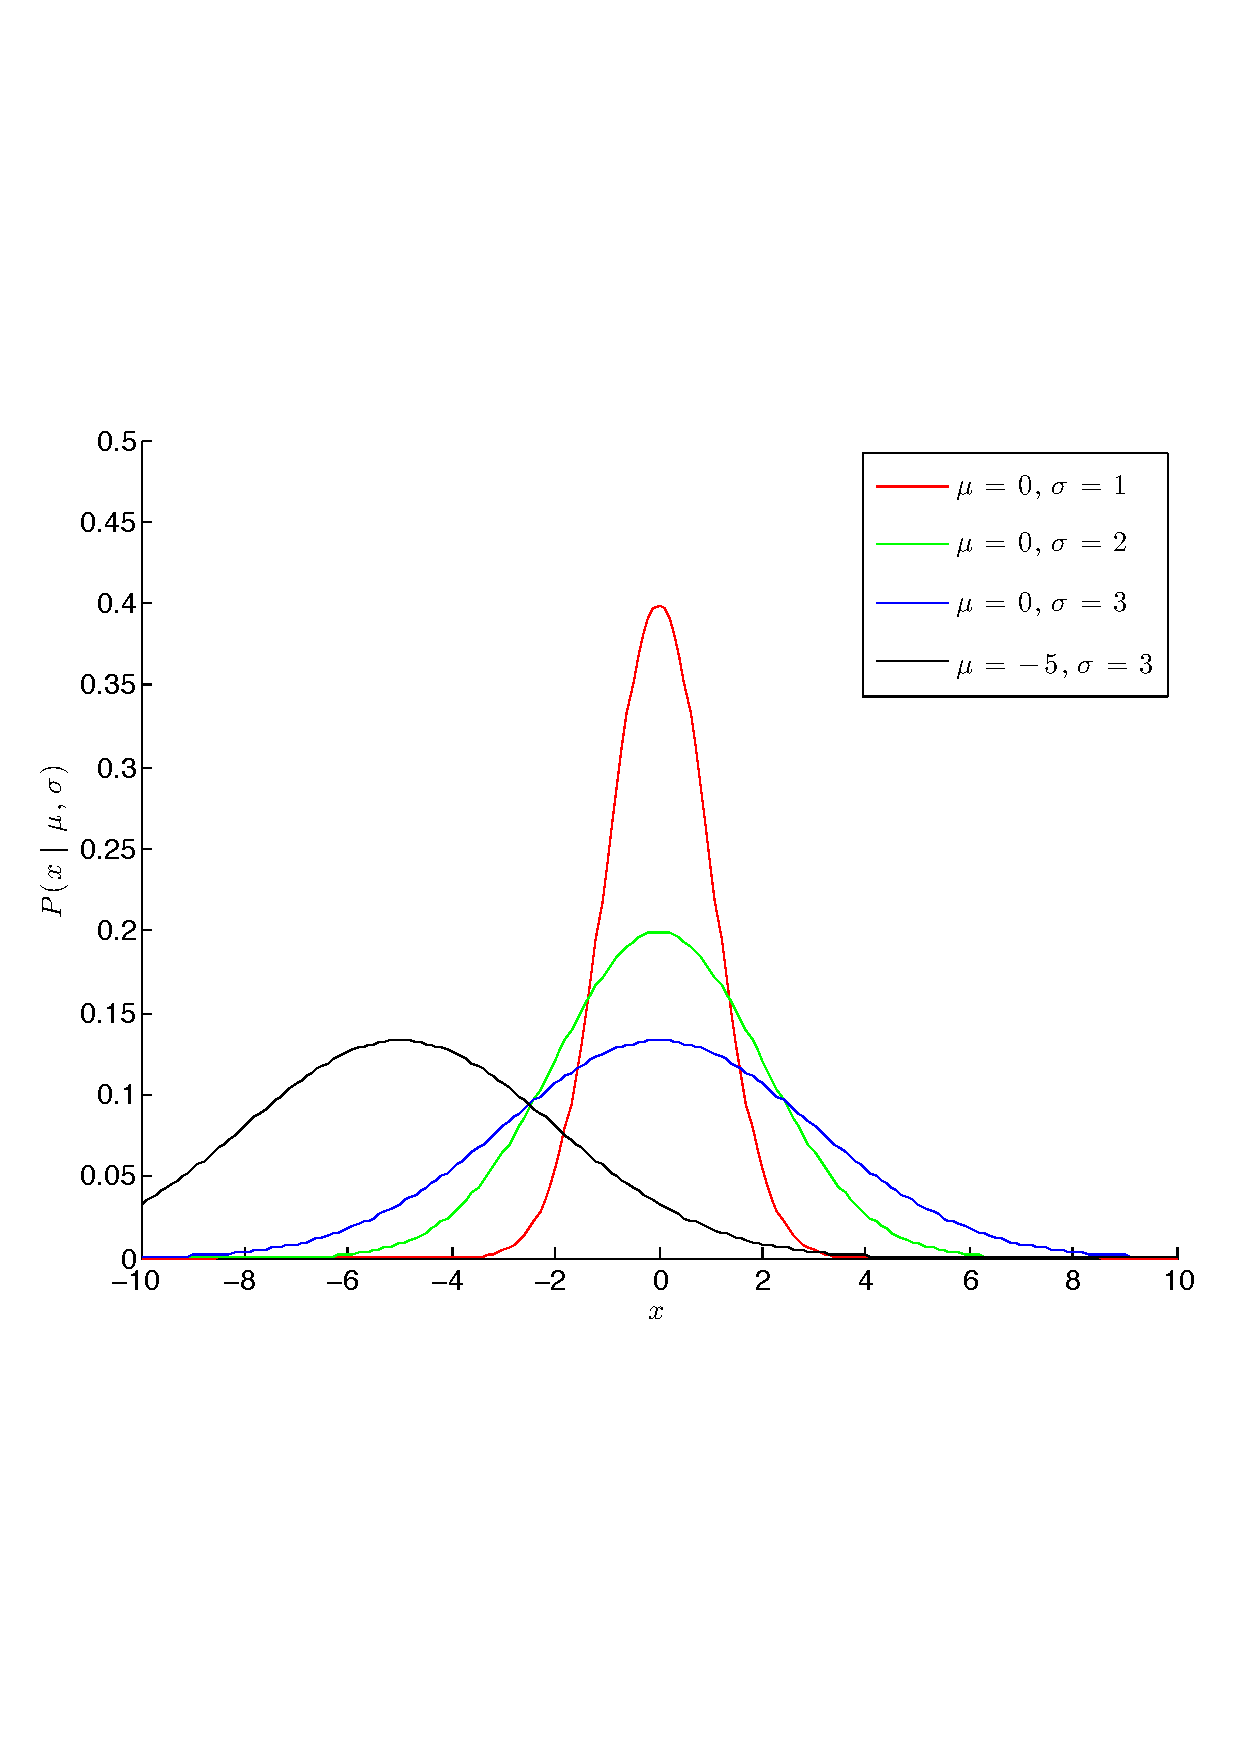
\includegraphics[width=0.38\textwidth]{figures/normalPDF.pdf}
	\caption{\emph{Some normal probability density functions.}}
	\label{fig:normPDF}
\end{wrapfigure}
The normal distribution is a continuous probability distribution that is of primary importance mainly due to the central limit theorem\footnote{The central limit theorem states that under some commonly met conditions, the distribution of the sum of a large number of independent random variables tends towards a normal distribution.}. Its probability density function (pdf) is a bell-shaped, symmetric distribution defined by two parameters. The pdf for a normal distribution is
\begin{align}
	P(x \mid \mu, \sigma) = \frac{1}{\sqrt{2 \pi \sigma^2}} 
	e^{-\frac{(x-\mu)^2}{2 \sigma^2}}
	\label{eq:normalpdf}
\end{align}

where the parameter $\mu$ is the average, the parameter $\sigma$ is the standard deviation (and $\sigma^2$ is the variance), and $P(x \mid \mu, \sigma)$ is to be read as the probability of obtaining measurement $x$ under the assumption that the parameters are $\mu$ and $\sigma$.




%----------------------------------------------------------------------------
\subsection{The binomial distribution}
The Binomial distribution is a discrete probability distribution. It gives the probability of obtaining $x$ successes out of a series of $n$ Bernoulli trials\footnote{A Bernoulli trial is an experiment with exactly two possible outcomes: success with constant probability $p$ and failure with constant probability $q = 1-p$. A single coin flip is a typical example of a Bernoulli trial.}, where the probability of success is $p$ and the probability of failure is $q = 1-p$. The probability mass function (pmf) is
\begin{align}
	P(x \mid p, n) &= {{n}\choose{x}} p^x (1-p)^{n-x},\ \ \ \ \ x = 0, 1, ... n
	\nonumber\\
	%
	&= \frac{n!}{x!(n-x)!}p^x (1-p)^{n-x} 
	\label{eq:binomial}
\end{align}

\setlength\intextsep{0pt}
\begin{wrapfigure}{r}{0.38\textwidth}
	\centering 
	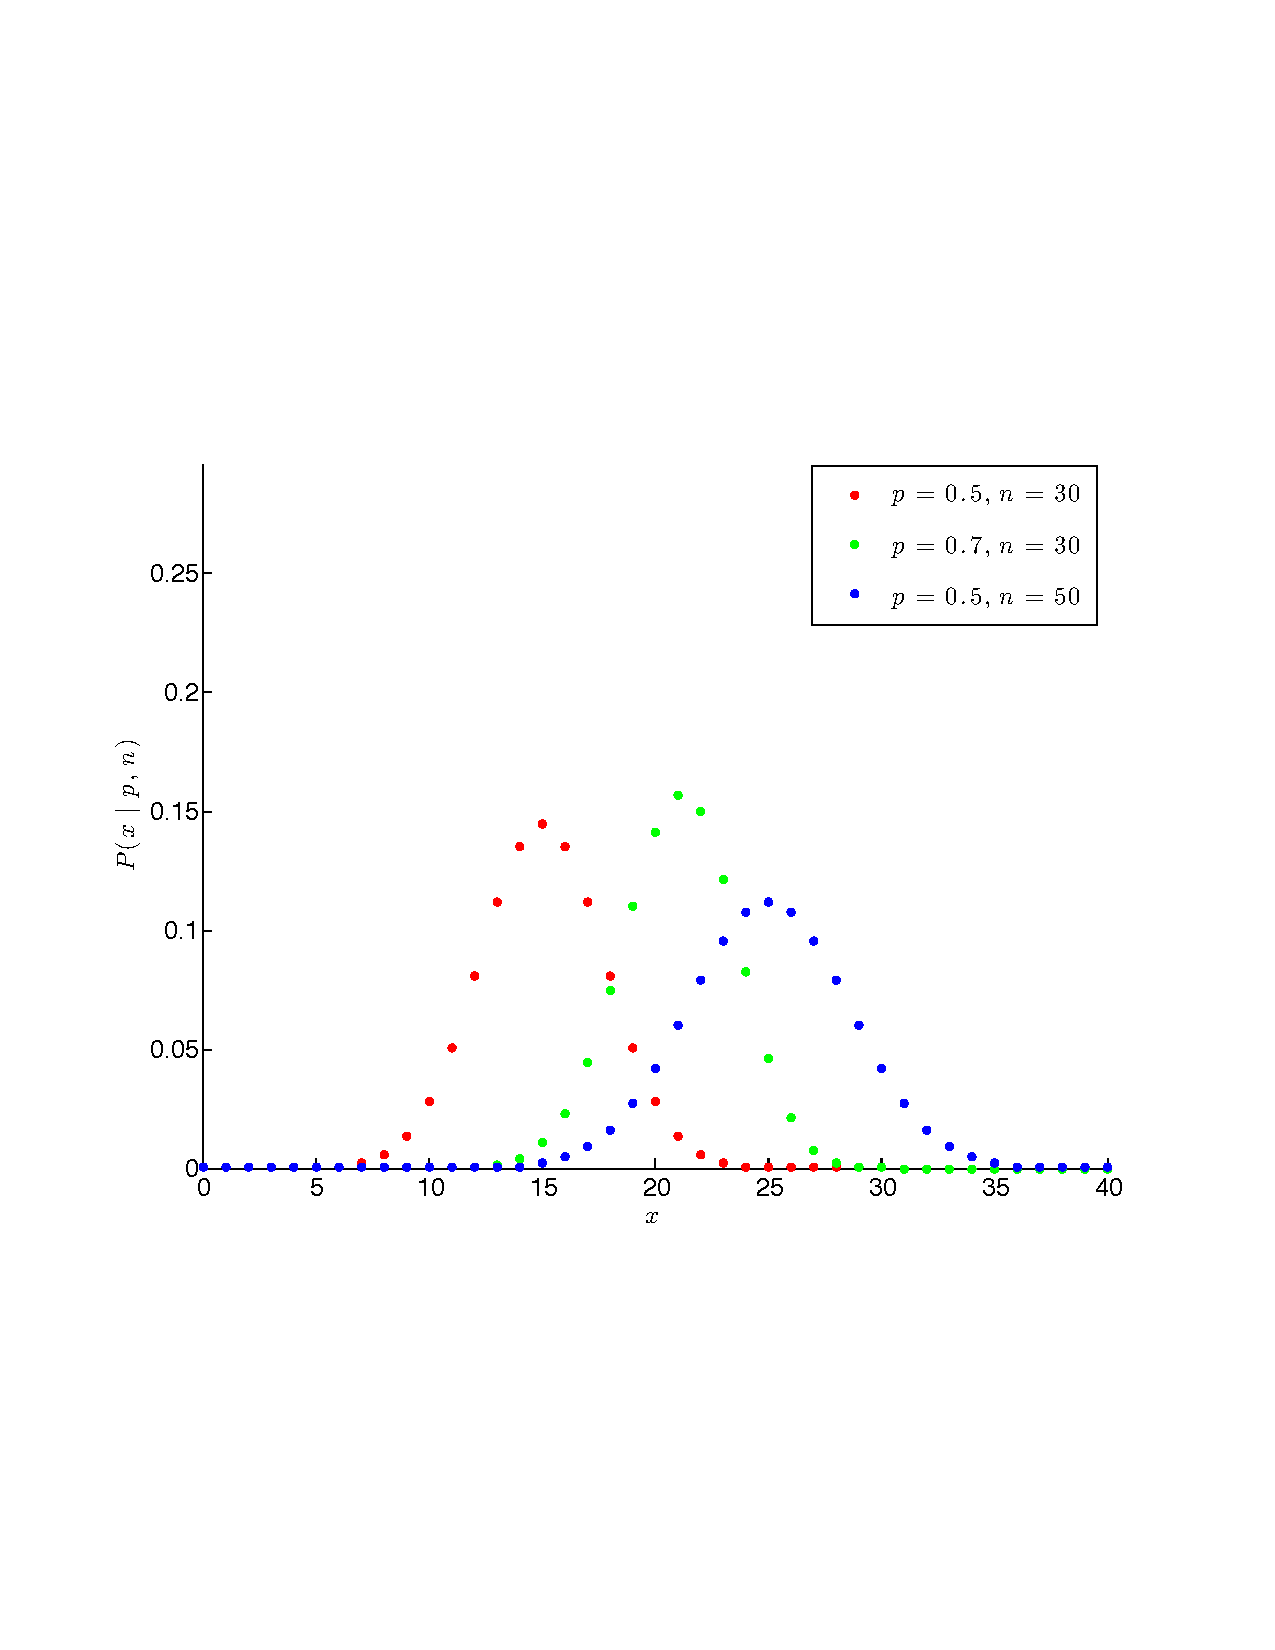
\includegraphics[width=0.38\textwidth]{figures/binomPMF}
	\caption{\emph{Some binomial probability mass functions.}}
	\label{fig:binomPMF}
\end{wrapfigure}
\intextsep\skip32
For a single Bernoulli trial the probability of success is $p$. Because a binomial distribution is a series of $n$ Bernoulli trials with probability of success $p$, the average of a binomial distribution is
\begin{align}
	\mu_{binom} = np
\end{align}

The variance of a binomial distribution can be found by first considering the variance of a Bernoulli distribution
\begin{align}
	\sigma^2_{Bernoulli} &= E[x^2] - (E[x])^2
	\nonumber\\
	%
	&= P(x=1).1^2 + P(x=0).0^2 - (p)^2
	\nonumber\\
	%
	&= p - p^2
	= p(1-p)
\end{align} 

and again because a binomial distribution is a series of $n$ Bernoulli trials, the variance of a binomial distribution is
\begin{align}
	\sigma^2_{binom} = np(1-p)
\end{align}




%----------------------------------------------------------------------------
\subsection{The Poisson distribution}
\setlength\intextsep{0pt}
\begin{wrapfigure}{r}{0.38\textwidth}
	\centering 
	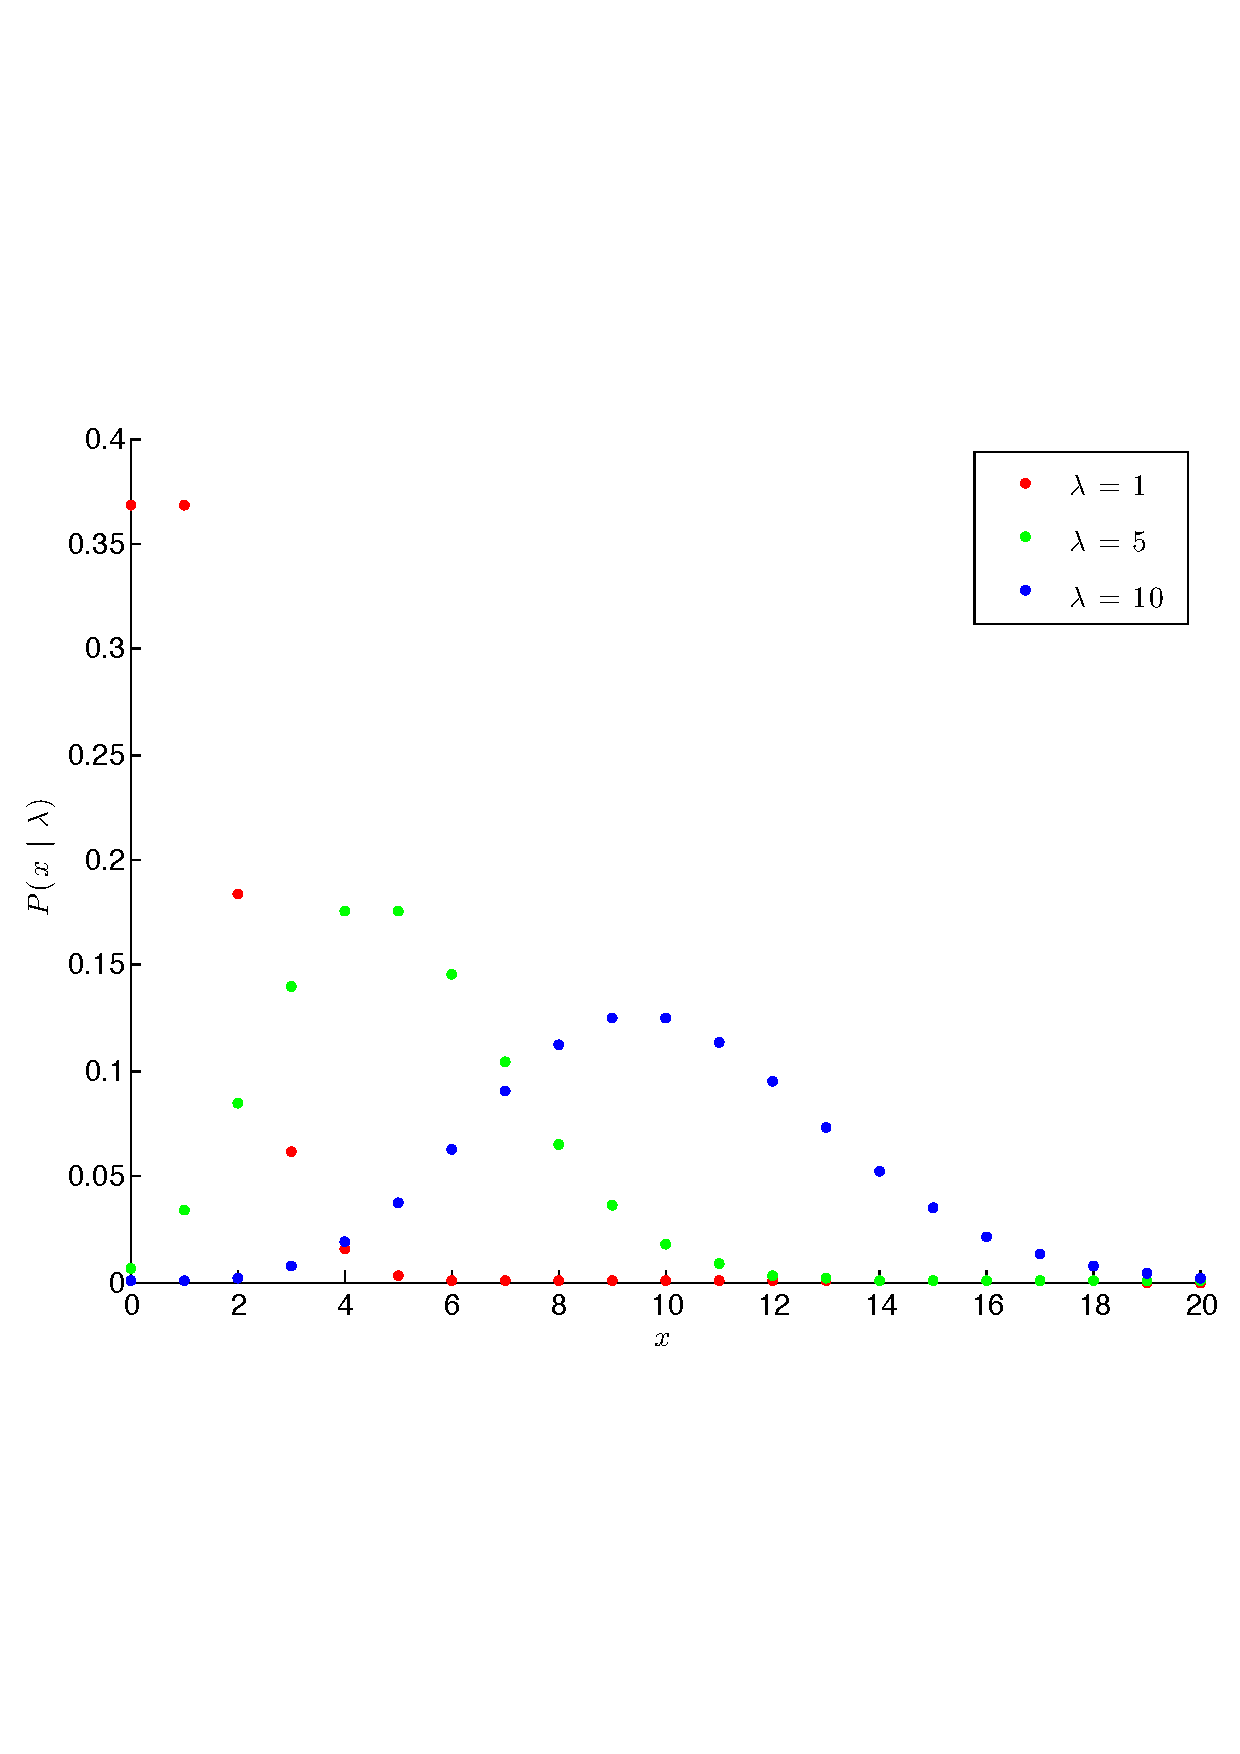
\includegraphics[width=0.38\textwidth]{figures/poissPMF}
	\caption{\emph{Some Poisson probability mass functions.}}
	\label{fig:poissPMF}
\end{wrapfigure}
\intextsep\skip32
The Poisson probability distribution is a discrete probability distribution that gives the probability of observing $x$ events in a certain fixed interval $\tau$ (of time or of space) if the events occur at a known average rate $\lambda$ and if the events are stochastically independent.

An important example of a Poisson process is radioactive decay. This makes the Poisson distribution the prominent one in nuclear medicine.\\

The Poisson distribution can be seen as the limit of a binomial distribution where the number of trials $n$ is very large and the probability of success $p$ is small. With this in mind, the Poisson distribution can be derived from the binomial distribution. 

To derive the distribution, start from eq. \ref{eq:binomial}, and consider the distribution as being a function of the expected number of successes. The expected number of successes is $np$, which will be noted as the parameter $\lambda \equiv np$. With this notation eq. \ref{eq:binomial} becomes
\begin{align}
	P(x \mid n,\lambda) 
	&= \frac{n!}{x!(n-x)!} \left(\frac{\lambda}{n}\right)^x 
	\left(1-\frac{\lambda}{n}\right)^{n-x}
\end{align}
	
Taking the limit for a very large amount of events
\begin{align}
	P_{Poiss}(x \mid \lambda) &\equiv \lim_{n \to \infty} P_{binom} (x \mid n,\lambda )
	\nonumber\\
	%
	&= \lim_{n \to \infty} \frac{n(n-1)...(n-x+1)}{x!}\frac{\lambda^x}{n^x}
	\left ( 1-\frac{\lambda}{n}\right)^{n-x}	
\end{align}

Notice that in this expression, there are $x$ factors in the numerator. Distribute the denominator $n^x$ evenly over all the $x$ factors to get
\begin{align}
	&= \lim_{n \to \infty} \frac{n}{n}.\frac{n-1}{n}.\ ...\ .\frac{n-x+1}{n}
	.\frac{\lambda^x}{x!}
	\left ( 1-\frac{\lambda}{n}\right)^{n-x}
	\nonumber\\
	%
	&= \lim_{n \to \infty} 1.\frac{n-1}{n}.\ ...\ .\frac{n-x+1}{n}
	.\frac{\lambda^x}{x!}
	\left ( 1-\frac{\lambda}{n}\right)^{n}
	\left ( 1-\frac{\lambda}{n}\right)^{-x}	
\end{align}

If $x$ and $\lambda$ are kept constant and the limit is considered, the first $x$ fractions will go to $1$. The factor $\frac{\lambda^x}{x!}$ does not depend on $n$ and remains unchanged. The factor $( 1-\frac{\lambda}{n})^{n}$ is known to go to $e^{-\lambda}$, and the last factor tends to 1 as well. So finally
\begin{align}
	P_{Poiss}(x \mid \lambda) &\equiv \lim_{n \to \infty} P_{binom} (x \mid n,\lambda )
	= \frac{\lambda^x e^{-\lambda}}{x!}
\end{align}
\hfill\\

Because the Poisson distribution plays such a central role in nuclear medicine, it is worth determining its expected value and its variance. The expected value is trivial
\begin{align}
	E[x] = \lambda
\end{align}

Finding the variance is a bit harder. Start from the general expression for the variance
\begin{align}
	\sigma^2 = E(x^2) - [E(x)]^2
\end{align}

from the previous proof, $E(x) = \lambda$ and
\begin{align}
	E(x^2) &= \sum_{x = 0}^{\infty} x^2 P(x)
	= \sum_{x = 0}^{\infty} x^2 \frac{\lambda^x}{x!}e^{-\lambda}
	\nonumber\\
	%
	&= e^{-\lambda} \lambda \left[ 
	\sum_{x = 1}^{\infty} \frac{x}{(x-1)!}\lambda^{x-1} \right]
	\nonumber\\\
	%
	&= e^{-\lambda} \lambda \left[ 
	\sum_{x = 1}^{\infty} \frac{(x-1)}{(x-1)!}\lambda^{x-1} + 
	\sum_{x = 1}^{\infty} \frac{1}{(x-1)!}\lambda^{x-1}\right]
	\nonumber\\\
	%
	&= e^{-\lambda} \lambda \left[ 
	\sum_{x = 2}^{\infty} \frac{1}{(x-2)!}\lambda^{x-2} \lambda + 
	\sum_{x = 1}^{\infty} \frac{1}{(x-1)!}\lambda^{x-1}\right]
	\nonumber\\\
	%
	&= e^{-\lambda} \lambda \left[\lambda e^\lambda + e^\lambda \right]
	= \lambda^2 + \lambda
\end{align}


So the variance of the Poisson distribution is
\begin{align}
	\sigma^2 &= [E(x^2)] - [E(x)]^2
	= [\lambda^2 + \lambda] - [\lambda]^2
	= \lambda
\end{align}




%----------------------------------------------------------------------------
%Statistical parameter estimation
%----------------------------------------------------------------------------
\subsection{Statistical parameter estimation}
The aim of statistical parameter estimation is as the name suggests to try to estimate the values of parameters from some data which has some randomness in it. The parameters are determinant of some physical setting such that their values influence the measured data. Remark that a parameter estimation is not an approximation, but rather a probabilistic interpretation of the parameters.\\

The concept of an estimator is central in parameter estimation problems. An estimator tries to estimate the value of a parameter and can be any function of the data that does not depend on the true, unknown values of the parameters. If an estimator can be any function of the data, then the possibilities for an estimator are endless and clearly some will be better than others. In general a good estimator is one that has no bias, is consistent and efficient... but an estimator with these properties is not always guaranteed to exist! The different concepts presented here will be discussed in detail later.




%----------------------------------------------------------------------------
\subsubsection*{Notation}
Before introducing the key concepts of parameter estimation, the notation and general mathematical framework in which parameter estimation takes place needs to be properly and unambiguously defined.\\

The first concepts to be defined are the population and a sample. The population is noted as $\Omega$. It is the set of all possible outcomes of an experiment. The population can possibly be infinite and/or impossible to observe. 

A trivial example is a coin flip. The population is $\Omega = \{\text{(heads), (tails)}\}$. 

A good example of an infinite population is the generation of a random natural number. Here the population is $\Omega = \mathbb{N}$. 

As a last example for an unobservable population: the height of all men ever. This is a very large (though not infinite) population that can not be observed because many men are not yet born.

Because some populations can not be observed as a whole for a variety of reasons, an experimentalist will often only take a sample of a population. A sample is simply an observable subset of a population that can be used to infer information about the population as a whole. Obviously the sample has to be chosen in such a way that it is representative for the population. Larger samples generally lead to better estimations.\\

Suppose that a certain experiment produces data with some randomness and a certain distribution. Often (and in all applications in this thesis) the data's distribution is known. The aim is then to estimate the distribution's parameters.\\

The data is measured by one or multiple detectors. If there are multiple detectors, the data is noted as $\vec y$ where each component $y_i$ is the data measured by detector $i$ and the index $i \in [1,m]$ corresponds to the $m$ detectors of the experiment. 

If a certain measurement is repeated a number of times $l$, the repeated measurements of the same quantity are noted as $Y = \{{\vec y}_{(1)}, {\vec y}_{(2)}, ..., \vec y_{(k)}, ... \vec y_{(l)}\}$ where the index $k \in [1,l]$ is placed in brackets to stress the difference between $y_i$ which is one measurement by detector $i$ and ${\vec y}_{(k)}$ which is the $k$'th repetition of the measurements performed by the $m$ detectors.\\

The distribution(s) being studied are determined by one or multiple parameters. If there are multiple parameters they are noted as $\vec x$ where each component $x_j$ is the $j$'th parameter of the distribution and the index $j \in [1,n]$ corresponds to the $n$ parameters of the distribution(s).\\

For example if the distribution of the data is assumed to be Poisson, the parameter to be estimated is $\vec x = x = \lambda$ because a Poisson distribution is defined by only one parameter $\lambda$. On the other hand if the data is assumed to have a normal distribution, then the two parameters to be estimated are $\vec x = (x_1 = \mu, x_2 = \sigma)$.\\

For a parameter estimation problem the true values of the parameters are obviously unknown. These true values are noted as $\vec x$. There are different methods to perform probabilistic estimations of the parameters. These methods produce estimators which are noted as $\hat{\vec{x}}$. In component notation this reads that $\hat x_j$ is an estimator of the true, unknown parameter $x_j$.

Taking again the example of data with a normal distribution. Then a standard estimator $\hat{\vec x}$ is: $\hat{\vec{x}} =  (\bar x, s) \xrightarrow[\text{estimates}]{} (\mu, \sigma)$\footnote{Here $\bar x$ and $s$ denote the sample mean and sample standard deviation. They are estimators of the population mean $\mu$ and the population standard deviation $\sigma$, which are the true, unknown parameters.}\\

The true distribution of the data is noted as $P(\vec y \mid \vec x)$ where the parameter(s) $\vec x$ are all the parameters that influence the distribution. The distribution that is estimated is noted as $P(\vec y \mid \hat{\vec x})$.




%----------------------------------------------------------------------------
\subsubsection*{Bias}
The bias $b(\hat x)$ is a property of an estimator $\hat x$. It is a measure of the quality of an estimator as it measures how close the expected value of the estimator gets to the true value of the parameter. If the distribution of the estimator $\hat x$ is known or can be reasonably assumed, it is possible to determine its expected value. If $E[\hat x] = x$ the estimator is referred to as unbiased. Bias is defined as:
\begin{align}
	b(\hat x) &= E[\hat x] - x
	\nonumber\\
	%
	&= E[\hat x - x]
	\label{eq:bias}
\end{align}

If two different estimators would have the same properties (variance, computational cost, ...) but one of the estimators would be biased and the other not, the unbiased estimator would be preferred. In real situations two different estimators do not have the same properties and a biased estimator may be preferred if its other properties make it more useful. For example if an unbiased estimator does not exist without further assumptions or if its variance is unacceptably large or if it is computationally very expensive, a biased estimator may be preferred. Often the bias of an estimator that is being used is small. The textbook examples of unbiased estimators are the sample mean
\begin{align}
	\bar x = \frac{1}{l}\sum_{k=1}^l y_{(k)}
	\label{eq:samplemean}
\end{align}

and the sample variance
\begin{align}
	s^2 = \frac{1}{l-1}\sum_{k=1}^l \left( y_{(k)} - \bar x \right)^2
\end{align}

It is worth noting that the proofs \cite{Watkins} of the unbiasedness of $\bar x$ and $s^2$ only assume that the measurements are independent. Therefore these results are always valid for independent measurements, regardless of their distribution.




%----------------------------------------------------------------------------
\subsubsection*{Consistency}
Suppose there are $l$ repeated (scalar) measurement of some quantity: $Y = \{y_{(1)}, ..., y_{(l)}\}$ and suppose an estimator $\hat x$ is determined from this sample. The estimator is consistent if it converges to the parameter's true value when the amount of data increases. Any estimator for which
\begin{align}
	\lim_{l\to\infty} P\left( \mid \hat x - x \mid \geq \varepsilon \right) = 0,\ \ \ \ \
	\forall \epsilon \geq 0 
\end{align}

holds is referred to as a consistent estimator. Alternatively an estimator is consistent if and only if it is asymptotically unbiased $(\lim_{l\to\infty} E[\hat x] = x)$ and if its variance goes to zero $(\lim_{l\to\infty} var(\hat x) = 0)$.\\
A good example of a consistent estimator is (again) the sample mean.

\theorem
{
The sample mean $\bar x$ of a normal distribution is a consistent estimator of the population mean $\mu$.
}
{
Given a sample $Y = \{y_{(1)}, ..., y_{(l)}\}$ of $l$ measurements sampled from a normal distribution $P(\mu, \sigma)$. The sample mean is given by eq. \ref{eq:samplemean} and is an unbiased estimator of the population mean $\mu$.

Because the sample mean is unbiased, the first condition is met
\begin{align}
	E[\hat x] = x \Rightarrow \lim_{l\to\infty} E[\hat x] = x
\end{align}

and because the distribution is normal, the estimator $\bar x$ is also normally distributed with mean $\mu$ and variance $\sigma^2/l$. Therefore
\begin{align}
	\lim_{n\to\infty} var(\bar x) = \lim_{l\to\infty} \frac{\sigma^2}{l} = 0
\end{align}

So both conditions are met and the sample mean is a consistent estimator of the population mean.
}




%----------------------------------------------------------------------------
\subsubsection*{Efficiency}
The efficiency of an estimator is a measure of how wide the distribution of the estimator is. The more efficient an estimator is, the narrower its distribution. It will be proven that there exists a lower bound for the variance of any estimator referred to as the Cramer-Rao bound (eq. \ref{eq:raocramer}). The efficiency measures how close the estimator's variance gets to this best possible variance. The efficiency of a single unbiased estimator is defined as
\begin{align}
	\epsilon(\hat x) = \frac{1/I(x)}{var(\hat x)}
	\label{eq:efficiency}
\end{align}

where $I(x)$ is the Fisher information (which will be discussed later).  If $e(\hat x) = 1$ for all $x$, the estimator is referred to as an efficient estimator.\\

Before deriving the Cramer-Rao bound some new concepts must be introduced first:\\
- Likelihood\\
- Information\\
- Score\\
These concepts will allow to determine the lower bound on the variance of any estimator.




%----------------------------------------------------------------------------
\subsubsection*{Likelihood}
The likelihood $\mathcal{L}(\vec x \mid \vec y)$ is a function of the parameter $\vec x$ of a statistical model, given some data $\vec y$. It takes as input the possible values of the parameter and returns the probability that the data is what it is observed to be. So the likelihood is the probability that the data is what it is, assuming the parameter is a certain $\vec x$. It is \emph{not} the probability that the parameter is a certain $\vec x$!\\

If the measurements in $\vec{y}$ are assumed to be stochastically independent, then the likelihood is the product of the probability of every single measurement $y_i$, for arbitrary parameter $\vec x$. It is expressed as
\begin{align}
	\mathcal{L}(\vec x \mid \vec y) = 
	\prod_{i=1}^{m} P\left( y_i \mid \vec x \right)
	\label{eq:likelihood}
\end{align}

This returns the probability of obtaining the measured data, assuming a certain value for the parameter.\\

The likelihood is often used to find the parameter value(s) that maximise the likelihood of the data (Maximum Likelihood (ML) methods). In such methods, the value of importance is the maximum of the likelihood. Because the likelihood is a product, and because the logarithm of a product is the sum of the logarithms, and because the likelihood and its logarithm have their maximum at the same value, the log-likelihood is often used in ML methods. The log-likelihood is
\begin{align}
	\ell = ln\ \mathcal{L} \left( \vec x \mid \vec y \right)
	= \sum_{i=1}^{m} ln\ P(y_i\mid\vec x)
	\label{eq:logLikelihood}
\end{align}

\begin{figure}[h]
	\begin{minipage}[b]{.499\linewidth}
 		\centering
 		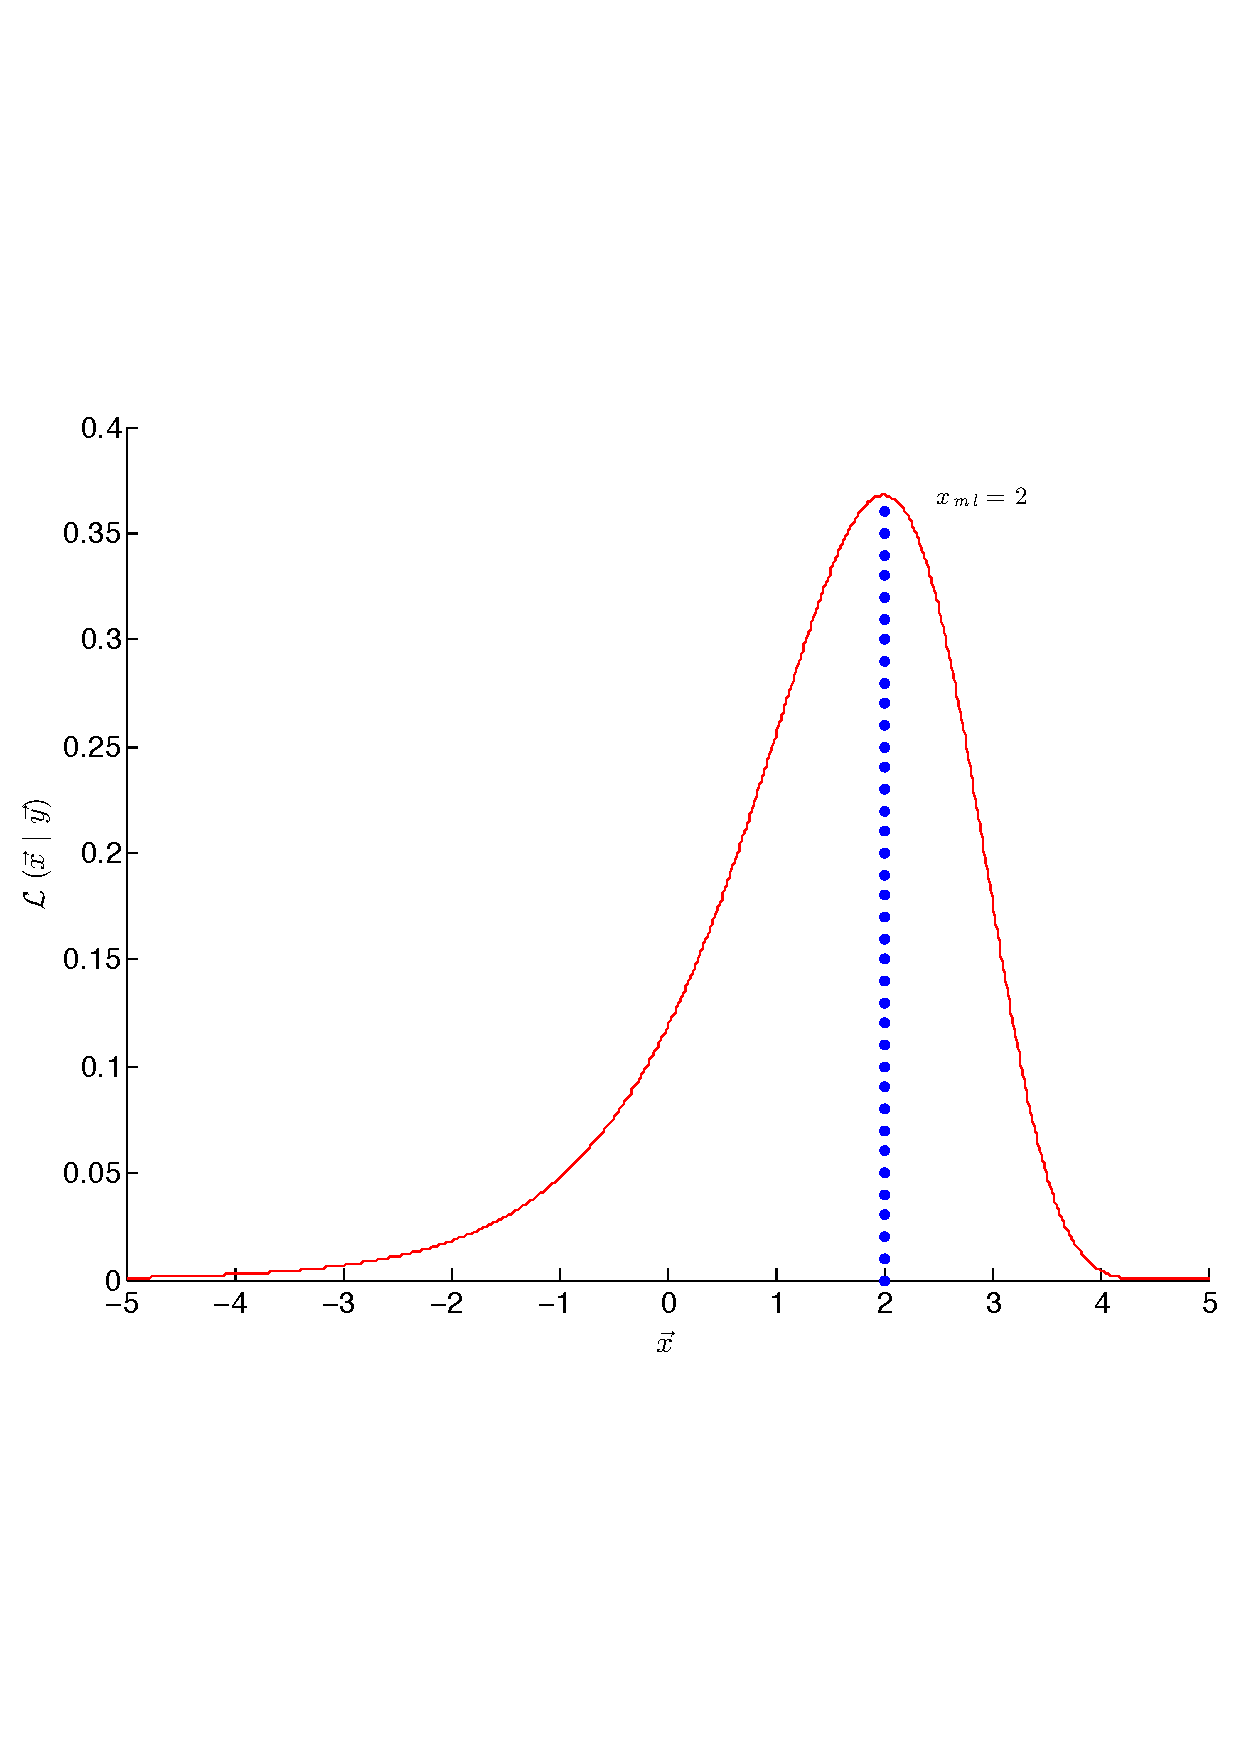
\includegraphics[width=\linewidth]{figures/likelihood}
	\end{minipage}
	\begin{minipage}[b]{.499\linewidth}
 	  	\centering
 	  	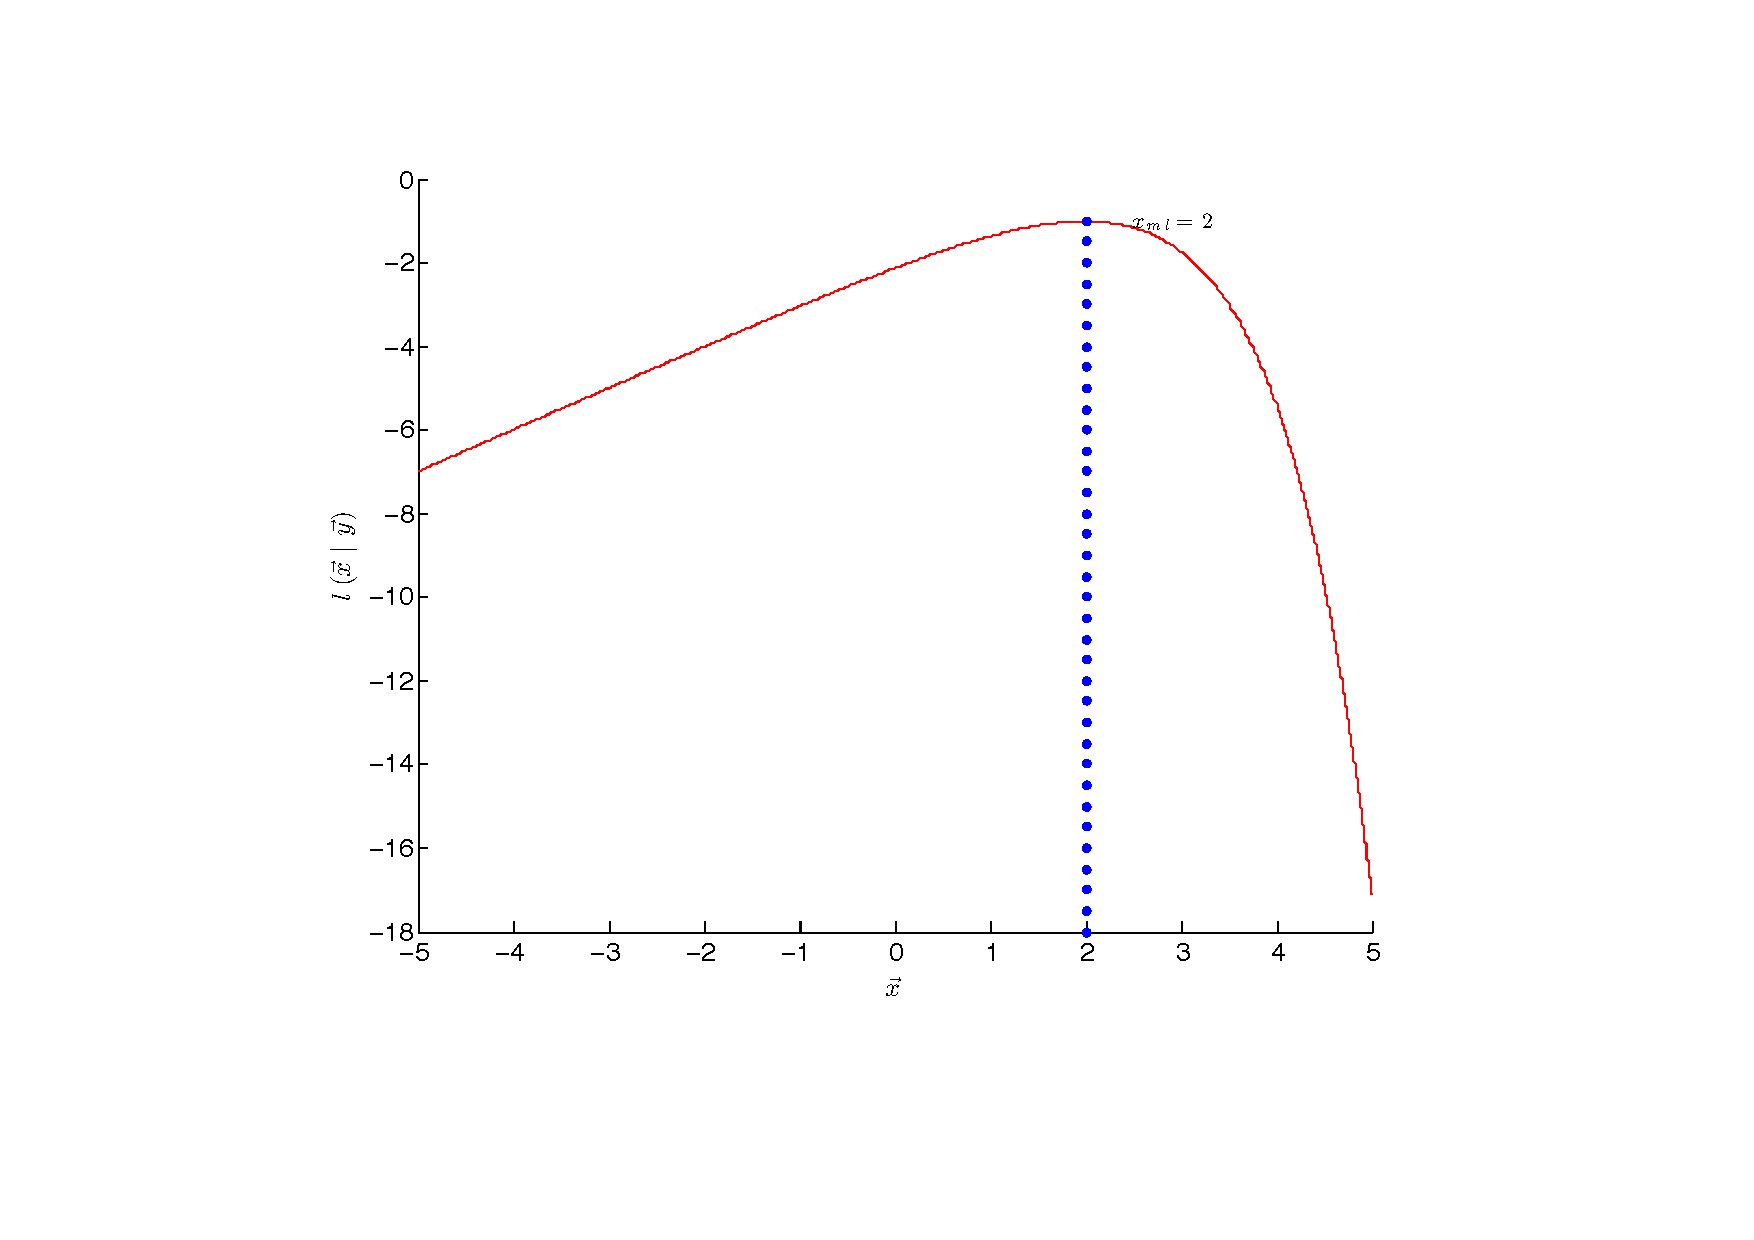
\includegraphics[width=\linewidth]{figures/log-likelihood}
	\end{minipage}
	\caption{\emph{An example of a likelihood function on the left and its corresponding log-likelihood on the right. Remark that both functions have their maximum at the same parameter value $x = x_{ML} = 2$.}}
	\label{fig:likelihood}
\end{figure}




%----------------------------------------------------------------------------
\subsubsection*{Information}
In the current context, information refers to the "Fisher"-information. The concept of information captures three ideas:
\begin{enumerate}
	\item If the amount of data doubles, the amount of information must double as well.
	
	\item If some (sub)set of data is not influenced by some parameter $x$, then the information about that parameter contained in the set must be $0$.

	\item Information must be related to precision. If more information is available, the estimation of the parameter must be more precise, which implies that the variance decreases.
\end{enumerate}

The Fisher information $I_{\vec y}(x)$ (read as the information contained in the data $\vec y$ about the parameter $x$) about a single, scalar parameter $x$ given data $\vec y$ is defined as
\begin{align}
	I_{\vec y}(x) &= E\left[ \left( \frac{\partial\ ln\ 
	\mathcal{L} \left( x \mid \vec y \right)}
	{\partial x} \right)^2 \right]
	= E\left[ \left( \frac{\partial \ell}{\partial x} \right)^2 \right]
	\nonumber\\
	%
	&= \int_{\Omega_{x}} \left( \frac{\partial\ ln\ 
	\mathcal{L}(x \mid \vec y)}
	{\partial x} \right)^2 \mathcal{L} \left( x \mid \vec y \right) d\vec y
	\label{eq:b}
\end{align}

where the likelihood is assumed to be differentiable\footnote{For nuclear imaging the likelihood is a product of Poisson probabilities $P(y) = \frac{x^y e^{-x}}{y!}$, which is differentiable with respect to the parameter $x$.}. If there is not $1$, but $n$ different parameters to be estimated from the data, the information becomes a $[n \times n]$ matrix
\begin{align}
	\left[ I_{\vec y} (\vec x) \right]_{jj'} &= 
	E\left[\frac{\partial\ ln\ \mathcal{L} \left( \vec x \mid \vec y \right)}
	{\partial x_j}.
	\frac{\partial\ ln\ \mathcal{L} \left( \vec x \mid \vec y \right)}
	{\partial x_{j'}} \right]
	\nonumber\\
	%
	&= \int_{\Omega_{\vec x}} 
	\frac{\partial\ ln\ \mathcal{L} \left( \vec x \mid \vec y \right)}
	{\partial x_j}.
	\frac{\partial\ ln\ \mathcal{L} \left( \vec x \mid \vec y \right)}
	{\partial x_{j'}} \mathcal{L} \left( \vec x \mid \vec y \right) d\vec y
	\label{eq:fisherInformation}
\end{align}

This notation is quite cumbersome. It can be simplified by introducing the score. The score measures how sensitive a likelihood function is to a parameter. For a single measurement of some quantity the score is defined as
\begin{align}
	S(x \mid y) = \frac{\partial}{\partial x}\left( ln\ P(y \mid x) \right)
\end{align}

If the data consists not of $1$ but of $m$ measurements, the score is
\begin{align}
	S(x \mid \vec y) &= \sum_{i=1}^{m} S(x \mid y_i )
	= \sum_{i=1}^{m} \frac{\partial}{\partial x} (ln\ P(y_i \mid x))
	\nonumber\\
	%
	&= \frac{\partial}{\partial x} \sum_{i=1}^{m} ln\ P(y_i \mid x)
	= \frac{\partial ln\ \mathcal{L}(x \mid \vec y)}{\partial x}
\end{align}

Remark that the score itself is a random variable. If the experiment were to be repeated, a different data set $\vec y$ would be observed and this data set would have a different score. 

\theorem
{
Suppose that the sample space $\Omega_{\vec x}$ is independent of the values of the parameter $\vec x$ and that the likelihood is regular enough such that differentiation and integration can be interchanged. Under these conditions, the expected value of the score is 0.
}
{
The proof is a straightforward computation of the expected value of the score. The expected value of the score of a single measurement is
\begin{align}
	E\left[ S(x \mid y) \right] &= E\left[ \frac{\partial}
	{\partial x} ln\ P(y \mid x) \right]
	\\
	%
	\shortintertext{For a single measurement the likelihood is by definition equal to the probability function $P(y \mid x) = \mathcal{L}(x \mid y)$}
	%
	&= \int_{\Omega_x} \frac{\partial ln\ P(y \mid x)}
	{\partial x} P(y \mid x) dy
	\\
	%
	\shortintertext{Taking the derivative of the logarithm}
	&= \int_{\Omega_x} \frac{1}{P(y \mid x)} \left( \frac{\partial}
	{\partial x} P(y \mid x) \right) P(y \mid x) dy
	\\
	%
	&= \int_{\Omega_x} \frac{\partial}{\partial x} P(y \mid x) dy
	\\
	%
	\shortintertext{Because integration and derivation can be interchanged}
	&= \frac{\partial}{\partial x} \int_{\Omega_x} P(y \mid x) dy
	\\
	%
	\shortintertext{The integral of a probability function needs by definition to be 1}
	&= \frac{\partial}{\partial x} . 1 = 0
\end{align}

So the expected value of the score of a single measurement is 0. Because the expected value of the score of a data set is the sum of the scores of the elements of the data set, the expected value of the score of the whole data set is 0 as well
\begin{align}
	E\left[ S(x \mid \vec y) \right] &= 
	\sum_{i=1}^{n}E\left[ S(x \mid y_i ) \right] = 0 + ... + 0 = 0
\end{align}
}\hfill

With the definition of the score and knowing that the expected value of the score is 0, the Fisher information matrix (eq. \ref{eq:fisherInformation}) can be written as the covariance of the score, which is the second raw moment
\begin{align}
	\left[ I_{\vec y}(\vec x) \right]_{jj'} 
	&= E\left[ S(x_j \mid \vec y).S(x_{j'} \mid \vec y) 
	\right]
	= cov[S(x \mid \vec y )]_{jj'} 
\end{align}




%----------------------------------------------------------------------------
\subsection{The Cramer-Rao inequality}
The Cramer-Rao (CR) inequality has been mentioned before. It gives a lower bound on the variance of any estimator. Any estimator whose variance is equal to the CR bound is referred to as efficient ($\epsilon = 1$, eq. \ref{eq:efficiency}). The derivation of the CR bound if given here for problems with only one parameter.

\theorem
{
Assume that the sample space $\Omega_{x}$ is independent of the value of the parameter $x$, that the Fisher information is always defined, and that integration with respect to $y$ and differentiation with respect to $x$ in the expectation of the estimator $\hat x$ can be exchanged.

Under these assumptions the variance of any estimator has a lower bound, the Cramer-Rao bound, given by
\begin{align}
	var[\hat{x}] \geq \frac
	{\left(1 + \frac{\partial}{\partial x}b(\hat x)\right)^2}
	{I_{\vec y}(x)}
	\label{eq:raocramer}
\end{align}

where the bias $b(\hat x)$ is given by \ref{eq:bias} and can be derived to $x$. This inequality also reflects the idea that information should be related to precision.
}
{
Consider an estimator $\hat x = \hat x(\vec y)$ of a parameter $x$ with possibly a bias $b(\hat x) = (E[\hat x] - x)$ and variance $var[\hat x] < \infty$. Determine $E\left[ \hat x . S(x \mid \vec y)\right]$
\begin{align}
	E\left[ \hat x \ S(x \mid \vec y)\right] &=
	\int ... \int \hat x \ S(x \mid \vec y)\ 
	\mathcal{L}(x \mid \vec y)\ d\vec y
	\nonumber\\
	%
	&= \int ... \int \hat x\ \frac{1}{\mathcal{L}(x \mid \vec y)}
	\left( \frac{\partial}{\partial x} \mathcal{L}(x \mid \vec y)
	\right) \ \mathcal{L}(x \mid \vec y)\ d\vec y
	\nonumber\\
	%
	&= \int ... \int \hat x\
	\left( \frac{\partial}{\partial x} \mathcal{L}(x \mid \vec y)
	\right) \ d\vec y
\end{align}

Because derivation and integration can be exchanged this becomes
\begin{align}
	E\left[ \hat x\ S(x \mid \vec y)\right] &= \frac{\partial}{\partial x} \int ... \int \hat x\ \mathcal{L} 
	(x \mid \vec y ) d\vec y
	\nonumber\\
	%
	&= \frac{\partial}{\partial x} E[\hat x]
	= \frac{\partial}{\partial x}\left(x + b(\hat x)\right)
	= 1 + \frac{\partial}{\partial x}b(\hat x)
\end{align}

Having the previous expression allows determining the covariance between the stochastic $\hat x$ and $S(x \mid \vec y)$
\begin{align}
	cov[\hat x, S(x \mid \vec y)] &=
	E\left[ \hat x\ S(x \mid \vec y)\right] 
	- E\left[ S(x \mid \vec y)\right].E\left[ \hat x \right]
	\nonumber\\
	%
	&= 1 + \frac{\partial}{\partial x}b(\hat x) - 
	0.E\left[ \hat x \right]
	=	1 + \frac{\partial}{\partial x}b(\hat x)
\end{align}

and the correlation coefficient is then
\begin{align}
	\rho^2 &= \frac{
	\left( cov[\hat x, S(x \mid \vec y)] \right)^2}
	{var\left[\hat x\right].var\left[S(x \mid \vec y)\right]}
	\nonumber\\
	%
	&= \frac
	{\left(1 + \frac{\partial}{\partial x}b(\hat x)\right)^2}
	{var[\hat x].I_{\vec y}(x)}
\end{align}

Where the fact that the variance of the score is the Fisher information was used.

Finally using that the correlation coefficient $\rho^2 \leq 1$, the CR inequality can be retrieved
\begin{align}
	var[\hat x] \geq \frac
	{\left(1 + \frac{\partial}{\partial x}b(\hat x)\right)^2}
	{I_{\vec y}(x)}
\end{align}
}\hfill

For unbiased estimators or for estimators whose bias does not depend on the true parameter $x$, the CR bound takes the following elegant form:
\begin{align}
	var[\hat x] \geq I_{\vec y}^{-1}(x)
\end{align}

The previous results are valid for problems where only one parameter is estimated. If there are multiple parameters, the CR bounds are expressed as a matrix product\cite{cramerRaoMultiDim}.
\begin{align}
	cov(\hat{\vec{x}}) \geq \left( \frac{\partial E[\hat{\vec{x}}]}{\partial \vec x} \right) 
	. [I_{\vec y}(\vec x)]^{-1}
	. \left( \frac{\partial E[\hat{\vec{x}}]}{\partial \vec x} \right)^T
	\label{eq:CramerRaoMultiDim}
\end{align}

where $\partial E[\hat{\vec{x}}] / \partial \vec x$ is the Jacobian matrix with elements $J_{jj'} = \partial E[\hat x_j] / \partial x_{j'}$




%----------------------------------------------------------------------------
\subsection{Estimating parameters using maximum likelihood}\label{sec:mlmethod}
One of the more popular methods to estimate statistical parameters is the maximum likelihood method. In all practical parameter estimation problems, some experiment will generate some data $\vec y$. The problem then is to, given that particular data set, find the values $\hat{ \vec x}_{ml}$ of the parameters that are the most likely to have generate the observed data. These values are the ML estimator for the parameter $\vec x$. Note that the ML method produces the parameter estimators that are the most likely to have generated the observed data and not the "most likely" values of the parameters, a common confusion.\\

The ML method is based on the likelihood function. If the data $\vec y$ is fixed and assuming that the distribution of the data is known, or can be reasonably approximated, it is possible to determine the likelihood function $\mathcal{L}(\vec x \mid \vec y)$. It is a function of the data $\vec y$ and the parameter $\vec x$. Since the data  is fixed, the likelihood only depends on the value of the parameter. A ML estimator is then defined as
\begin{align}
	\hat{ \vec x}_{ml} = arg_{\vec{x}}max\ 
	\mathcal{L} \left( \vec x \mid \vec y \right)
\end{align}
	
So $\hat{ \vec x}_{ml}$ can indeed be interpreted as being the values of the estimators $\hat{ \vec x}$ that maximise\footnote{Beware of the distinction between local and global extrema.} the probability of obtaining the measured data set.\\

The likelihood is (eq. \ref{eq:likelihood})
\begin{align}
		\mathcal{L}(\vec x \mid \vec y) = 
	\prod_{i=1}^{m} P\left( y_i \mid \vec x \right)
\end{align}

and the log-likelihood (eq. \ref{eq:logLikelihood})
\begin{align}
		\ell = ln\ \mathcal{L} \left( \vec x \mid \vec y \right)
	= \sum_{i=1}^{m} ln\ P(y_i\mid\vec x)
\end{align}

The maximum likelihood parameter estimation method then consists of determining the values of the parameter $\vec x$ that maximises the likelihood. The ML estimators are therefore found by solving
\begin{align}
	\hat{ \vec x}_{ml} = \{{x_j}\}\ : \ \left(
	S(x_j \mid \vec y ) = 
	\frac{\partial ln\ \mathcal{L} (\vec x \mid \vec y)}
	{\partial\ x_j} = 0 \right),\ \ \ \ \ 
	\forall j \in [1,n] 
	\label{eq:ml}
\end{align}




\subsubsection*{Example}
Suppose some data $\vec y = \{y_i\}$ is given of some continuous quantity where each individual measurement can have a different though known precision $\{\sigma_i\}$. Suppose the data has a normal distribution with average $\mu$. Here $\mu$ is the parameter to be estimated. The probability density function for the data is normal
\begin{align}
	P(y_i \mid \vec x) = P(y_i \mid \mu, \sigma_i) = \frac{1}{\sigma_i \sqrt{2 \pi}} 
	e^{-\frac{(y_i-\mu)^2}{2 \sigma_i^2}}
\end{align}

from the probability density function, it is straight forward to get the log-likelihood
\begin{align}
	\ell = ln\ \mathcal{L} \left(\mu, \sigma_i \mid \vec y \right)
	&= \sum_{i=1}^{n} ln\ P(y_i \mid \mu, \sigma_i)
	\nonumber\\
	%
	&= \sum_{i=1}^{n} -ln\left( \sigma_i\sqrt{2\pi}\right) - 
	\sum_{i=1}^{n} \frac{(y_i-\mu)^2}{2 \sigma_i^2}
	\label{eq:mlExample}
\end{align}


To estimate the parameter $\mu$, eq. \ref{eq:mlExample} needs to be derived to $\mu$ as prescribed in eq. \ref{eq:ml}. If the order of differentiation and summation can be inverted
\begin{align}
	S\left(\mu, \sigma_i \mid \vec y \right) &=
	\frac{\partial ln\ \mathcal{L} \left(\mu, \sigma_i \mid \vec y \right)}
	{\partial\ \mu}
	= \sum_{i=1}^{n} \frac{y_i-\hat\mu}{\sigma_i^2} = 0
	\nonumber\\
	%
	\Rightarrow \hat\mu_{ml} &= \frac
	{\sum_{i=1}^{n} y_i / \sigma_i^2}
	{\sum_{i=1}^{n} 1/\sigma_i^2}
\end{align}

which concludes this example on how to find an ML estimator.\\

The ML estimator (when it exists) has some nice properties which make it a likeable estimator. Its two most important properties will be given. Only one proof will be given and only for a scalar parameter $x$.

\theorem
{
If there exists an estimator that is unbiased and efficient, then this estimator is the ML estimator $\hat x_{ml}$. 
}
{
Suppose that for a certain problem there is an estimator $\hat x'$ for the parameter $x$ that is a function of the data $\vec y$, and suppose that $\hat x'$ is both unbiased and efficient.\\

The estimator $\hat x'$ is efficient if its variance is minimal which implies reaching the CR bound. So the CR inequality becomes an equality. From the derivation of the CR bound it should be clear that this is the case if the correlation coefficient $\rho$ between the score $S(x \mid \vec y)$ and the estimator $\hat x'$ equals $\pm 1$.\\

If $\rho = \pm 1$ then by definition there must exist a linear relation between $S(x \mid \vec y)$ and $\hat x'$. This linear relation can be written as
\begin{align}
	S(x \mid \vec y) = a(x).\hat x' + b(x)
	\label{eq:linearMLRelation}
\end{align}

The relation \ref{eq:linearMLRelation} holds for all values of the parameter $x$, so it also holds for the ML estimator $\hat x_{ml}$. For the ML estimator, the score is by definition $0$ and therefore 
\begin{align}
	S(\hat x_{ml} \mid \vec y) &= 0
	\nonumber\\
	%
	\Rightarrow \hat x' &= -\frac{b(\hat x_{ml})}{a(\hat x_{ml})}
\end{align}

It has already been proven that the expected value of the score is $0$. Therefore
\begin{align}
	E\left[ S(x \mid \vec y) \right] &= 
	a(x)\ E\left[ \hat x' \right] + b(x) = 0
	\nonumber\\
	%
	\Rightarrow E\left[ \hat x' \right] &= -\frac{b(x)}{a(x)}
	\label{eq:a}
\end{align}


This also holds for all values of the parameter $x$ and in particular for $\hat x_{ml}$
\begin{align}
	\Rightarrow E_{x=\hat x_{ml}}\left[\hat x' \right]
	= -\frac{b(\hat x_{ml})}{b(\hat x_{ml})} = \hat x'
	\label{eq:i}
\end{align}

where $E_{x=\hat x_{ml}}\left[\hat x' \right]$ is the expected value of the estimator $\hat x'$ under the assumption that the parameter $x = \hat x_{ml}$.

Because $\hat x'$ is assumed to be unbiased its expected value is
\begin{align}
	&E\left[ \hat x' \right] = 
	\int \hat x'\ P(\vec y \mid x )\ dy = x
	\label{eq:j}
\end{align}

If the parameter is assumed to be equal to the ML estimator: $x = \hat x_{ml}$, then the expected value of the estimator $\hat x'$ satisfies
\begin{align}
	\hat x' \stackrel{\ref{eq:i}}{=} E_{x=\hat x_{ml}}\left[\hat x' \right] 
	\stackrel{\ref{eq:j}}{=} \hat x_{ml}
\end{align}

So the estimator $\hat x'$ is equal to the ML estimator $\hat x_{ml}$.
}

\theorem
{
If the data consists of $l$ repeated measurements of some quantity: \\
$Y = \{\vec y_{(1)}, \vec y_{(2)}, ... \vec y_{(l)}\}$ \\then a ML estimator $\hat x_{ml}$ is asymptotically ($l \rightarrow \infty$) unbiased and efficient.
}
{
Proofs for this theorem can be found in literature, e.g. \cite{stat2}.
}




%----------------------------------------------------------------------------
\subsubsection*{Subtleties of the ML parameter estimation method}
The asymptotic behaviour of the ML estimators make them likeable, especially when a large data set is available. But some precautions are to be taken when using ML estimators. The ML estimators are found by examining the likelihood function and looking for the parameter values where the likelihood's derivatives vanish. This is where some trouble may arise. The subtleties to be aware of:

\begin{enumerate}
	\item It is possible that the ML estimator found is not a (global) maximum of the likelihood function. Since the likelihood's derivative just has to be 0, it is possible that the found ML estimator is a minimum, a local maximum or even a saddle point of the likelihood.
	
		\item If the likelihood is flat, the ML estimator is not uniquely defined.

	\item If an iterative algorithm is used to find the ML estimator and the likelihood is very flat, it can take the algorithm a long time (= large number of iterations) to converge to the ML estimator.
	
	\item The speed of convergence of an iterative algorithm depends on the iteration step size. A larger step size leads to faster convergence, but if the step size is not appropriate, the algorithm may overshoot the maximum and never converge exactly, but oscillate around the ML estimator.
\end{enumerate}

A last subtlety is that the ML estimators are \emph{asymptotically} unbiased. But no statements can be made about the ML estimators' bias for low count data. One of the goals of this thesis is to study the behaviour of the ML estimators in PET-scans and in particular to study their bias as a function of the amount of data.

\begin{figure}[H]
	\begin{minipage}[b]{.499\linewidth}
 		\centering
 		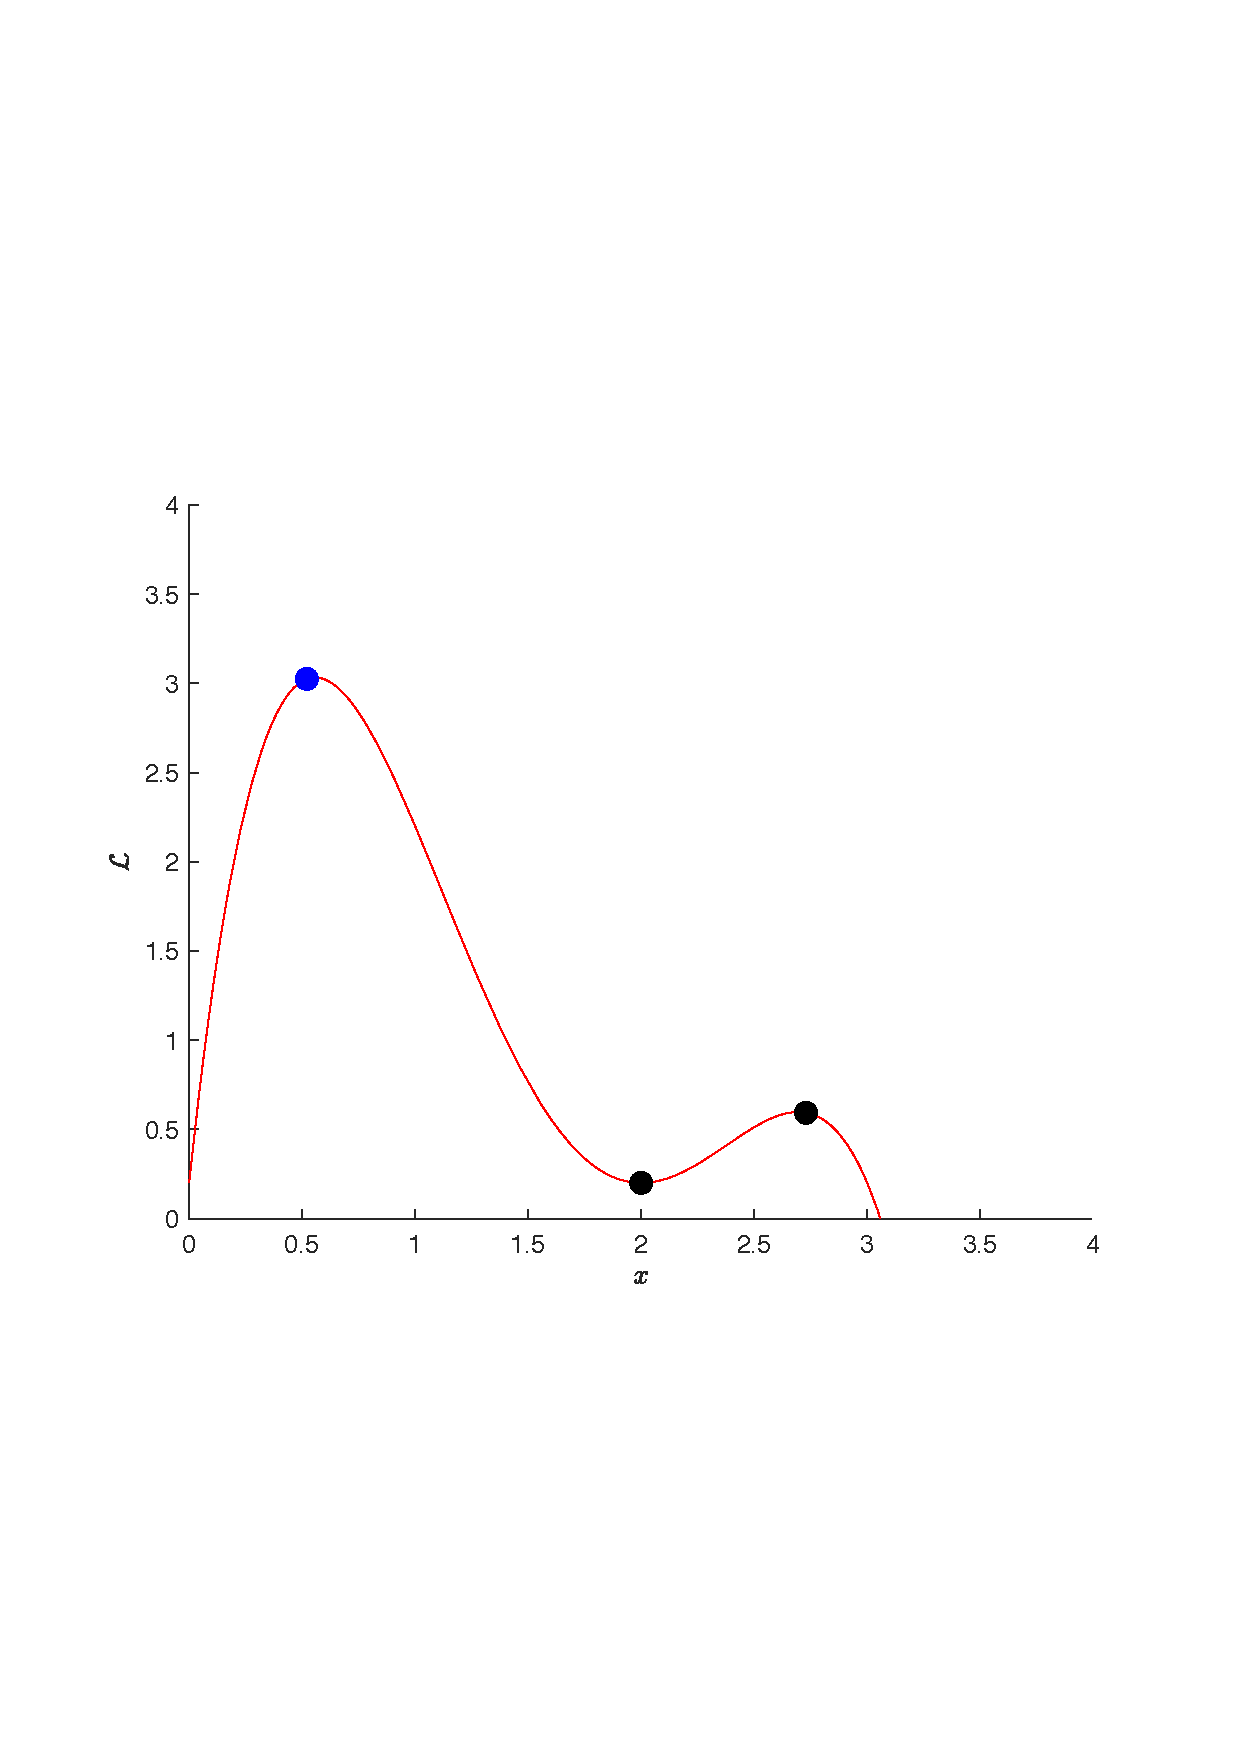
\includegraphics[trim={1.8cm 7.9cm 2.3cm 8cm},clip, width=\textwidth]{figures/likelihoodProblem1}
		\caption*{\emph{a}}
	\end{minipage}
		\begin{minipage}[b]{.499\linewidth}
 		\centering
 		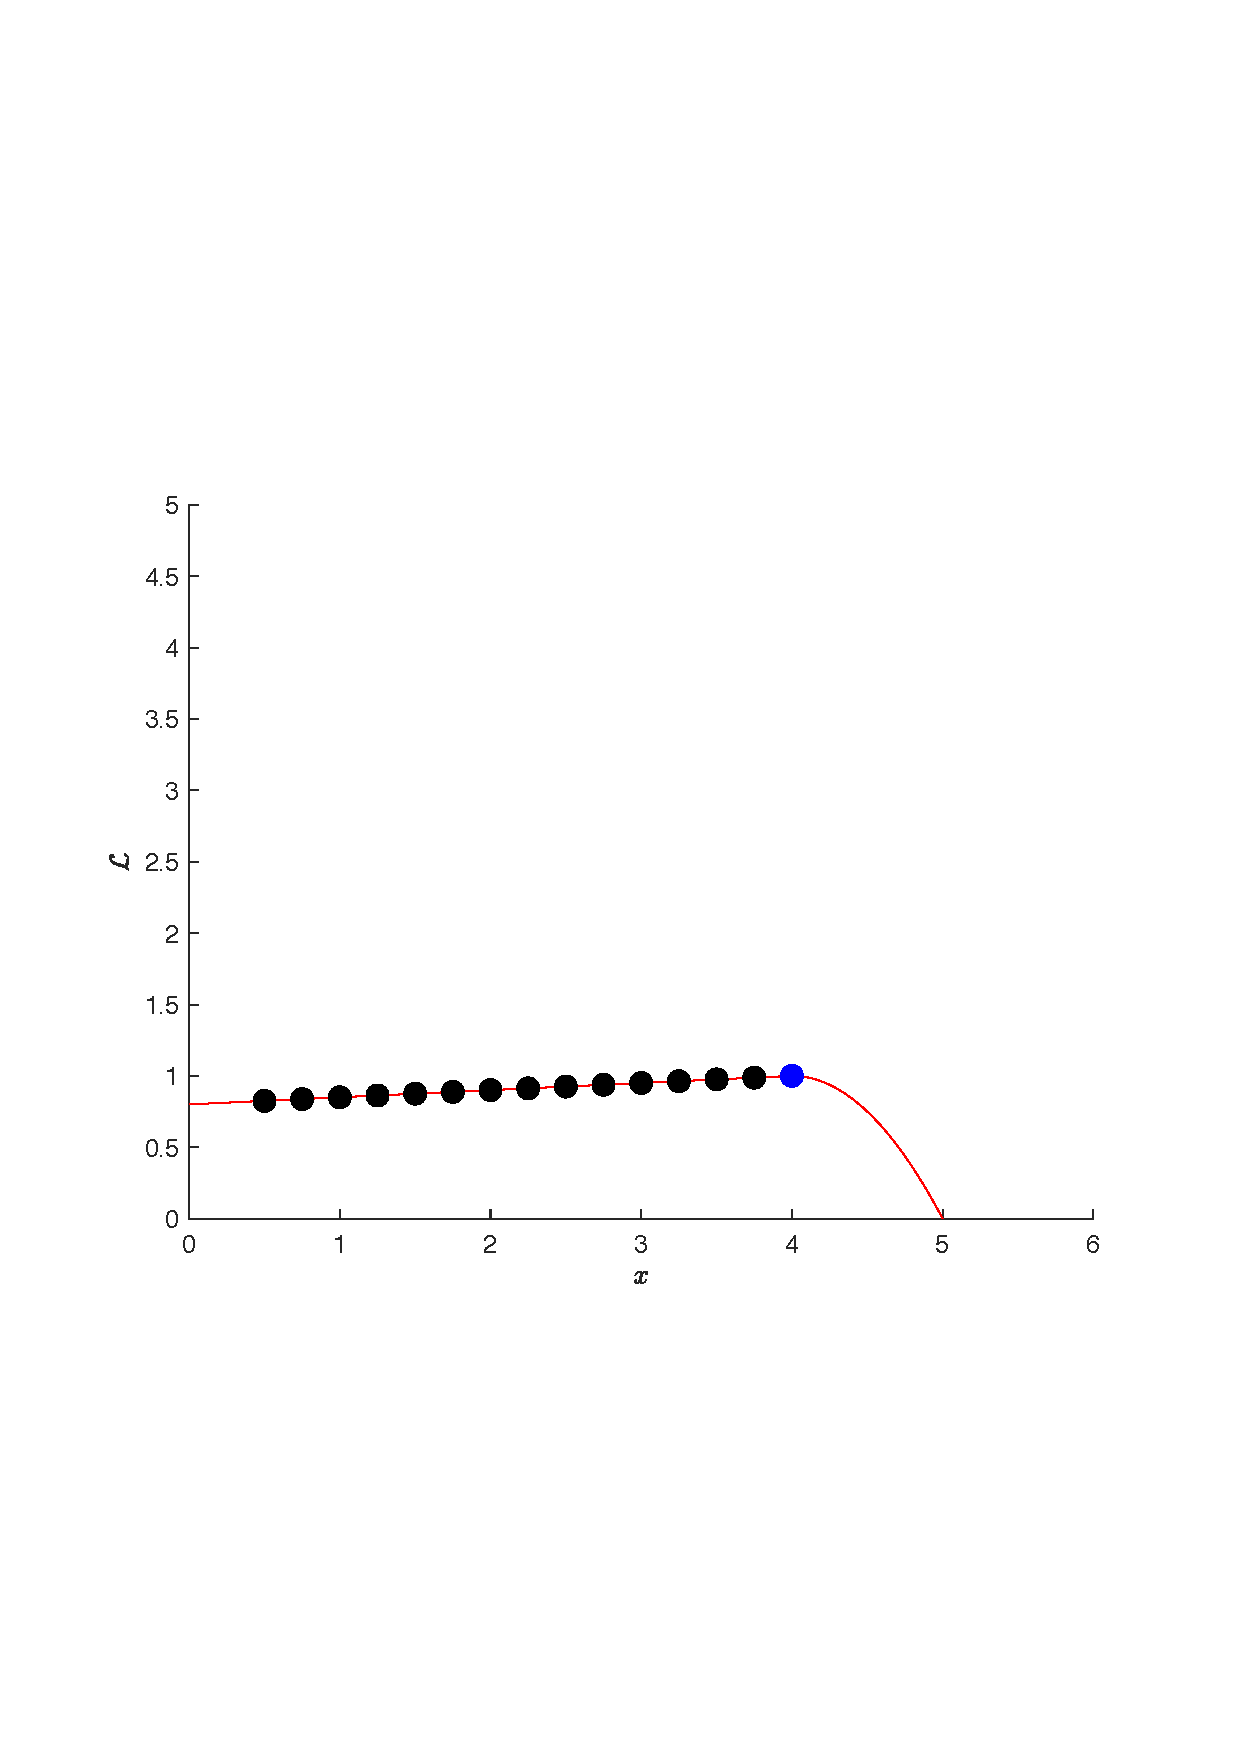
\includegraphics[trim={1.8cm 7.9cm 2.3cm 8cm},clip, width=\textwidth]{figures/likelihoodProblem2}
		\caption*{\emph{b}}
	\end{minipage}
		\begin{minipage}[b]{.499\linewidth}
 		\centering
 		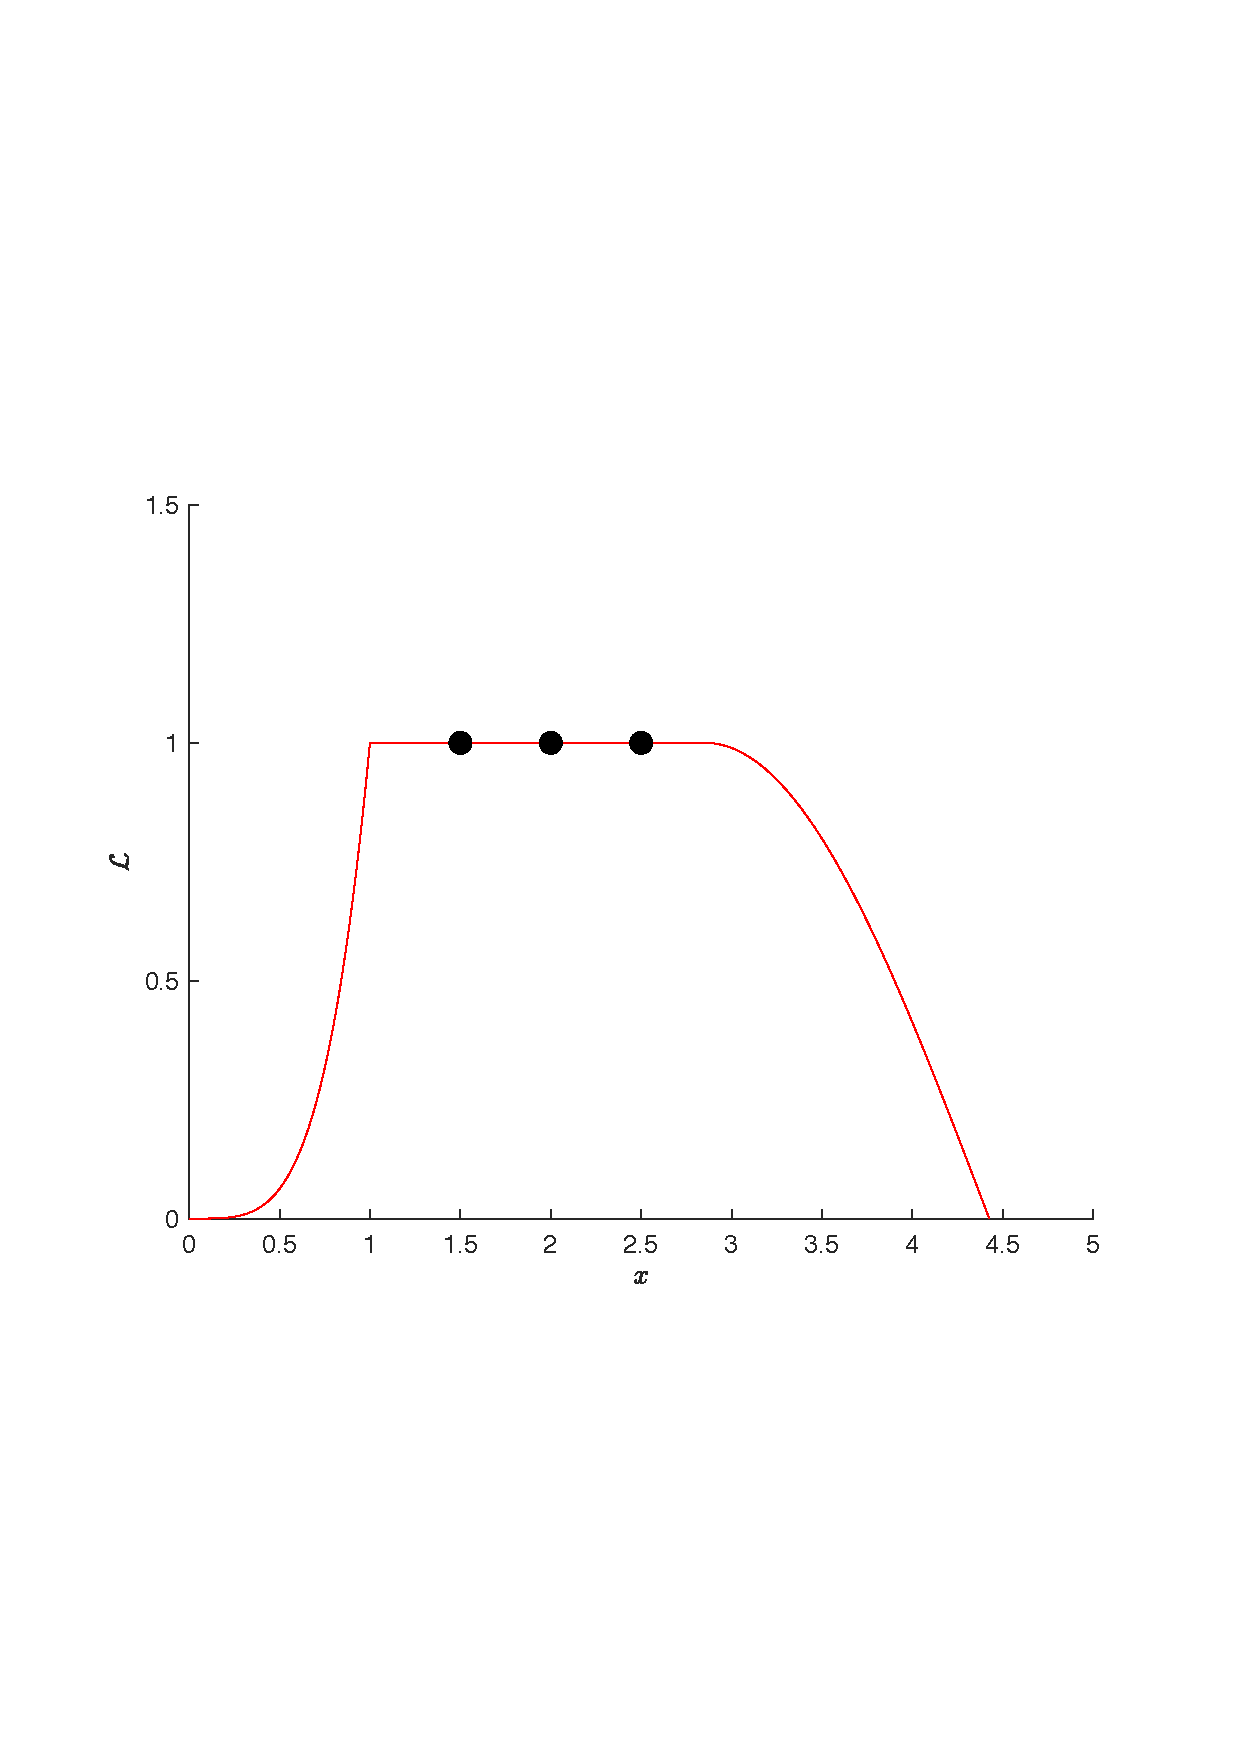
\includegraphics[trim={1.8cm 7.9cm 2.3cm 8cm},clip, width=\textwidth]{figures/likelihoodProblem3}
		\caption*{\emph{c}}
	\end{minipage}
		\begin{minipage}[b]{.499\linewidth}
 		\centering
 		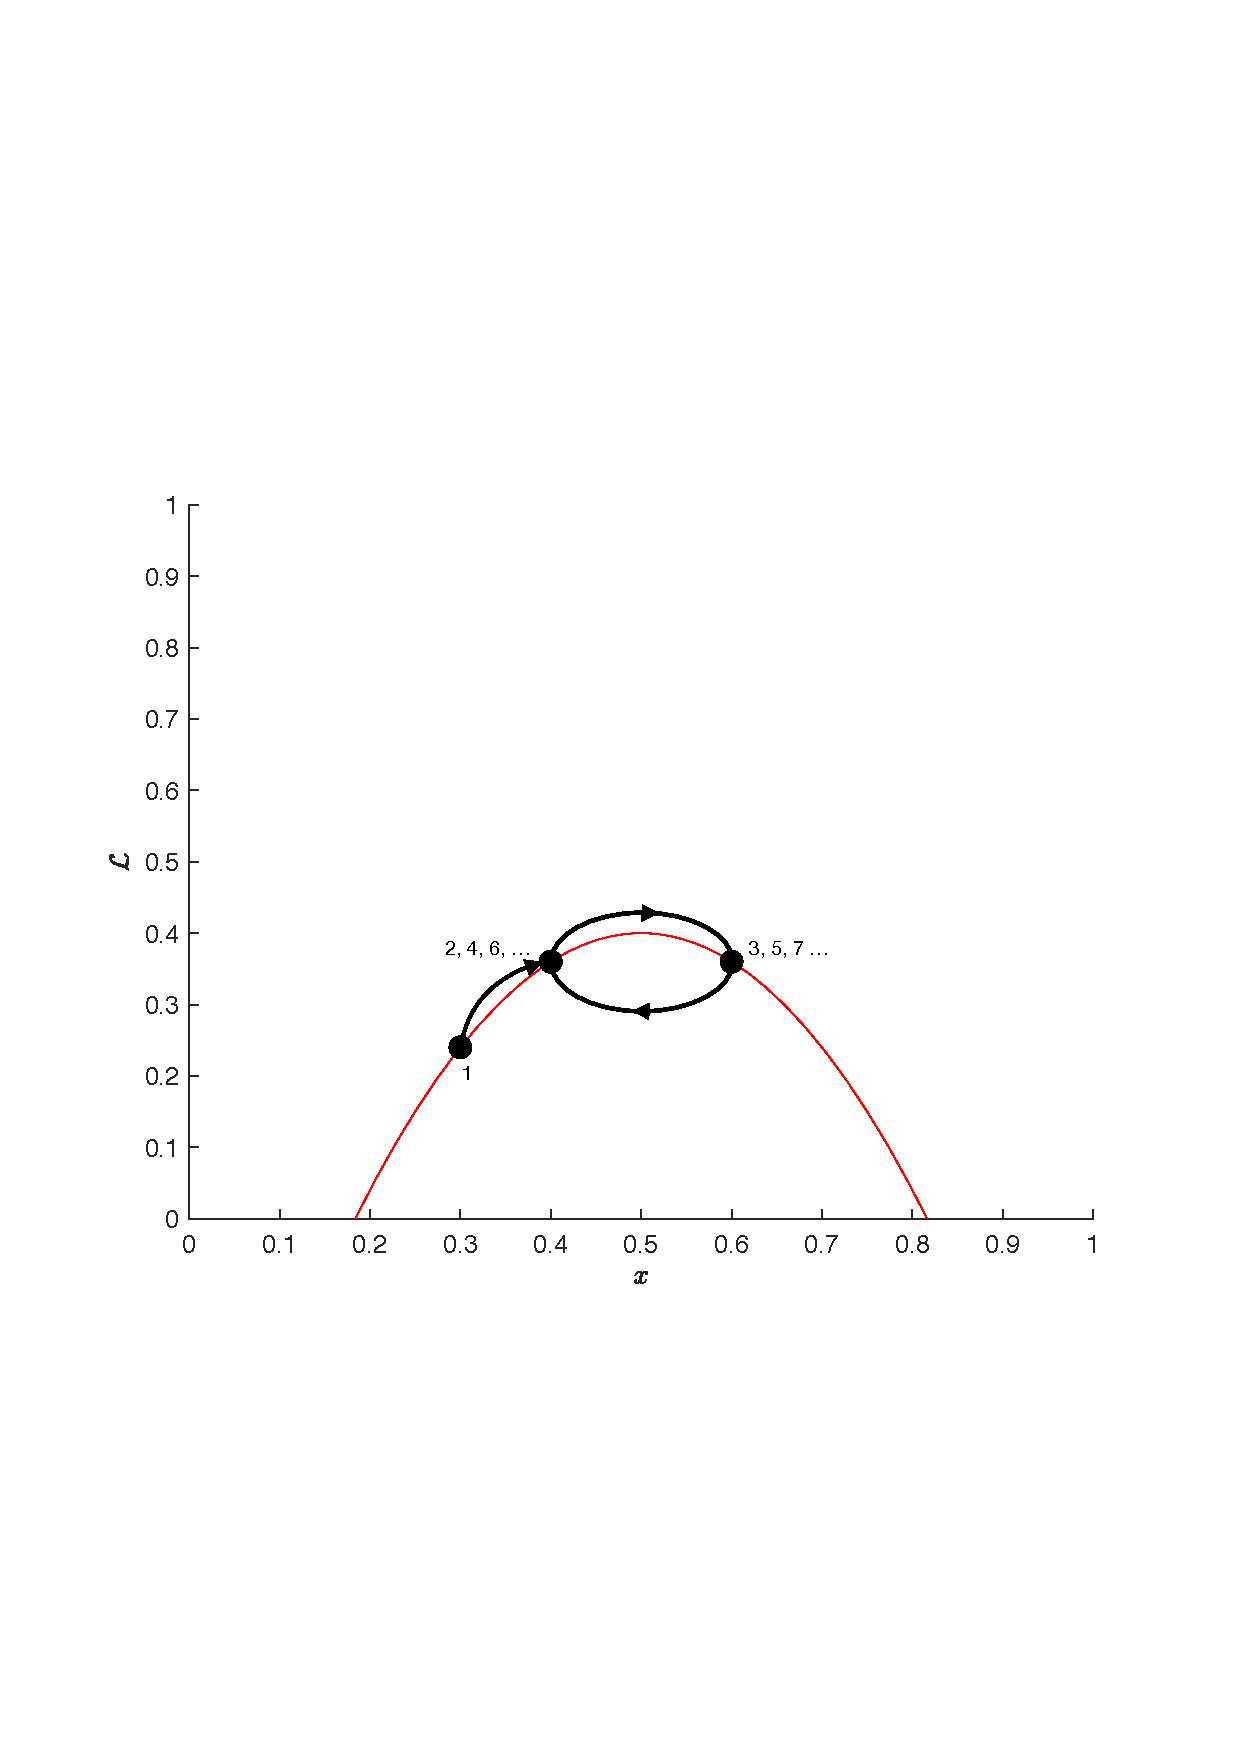
\includegraphics[trim={1.8cm 7.9cm 2.3cm 8cm},clip, width=\textwidth]{figures/likelihoodProblem4}
		\caption*{\emph{d}}
	\end{minipage}
	\caption{\emph{Examples of the problems that may arise with certain likelihood functions.\newline\\
	a: The black estimators are found by setting the score to 0, but they are not the global maximum of the likelihood and are therefore not ML estimators. Only the blue estimator is a good ML estimator.\newline\\
	b: If an iterative algorithm is used to find the ML estimator, it may need a lot of iterations (black) before finding the ML estimator (blue). This is especially true for flatter likelihoods.\newline\\
	c: If the likelihood is constant on some parameter range, the estimators found are not unique and no good ML estimator will be found (in that range).\newline\\
	d: If the iteration step size is not appropriate an iterative algorithm may systematically overshoot the ML estimator and get stuck in a loop, failing to converge.}}
	\label{fig:likelihoodProblems}
\end{figure}
\intextsep\skip32




%----------------------------------------------------------------------------
\section{Medical imaging: PET}
Modern medicine relies heavily on different imaging techniques to analyse in a non-invasive way the interior of a patient. The most important techniques are radiography using x-rays, ultrasound, CT (Computed Tomography), MRI (Magnetic Resonance Imaging), SPECT (Single Photon Emission Computed Tomography) and PET (Positron Emission Tomography).\\

PET \cite{petscanners} works by introducing a tracer into the patient. A tracer is a metabolically active biological molecule that emits radiation through radioactive decay. It can be synthesised by replacing a stable constituent atom of a molecule by a radioisotope of the corresponding atom or it can be synthesised by binding a biological molecule to a radioisotope\footnote{Radioisotopes commonly used in PET: \superscript{11}C ($\lambda \approx 20'$), \superscript{13}N ($\lambda \approx 10'$), \superscript{15}O ($\lambda \approx 122"$), \superscript{18}F ($\lambda \approx 110'$), \superscript{68}Ga ($\lambda \approx 68'$), \superscript{82}Rb ($\lambda \approx 1,3'$)}. To reduce the dose of radiation to which the patient will be exposed and to prevent the patient from being radioactive long after the scan, only radioisotopes with a fairly small half-life in the order of minutes to hours are used in nuclear medicine. Tracers that have been approved for use in humans are called radio-pharmaceuticals. The choice of tracer, dose and mode of insertion (intravenous, oral ingestion, inhalation or direct injection) depends on which process, region, organ, ... needs to be examined.\\

A good example of a tracer is fluorodeoxyglucose ( 2-Deoxy-2-[\superscript{18}F]fluoroglucose, FDG). It is a tracer molecule that is analogous to glucose. It is often used in oncology to map the growth and distribution of cancer cells through the patient as glucose levels build up in tumours. As such, localised extreme concentrations (in unusual places) in the patient indicate tumour(s). 

To proceed, FDG is injected intravenously whereafter it rapidly spreads through the patient's body and builds up in cells with a high glucose demand.

\begin{figure}[h]
	\begin{minipage}[t]{0.5\textwidth}
		\phantom{Some text}
		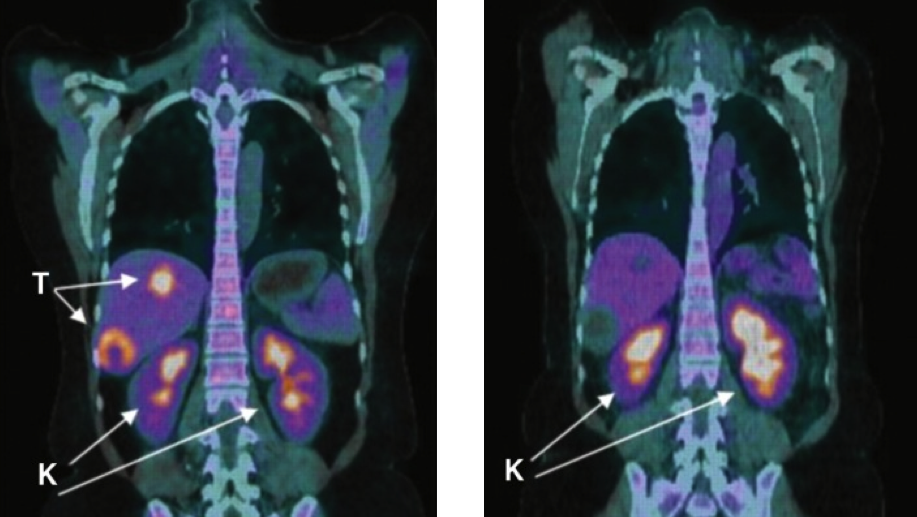
\includegraphics[width=\linewidth]{figures/cancer}
  	\end{minipage}\hfill
  	\begin{minipage}[t]{0.45\textwidth}
    	\caption{\emph{FDG can be used as a tracer in oncology. On the left the extreme and local buildup of FDG in the liver at location T indicates a tumour. On the right, no buildup of FDG can be seen at T. This indicates that the patient responded well to the treatment. The buildup of FDG at K, the kidneys is normal.}}
  	\end{minipage}
\end{figure}




%----------------------------------------------------------------------------
\subsection{Mechanism and setup}
PET (Positron Emission Tomography) is based on the emission of positrons. The positrons are emitted along with neutrinos by radioisotopes decaying through $\upbeta$\superscript{+} decay: $p^+ \rightarrow n^0 + e^+ + \nu\ (+ E_{kin})$. The emitted positrons have a rest mass of 511 keV and some kinetic energy. The kinetic energy of the positrons has a continuous spectrum, though it can not exceed the total decay energy\footnote{The decay energy is in the order of keV's to a few MeV's, e.g.: $E_{\beta^+}(^{11}C) = 0,96 MeV, E_{\beta^+}(^{18}F) = 0,6335 MeV$} due to conservation of energy. They will travel a short distance, usually not much more than about a millimetre, while loosing some kinetic energy along the path before interacting with a nearby electron.\\

The interaction between an electron and a positron results in the annihilation of both particles. Because the total energy is relatively small, the only possible annihilation process is $e^+ + e^- \rightarrow \gamma + \gamma$ where each $\upgamma$ has an energy of 511 keV due to energy conservation and the $\upgamma$'s will be moving in approximately opposite directions due to momentum conservation.\\

Some of the $\upgamma$'s created by this process will be able to leave the patient's body, while others will be absorbed\footnote{The absorption rate is roughly given by the attenuation coefficient of the human body and is different for the various tissues and compositions of the body. A typical human body absorption rate is  $e^{-0,097 cm^{-1} . 30 cm}$.}. The $\upgamma$'s that leave the body can be detected by dedicated detectors based on scintillation crystals connected to photon-multipliers.\\

For PET the scanner consists of an array of gamma ray detectors, installed on a ring structure around the patient (see fig \ref{fig:pet}). The process of detecting a $\upgamma$ is called a hit. Remark that not all hits can be used in the image reconstruction process for various reasons.\\

Consider the specific scanner setup and the $\upgamma$ creation process through $\upbeta$\superscript{+} decay. If hits are registered more than a few nanoseconds apart (depending on the detector time resolution) then the detected $\upgamma$'s could not have been emitted by the same annihilation process and the hits should therefore not be used.

If the hits occur in detectors too close to each other, the $\upgamma$'s could not have been emitted from within the patient's body because the $\upgamma$'s are emitted approximately collinearly (take for example detector $1$ and detector $3$ in fig \ref{fig:pet}. From the setup it should be clear that the detected $\upgamma$'s could not have been emitted from within the patient and should therefore not be used). 

If an event consists of more or less than exactly two hits (within a few nanoseconds), it is not possible to define a unique line of response (LOR) and the event is useless.

So only events where exactly two hits are registered in a time window of a few nanoseconds, and where the hits are detected by detectors sufficiently far away from each other are used.\\

Important sources of data background in PET are the scattering of photons, which leads to a photon pair being associated to an incorrect LOR and random events where two photons not originating from the same interaction point are associated to a LOR because they arrived in the detector at roughly the same time. An additional source of errors can be the patient's motion. For this reason PET scan times should not be too long (max. 30 minutes) to avoid discomfort leading to patient motion.\\

A typical PET setup is represented in figure \ref{fig:pet}. The image (central grid) is discretised in $j$ pixels (2D) or voxels (3D). This image is treated as a column vector where the elements of the image vector are labeled $x_j$ and $j$ runs from $1$ to $n$.\\

The fundamental detector units in PET are scintillation detectors based on scintillation crystals made of Bismuth Germanium Oxide, Gadolinium Oxyorthosilicate, or Lutetium Oxyorthosilicate. Each detector unit consists of a scintillation crystal which is connected to and read out by a photon multiplier tube or another photodetector such as a silicon photomultiplier or an avalanche photodiode. Detector units are placed in one or possibly multiple rings of about 70 detector units around the image (patient). The current resolution is around 4 mm and is mostly determined by the size of the crystals.

The detectors collect their data as a number of hits. Each detector pair defines a LOR where each LOR is indexed $i$. The data is also treated as a column vector where the elements of the data vector are labeled $y_i$ and run from $1$ to $m$ where the index $i$ runs over all LORs.\\

When a positron (red) is emitted, it will travel for a very short distance before interacting with an electron (blue) and annihilating, resulting in the emission of 2 photons on a line. If two detector units (green) that are not too close to each other detect a photon at the same time, these detector units define a LOR. The problem then is that it is not immediately possible to determine from which pixel the photons originated because they could have originated from any pixel intersected by the LOR\footnote{TOF: Time Of Flight is a technique that relies on extremely fast detectors and data processing to determine the time difference between the arrival of the first and second photon. This makes it possible to at least approximate from which pixel group the photons came ($\pm 10$ cm). This can already be done to some extend and improves the quality of the image reconstruction. To achieve a spatial resolution of 1 mm a detector with a temporal precision of 3 ps would be needed.}. This is what makes PET so difficult.

\begin{figure}[H]
	\begin{minipage}[t]{0.45\textwidth}
		\phantom{Some text}
		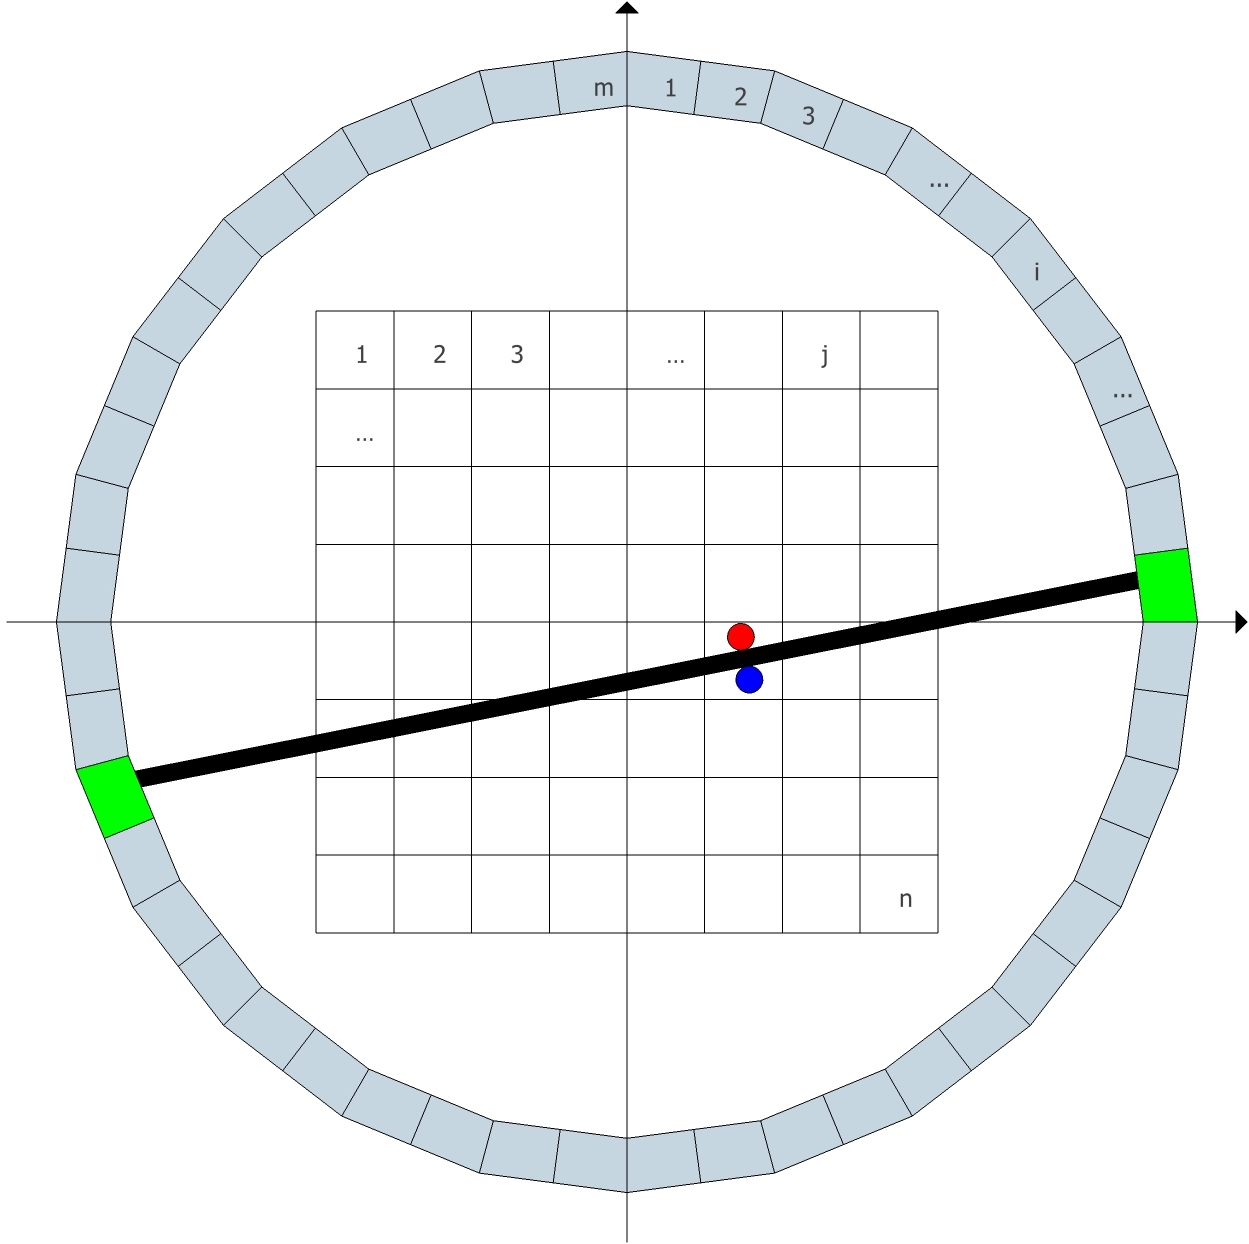
\includegraphics[width=\linewidth]{figures/petSetup}
  	\end{minipage}\hfill
  	\begin{minipage}[t]{0.5\textwidth}
    	\caption{\emph{A typical PET setup in 2D. The pixels and detectors are labeled and numbered, and an event is shown as the annihilation of an electron-positron pair, triggering two detectors along a LOR.}}
		\label{fig:pet}
  	\end{minipage}
\end{figure}




%----------------------------------------------------------------------------
\subsection{Typical values}
\label{sect:typicalvalues}
Ideally a PET-scan should use high tracer doses and long scan times to collect more data, which in turn allows for a more precise reconstruction. Unfortunately in real situations it is not possible to use high doses nor is it possible to scan for too long.\\

For medical PET-scans, the scan time ranges from 15 to 30 minutes. Longer scan times are not desirable because patient motion is expected to increase due to the discomfort of having to lie perfectly still for a longer period of time. This introduces additional errors, which cancel the benefits of collecting data for a longer period of time.\\ 

Due to health concerns associated with radiation and its cancerogenic nature, the tracer dose injected into a patient can not be too high. The exact safe upper limit depends on the isotope being used and its half-life, as well as the tracer's biological half-life. For FDG a typical dose is about 370 MBq (=10 mCi ).\\

With these numbers, it is possible to compute the number of photons expected to be detected. A tracer with an activity of 370 MBq undergoes 37 x 10\superscript{7} disintegrations/second. If the measuring time is only 5 minutes, this amounts to a total of 1,11 x 10\superscript{11} disintegrations, and just as much photon pairs. Due to attenuation and absorption in the patient, not all of those photon pairs will escape the patient. A typical attenuation coefficient is $e^{-0,097 cm^{-1} . 30 cm}$ so only 6,12 x 10\superscript{9} photon pairs escape the patient. Accounting for the geometry of the setup and efficiency of the detector introduces a factor 0,02. Only 1,22 x 10\superscript{8} photon pairs are detected. A  scanner has about (1/2) x 10\superscript{9} lines of response (detector pairs), which gives only 0,25 photon pairs per line of response.\\

This is just an indication of the order of magnitude that the data may have though it does show that for all realistic PET image reconstruction problems the data count is expected to be low. In particular this implies that some asymptotic properties of certain estimators used to reconstruct the image may not be valid for such low data counts. 




%----------------------------------------------------------------------------
%Image reconstruction methods
%----------------------------------------------------------------------------
\chapter{PET image reconstruction methods} \stepcounter{chpt}\setcounter{theorem}{1}
Image reconstruction problems can be presented under different forms and in different contexts, but fundamentally the problem is always the same: an image has to be reconstructed (or estimated), based on indirect and/or incomplete data that may contain significant noise.  	

Several methods exist to solve such problems. Some methods try to give an analytical solution to the problem while other methods use statistical tools to estimate the image.  Statistical methods may implement iterative algorithms to determine the desired estimators.

This chapter will go over some fundamental concepts before presenting several analytical, statistical and iterative image reconstruction methods which are relevant to PET. The next chapters will implement, apply, test and compare the different methods presented in this chapter for different scenario's.




%----------------------------------------------------------------------------
\section{Tomography, projection and backprojection}
The concepts of tomography, projection and backprojection \cite{leastsquare} play a vital role in image reconstruction problems. These concepts will be briefly discussed here for 2D problems.




%----------------------------------------------------------------------------
\subsection{Tomography}
Tomography is the process of imaging a cross section obtained by means of some kind of radiation or wave. In medical imaging a tomography problem is presented as a set of 'projections' of the image from which the image is to be reconstructed.\\

A small example of a tomography problem is the following: suppose there is a 2 x 2 matrix with unknown entries and suppose the row- and column sums are known. Then it is possible to reconstruct the matrix. The matrix elements are of course the unknown image pixels and the row- and column sums are the projections of the elements along 4 LORs. In this case the problem is almost trivial, but it gives some feeling about what a tomography problem is. Remark that even for a problem as simple as this one the solution is not unique. Measuring a third projection at a 45 degrees angle between the two existing projections would allow determining which solution corresponds to the real image. 

\begin{minipage}[t][][c]{.30\textwidth}
\centering
\begin{table}[H]
\centering
\begin{tabular}{c|cc|ccc}
\cline{1-4} \cline{6-6}
\multicolumn{2}{|c|}{\multirow{2}{*}{a}} & \multicolumn{2}{c|}{\multirow{2}{*}{b}} & \multicolumn{1}{c|}{} & \multicolumn{1}{c|}{\multirow{2}{*}{4}} \\ \cline{5-5}
\multicolumn{2}{|c|}{}                   & \multicolumn{2}{c|}{}                   & \multicolumn{1}{c|}{} & \multicolumn{1}{c|}{}                   \\ \cline{1-4} \cline{6-6} 
\multicolumn{2}{|c|}{\multirow{2}{*}{c}} & \multicolumn{2}{c|}{\multirow{2}{*}{d}} & \multicolumn{1}{c|}{} & \multicolumn{1}{c|}{\multirow{2}{*}{7}} \\ \cline{5-5}
\multicolumn{2}{|c|}{}                   & \multicolumn{2}{c|}{}                   & \multicolumn{1}{c|}{} & \multicolumn{1}{c|}{}                   \\ \cline{1-4} \cline{6-6} 
                    &                    &                    &                    &                       &                                         \\ \cline{1-4}
\multicolumn{2}{|c|}{6}                  & \multicolumn{2}{c|}{5}                  &                       &                                         \\ \cline{1-4}
\end{tabular}
\end{table}
\end{minipage}%
\begin{minipage}[t][][c]{.30\textwidth}
	\centering
  \begin{align}
  \Rightarrow\ \ \ \ \left\{
  \begin{array}{cc} 
  a+b=4 &  \\ 
  c+d=7 &  \\
  a+c=6 &  \\ 
  b+d=5 &  
  \end{array}\right. \ \ \ \ \Rightarrow\ \ \ \
  \nonumber
  \end{align}
\end{minipage}%s
\begin{minipage}[t][][c]{.30\textwidth}
\begin{table}[H]
\centering
\begin{tabular}{clclclclcl}
\multicolumn{10}{c}{}                                                                                                                                                                                             \\ \cline{1-4} \cline{7-10} 
\multicolumn{2}{|c|}{\multirow{2}{*}{1}} & \multicolumn{2}{c|}{\multirow{2}{*}{3}} & \multicolumn{2}{c|}{\multirow{4}{*}{\ or\ }} & \multicolumn{2}{c|}{\multirow{2}{*}{2}} & \multicolumn{2}{c|}{\multirow{2}{*}{2}} \\
\multicolumn{2}{|c|}{}                   & \multicolumn{2}{c|}{}                   & \multicolumn{2}{c|}{}                    & \multicolumn{2}{c|}{}                   & \multicolumn{2}{c|}{}                   \\ \cline{1-4} \cline{7-10} 
\multicolumn{2}{|c|}{\multirow{2}{*}{5}} & \multicolumn{2}{c|}{\multirow{2}{*}{2}} & \multicolumn{2}{c|}{}                    & \multicolumn{2}{c|}{\multirow{2}{*}{4}} & \multicolumn{2}{c|}{\multirow{2}{*}{3}} \\
\multicolumn{2}{|c|}{}                   & \multicolumn{2}{c|}{}                   & \multicolumn{2}{c|}{}                    & \multicolumn{2}{c|}{}                   & \multicolumn{2}{c|}{}                   \\ \cline{1-4} \cline{7-10} 
\end{tabular}\end{table}
\end{minipage}





%----------------------------------------------------------------------------
\subsection{Projection}
\setlength\intextsep{0pt}
\begin{wrapfigure}{r}{0.5\textwidth}
\centering
	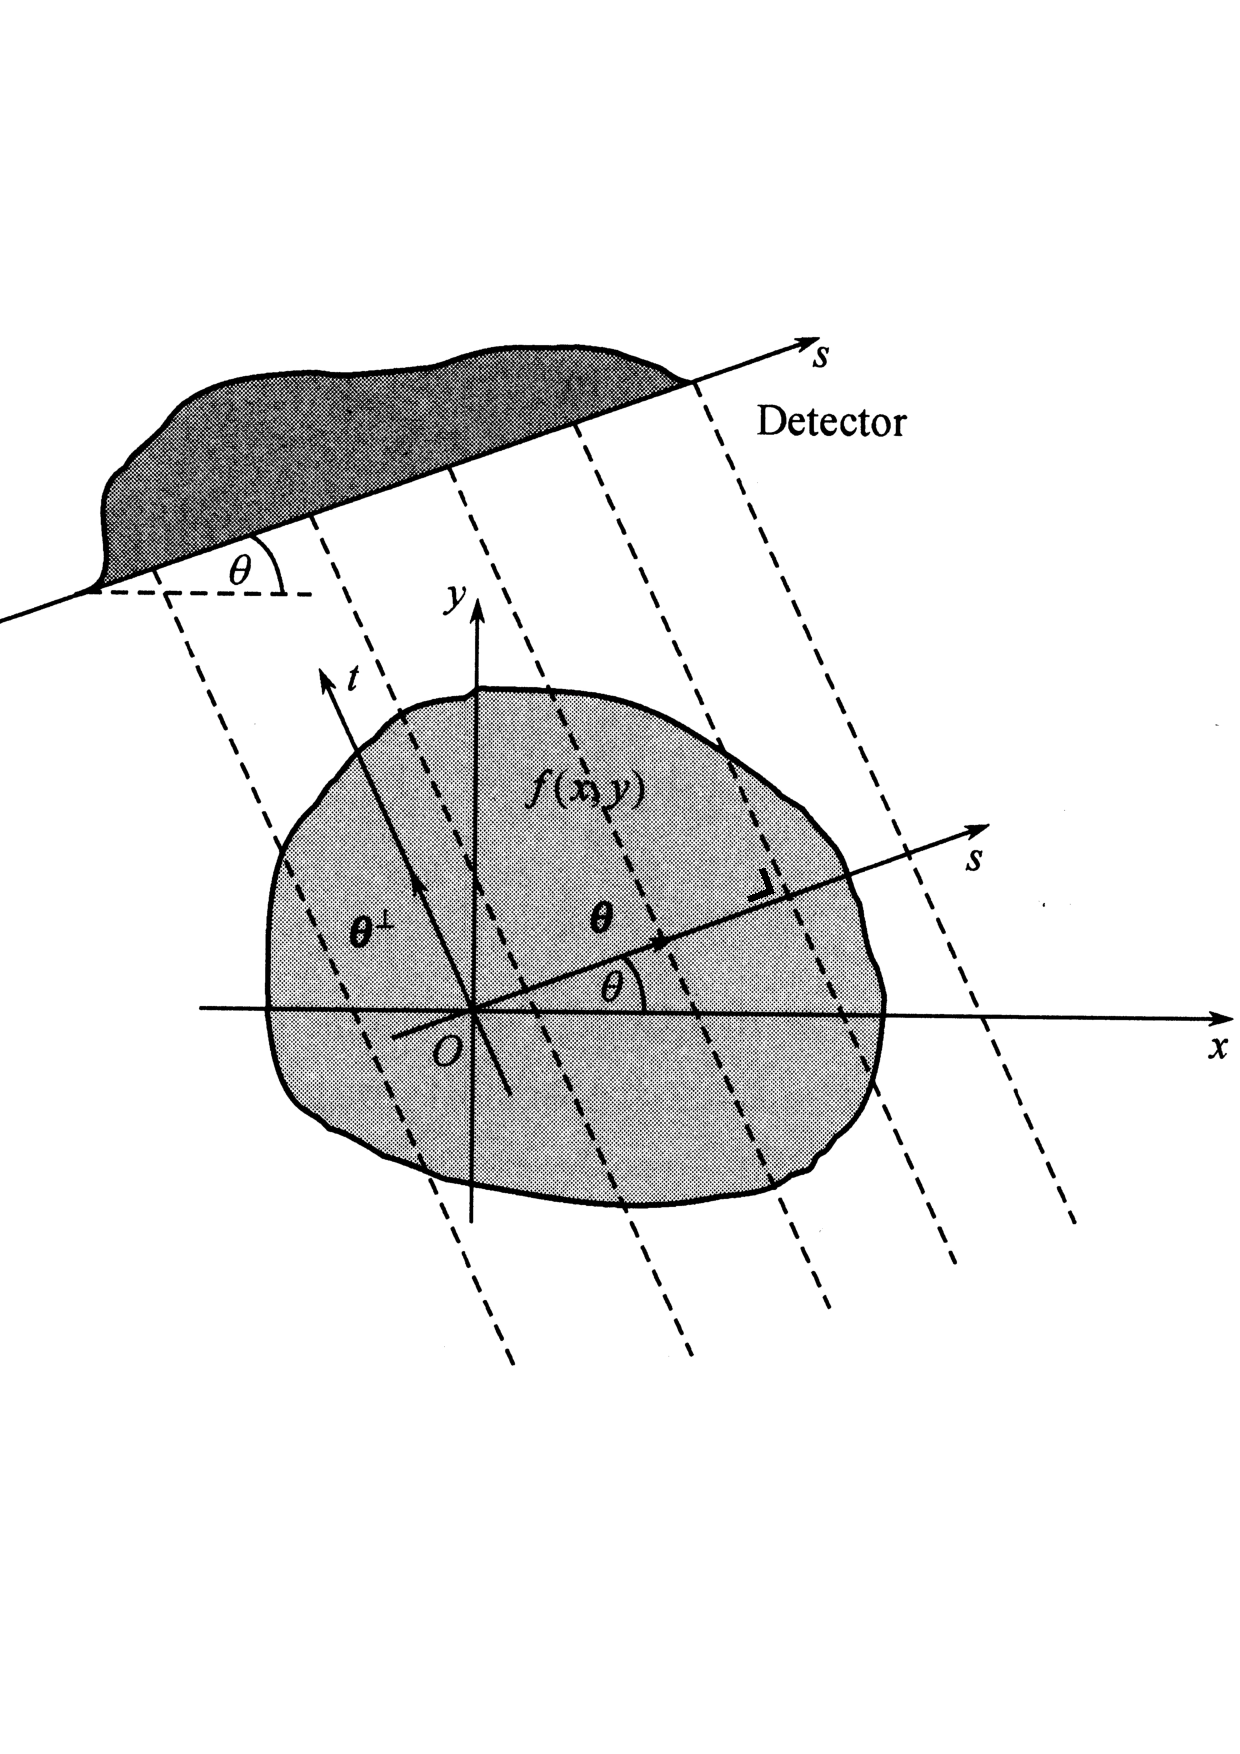
\includegraphics[width=0.4\textwidth]{figures/projection}
	\caption{\emph{The coordinate system for a 2D projection.\\
	Image reprinted from \cite{leastsquare}\\}}
	\label{fig:projection}
\end{wrapfigure}
\intextsep\skip32
The concept of projection (also called ray sum, line integral or Radon transform) has been mentioned in the introduction to tomography. A projection can be seen as a superposition of all contributions along a certain LOR. In the previous example, the projections are the row- and column sums.\\

The coordinate convention is drawn in figure \ref{fig:projection}. The image can be a discrete or continuous distribution of some density function $f(x,y)$ in a cartesian system of axis with coordinates $x$ and $y$. The detector is placed outside the image and revolves around it. The angle between the image's $x$-axis and the detector's $s$-axis is $\theta$. The projection measured by the detector is then a function of the location on the detector $s$ and the angle of the detector $\theta$.\\

Mathematically there is a distinction between the discrete and the continuous case. In the discrete case, the image and the projections are treated as column vectors and the relation between both is given by a matrix, referred to as the system matrix. It is an $m \times n$ matrix which links the image to the projection by modelling the physics and geometry of the scan. The projection is
\begin{align}
	P = AX
	\label{eq:projectionDiscrete}
\end{align} 

In the continuous case, summations are replaced by integrals and the projection takes the following form
\begin{align}
	p(s,\theta) = \int_{-\infty}^{+\infty} \int_{-\infty}^{+\infty} f(x,y) 
	\delta(x\ cos(\theta) + y\ sin(\theta) - s) dxdy
	\label{eq:projection}
\end{align}

with $\delta$ the Dirac $\delta$ function.\\

When the projection is plotted in a 2D plot with on the axis $s$ and $\theta$, the projection of a point source not located at the origin is a sine wave, see fig. \ref{fig:sinogramExample}. Therefore a projection is often referred to as a sinogram. 
\setlength\intextsep{\savedintextsep}
\begin{figure}[H]
	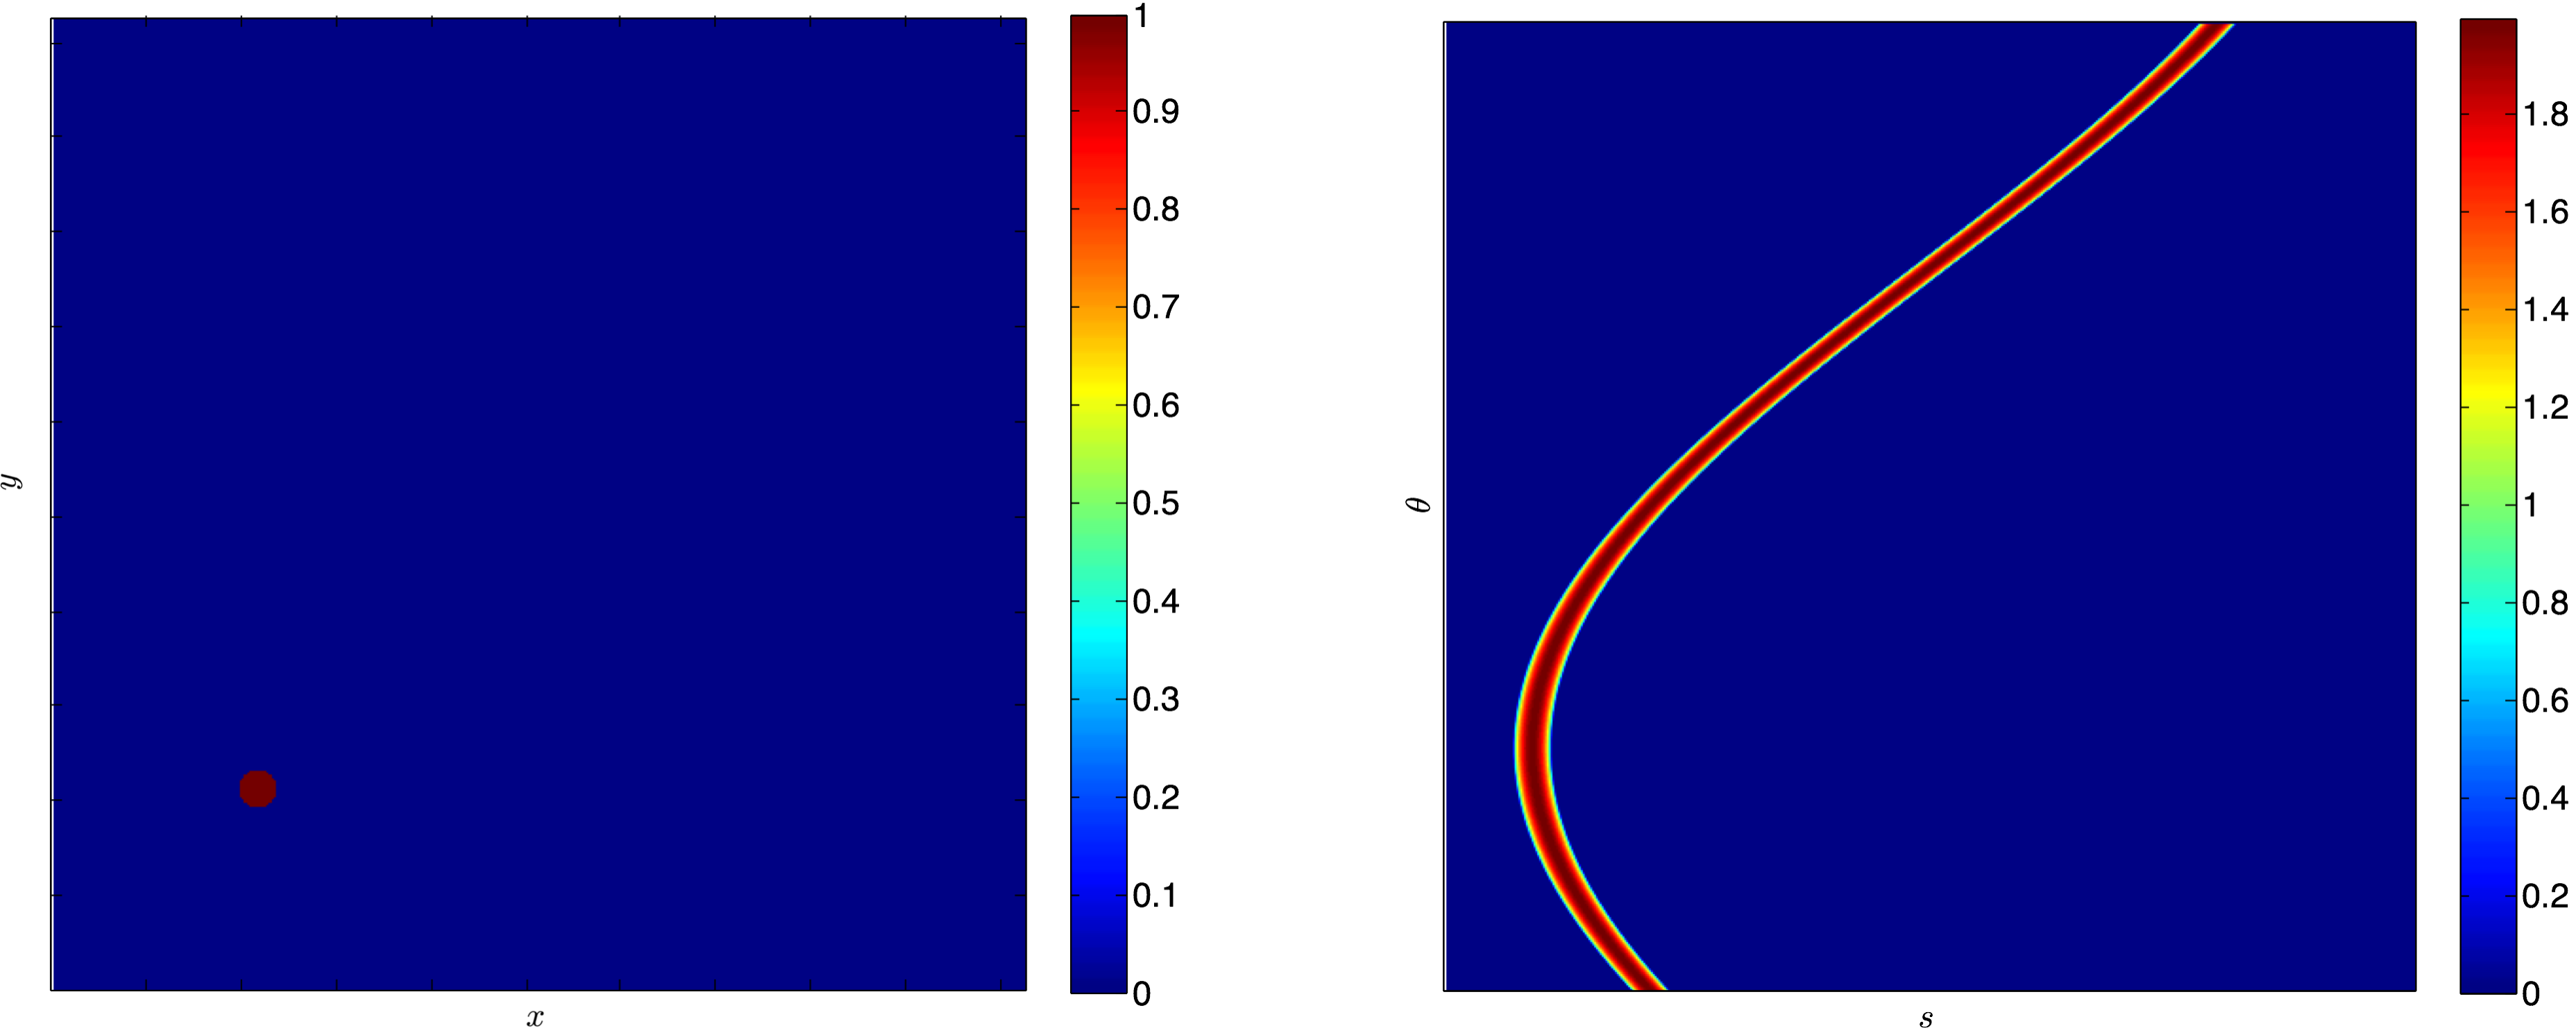
\includegraphics[width=\linewidth]{figures/sinoexample}
	\caption{\emph{A point source not at the origin (left) and its projection (right) which is half of a sine wave.}}
	\label{fig:sinogramExample}
\end{figure}



%----------------------------------------------------------------------------
\subsection{Backprojection}
With the projection operation properly defined, it is possible to define a new operation: backprojection. Whereas projection can be seen as the sum of all contributions along a LOR, backprojection can be seen as the redistribution of the projections along their respective LORs over all pixels (discrete) or points (continuous) along that LOR. Mathematically the backprojection is the adjoint of the projection.

Backprojection is done one view\footnote{A view is the projection of the image in a given direction.} at a time and the final result of the backprojection is the superposition of the backprojections of all individual views.\\

Continuing with the previous example, the backprojected views are (respectively along the horizontal and vertical LOR's) computed and summed to obtain the backprojected image. Remark that this image is not the original image as backprojection is not the inverse of projection.
\setlength\intextsep{\savedintextsep}
\begin{table}[H]
\centering
\begin{tabular}{|c|l|c|l|cc|c|l|c|l|cl|c|l|c|l|}
\cline{1-4} \cline{7-10} \cline{13-16}
\multicolumn{2}{|c|}{\multirow{2}{*}{4}} & \multicolumn{2}{c|}{\multirow{2}{*}{4}} &                    &                    & \multicolumn{2}{c|}{\multirow{2}{*}{6}} & \multicolumn{2}{c|}{\multirow{2}{*}{5}} &                      & \multicolumn{1}{c|}{} & \multicolumn{2}{c|}{\multirow{2}{*}{10}} & \multicolumn{2}{c|}{\multirow{2}{*}{9}}  \\
\multicolumn{2}{|c|}{}                   & \multicolumn{2}{c|}{}                   & \multicolumn{2}{c|}{\multirow{2}{*}{+}} & \multicolumn{2}{c|}{}                   & \multicolumn{2}{c|}{}                   & \multicolumn{2}{c|}{\multirow{2}{*}{=}}      & \multicolumn{2}{c|}{}                    & \multicolumn{2}{c|}{}                    \\ \cline{1-4} \cline{7-10} \cline{13-16} 
\multicolumn{2}{|c|}{\multirow{2}{*}{7}} & \multicolumn{2}{c|}{\multirow{2}{*}{7}} & \multicolumn{2}{c|}{}                   & \multicolumn{2}{c|}{\multirow{2}{*}{6}} & \multicolumn{2}{c|}{\multirow{2}{*}{5}} & \multicolumn{2}{c|}{}                        & \multicolumn{2}{c|}{\multirow{2}{*}{13}} & \multicolumn{2}{c|}{\multirow{2}{*}{12}} \\
\multicolumn{2}{|c|}{}                   & \multicolumn{2}{c|}{}                   &                    &                    & \multicolumn{2}{c|}{}                   & \multicolumn{2}{c|}{}                   & \multicolumn{1}{l}{} &                       & \multicolumn{2}{c|}{}                    & \multicolumn{2}{c|}{}                    \\ \cline{1-4} \cline{7-10} \cline{13-16} 
\end{tabular}
\end{table}

Backprojection is the adjoint of projection so in the discrete case backprojection is
\begin{align}
	B = A^TP
\end{align}
	
and in the continuous case
\begin{align}
	b(x,y) = \int_0^{\pi} p(s,\theta)\mid_{s=x\ cos(\theta)+ y\ sin(\theta)} d\theta
\end{align}




%----------------------------------------------------------------------------
\section{Analytical reconstruction}
Analytical image reconstruction methods used to be very popular due to their computational ease and because of their numerical stability. The only analytical reconstruction method that will be discussed is filtered backprojection (FBP), which will only be discussed because of the insights it may give into the PET image reconstruction problem. It will not be implemented in the following chapters.



%----------------------------------------------------------------------------
\subsection{Filtered backprojection}
Filtered backprojection used to be a popular image reconstruction method before the (widespread) availability of capable computers allowed the use of iterative algorithms in statistical image reconstruction methods.

The previous section discussed the backprojection operation as being the superposition of all redistribution of the projection along a LOR. Backprojection produces an image that is related to the original image, though the backprojected image appears to be blurred compared to the original. This blurring can be removed by applying a high-pass filter\footnote{A high-pass filter reduces or eliminates small frequency components.}. The main disadvantage of FBP is that the high-pass filter does reduce blurring but it also enhances high-frequency noise!
\begin{figure}[H]
  	\begin{minipage}[t]{0.45\textwidth}
    	\caption{\emph{The (conceptual) process of reconstructing the image of a point source using FBP.\\ \\
	a) The point source is projected in multiple directions, creating multiple views.\\ \\
	b) The projection of one view is backprojected.\\ \\
	c) The superposition of a few views creates a spike at the point source's location.\\ \\
	d) The complete backprojection is as expected the point source, but unfortunately it is blurred due to the naive redistribution of the projection data.\\ \\
	e+f) Adding negative 'wings' on the projection data cancels the blurring.}}
		\label{fig:smth}
  	\end{minipage}\hfill
	\begin{minipage}[t]{0.55\textwidth}
		\phantom{Some text}
		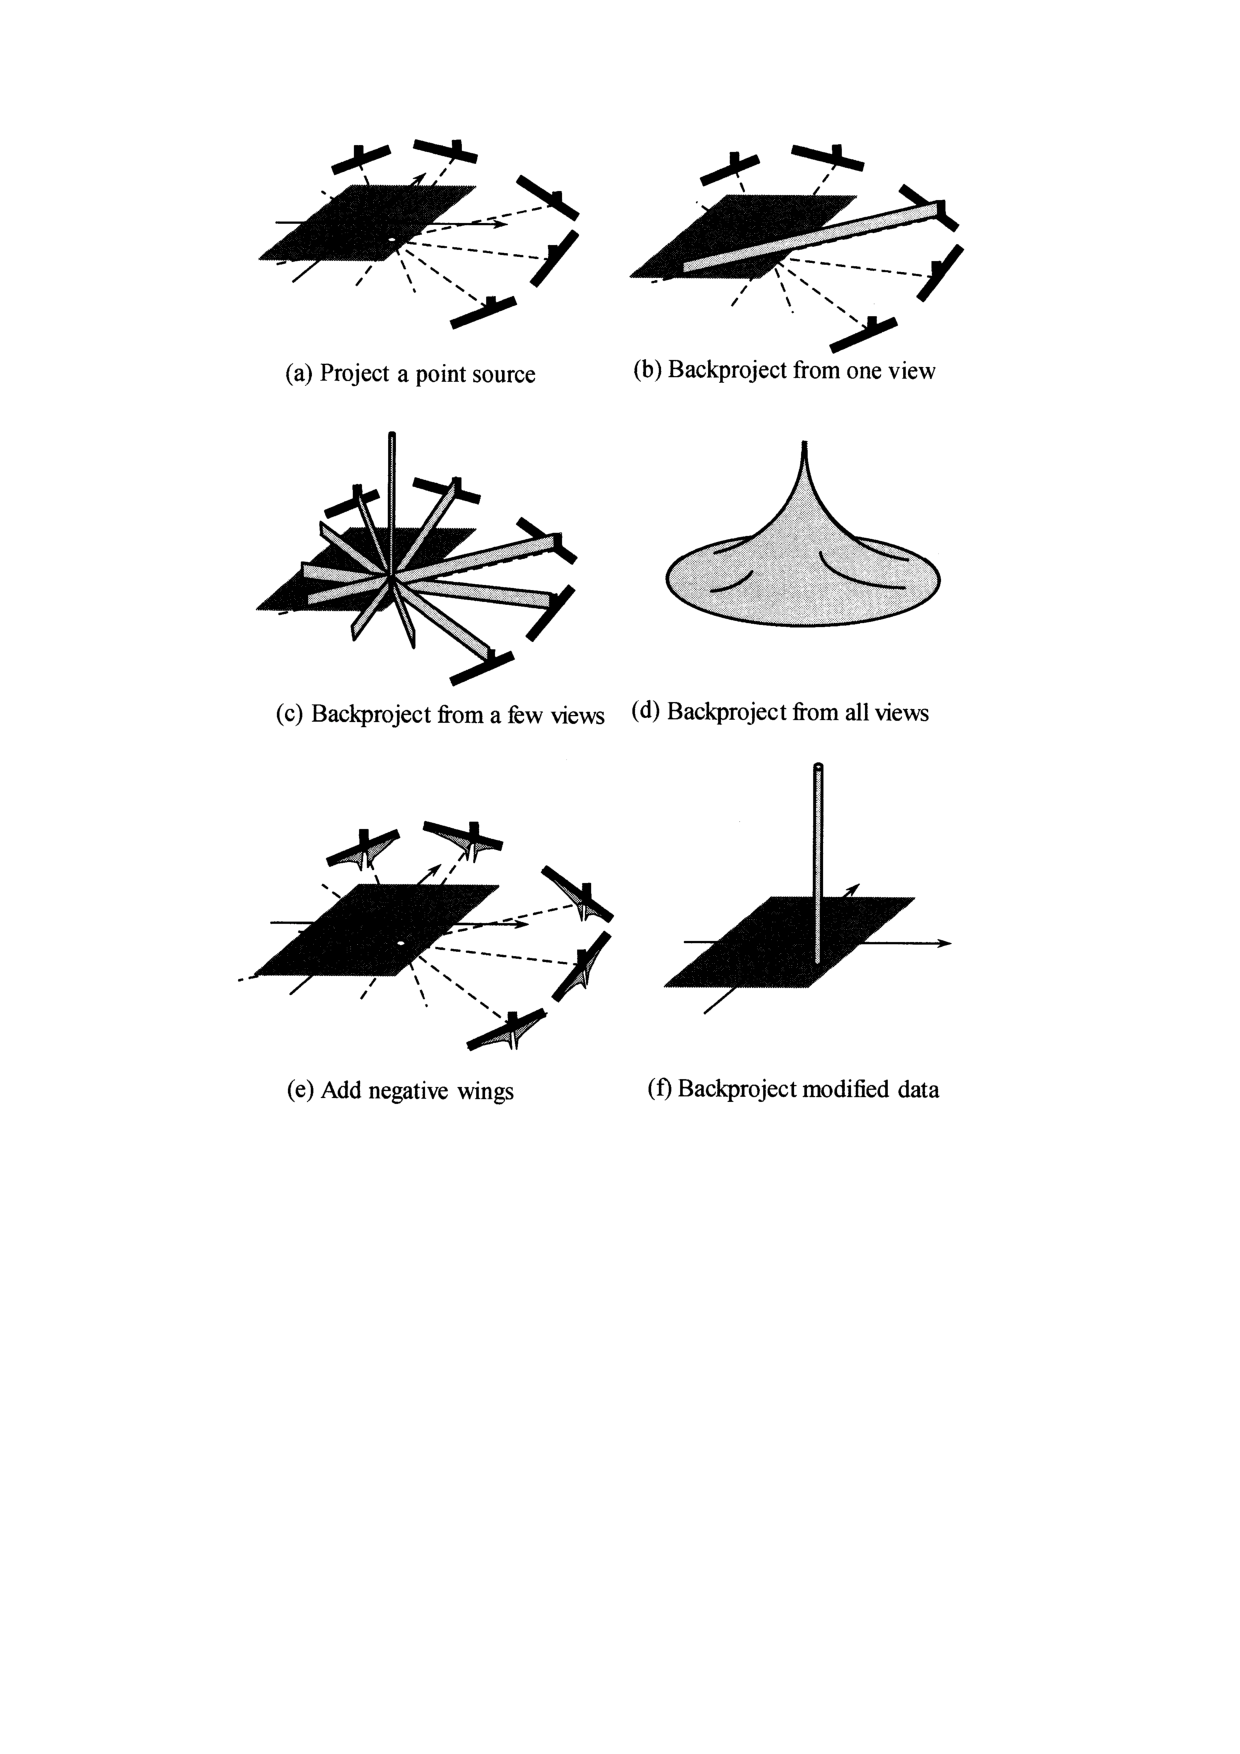
\includegraphics[width=\linewidth]{figures/FBP}
		\caption*{\emph{Image reprinted from \cite{leastsquare}}}
  	\end{minipage}
\end{figure}

FBP is done by applying a filter to the data in the projections. When a spike is detected in the projection, negative wings are added around the spike to the projection. Backprojecting these filtered projections yields sharper results. Mathematically FBP is based on the Fourier transformation. The function $P(\omega, \theta)$ is defined as being the Fourier transform of the projection $p(s, \theta)$: $P(\omega, \theta) = \mathcal{F}(p(s, \theta))(\omega) = \int_{- \infty}^{+ \infty} p(s,\theta)\ e^{-2 \pi i s \omega} ds$.

\subsubsection*{Central slice theorem}
The FBP method can be derived by using the central slice theorem. The central slice theorem as stated in \cite{leastsquare} relates the Fourier transform of the projections with the Fourier transform of the image.

\theorem{
The Fourier transform $P(\omega, \theta)$ of the projections $p(s, \theta)$ of a 2D function $f(x,y)$ is equal to a slice (i.e., a 1D profile) through the origin of the 2D Fourier transform $F(\omega_x, \omega_y)$ of that function which is parallel to the detector, see fig. \ref{fig:fbp2} left and middle.	
\begin{align}
	P(\omega,\theta) = F\big(\omega\ cos(\theta), \omega\ sin(\theta)\big)
\end{align}
}
{
The definition of the 1D Fourier transform is
\begin{align}
	P(\omega) = \int_{-\infty}^{+\infty} p(s) e^{-2\pi i \omega s}ds
\end{align}

where $p(s)$ is defined as \ref{eq:projection}, so this becomes
\begin{align}
	P(\omega, \theta) = \int_{-\infty}^{+\infty}
	\left[ \int_{-\infty}^{+\infty} \int_{-\infty}^{+\infty}
	f(x,y)\ \delta(x\ cos(\theta) + y\ sin(\theta) - s)\ dxdy \right] 
	e^{-2\pi i \omega s}ds
\end{align}

change the order of integration
\begin{align}
	P(\omega, \theta) = \int_{-\infty}^{+\infty}
	\int_{-\infty}^{+\infty} f(x,y)\left[
	\int_{-\infty}^{+\infty} 
	\delta(x\ cos(\theta) + y\ sin(\theta) - s)e^{-2\pi i \omega s}ds
	\right] dxdy
\end{align}

The inner integral over $s$ can easily be found with the properties of the $\delta$ function
\begin{align}
	P(\omega, \theta) &= \int_{-\infty}^{+\infty}
	\int_{-\infty}^{+\infty} f(x,y)\ e^{-2\pi i \omega (x\ cos(\theta) + y\ sin(\theta) - s)} dxdy
	\nonumber\\
	%
	&= \int_{-\infty}^{+\infty} \int_{-\infty}^{+\infty} 
	f(x,y)\ e^{-2\pi i \omega (xu + y\nu)}\big\lvert_{u=\omega\ cos(\theta), \nu=\omega\ sin(\theta)} dxdy
\end{align}

So finally after using the definition of the 2D Fourier transform
\begin{align}
	P(\omega,\theta) = F(\omega_x, \omega_y)\big\lvert_{\omega_x =\omega\ cos(\theta), \omega_y=\omega\ sin(\theta)}
\end{align}
}

\begin{figure}
	\centering
	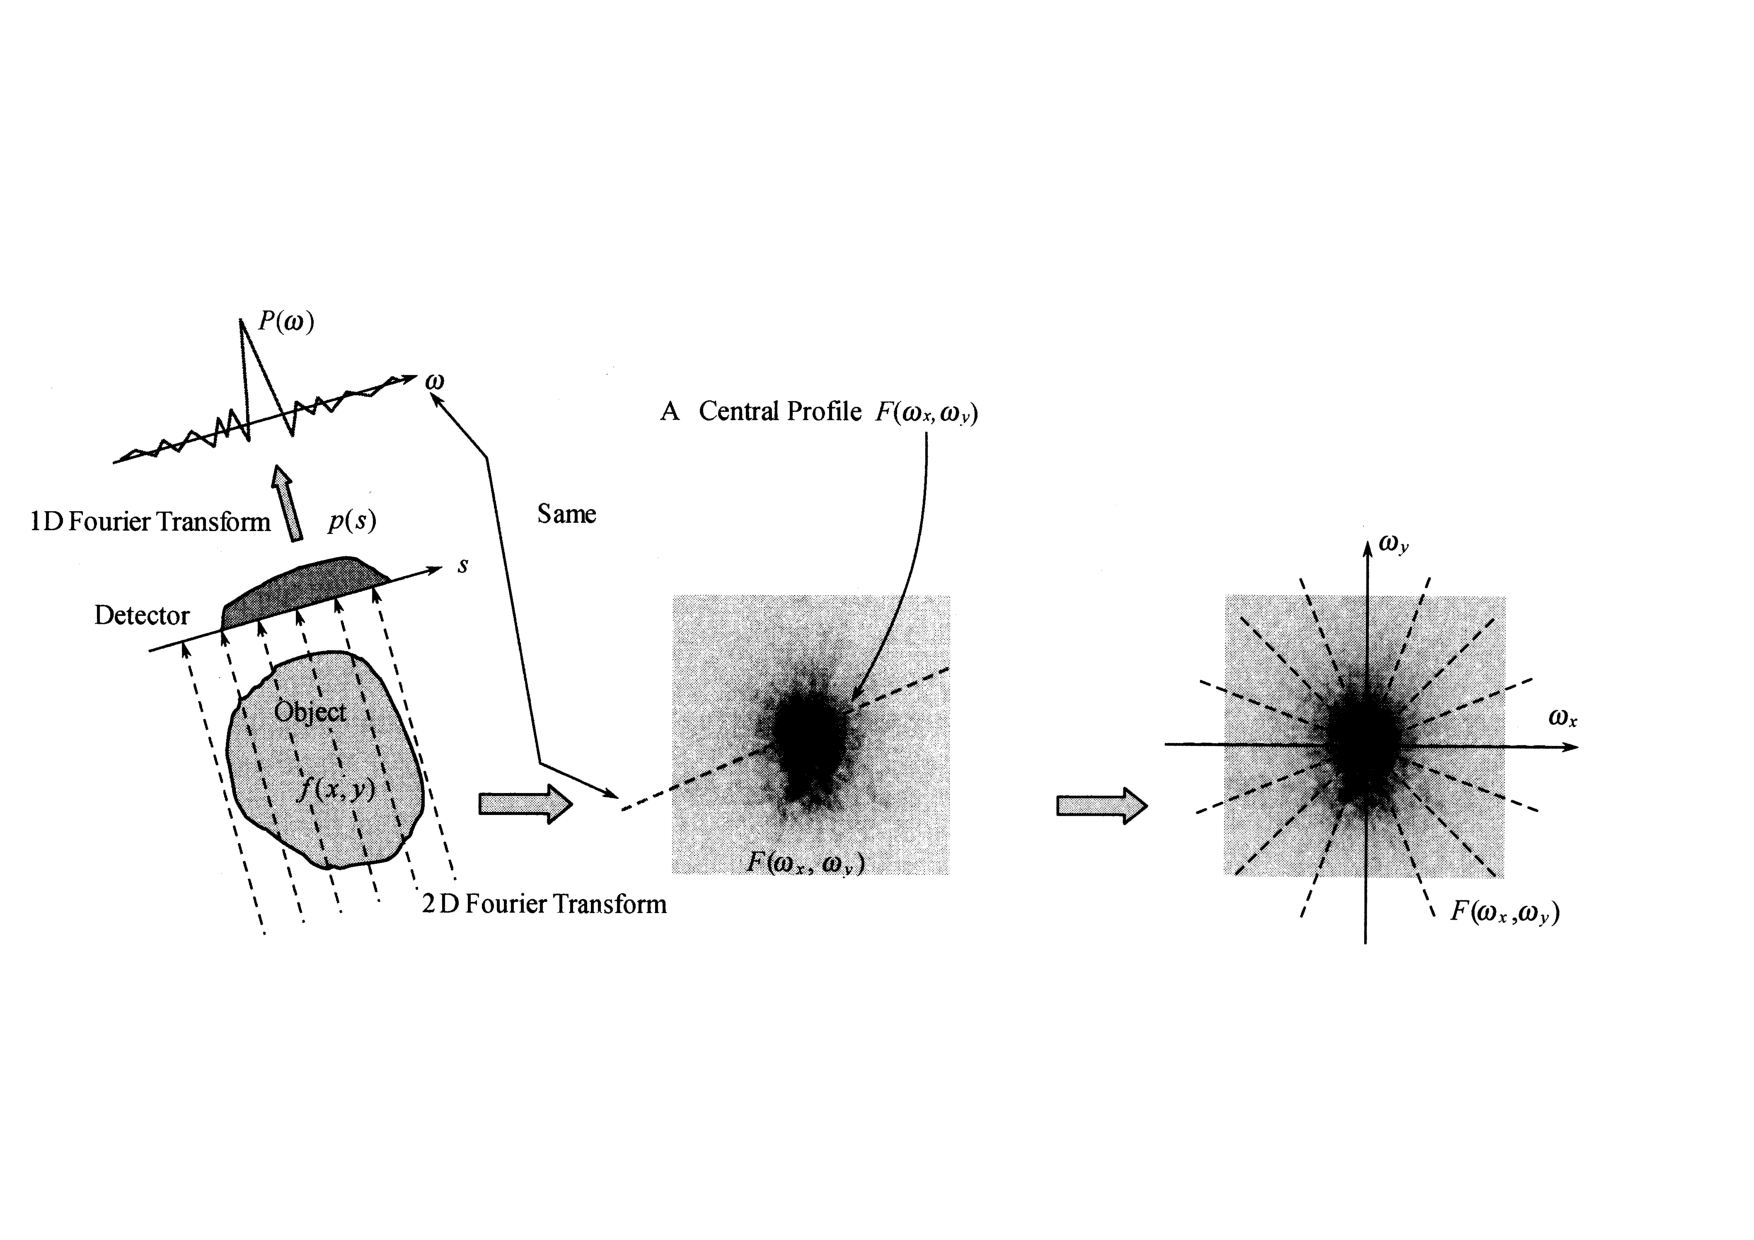
\includegraphics[width=\textwidth]{figures/fbp4}
	\caption{\emph{The central slice theorem. Combining the central slices at all angles $\theta$ reproduces $F(\omega_x,\omega_y)$.\\
	Image reprinted from \cite{leastsquare}}}
	\label{fig:fbp2}
\end{figure}

From the central slice theorem it is clear that the Fourier transform $F(\omega_x,\omega_y)$ of the image $f(x,y)$ can be reconstructed from the projections $p(s,\theta)$ by combining the central slices obtained from the projections at all angles $\theta$, see fig. \ref{fig:fbp2} middle and right.\\

The way in which the image $F(\omega_x, \omega_y)$ is constructed by combining central slices at all angles $\theta$ leads to an interesting problem. The "density of central slices" in $F(\omega_x, \omega_y)$ is not uniform. It is more dense near the origin of the $(\omega_x, \omega_y)$ and decreases radially. This can be seen in fig. \ref{fig:fbp2} right. The central region corresponds to low frequency components. Due to the higher density in the central region, low frequency components are over weighted. Applying the inverse Fourier transform on $F(\omega_x, \omega_y)$ will therefore produce a blurred version of the original image. To produce the original image, the non uniformity must be compensated. The non uniformity is proportional to $1/\sqrt{\omega_x^2 + \omega_y^2}$.

The non-uniformity can be compensated by multiplying the 1D Fourier transform $P(\omega,\theta)$ of the projection data with the filter $|\omega|$. This filter is referred to as the ramp filter due to its shape. By applying the 1D inverse Fourier transform on $|\omega| P(\omega,\theta)$ the filtered projection data is obtained. The original image $f(x,y)$ can then be retrieved by backprojecting the filtered projection data. This procedure is filtered backprojection.\\

The FBP algorithm is
\begin{enumerate}
	\item Obtain the projections $p(s,\theta)$.
	
	\item Find the Fourier transform of the projections $P(\omega, \theta) = \mathcal{F}(p(s,\theta)(\omega,\theta)$.
	
	\item Apply the ramp filter on the transformed projections: $Q(\omega, \theta) = |\omega|\ P(\omega, \theta)$.
	
	\item Retrieve the filtered projection data with the inverse Fourier transformation: $q(s,\theta) = \mathcal{F}^{-1}(Q(\omega, \theta))(s,\theta)$
	
	\item Reconstruct the desired image by backprojecting all the filtered projections.
	
\end{enumerate}




%----------------------------------------------------------------------------
\section{Statistical reconstruction}
Statistical reconstruction methods such as maximum likelihood estimation or least squares estimation can be used to solve PET image reconstruction problems. These methods are based on the statistical properties of the problem. To use statistical reconstruction methods, the continuous image must be discretised into pixels and represented as a matrix where each matrix entry is the activity in the corresponding pixel. The various reconstruction methods then aim to determine statistical estimators for these activities.

In some simple cases, closed form solutions may exist for the estimators, but often iterative algorithms are used to determine the estimators. This section discusses the general idea of maximum likelihood estimation and least squares estimation in the context of PET. The next section discusses 2 iterative algorithms, MLEM and ISRA, which can determine the maximum likelihood estimators respectively (constrained, non-negative) least squares estimators.



%----------------------------------------------------------------------------
\subsection{Maximum likelihood estimation for PET}
The general idea of estimating parameters by maximising the likelihood has been discussed in detail in the introduction, but there are some subtleties to account for when reconstructing a PET image using the maximum likelihood method.\\

The first step is to derive or model the likelihood. It is defined in eq. \ref{eq:likelihood} as:
\begin{align}
	\mathcal{L}(\vec x \mid \vec y) = 
	\prod_{i=1}^{m} P\left( y_i \mid \vec x \right)
\end{align}

Here $P\left( y_i \mid \vec x \right)$ is the probability density function of detector $i$. The subtlety of PET image reconstruction using the maximum likelihood method is that deriving the likelihood of the data is not obvious. If the likelihood is not exactly known, a reasonable approximation must be made. The detectors' pdfs, and the likelihood, are determined by effects such as the emission process of the $\upgamma$'s, detector dead-time\footnote{The dead-time of a detector is the time directly following a detection during which the detector is not capable of registering a new event.}, attenuation in the patient, detector geometry, flaws and defaults, ... 

The $\upgamma$ emission process through radioactive decay is a Poisson process. If the detector dead-time can be neglected\footnote{In typical PET scans this is the case. Section \ref{sect:typicalvalues} shows that for regular PET scans the data count is expected to be low enough for this assumption to hold.} a reasonable approximation is to assume a Poisson distribution for the data as well. 

Due to the central limit theorem the distribution of the data converges to a Gaussian distribution in the high data count limit. So another possible data distribution that is to be studied is a Gaussian data distribution. This is an approximation to the Poisson distribution which is expected to be accurate in the high data count limit. Unfortunately real PET scans work with low data counts. The question is how the Gaussian approximation performs in this low data count limit.\\

Once the detectors' pdfs are known the likelihood can  be found and maximised to find the ML estimators. This seems simple enough, but as the number of detectors and parameters tend to be large in PET, this method can quickly become complicated.




%----------------------------------------------------------------------------
\subsection{Least squares estimation for PET}
The least squares (LS) method is often used to fit data with a known model. For PET the problem to solve is $Y = AX$, with Y the data or the projections along the LORs, A the system matrix and X the image. This is a linear problem which can be solved by setting up a cost function of the form
\begin{align}
	 \chi^2 = || AX - Y ||^2
\end{align}

The least squares estimators are found by minimising this cost function. For an over-determined problem they are given by \cite{leastsquare}
\begin{align}
	\hat X_{LS} = (A^TA)^{-1}A^TY
\end{align}

If the data covariance is not uniform, the covariance matrix is noted as\\ $V =\ <(Y-AX)(Y-AX)^t>$ and the weighted LS estimators are given by \cite{stat3}
\begin{align}
	\hat X_{LS} = (A^TV^{-1}A)^{-1}A^TV^{-1}Y
\end{align}

assuming V is independent of X. Although conceptually very attractive this closed form solution can not be used because for a real PET problem A is unacceptably large and any method that requires modifications of A such as transposition or even worse inversion is computationally not possible.\\

LS estimators have some useful properties relevant to PET:
\begin{itemize}
	\item It can be proven \cite{proof of ml equal ls} that if the distribution of the data is Gaussian, estimating parameters with a ML method or a LS method yields the same result.

	\item It can be proven \cite{proof of ml equal ls} that any LS estimator is unbiased for a linear problem. 

	\item In general LS estimators can be negative, though in PET both the data $\vec y$ and the system matrix $A$ are non-negative.
\end{itemize}





%----------------------------------------------------------------------------
\section{Iterative algorithms in statistical reconstructions}
Recently statistical image reconstruction methods implementing iterative algorithms have become more popular than analytical reconstruction methods because iterative algorithms offer many advantages. With iterative algorithms it is possible or easier to model different physical and geometrical effects such as attenuation, photon scattering, detector setup, ... This increases the resolution and decreases the noise, which in turn decreases the radiation dose required to achieve a certain image quality. Iterative algorithms work by setting up some sort of objective function for the problem which can then be optimised iteratively.\\


The reason that these methods have only recently become more popular is because they tend to be computationally very expensive. The commercial availability of computers performant enough to run these jobs in a reasonable amount of time is what has allowed iterative statistical image reconstruction methods to break through.




%----------------------------------------------------------------------------
\subsection{MLEM}\label{sec:mlem}
An EM (Expectation-Maximisation) algorithm was first proposed by Dempster and Laird \cite{dempster} and was used by Shepp and Vardi \cite{1982 shepp} to derive the popular MLEM (Maximum Likelihood - Expectation Maximisation) iterative image reconstruction algorithm. 

MLEM converges to a maximum likelihood estimator and the algorithm is derived from an objective function based on two steps. The first step consists of obtaining a new objective function, expressed in terms of an expectation and the second step maximises the new objective function. The MLEM algorithm is expressed as
\begin{align}
	\hat x_{j}^{next} &= \frac{\hat x_{j}^{current}}{\sum_{i=1}^{m}a_{ij}} \sum_{i=1}^{m}a_{ij}
	\frac{y_{i}}{\sum_{p=1}^{n}a_{ip}\hat x_{p}^{current}} \ \ \ \ \ j = 1,\ ...\ ,n
	\label{eq:mlem}
\end{align}

with $\hat x_{j}^{current}$ the current estimate of the activity in pixel $j$, $\hat x_{j}^{next}$ the next (and hopefully better) estimate, $y_i$ the data measured along LOR $i$ and $a_{ij}$ the elements of the $m \times n$ system matrix $A$, which was introduced in eq. \ref{eq:projectionDiscrete}. The derivation of the algorithm is given here.\\

The key realisation of MLEM is that some part of the data only depends on some and not all of the parameters\footnote{Any two detectors define a LOR and the measurements from that LOR only depend on the activities (=parameters) in the pixels along that LOR.}. If it were known what part of the data depends on which parameters, the image reconstruction problem would be easier to solve. The EM part of the algorithm tries to take this into account at each iteration.\\

In a PET-scan, the number of counts detected along the $i$\superscript{th} LOR has a Poisson distribution
\begin{align}
	P(y_i) = \frac{E[y_i]^{y_i} e^{-E[y_i]}}{y_i!}
	\label{eq:g}
\end{align}
	
with $E(y_i) = \sum a_{ij}x_j$. The problem is that it is not possible to determine which count came from which pixel along the LOR. Suppose that it would be possible to sort out all the data in a structure where the contribution from each pixel is known. The photon emission process is Poisson so a measurement $y_i$ is a summation of these Poisson variables. Write
\begin{align}
	y_i = \sum_{j} s_{ij}
\end{align}

with $s_{ij}$ a Poisson variable representing the number of photons detected from a pixel $j$ along a LOR $i$. Each measurement $y_i$ is treated as a summation of such Poisson variables therefore its expected value can be written
\begin{align}
	E[s_{ij}] = a_{ij}x_{j}
\end{align}

The likelihood of the complete (Poisson) dataset is then
\begin{align}
	\mathcal{L} &= \prod_{i,j} \frac{E[s_{ij}]^{s_{ij}} e^{-E[s_{ij}]}}{s_{ij}!} 
	= 
	\prod_{i,j} e^{-a_{ij}x_{j}}\frac{(a_{ij}x_{j})^{s_{ij}}}{s_{ij}!}
\end{align}

Taking the logarithm of this likelihood function yields
\begin{align}
	ln\ \mathcal{L} &= \sum_{i,j} (s_{ij}\ ln(a_{ij}x_j) - a_{ij}x_j) - \sum_{i,j} 
	ln(s_{ij}!)
\end{align}	
	
In this expression, the last term does not contain the parameters $x_j$ and it can be discarded without altering the likelihood maximisation. Call the function to be maximised L which is
\begin{align}
	L = \sum_{i,j} \left( s_{ij}\ ln(a_{ij}x_j) - a_{ij}x_j \right)
\end{align}
	
The first step is the "E (expectation)" step which consists of replacing the unknown $s_{ij}$'s by their expected values, given the measurements $y_i$ and the current estimates of the parameters $\hat{\vec{x}}$. With these, the expected value of $s_{ij}$ is
\begin{align} 
	E[s_{ij} \mid y_i, \hat{\vec{x}}^{current}] = \frac{a_{ij}\hat x_{j}^{current}}{\sum_p a_{ip}\hat x_{p}^{current}}y_i
\end{align}

The function to be maximised then becomes
\begin{align}
	E[L \mid \vec y, \hat{\vec{x}}^{current}] = \sum_{i,j} \left( 
	\frac{a_{ij}\hat x_{j}^{current}}{\sum_p a_{ip}\hat x_{p}^{current}}y_i\ ln(a_{ij}x_{j}^{}) - a_{ij} x_j
	\right)
\end{align}

The "M (maximisation)" step consists of maximising this new function. To do so, the derivative is taken with respect to the estimation parameters $\hat{\vec{x}}$ and the derivatives are set to zero
\begin{align}
	\frac{\partial E[L \mid \vec y,\hat{\vec{x}}^{current}]}{\partial x_j} 
	&= 
	\sum_{i} \left(
	\frac{a_{ij} \hat x_{j}^{current}}{\sum_{p} a_{ip}\hat x_{p}^{current}} y_{i} 
	\frac{a_{ij}}{a_{ij}x_{j}} - a_{ij}
	\right)
	\nonumber
	\\
	%
	&= \frac{1}{x_j} 
	\sum_{i} \frac{a_{ij} \hat x_{j}^{current}}{\sum_{p} a_{ip}\hat x_{p}^{current}} y_{i}
	- \sum_{i}a_{ij}
	\nonumber
	\\
	%
	&= 0
\end{align}

Solving for $x_j$ finally gives the MLEM iterative algorithm
\begin{align}
	\hat x_{j}^{next} &= \frac{\hat x_{j}^{current}}{\sum_{i=1}^{m}a_{ij}} \sum_{i=1}^{m}a_{ij}
	\frac{y_{i}}{\sum_{p=1}^{n}a_{ip}\hat x_{p}^{current}} \ \ \ \ \ j = 1,\ ...\ ,n
\end{align}

With $\vec{x}$ the image as a column vector and $\vec{y}$ the data as a column vector, this can also be conceptually noted as
\begin{align}
	\hat{\vec{x}}^{next} = \hat{\vec{x}}^{current} \frac{Backproject\left( \frac{\vec{y}}{Project\left( \hat{\vec{x}}^{current} \right)} \right)}{Backproject\left(\vec 1\right)}
	\label{eq:MLEMConceptually}
\end{align} 




%----------------------------------------------------------------------------
\subsection{ISRA}\label{sec:isra}
The ISRA (Image Space Reconstruction Algorithm) \cite{daube-wither}, \cite{de pierro} is an alternative iterative algorithm that can be used for PET image reconstruction. It is expressed as
\begin{align}
	\hat x_j^{next} = \hat x_j^{current}\frac
	{\sum_{i=1}^{m} a_{ij}y_i}
	{\sum_{p=1}^{m} \sum_{q=1}^{n} a_{pj}a_{pq}\hat x_q^{current}}\ \ \ \ \ j = 1,\ ...\ ,n
	\label{eq:isra}
\end{align}

ISRA is a non-linear algorithm that converges\footnote{The convergence properties of ISRA are studied in \cite{de pierro 2}, \cite{eggermont} and \cite{titterington}} to constrained non-negative LS estimators and only generates non-negative images (the non-negativity can be seen in \ref{eq:isra} because only products of the system matrix's elements $a_{ij}$ and the data $y_i$, which are non-negative, are used. The initial guess $\hat x_j^0$ is assumed to be strictly positive).\\

ISRA is derived based on a Gaussian data distribution with uniform variance (MLEM is derived based on the assumption of a Poisson data distribution \ref{eq:g}) where the objective function to be optimised is replaced by surrogate functions that are easier to optimise.\\

One of the goals of this thesis is to determine whether assuming a Gaussian distribution for the data has a significant impact on the reconstructed image's quality. Therefore ISRA and MLEM will be compared quantitatively and qualitatively in the next chapters. The derivation of the algorithm is given here.




%----------------------------------------------------------------------------
\subsubsection*{Optimisation with surrogate functions}
Suppose there is some function $L(\vec x)$ to be maximised by means of an iterative algorithm. For PET this function will be of the form
\begin{align}
	L(\vec x) = \sum_i l(y_i \mid \vec x)
\end{align}

where $l$ is the log-likelihood of the problem. The expected value of the data is related to the image through the system matrix, given by
\begin{align}
	E[y_i] = \sum_j a_{ij}x_j
\end{align}
	
The trick of ISRA is that the function to be optimised, $L(\vec x)$, will be replaced by surrogate functions, $K(\vec x, \vec b )$, that are easier to optimise because they are chosen to be quadratic, or even better separable as a sum of functions of one single component $x_j$. There are a few conditions that must be fulfilled for the surrogate functions to work:
\begin{itemize}
	\item C1: $\forall \vec x, \vec b \in \mathbb{R}^n \ :\ K(\vec x, \vec b) \leq L(\vec x)$
	\item C2: $\forall \vec b \in \mathbb{R}^n \ :\ K(\vec b,\vec b) = L(\vec b)$
	\item C3: $K(\vec x, \vec b)$ can easily be maximised
\end{itemize}

With these conditions, the iterative algorithm is simply
\begin{align}
	\hat {\vec x}^{next} = arg_{\hat {\vec x}}max\ K(\vec x,\hat {\vec x}^{current})
\end{align}

The iteration can be started at an arbitrary $\hat {\vec x}^0$. With the conditions above it is easy to see that the sequence $L(\hat {\vec x}^{next})$ is certainly non-decreasing
\begin{align}
	L(\hat {\vec x}^{next}) \geq K(\hat {\vec x}^{next},\hat {\vec x}^{current}) \geq K(\hat {\vec x}^{current},\hat {\vec x}^{current}) = L(\hat {\vec x}^{current})
\end{align}

\begin{figure}[H]
	\begin{minipage}[t]{0.55\textwidth}
		\phantom{Some text}
		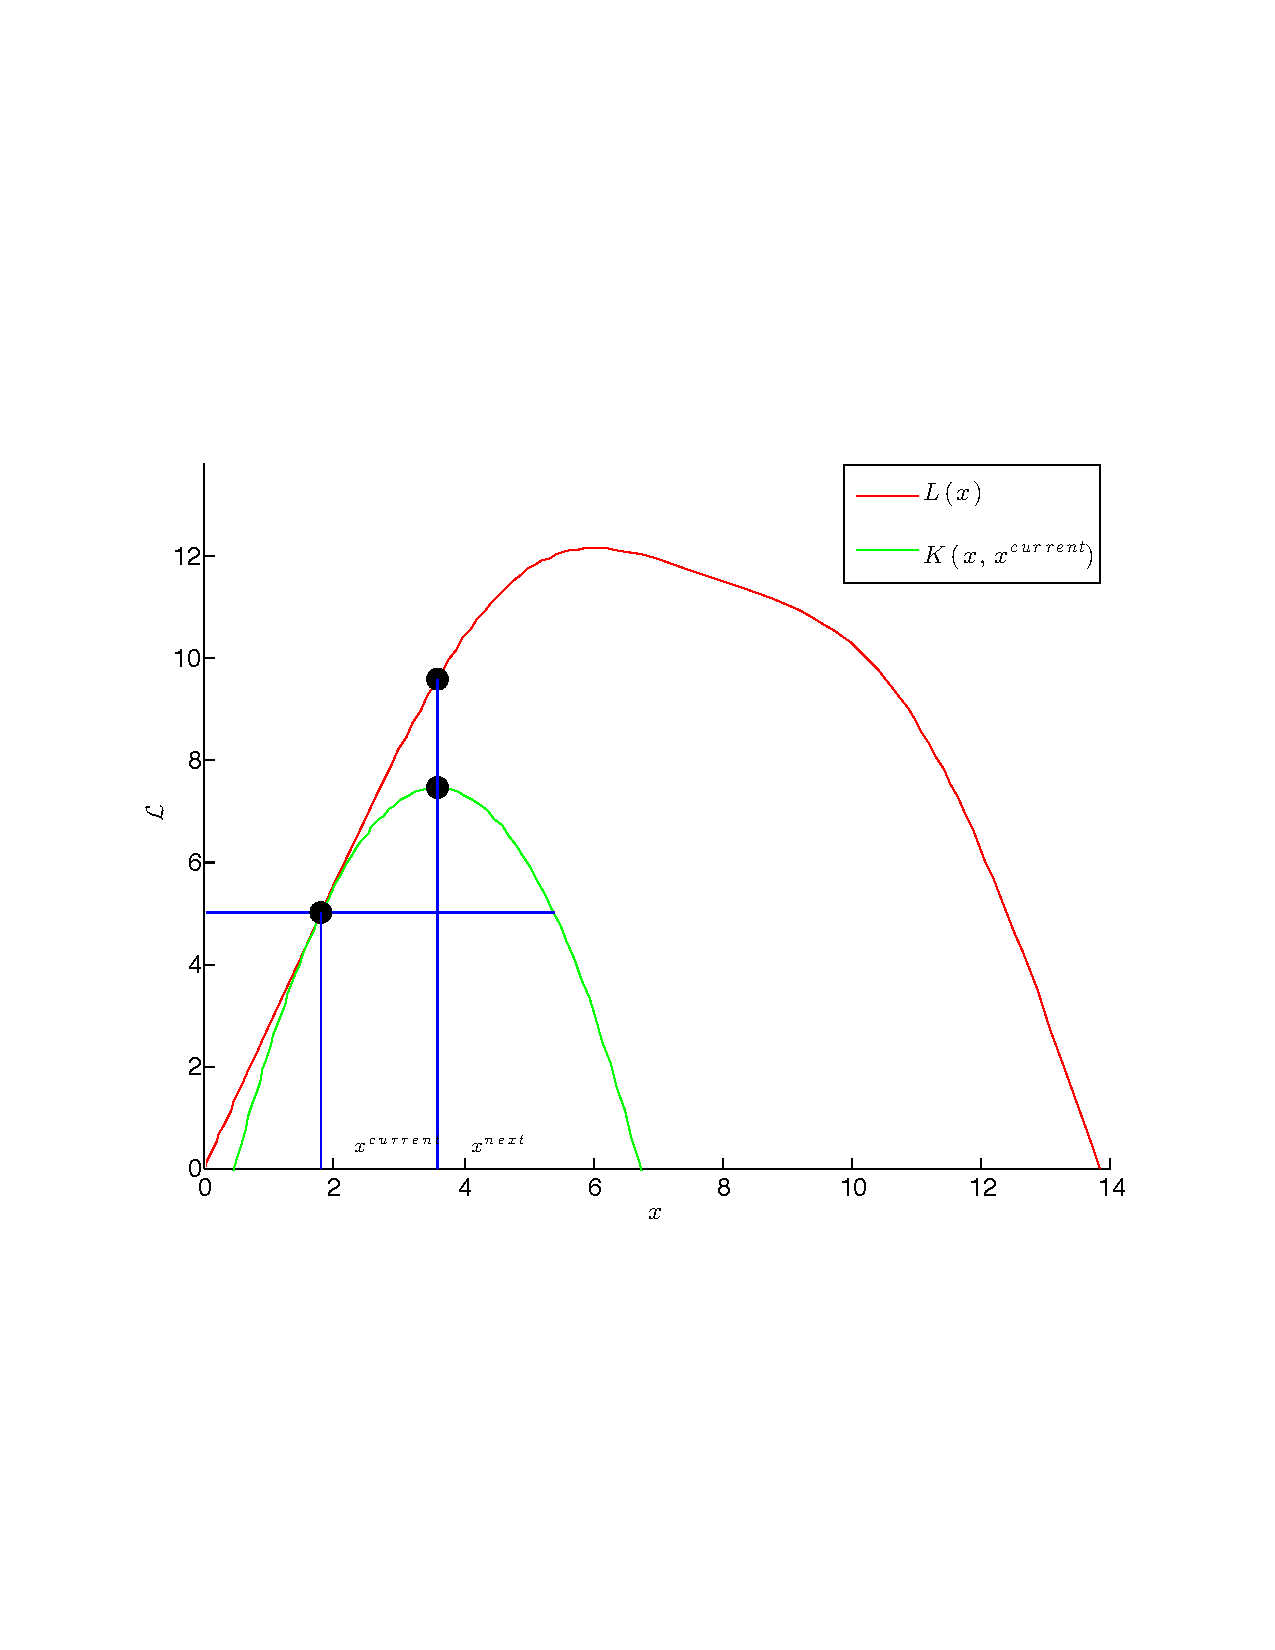
\includegraphics[width=\linewidth]{figures/isra}
  	\end{minipage}\hfill
  	\begin{minipage}[t]{0.4\textwidth}
    	\caption{\emph{An example of an iteration of the ISRA algorithm. The function to be optimised is $L(x)$. The surrogate function $K(x,x^{current})$ is easier to optimise and produces the next parameter estimation.}}
  	\end{minipage}
\end{figure}




%----------------------------------------------------------------------------
\subsubsection*{Derivation of ISRA}
If the data is assumed to have a normal distribution, and the system matrix is non-negative ($\forall i,j\ :\ a_{ij} \geq 0$), and the image is non-negative ($\forall j\ :\ x_j \geq 0$), and the variance is assumed to be independent of $i$ ($\forall \sigma_i\ :\ \sigma_i = \sigma$) , then the log-likelihood is
\begin{align}
	L(\vec x) = -\frac{1}{2 \sigma^2}\sum_i\left( -y_i + \sum_j a_{ij}x_j
	\right)^2
\end{align}

where terms that do not depend on $\vec x$ are neglected. The optimisation is not influenced by $\sigma$ therefore set $\sigma = 1$. If the null space of the system matrix is trivial, the function $L(\vec x)$ is strictly concave and it has a unique maximum.\\

The following expression can be used as surrogate function
\begin{align}
	K(\vec x, \vec b) = -\frac{1}{2} \sum_i\sum_j 
	\frac{a_{ij}b_j}{\sum_qa_{ij}b_q}
	\left( -y_i + \frac{x_j}{b_j} \sum_r a_{ir}b_r \right)^2
\end{align}

where $b_j > 0$ is the current estimate of the parameter $x_j$. Check now that this function satisfies the required conditions for the surrogate function as stated above.\\

The first condition on the surrogate function is $\forall \vec x, \vec b \in \mathbb{R}^n \ :\ K(\vec x, \vec b) \leq L(\vec x)$. Define
\begin{align}
	w_{ij} = \frac{a_{ij}b_j}{\sum_q a_{iq}b_q}
\end{align}

Remark that for a certain fixed data index $i$, the $w_{ij}$ are normalised positive weights: $w_{ij} \geq 0$ and $\sum_j w_{ij} = 1$. Here the non-negativity of the system matrix was used. Then
\begin{align}
	L(\vec x) - K(\vec x, \vec b) &= -\frac{1}{2}\sum_i 
	\left[\left( \sum_j w_{ij}z_{ij} \right)^2
	- \sum_j w_{ij}z_{ij}^2
	\right]
	\\
	%
	\shortintertext{with}
	z_{ij} &= -y_i + \frac{x_j}{b_j} \sum_k a_{ik}b_k
\end{align}


Cauchy-Schwarz's inequality states 
\begin{eqnarray}
	\left( \langle \vec u, \vec v \rangle \right)^2 \leq \left \| \vec u \right \|^2
	\left \| \vec v \right \|^2
\end{eqnarray}

Take
\begin{eqnarray}
	&&u_j = \sqrt{w_{ij}} z_{ij}\nonumber\\
	&&v_j = \sqrt{w_{ij}}\\
	\nonumber\\
	&&\Rightarrow \left \| \vec v \right \|^2 = 1
\end{eqnarray}

therefore
\begin{eqnarray}
	\left \| \vec u \right \|^2 = 
	\left( \sum w z^2 \right) \geq \left( \sum wz \right)^2
	\rightarrow L(\vec x) - K(\vec x, \vec b) \geq 0
\end{eqnarray}

This proves that condition 1 is met.\\

Condition 2 reads $\forall \vec b \in \mathbb{R}^n \ :\ K(\vec b, \vec b) = L(\vec b)$. This is clearly the case as can be seen from the expressions of $L$ and $K$.\\

The proposed surrogate function can be decomposed in the index $j = 1,\ ...\ ,n$ and optimised for each $j$. Doing so yields the ISRA iteration
\begin{align}
	\hat x_j^{next} = \hat x_j^{current}\frac
	{\sum_{i=1}^{m} a_{ij}y_i}
	{\sum_{p=1}^{m} \sum_{q=1}^{n} a_{pj}a_{pq}\hat x_q^{current}}\ \ \ \ \ j = 1,\ ...\ ,n
\end{align}

Conceptually this corresponds to an iteration of the form
\begin{align}
	\hat{\vec{x}}^{next} = \hat{\vec{x}}^{current} \frac{Backproject(\vec y)}{Backproject(\ Project(\hat{\vec{x}}^{current}))}
	\label{eq:ISRAConceptual}
\end{align}




%----------------------------------------------------------------------------
\subsection{OSEM}\label{sec:osem}
MLEM and ISRA are numerically stable algorithms that are guaranteed to converge, though convergence may need a large number of iterations and is computationally expensive. There exist algorithms such as OSEM that converge significantly faster but these algorithms are numerically less stable.\\

OSEM (Ordered Subset Expectation Maximisation) proposed by Hudson and Larkin \cite{OSEM}  is an adaptation of MLEM in which the data is partitioned in several distinct subsets. The number of subsets is defined as being the OS level and the data $\vec{y}$ is thus partitioned in subsets $\vec{s}$: $\vec{y} = \{\vec{s}_1, \vec{s}_2, ..., \vec{s}_{os}\}$. One iteration of OSEM then consists of applying MLEM on each subset $\vec{s}$. Remark that one iteration of OSEM takes about the same amount of time as one iteration of MLEM, and remark also that OSEM with just 1 subset containing all the data is simply MLEM.\\

It turns out that applying such an approach introduces an increase in convergence speed that is proportional to the OS level. If for example the data is divided in 32 subsets, then OSEM (level 32) can be expected to achieve a reconstruction quality at iteration 1 that is comparable to MLEM reconstruction quality at iteration 32. An example is shown in figure \ref{fig:OSEMThorax}. 

Though increasing the number of subsets does increase the convergence speed significantly there are limits as to the number of subsets than can be used on noisy data. Using more subsets increases noise due to artefacts in the case of noisy data. This can partially, but not completely, be avoided by stopping the algorithm early, before it converges.\\

Hudson and Larkin \cite{OSEM} gave a proof of convergence for OSEM assuming exact data and balanced subsets\footnote{Subsets are referred to as balanced if they are selected in such a way that the activity in a pixel contributes equally to each subset.}. In the case of noisy data, OSEM does not converge to a ML solution. Empirically it seems that OSEM converges to a cycle of limit images. It should be noted that with a modest number of subsets, these limit images are barely, if at all, distinguishable from each other and can be considered equal for all practical purposes. 

If a ML solution is needed, OSEM can be adapted to converge to a ML solution by decreasing the number of subsets gradually (e.g. 32 subsets for iteration 1, 16 for it 2, ..., 2 for it 5, and 1 subset for iteration 6 and up). This approach still speeds up the convergence, but converges to a ML solution in the end.\\

A final note on ordered subset is that this method of dividing the data in subsets in order to increase the speed of convergence is not limited to MLEM. Other reconstruction algorithms such as ISRA can employ the same ordered subset method as well by simply applying the corresponding algorithm on each subset. The results of applying the ordered subset method on other reconstruction algorithms are comparable to the MLEM case.
\begin{figure}[H]
	\centering
	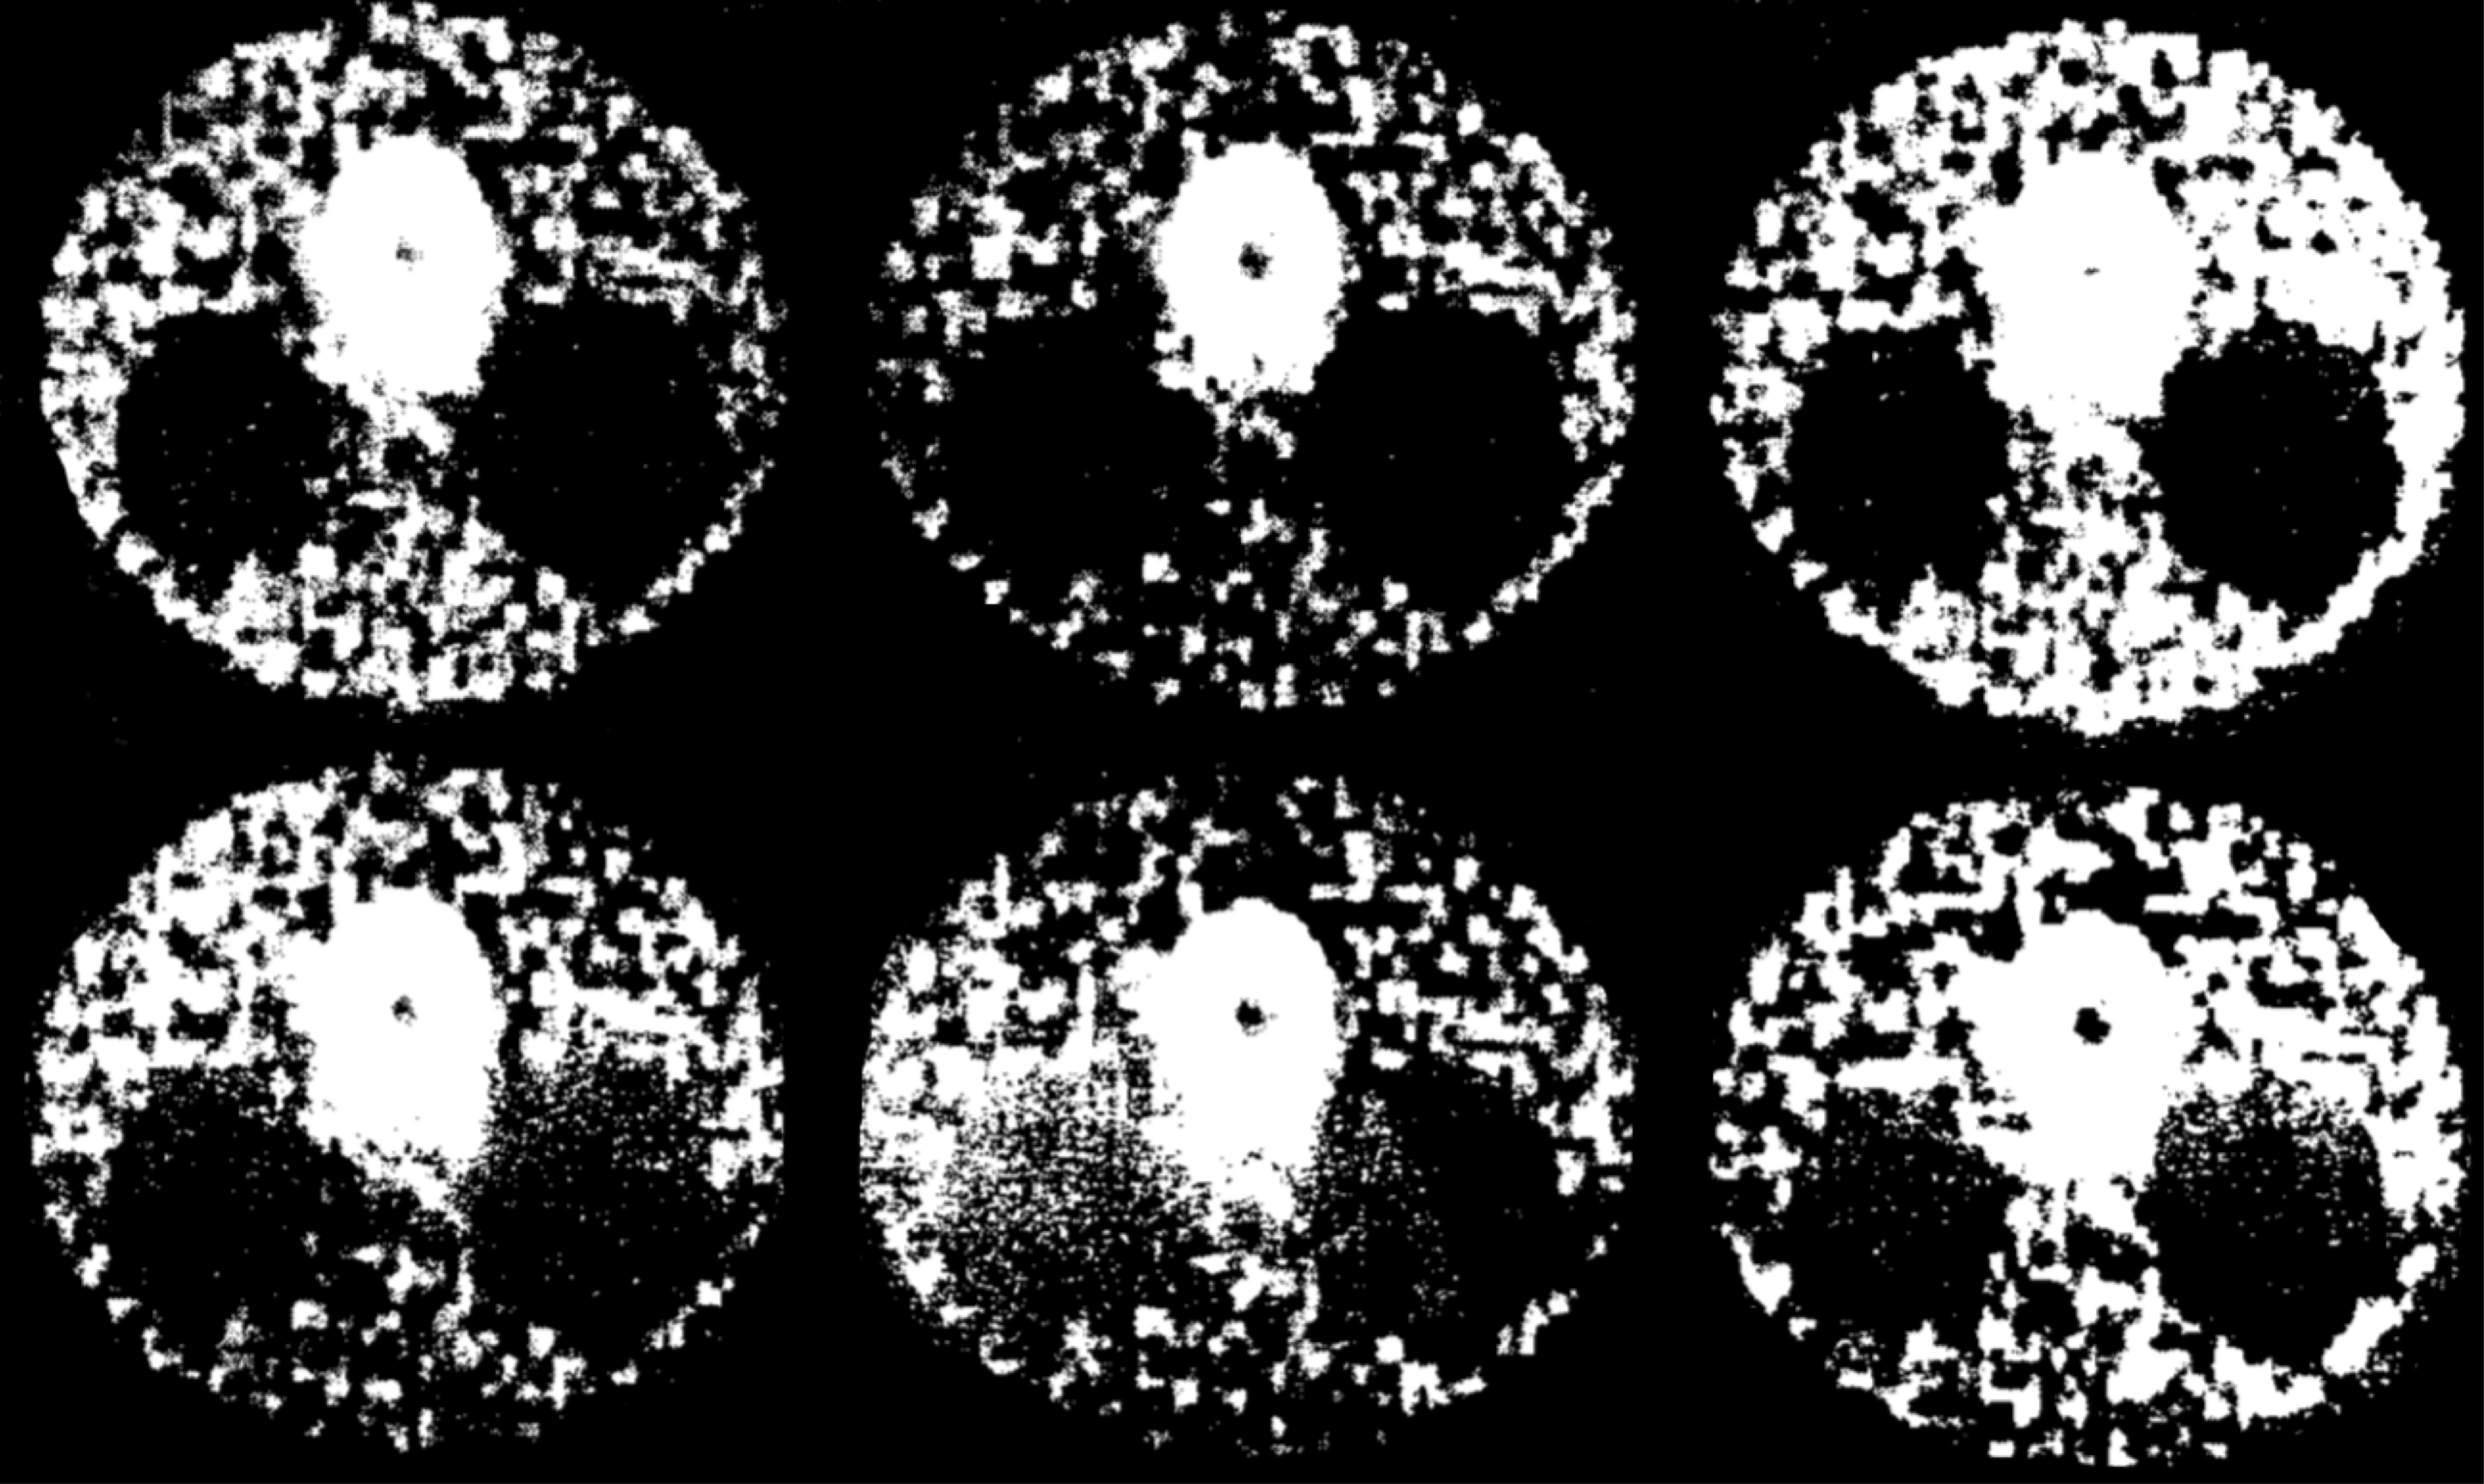
\includegraphics[width=.58\linewidth]{figures/OSEMThorax}
	\caption{\emph{OSEM introduces a gain in iteration speed that is proportional to the OS level. Reconstructed image of a thorax phantom after matched iterations. Remark that the images achieve comparable reconstruction qualities. Image reprinted from \cite{OSEM}.\\
	TOP: level 1: 32 iterations, level 2: 16 iterations, level 4: 8 iterations.\\
	BOTTOM: level 8: 4 iterations, level 16: 2 iterations, level 32: 1 iteration. }}
	\label{fig:OSEMThorax}
\end{figure}

\newpage




%----------------------------------------------------------------------------
%Study of a toy problem
%----------------------------------------------------------------------------
\chapter{Study of a toy problem}
This chapter presents a simple toy problem that can be estimated with PET image reconstruction methods. This will help develop a feeling for the mathematics and computational tools involved with PET. It will also allow to derive some closed form expressions that may be too complicated to derive for a real PET problem.\\

Imagine an image reconstruction problem where the image to be reconstructed is only 1 pixel high by 2 pixels wide. In each of these pixels, there can be some activity from a tracer. The decay particles emitted by the tracer can be detected by detectors placed around the image. For this problem, the detectors are only capable of collecting data along 3 specific LORs and measure de facto the line integral of the activity along the path. The problem is then to estimate the activity $x_j$ in each pixel, given some data $y_i$ from the detectors after collecting data for a certain time $t$. The setup is represented in detail in figure \ref{fig:toyproblem}.\\
\begin{figure}[h]
	\centering
	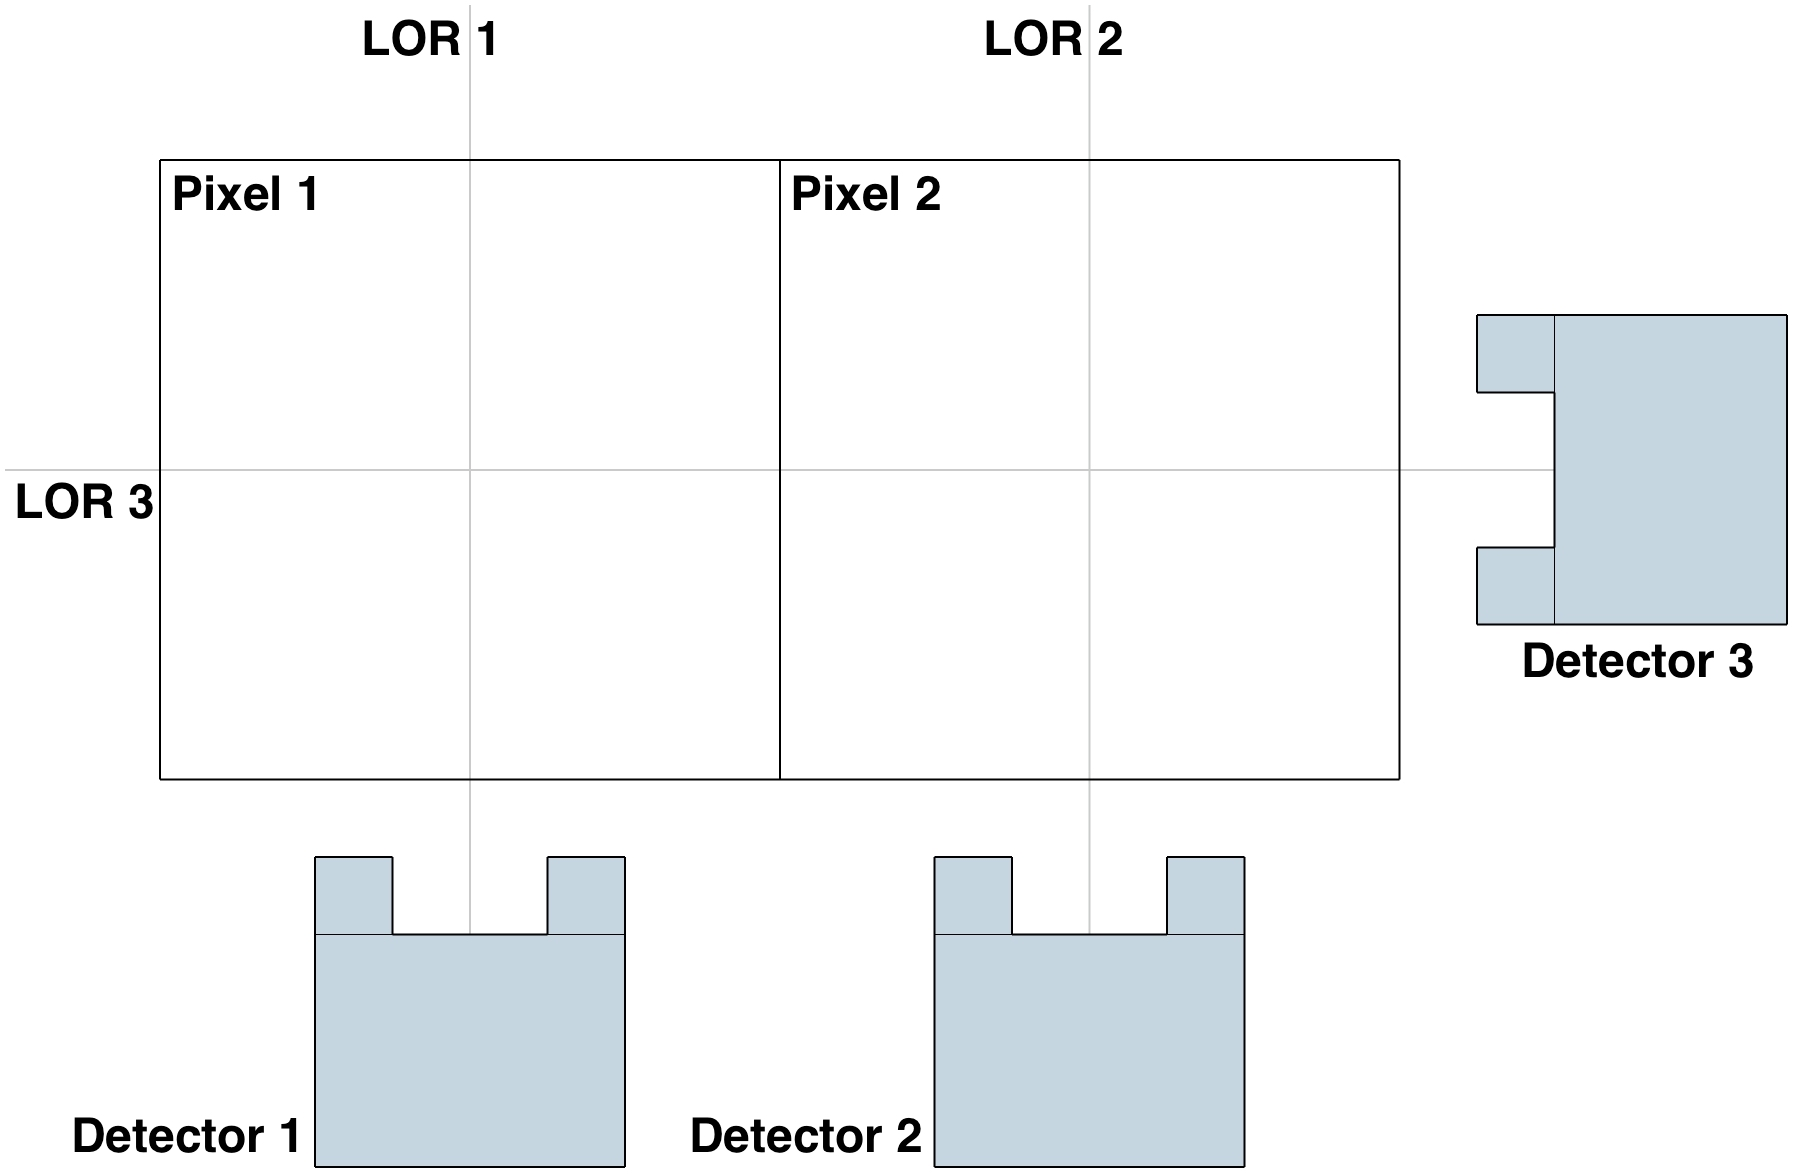
\includegraphics[width=0.55\textwidth]{figures/fig_toyProblem.jpg}
	\caption{\emph{A 2 pixel toy problem with 3 specific lines of response.}}
	\label{fig:toyproblem}
\end{figure}

Mathematically the problem can be expressed as a matrix multiplication
\begin{align}
	Y = AX
	\label{eq:toyproblemsetup}
\end{align}

where the column vector Y contains all the data $y_i$ with $i: 1 \rightarrow m$. The column vector X contains all the unknown values of the activities $x_j$  with $j: 1 \rightarrow n$ in the different pixels. A is referred to as the system matrix. It is an $m \times n$ matrix which links the $m$ detectors to the $n$ data sources. The system matrix must model the geometry of the setup to determine how much the activity in a given pixel contributes to the data acquisition of a certain detector. The system matrix can also model effects such as detector sensibility, attenuation, blurring and positron range \cite{china}. It should be no surprise that a system matrix that describes these effect more accurately produces a better reconstruction \cite{system matrix errors}.\\

In general expression \ref{eq:toyproblemsetup} has the form
\begin{align}
	\left[ \begin{array}{c} 
	y_{1} \\ y_{2} \\ \vdots \\ y_{m} 
	\end{array} \right]
	%
	= \left[ \begin{array}{cccc} 
	a_{11} & a_{12} & \cdots &a_{1n} \\ 
	a_{21} & a_{22} & \cdots &a_{2n} \\ 
	\vdots & \vdots & \ddots & \vdots\\
	a_{m1} & a_{m2} & \cdots &a_{mn} 
	\end{array} \right].
	%
	\left[ \begin{array}{c} 
	x_{1} \\ x_{2} \\ \cdots \\x_{n} 
	\end{array} \right]
\end{align}

where the $y_i$'s are the measurements from the $m$ detectors, the $x_j$'s are the activities in the $n$ pixels, and the $a_{ij}$'s are the system matrix elements where $a_{ij}$ is the contribution from the $j$\superscript{th} pixel to the $i$\superscript{th} detector.\\

For this specific problem, there are 3 detectors and 2 pixels. So the system matrix should be a 3 x 2 matrix. From the setup in fig. \ref{fig:toyproblem} it is should be obvious that the part of the system matrix that accounts for the geometry of the setup is
\begin{align}
	A = \left[ \begin{array}{cc} 1 & 0 \\ 0 & 1 \\ 1 & 1 \end{array} \right]
\end{align}

So the problem can be stated in matrix form as
\begin{align}
	\left[ \begin{array}{c} 
	y_1 \\ y_2 \\ y_3 
	\end{array} \right]  
	=
	\left[ \begin{array}{cc} 
	1 & 0 \\ 0 & 1 \\ 1 & 1 
	\end{array} \right]
	.
	\left[ \begin{array}{c} x_1 \\ x_2 \end{array} \right] 
	\label{eq:toyproblem}
\end{align}

Remark that on the left side of this equation are the dimensionless data measurements (in 'units of events detected'), while on the right side are the image parameters as activities with dimension $[T^{-1}]$. To solve the dimension problem and to account for the measurement time (which is a crucial parameter in PET), the system matrix needs to also incorporate the time. The  equation to be used becomes
\begin{align}
	\left[ \begin{array}{c} 
	y_1 \\ y_2 \\ y_3 
	\end{array} \right]  
	=
	\left[ \begin{array}{cc} 
	t & 0 \\ 0 & t \\ t & t 
	\end{array} \right]
	.
	\left[ \begin{array}{c} x_1 \\ x_2 \end{array} \right] 
	\label{eq:e}
\end{align}

the following sections will discuss various methods to estimate the activities $x_1$ and $x_2$ based on the data $y_1$, $y_2$ and $y_3$. The time parameter $t$ will be shown to be a crucial parameter: longer measurement times significantly improve the reconstruction quality.\\

Remark that for this simple problem the model and the system matrix only account for the geometry of the problem. Detector sensibility, attenuation, blurring and positron range are not accounted for.




%----------------------------------------------------------------------------
\section{Derivation of closed form expressions}
The maximum likelihood method to estimate parameters from a data set can be used to solve the toy problem. The ML method has been presented in section \ref{sec:mlmethod}. To actually estimate the true, unknown values of the image $x_j$ with ML estimators $\hat x_{j, (ml)}$, the setup and problem have to be studied and the likelihood must be modelled.\\

For this problem it is almost trivial to assume a Poisson data distribution because the emission process is Poisson, because the system matrix only considers geometrical effects and because dead-time is not considered. So for the toy problem ML estimators will be derived from a Poisson likelihood and their main properties will also be derived.\\

One of the goals of this thesis is to determine how assuming a Gaussian data distribution influences the reconstructed image's quality so the ML estimators and their properties will also be derived from a Gaussian likelihood.\\




%----------------------------------------------------------------------------
\subsection{Poisson maximum likelihood estimation}\label{sec:ML}
If the data $y_1$, $y_2$ and $y_3$ are assumed to be independent and Poisson distributed then the likelihood of obtaining the data set $\{y_1, y_2, y_3\}$, given the parameters $\{x_1, x_2\}$ is
\begin{align}
	\mathcal{L} \left( (y_1, y_2, y_3) \mid (x_1, x_2) \right) 
	&= 
	\prod_{i=1}^{3} e^{-\lambda_i} \frac{\lambda_i^{y_i}}{y_i!}
	\nonumber\\
	%
	&= \prod_{i=1}^{3} exp\left(-\sum_{j=1}^{2}a_{ij}x_j\right)
	\frac{(\sum_{j=1}^{2}a_{ij}x_j)^{y_i}}{y_i!}
	\label{eq:likelihoodtoy}
\end{align}

Working out first the sum and then the product in eq. \ref{eq:likelihoodtoy}, and using that the system matrix elements $a_{ij}$ are either t or 0, the likelihood is
\begin{align}
	\mathcal{L} 
	&= 
	\prod_{i=1}^{3} exp(-a_{i1}x_1 - a_{i2}x_2) 
	\frac{(a_{i1}x_1 + a_{i2}x_2)^{y_i}}{y_i!}
	\nonumber\\
	%
	&= e^{-t.x_1} \frac{(t.x_1)^{y_1}}{y_1!}\ .\  
	e^{-t.x_2} \frac{(t.x_2)^{y_2}}{y_2!}\ .\
	e^{-t.(x_1 + x_2)} \frac{t^{y_3}(x_1 + x_2)^{y_3}}{y_3!}
	\nonumber\\
	%
	&= \frac{t^{y_1 + y_2 + y_3} . 
	e^{-2t(x_1+x_2)}\ .\ x_1^{y_1}\ .\ x_2^{y_2}.(x_1+x_2)^{y_3}}
	{y_1!\ y_2!\ y_3!}
\end{align}

The log-likelihood is then
\begin{align}
	l &= ln\ \mathcal{L}
	\nonumber\\
	%
	&= ln\left( \frac{t^{y_1 + y_2 + y_3} . 
	e^{-2t(x_1+x_2)}\ .\ x_1^{y_1}\ .\ x_2^{y_2}.(x_1+x_2)^{y_3}}
	{y_1!\ y_2!\ y_3!} \right)
	\nonumber\\
	%
	&= ln\left( 
	t^{y_1 + y_2 + y_3} . 
	e^{-2t(x_1+x_2)}\ .\ x_1^{y_1}\ .\ x_2^{y_2}.(x_1+x_2)^{y_3} 
	\right) - 
	ln\left( y_1!\ y_2!\ y_3! \right)
	\nonumber\\
	%
	&= - 2t(x_1+x_2) + y_1\ ln(x_1) + y_2\ ln(x_2) + y_3\ ln(x_1+x_2) 
	\nonumber\\
	&\phantom{= }+ (y_1 + y_2 + y_3)\ ln(t) - ln\left( y_1!\ y_2!\ y_3! \right)
	\nonumber\\
	\label{eq:f}
\end{align}

To solve the problem, the unknown parameters $x_1$ and $x_2$ are to be estimated. To do so the scores must first be determined from the log-likelihood. These are simply the partial derivative of the log-likelihood to the parameters to be estimated
\begin{align}
	S_j((y_1, y_2, y_3) \mid (x_1, x_2)) 
	= \frac{\partial ln\ \mathcal{L} 
	\left( (y_1, y_2, y_3) \mid (x_1, x_2) \right)}{\partial x_j}
	= \frac{\partial l}{\partial x_j}
\end{align}

Then, with the log likelihood from eq. \ref{eq:f}, the scores become
\begin{align}
	S(x_1) &= -2t + \frac{y_1}{x_1} + \frac{y_3}{x_1 + x_2}
	\nonumber\\
	%
	S(x_2) &= -2t + \frac{y_2}{x_2} + \frac{y_3}{x_1+x_2}
	\label{eq:scoremltoy}
\end{align}

The ML estimators are finally found by maximising the likelihood. Since the scores are the derivatives of the log-likelihood to the parameters, the ML estimators for the parameters are found by setting all scores to zero and solving the system of equations
\begin{align}
	&\left\{\begin{array}{cc} 
	S( \hat x_{1, ml} ) 
	= -2t + \frac{ y_1}{ \hat x_{1, ml}} + 
	\frac{ y_3 }{\hat x_{1, ml} + \hat x_{2, ml}} = 0\\
	\\
	%
	S( \hat x_{2, ml} ) 
	= -2t + \frac{ y_2}{ \hat x_{2, ml}} + 
	\frac{ y_3 }{\hat x_{1, ml} + \hat x_{2, ml}} = 0\\
	\end{array}\right.
	\nonumber\\
	%
	&...
	\nonumber\\
	%
	\Rightarrow
	&\left\{\begin{array}{cc} 
	\hat x_{1, ml} = \frac{y_1(y_1 + y_2 + y_3)}{2t(y_1 + y_2)}\\ 
	\\
	%
	\hat x_{2, ml} = \frac{y_2(y_1 + y_2 + y_3)}{2t(y_1 + y_{2})}   
	\end{array}\right.
	\label{eq:toyMLGeneral}
\end{align}

So the ML estimators for the toy problem are given by eq. \ref{eq:toyMLGeneral}.\\

A subtlety is that the ML estimators from eq. \ref{eq:toyMLGeneral} were found assuming that $y_1 + y_2 \neq 0$. From the expressions of the ML estimators in eq. \ref{eq:toyMLGeneral} it is clear that if $y_1 + y_2 = 0$, the ML estimators break down. Because the measurements are a number of events, $y_1$ and $y_2$ can not be negative. The question then is what the correct ML estimators are if both $y_1$ and $y_2$ are zero. From the setup in figure \ref{fig:toyproblem} it is clear that if $y_1$ and $y_2$ are zero, it will be difficult to give statistical information about the individual parameters $x_1$ and $x_2$.\\

The scores with $y_1 = y_2 = 0$ can be read directly from eq. \ref{eq:scoremltoy}
\begin{align}
	S(x_1) &= -2t + 0 + \frac{y_3}{x_1+x_2}
	\nonumber\\
	%
	S(x_2) &= -2t + 0 + \frac{y_3}{x_1+x_2}
\end{align}

The ML estimators are once again found by setting the score equal to zero and solving for the parameters. Remark that the system of equations is underdetermined and there can be no hope of finding an unique solution. Lacking any more information and having no a priori reason to believe that one pixel contributes more than the other, it is reasonable to distribute the estimated activity equally over both pixels. So set $\hat x_{1, ml} = \hat x_{2, ml}$ and the special case ML estimators become
\begin{align}
	&- 2t + \frac{y_3}{\hat x_{1, ml} + \hat x_{2, ml}} = 0
	\nonumber\\
	%
	&\Rightarrow \hat x_{1, ml} = \hat x_{2, ml} = \frac{y_3}{4t}
\end{align}

The complete solution to the ML estimators is then
\begin{align}
	(y_1 + y_2) \neq 0\ : \
	&\left\{\begin{array}{cc} 
	\hat x_{1, ml} = \frac{y_1(y_1 + y_2 + y_3)}{2t(y_1 + y_2)}\\ 
	\nonumber\\
	%
	\hat x_{2, ml} = \frac{y_2(y_1 + y_2 + y_3)}{2t(y_1 + y_{2})}   
	\end{array}\right.
	\nonumber\\
	%
	(y_1 + y_2) = 0\ : \
	&\left\{\begin{array}{cc} 
	\hat x_{1, ml} = \frac{y_3}{4t}\\ 
	\nonumber\\
	%
	\hat x_{2, ml} = \frac{y_3}{4t}   
	\end{array}\right.
	\\
	\label{eq:toyMLComplete}
\end{align}

From eq. \ref{eq:toyMLComplete} it is clear that the estimators $\hat x_{1, ml}$ and $\hat x_{2, ml}$ are completely symmetrical under exchange of $j=1 \leftrightarrow 2$. Some of the important properties of $\hat x_{1,ml}$ will be discussed. The case $\hat x_{2,ml}$ is completely analogous.\\

An important property of an estimator is its variance. The derivation of the exact variance of the ML estimator is a tedious one. The exact result was found by Cloquet et al. \cite{MLEM and OSEM Deviate} and is given here without derivation
\begin{align}
	var(\hat x_{1,ml}) = &-\left\{ x_1 + (x_2 - x_1) \frac{e^{-t \mu}}{4} \right\} ^2\nonumber\\
			&+\frac{e^{-t \mu}}{16 t^2} \left\{ t \mu + (t \mu)^2 \right\}\nonumber\\
			&+\frac{t x_1 + t^2x_1^2}{4t^2}\nonumber\\
			&+\frac{1}{2t \mu} \left\{ \nu(1-e^{-t \mu}) + x_1^2 t \mu \right\}\nonumber\\
			&+\frac{1}{4} \left\{ \frac{t \mu + (t \mu)^2}{(t \mu)^2} \right\}\nonumber\\
			&\times \left\{ x_1^2 (1-e^{-t \mu}) + \nu G (t \mu) \right\}
	\label{eq:varML}
\end{align}

where $\mu = x_1 + x_2$, $\nu = x_1 x_2$ and $G(t\mu) = \sum_{s=1}^{\infty} s^{-1} e^{-t\mu} (t\mu)^{s} / s!$.\\

Another important property of an estimator is its expected value, and closely related its bias. Again the derivation of the expected value of the ML estimator $\hat x_{1, ml}$ is not straight forward, but Cloquet et al. \cite{MLEM and OSEM Deviate} managed to find a closed form expression for the expected value as well
\begin{align}
	E[\hat x_{1,ml}] = x_1 - \frac{e^{-t(x_1 + x_2)}}{4} 
	(x_1 - x_2)
	\label{eq:expectedValueML}
\end{align}

The bias is given by eq. \ref{eq:bias}
\begin{align}
	b(\hat x_j) &= E[\hat x_j] - x_{j}
\end{align}

So the ML estimator $\hat x_{1, ml}$ is biased and its bias is
\begin{align}
	b(\hat x_{1, ml}) 
	&=  x_1 - \frac{e^{-t(x_1 + x_2)}}{4} 
	(x_1 - x_2) - x_1
	\nonumber\\
	%
	&= \frac{-e^{-t(x_1 + x_2)}}{4} 
	(x_1 - x_2)
	\label{eq:biasML}
\end{align}

Due to the power $-t$ in the exponential, the estimator $\hat x_{1, ml}$ is asymptotically unbiased for large $t$.\\

A last quantity worth investigating is the CR bound. Because the computation of the CR bound does not depend on the estimator itself (at least for the unbiased case), but only on the (presumed) distribution of the data, it is a universal lower bound. The derivation of the CR bound as given here assumes that the data has a Poisson distribution. Relevant for the ML estimator is it is both unbiased and efficient for large samples. Unfortunately for PET the samples are limited in size and the CR bound is not reached.\\

There are multiple (2) parameters so the matrix form of the CR bound should be used, which states that, assuming no bias, the variance of the $j$\superscript{th} parameter is equal to, or larger than the $j$\superscript{th} diagonal element of the inverse Fisher information matrix
\begin{align}
	var(\hat x_j) 
	\geq [I]^{-1}_{jj}
\end{align}

the Fisher information matrix is
\begin{align}
	[I(\vec x)]_{jj'}
	= -E\left[  
	\frac{\partial^2}{\partial x_j \partial x_{j'}} 
	ln\ \mathcal{L}(\vec y \mid \vec x)
	\right]
	= -E\left[  
	\frac{\partial^2}{\partial x_j \partial x_{j'}} 
	l
	\right]
\end{align}

which for the toy problem is
\begin{align}
	I(\vec x)
	&= -E\left[ \begin{array}{cc} 
	\frac{\partial^2}{\partial x_1 \partial x_1} l
	&
	\frac{\partial^2}{\partial x_1 \partial x_2} l
	\\
	\\
	\frac{\partial^2}{\partial x_2 \partial x_1} l
	&
	\frac{\partial^2}{\partial x_2 \partial x_2} l
	\end{array} \right]
	\nonumber\\
	\nonumber\\
	%
	&= -E \left[ \begin{array}{cc} 
	-\frac{y_1}{x_1^2} - \frac{y_3}{(x_1 + x_2)^2}
	&
	-\frac{y_3}{(x_1+x_2)^2}
	\\
	\\
	-\frac{y_3}{(x_1+x_2)^2}
	&
	-\frac{y_2}{x_2^2} - \frac{y_3}{(x_1 + x_2)^2}
	\end{array} \right]
	\label{eq:fishermatrixtoy}
\end{align}

where the log-likelihood of Poisson data was used. Because the expected value of a sum is the sum of the expected values, and because the expected values of $y_1, y_2$ and $y_3$ can be trivially derived from eq. \ref{eq:e} and the toy problem setup, the Fisher information matrix and its inverse are
\begin{align}
	[I(\vec x)]_{jj'}
	&= \left[ \begin{array}{cc} 
	\frac{t}{x_1} + \frac{t}{(x_1 + x_2)}
	&
	\frac{t}{(x_1+x_2)}
	\\
	\\
	\frac{t}{(x_1+x_2)}
	&
	\frac{t}{x_2} + \frac{t}{(x_1 + x_2)}
	\end{array} \right]
	\nonumber\\
	%
	[I(\vec x)]_{jj'}^{-1}
	&=
	\frac{1}{2t(x_1 + x_2)}
	\left[ \begin{array}{cc} 
	x_1^2 + 2 x_1 x_2
	&
	-x_1 x_2
	\\
	\\
	-x_1 x_2
	&
	x_2^2 + 2 x_1 x_2
	\end{array} \right]
	\label{eq:fisherInverseInformationMatrixToyML}
\end{align}

So for any unbiased estimators of $x_1$ the CR bound is
\begin{align}
	var(\hat x_1) &\geq \frac{x_1^2 + 2 x_1 x_2}{2t(x_1 + x_2)}
	\label{eq:crunbiased}
\end{align}

Unfortunately the ML estimators are biased and the matrix form of the biased CR bound as in eq. \ref{eq:CramerRaoMultiDim} must be used to determine a lower bound for the ML estimators.\\ 

Determine the Jacobian matrix
\begin{align}
	\left[ \frac{\partial E[\hat{\vec x}]}{\partial \vec x} \right] &= 
	\left[ \begin{array}{cc} 
	\frac{\partial E[\hat x_1]}{\partial x_1}
	&
	\frac{\partial E[\hat x_1]}{\partial x_2}
	\\
	\\
	\frac{\partial E[\hat x_2]}{\partial x_1}
	&
	\frac{\partial E[\hat x_2]}{\partial x_2}
	\end{array} \right]
	\nonumber\\
	%
	&= 
	\left[ \begin{array}{cc}
	1 + \big(t(x_1-x_2)-1\big)\frac{e^{-t(x_1+x_2)}}{4}\ \ \ \
	&
	\big(t(x_1-x_2)+1\big)\frac{e^{-t(x_1+x_2)}}{4}
	\\
	\\
	\big(t(x_2-x_1)+1\big)\frac{e^{-t(x_2+x_1)}}{4}\ \ \ \
	&
	1 + \big(t(x_2-x_1)-1\big)\frac{e^{-t(x_2+x_1)}}{4}
	\end{array} \right]
\end{align}

The Jacobian matrix's transpose is easily found and the inverse Fisher information matrix is given by \ref{eq:fisherInverseInformationMatrixToyML}. These three matrices allow determining the multidimensional biased CR bound which determines the lower bound on the covariance matrix of the parameters $x_1$ and $x_2$. Define
\begin{align}
	K \equiv \frac{e^{-t(x_2+x_1)}}{4}\ \ \ \ \
	L \equiv \frac{1}{2t(x_1 + x_2)}
\end{align}

Then
\begin{align}
	cov(\hat{\vec x}) \geq& \left[ \frac{\partial E[\hat{\vec x}]}{\partial \vec x} \right]\ \ .\ \ \Bigg[I(\vec x)\Bigg]^{-1} .\ \ \left[ \frac{\partial E[\hat{\vec x}]}{\partial \vec x} \right]^T
	\nonumber\\ 	\nonumber\\
	=\ &
	%
	\left[ \begin{array}{cc}
	1 + \big(t(x_1-x_2)-1\big)K\ \ \ \
	&
	\big(t(x_1-x_2)+1\big)K
	\\
	\\
	\big(t(x_2-x_1)+1\big)K\ \ \ \
	&
	1 + \big(t(x_2-x_1)-1\big)K
	\end{array} \right] .
	\nonumber\\ 	\nonumber\\
	%
	&L . 
	\left[ \begin{array}{cc} 
	x_1^2 + 2 x_1 x_2
	&
	-x_1 x_2
	\\
	\\
	-x_1 x_2
	&
	x_2^2 + 2 x_1 x_2
	\end{array} \right] .
	\nonumber\\ 	\nonumber\\
	%
	&\left[ \begin{array}{cc}
	1 + \big(t(x_1-x_2)-1\big)K\ \ \ \
	&
	\big(t(x_2-x_1)+1\big)K
	\\
	\\
	\big(t(x_1-x_2)+1\big)K\ \ \ \
	&
	1 + \big(t(x_2-x_1)-1\big)K
	\end{array} \right]
	\label{eq:label600}
\end{align}

This looks quite nasty and will (probably) not work out to a nice solution so if an explicit result is needed for the CR bound, the best course of action is to first evaluate all of the matrices' elements before doing the multiplication. 

Remark also that if $t$ and/or $x_1 + x_2$ becomes very large then K goes to 0, the diagonal elements of eq. \ref{eq:label600} reduce to the unbiased CR bounds for their respective estimators and the off-diagonal elements are 0.




%----------------------------------------------------------------------------
\subsection{Gaussian maximum likelihood estimation}\label{sec:LS}
The results from section \ref{sec:ML} were derived under the assumption that the data has a Poisson distribution. In practice this is (often) the case, but if the Poisson assumption does not hold because for example the data has been pre-corrected, or the detector dead-time is accounted for, an approximation can be made by assuming a Gaussian distribution for the data. To improve readability, to avoid confusion with the previous section, and because for Gaussian data a ML method produces the same estimators as an LS method the results derived in this section through a ML method will be labeled 'LS'. So the question is what the LS estimators for $x_1$ and $x_2$ and their variances are, assuming a normal distribution for the data collected by the detectors.\\

The data is assumed to have a normal distribution with a probability mass function of the form
\begin{align}
	P(y_i \mid \mu_i, \sigma_i^2) = \frac{1}{\sqrt{2 \pi \sigma_i^2}} 
	e^{\frac{-(y_i-\mu_i)^2}{2 \sigma_i^2}}
\end{align}

where the parameter $\mu_i$ is the expected value of $y_i$ and $\sigma_i^2$ the variance of $y_i$. Suppose that the variances of the data $\sigma_i^2$ are constant $\sigma^2$. Then
\begin{align}
	P(y_i \mid \mu_i, \sigma^2) = \frac{1}{\sqrt{2 \pi \sigma ^2}} 
	e^{\frac{-(y_i-\mu_i)^2}{2 \sigma^2}}
\end{align}

The expected value is
\begin{align}
	\mu_i = E[y_i] = \sum_{j=1}^{2}a_{ij}x_j
\end{align}

where the system matrix has the same form as before. If $y_1, y_2$ and $y_3$ are assumed to be independent the likelihood is
\begin{align}
	\mathcal{L} \left( (y_1, y_2, y_3) \mid (x_1, x_2) \right) 
	&= \prod_{i=1}^{3} \frac{1}{\sqrt{2 \pi \sigma^2}} 
	e^{\frac{-(y_i-\mu_i)^2}{2 \sigma^2}}
	\nonumber\\
	%
	&=(2\pi  \sigma^2)^{-\frac{3}{2}}
	e^{\frac{-1}{2 \sigma^2} \left( 
	(y_1 - \mu_1)^2 + (y_2 - \mu_2)^2 + (y_3 - \mu_3)^2 
	\right)}
\end{align}

Knowing the system matrix A, the expected values $\vec \mu$ are found to be $\mu_1 = t x_1$, $\mu_2 = t x_2$ and $\mu_3 = t(x_1 + x_2)$. The likelihood becomes
\begin{align}
	\mathcal{L} = 
	(2\pi \sigma^2)^{-\frac{3}{2}}
	e^{\frac{-1}{2 \sigma^2} \left( 
	(y_1 - t x_1)^2 + (y_2 - t x_2)^2 + (y_3 - t(x_1 + x_2))^2 
	\right)}
\end{align}

From the likelihood it is straight forward to determine the log-likelihood
\begin{align}
	l = - \frac{3}{2}\ ln(2\pi \sigma^2)
	-\frac{1}{2 \sigma^2} \left( 
	(y_1 - t x_1)^2 + (y_2 - t x_2)^2 + (y_3 - t(x_1 + x_2))^2 
	\right)
	%&= -\frac{3}{2} ln (2\pi) - \frac{1}{2}\left(
	%(y_1 - x_1)^2 + (y_2 - x_2)^2 + (y_3 - x_1 - x_2)^2) \right)
\end{align}

and from the log-likelihood, the scores become
\begin{align}
	&S((y_1, y_2, y_3) \mid x_j) = 
	\frac{\partial ln\ \mathcal{L} 
	\left( (y_1, y_2, y_3) \mid (x_1, x_2) \right)}{\partial x_j}
	= \frac{\partial l}{\partial x_j}
	\nonumber\\
	%
	&\Rightarrow S(x_1) 
	= \frac{t}{\sigma^2}\left( y_1 + y_3 - t x_2 - 2 t x_1 \right)
	\nonumber\\
	%
	&\Rightarrow S(x_2) 
	= \frac{t}{\sigma^2}\left( y_2 + y_3 - t x_1 - 2 t x_2 \right)
\end{align}

As per the usual method, the LS estimators can be found by setting the score to zero and solving the system of equations
\begin{align}
	&\left\{
	\begin{array}{cc} 
	S(\hat x_{1, ls}) = \frac{t}{\sigma^2}
	\left( y_1 + y_3 - t \hat x_{2, ls } - 2 t \hat x_{1, ls} \right)  
	\\
	\\
	S(\hat x_{2, ls }) = \frac{t}{\sigma^2}
	\left( y_2 + y_3 - t \hat x_{1, ls} - 2 t \hat x_{2, ls } \right)  
	\end{array}
	\right.
	\nonumber\\
	%
	&...
	\nonumber\\
	%
	\Rightarrow
	&\left\{
	\begin{array}{cc} 
	\hat x_{1, ls} = \frac{(2 y_1 - y_2 + y_3)}{3t}
	\\
	\\
	\hat x_{2, ls } = \frac{(2 y_2 - y_1 + y_3)}{3t}
	\end{array}
	\right.
	\label{eq:lsestiators}
\end{align}

It has been proven that an unconstrained LS estimator is unbiased for a linear problem. This is also true for $\hat x_{1, ls}$
\begin{align}
	E[\hat x_{1, ls}] 
	&= E\left[ \frac{2 y_1 - y_2 + y_3}{3t} \right]
	= \frac{1}{3t}\left( 2 E[y_1] - E[y_2] + E[y_3] \right)
	\nonumber\\
	%
	&=\frac{1}{3t} \left( 2 t x_1 - t x_2 + t(x_1 + x_2) \right)
	\nonumber\\
	%
	&= x_1
	\label{eq:biasnormalestimator}
\end{align}

and similar for the estimator $\hat x_{2, ls }$. As expected, these LS estimators are unbiased.\\

Having an unbiased estimator is a good thing, but what about the variance of these estimators? The variance of the LS estimator $\hat x_{1, ls}$ is found as a function of the variance of the data $\sigma^2$, and the measurement time $t$
\begin{align}
	var(\hat x_{1, ls}) 
	&= var\left(\frac{(2 y_1 - y_2 + y_3)}{3t}\right)
	= \frac{1}{9t^2}var\left(
	2y_1 - y_2 + y_3\right)
	\nonumber\\
	%
	&= \frac{1}{9t^2}\left(
	4\ var(y_1) + var(y_2) + var(y_3)\right)
	\nonumber\\
	%	
	&= \frac{1}{9t^2}\left(
	4 \sigma^2 + \sigma^2 + \sigma^2\right)
	\nonumber\\
	%
	&= \frac{6 \sigma^2}{9t^2} = \frac{2 \sigma^2}{3 t^2}
	\label{eq:varLS}
\end{align}

The above gives an exact result for the variance of the LS estimator $\hat x_{1, ls}$, but it still is interesting to see what the best possible variance is, which is given by the Cramer-Rao lower bound. To determine the Rao-Cramer bound, the Fisher information matrix must be computed first
\begin{align}
	&F(\vec x)
	= -E\left[ \begin{array}{cc} 
		\frac{\partial^2}{\partial x_1 \partial x_1} l
		&
		\frac{\partial^2}{\partial x_1 \partial x_2} l
		\\
		\\
		\frac{\partial^2}{\partial x_2 \partial x_1} l
		&
		\frac{\partial^2}{\partial x_2 \partial x_2} l
	\end{array} \right]
	%
	= -E \left[ \begin{array}{cc} 
		-\frac{2t^2}{\sigma^2}
		&
		-\frac{t^2}{\sigma^2}
		\\
		\\
		-\frac{t^2}{\sigma^2}
		&
		-\frac{2t^2}{\sigma^2}
		\end{array} \right]
		%
		= \frac{t^2}{\sigma^2}\left[ \begin{array}{cc} 
		2 & 1\\
		1 & 2
	\end{array} \right]
	\nonumber\\
	\nonumber\\
	%
	&\Rightarrow [F(\vec x)]^{-1} 
	= \frac{\sigma^2}{3t^2} 
	\left[\begin{array}{cc}
		2 & -1\\
		-1 & 2
	\end{array}\right]
\end{align}

So the CR lower bound for the variance of any unbiased estimator $\hat x_1$, where the data is assumed to have a normal distribution, is given by
\begin{align}
	var(\hat x_1) \geq \frac{2 \sigma^2}{3t^2}
	\label{eq:crnormal}
\end{align}

A reasonable assumption for the Gaussian distribution is that the data variance $\sigma^2$ is proportional to the measurement time $t$. In that case the CR bound for $var(\hat x_{1})$ is proportional to $t^{-1}$ just as for the true Poisson case eq. \ref{eq:crunbiased}.

Comparing eq. \ref{eq:varLS} and eq. \ref{eq:crnormal} shows that the LS estimator $\hat x_{1,ls}$ actually reaches the CR lower bound. It can be proven that any LS estimator for a linear problem reaches the CR bound. So for normally distributed data, the ML estimator and the LS estimator are the same, and they are always unbiased and efficient.\\

Remark that the CR bound given by \ref{eq:crnormal} only holds if the data are truly normal (which they are not). The LS estimators derived from approximating the likelihood with a Gaussian distribution are unbiassed, but they can not be expected to reach the CR bound based on the Poisson distribution.\\
 
The previous results show that it is possible to derive LS estimators if the Poisson assumption does not hold. These LS estimators were shown to be unbiased and efficient, if the assumption on the data distribution holds (which is not the case).




%----------------------------------------------------------------------------
\section{Reconstruction using simulated data}
In the previous sections, different estimators and iterative algorithms were derived to estimate the activity in each pixel of the toy problem. This section will examine computationally if the derived theoretical results are compatible with experimentally observed results by generating simulated data, and by computing and comparing the corresponding theoretical and experimental results.

\subsection{Maximum likelihood and least squares estimators}
It is possible to test the theoretical results derived in section \ref{sec:ML} for the ML estimators and in section \ref{sec:LS} for the LS estimators by simulating the problem.\\

The simulation is based on the generation of Poisson distributed data. It takes as input the activity in pixel 1: $x_1$, the activity in pixel 2: $x_2$, the measurement time: $t$, and a sample size parameter: $k$. The Poisson random data variables $y_1$, $y_2$ and $y_3$ with parameters $x_1$ and $x_2$ are simulated $k$ times with different noise realisations.
% \hfill\phantom{1}
%\setlength\intextsep{0pt}
%\begin{wrapfigure}{r}{0.4\textwidth}
%	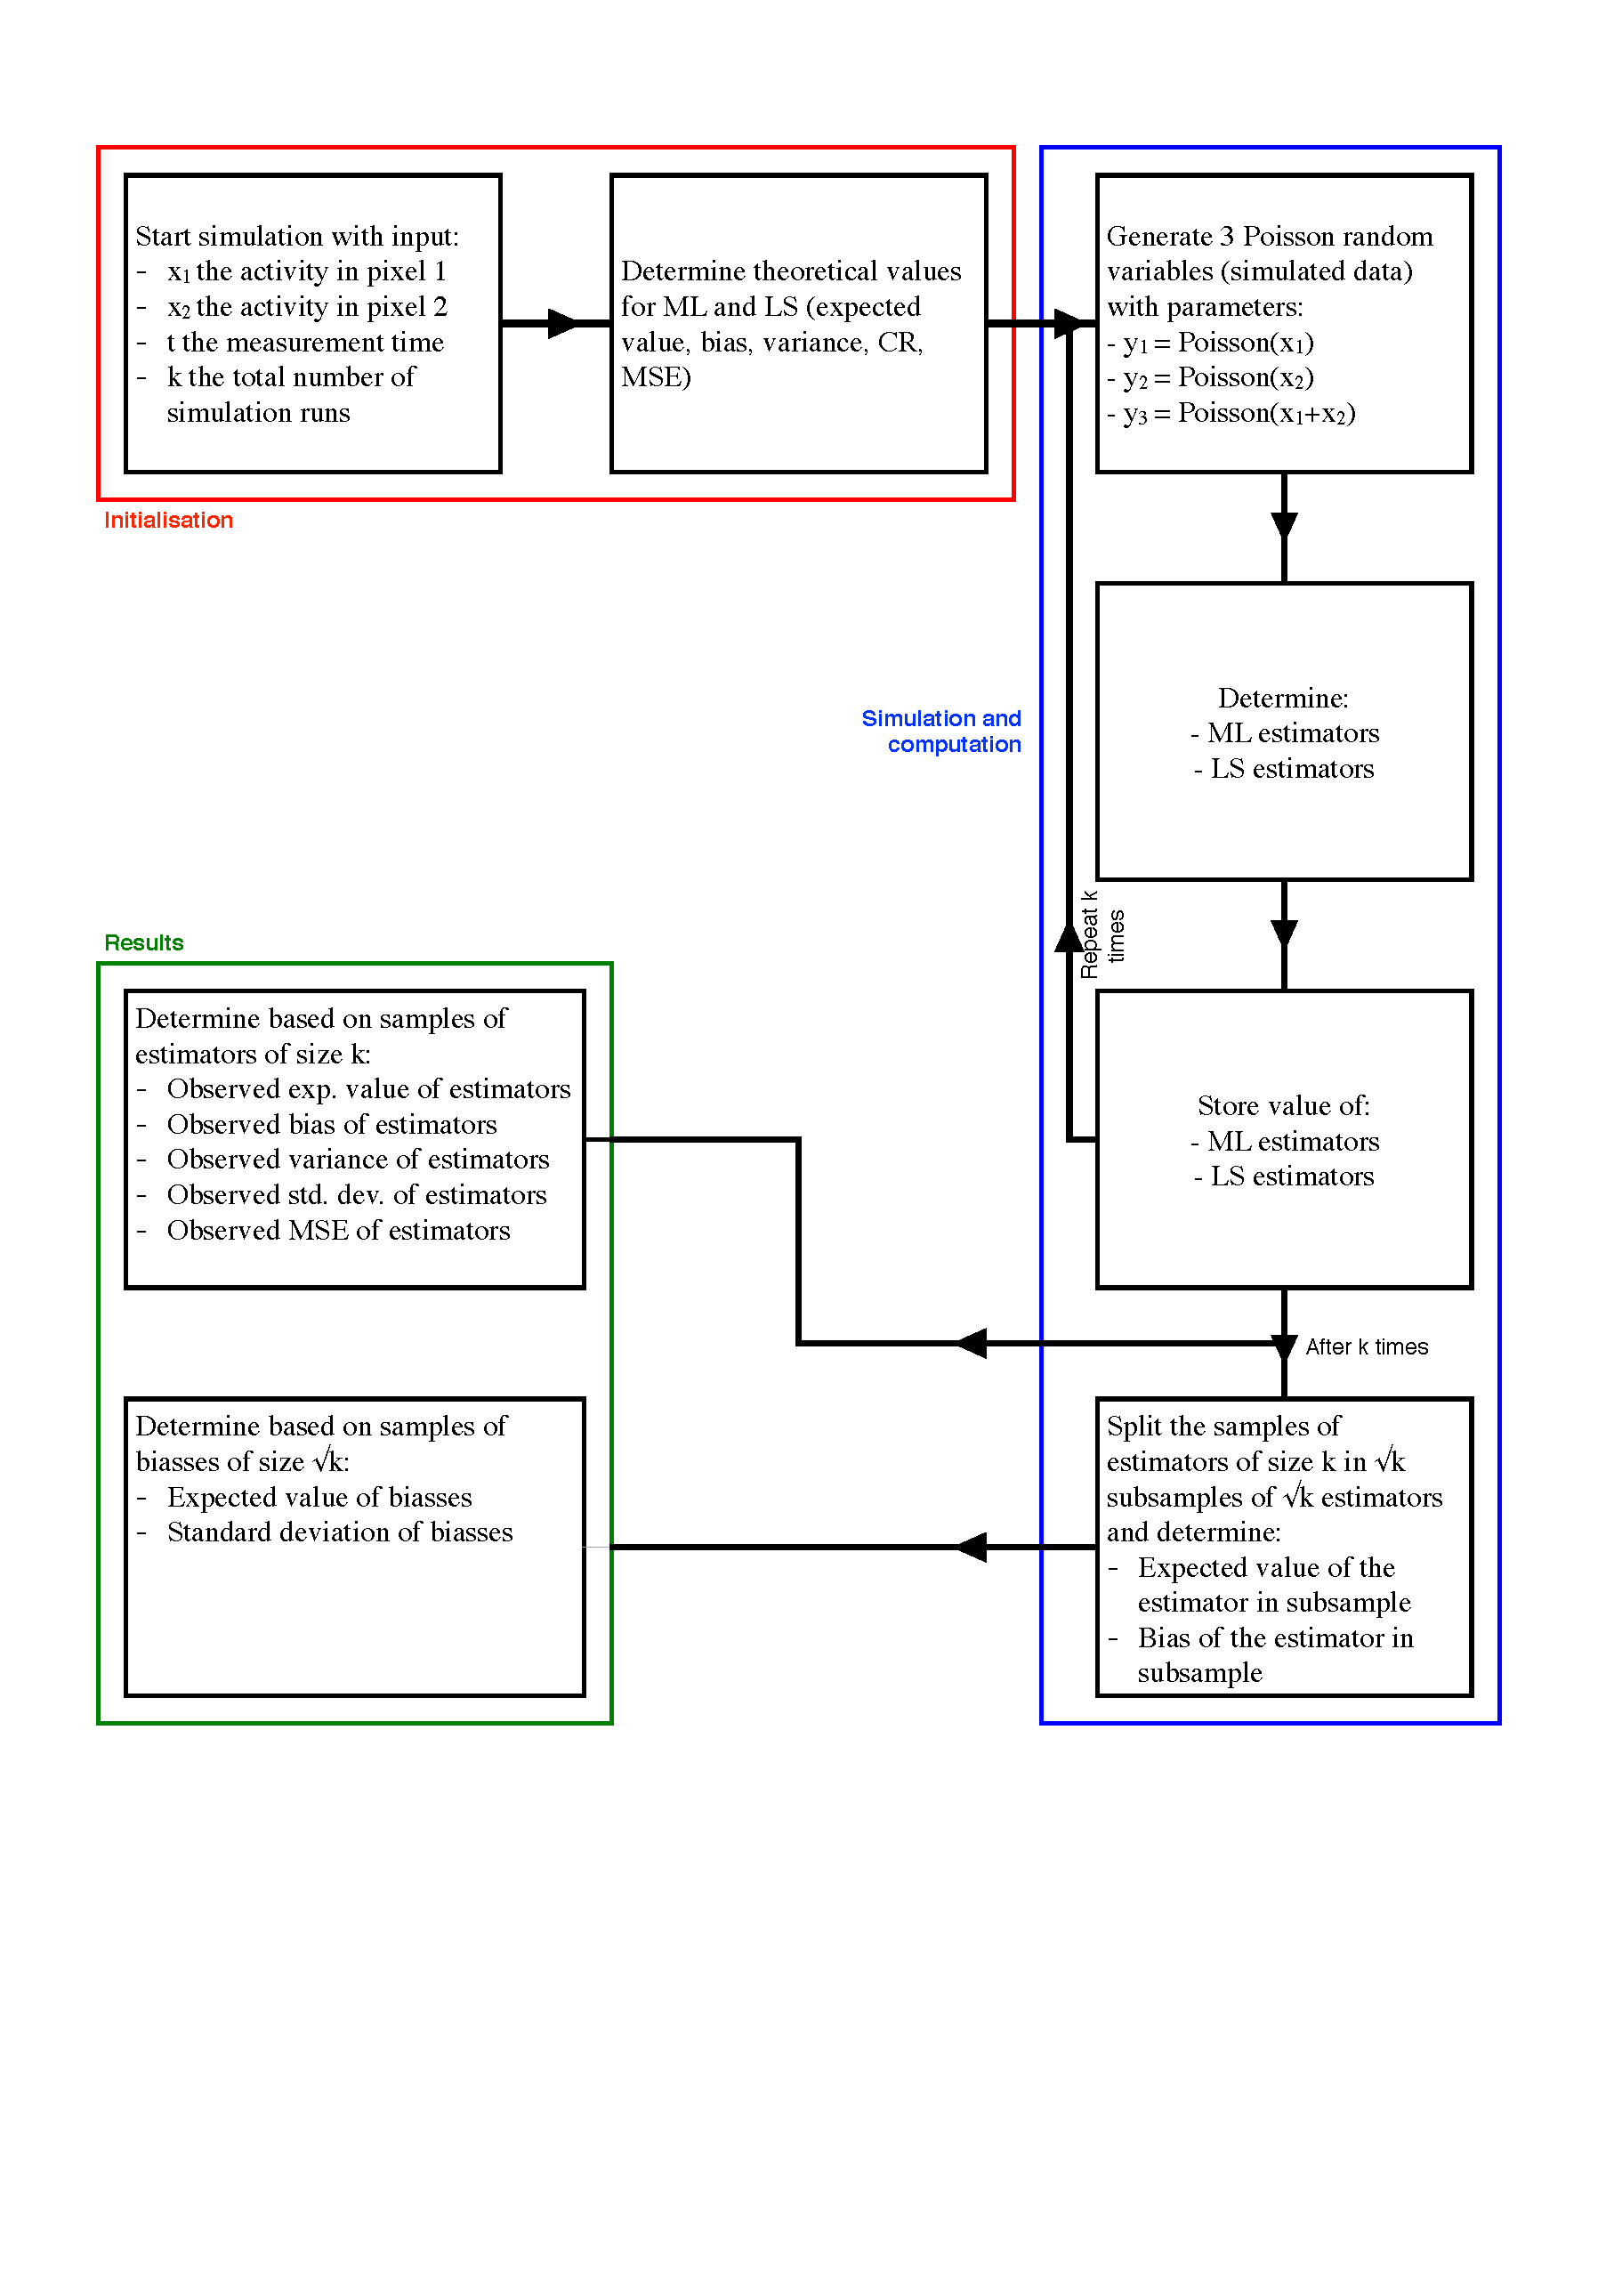
\includegraphics[width=0.4\textwidth]{figures/Simulation}
%	\caption{\emph{Flow chart of the simulation of the toy problem.}}
%	\label{fig:Simulation1}
%\end{wrapfigure}
%\intextsep\skip32\\

Based on these parameters and a Matlab build-in Poisson random variable generator, the data is simulated. With the true parameter values and the simulated data, it is possible to compute different theoretical and observed quantities. The most important quantities relevant to PET are the estimators' values, their expected values, their variances and their biasses. These quantities' theoretical and observed values are computed and compared. Additionally the CR bounds are determined to see how well the variances perform and the MSEs (Mean Square Error) are also determined to be able to compare the quality of the ML and LS estimators. The observed results are based on a sample of $k$ data simulations. The last quantity to be determined is an estimation of the error on the bias. The flowchart in figure \ref{fig:flowchartSimulation} gives a schematic overview of how the simulation is performed.\\
\begin{figure}[H]
	\centering
	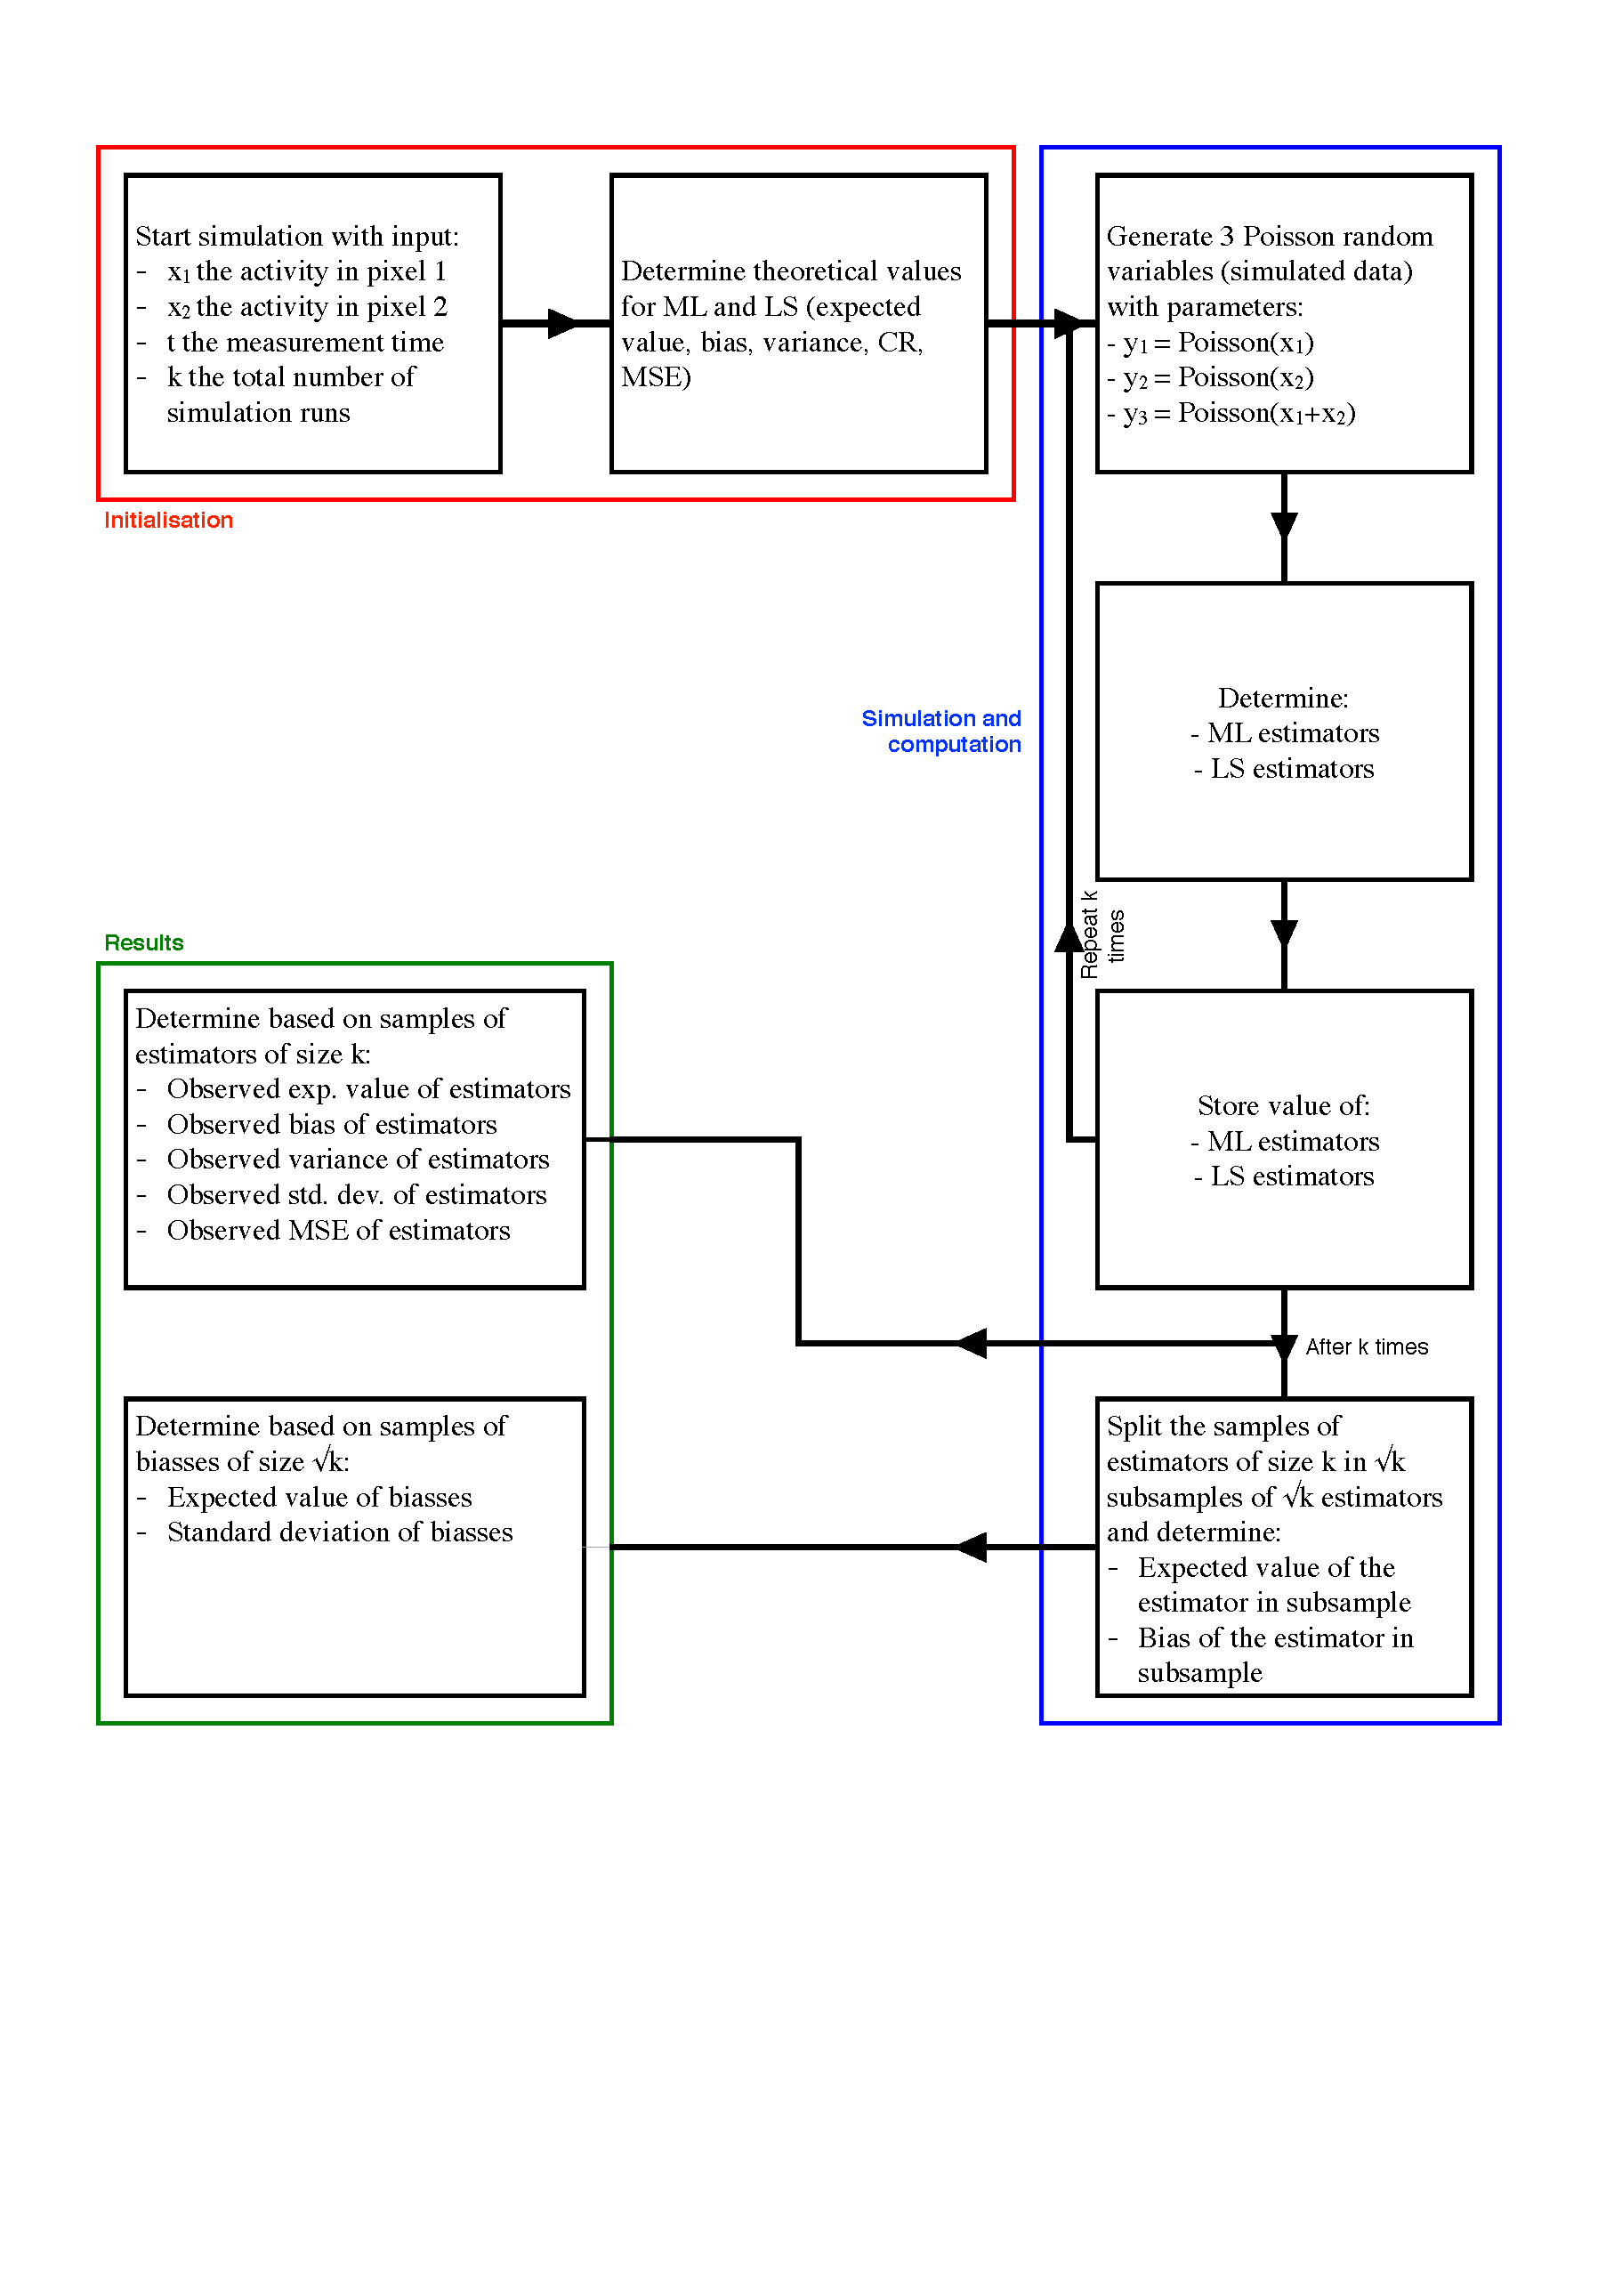
\includegraphics[width=.8\linewidth]{figures/Simulation.pdf}
	\caption{The flowchart for the simulation of the toy problem}
	\label{fig:flowchartSimulation}
\end{figure}

All the theoretical results were already derived in the previous sections. The ML estimators are given by eq. \ref{eq:toyMLComplete}. Their variances by eq. \ref{eq:varML}, their expected values by eq. \ref{eq:expectedValueML} and their biasses by eq. \ref{eq:biasML}. In the expression for the variance the factor $G(t\mu) = \sum_{s=1}^{\infty} s^{-1} e^{-t\mu} (t\mu)^{s} / s!$ might be  problematic. Notice that the factors $s^{-1}$ and $s!$ assure that the sum converges rapidly. Different methods such as brute forcing by computing all terms that the computer can handle or using Stirling's approximation can be used to determine or at least approximate this sum. In this case Wolfram|Alpha was used to find a results for $G(t\mu)$ whenever it was encountered. The CR bounds for the ML estimators can be found by solving eq. \ref{eq:label600}.\\

The ML estimators are based on the assumption that the data is Poisson. One of the goals is to determine what happens if an LS estimator based on a Gaussian data distribution is used instead of a 'true' Poisson ML estimator. The estimators to use are the LS estimators given by eq. \ref{eq:lsestiators}. Their expected values are trivially given by eq. \ref{eq:biasnormalestimator} and their variances can be found by starting from eq. \ref{eq:varLS}
\begin{align}
	var(\hat x_{1, ls})
	&= \frac{1}{9t^2}\left(
	4\ var(y_1) + var(y_2) + var(y_3)\right)
\end{align}

The data $y_1$, $y_2$ and $y_3$ are Poisson with respective parameters $\lambda_1$, $\lambda_2$ and $\lambda_3$. It has been proven in the first chapter that the variance of a Poisson distribution is the parameter of that distribution. So the variances of the LS estimators becomes
\begin{align}
	var(\hat x_{1, ls}) &= \frac{1}{9 t^2} \left( 4 \lambda_1 + \lambda_2 + \lambda_3 \right)
	\nonumber\\
	%
	&= \frac{1}{9 t^2} \left( 
	4 x_{1}t + x_{2}t + 
	(x_{1} + x_{2})t 
	\right)
	\\
	%
	var(\hat x_{2, ls }) &= \frac{1}{9 t^2} \left( 
	4 x_{2}t + x_{1}t + 
	(x_{1} + x_{2})t 
	\right)
\end{align}

where is should be clear from the setup in figure \ref{fig:toyproblem} why the parameters $\lambda_1$, $\lambda_2$ and $\lambda_3$ are equal to respectively $x_1$, $x_2$ and $x_1 + x_2$.\\

It has been proven that for an LS estimator the CR bound is reached and that the bias is zero. But in this case, the LS estimators are an approximation assuming a Gaussian data distribution, while the 'true' CR bound is derived from the model's Poisson distribution. The CR bound to be used is the unbiased eq. \ref{eq:crunbiased}. It is not expected to be reached because the Gaussian assumption does not hold.\\

It is possible to determine the observed values of the different estimators based on the simulated data. The observed expected values of the estimators can be computed with the law of large numbers as the average of all computed estimators (assuming the simulated data set is large enough)
\begin{align}
	obs\ E[\hat x] = \frac{1}{k} \sum_{i=1}^{k} \left(\hat x_i \right)
\end{align}

and their variances and standard deviations
\begin{align}
	obs\ var(\hat x) &= \frac{1}{k-1} \sum_{i=1}^{k}
	\big(\hat x_i - E[\hat x]\big)
	\\
	%
	obs\ \sigma(\hat x) &= \sqrt{obs\ var(\hat x)}
	\label{eq:variance}
\end{align}

Because the true values of the estimators are known in this simulation (the true values are the parameters of the simulation), it is easy to determine the biasses on the estimators
\begin{align}	
	obs\ b(\hat x) &= obs\ E[\hat x] - x
	\nonumber\\
	%
	&= \widehat{E[\hat x - x]}
\end{align}

With the variances and biasses of the estimators it is straight-forward to determine the MSE
\begin{align}
	MSE(\hat x) = var(\hat x) + \left(b(\hat x)\right)^2
\end{align}

The MSE enables to compare the quality of estimators with possibly a different bias. The best possible estimator is an estimator that has 0 variance and 0 bias, so the closer the MSE of an estimator gets to 0, the better the estimator is considered to be.\\

Two additional quantities are computed to determine whether the biasses are inherent of the estimators or just statistical fluctuations. The data is simulated $k$ times, producing a sample of $k$ estimators. Based on this sample the expected values, biasses and variances of the estimators are computed. To determine whether the bias of any estimator is inherent to the estimator or just a statistical fluctuation, an expected value and variance can be associated to each numerical estimation of the bias.

The sample consists of $k$ estimators of $x = x_1$ or $x_2$. Split this sample in $\sqrt{k}$ samples of $\sqrt{k}$ estimators. Based on each of these samples of $\sqrt{k}$ estimators, determine the expected value $E[\hat x]_{_{\sqrt{k}}} = (1/\sqrt(k))\sum_{i=1}^{\sqrt{k}} \hat x_i$ of the estimator and then its bias $b(\hat x)_{_{\sqrt{k}}} = E[\hat x]_{_{\sqrt{k}}} - x$. This results in a set of $\sqrt{k}$ numerical estimations of the bias. The expected value, variance and standard deviation of this set can be determined and may help decide whether the bias is inherent of the estimator. The expected value of the set of numerical estimators of the bias is noted as
\begin{align}
E[\{b_{_{\sqrt{k}}}(\hat x)\}] = \frac{1}{\sqrt{k}} \sum_{i=1}^{\sqrt{k}} \big( b_{i_{\sqrt{k}}}(\hat x) \big)
\end{align}

and the standard deviation of this set is
\begin{align}
\sigma(\{b_{_{\sqrt{k}}}(\hat x)\}) = \sqrt{\frac{1}{\sqrt{k}-1}\sum_{i=1}^{\sqrt{k}}\big( b_{i_{\sqrt{k}}} - E[\{b_{_{\sqrt{k}}}(\hat x)\}]\big)}
\end{align}

Two simulations were performed: one with small parameter values and therefore sparse data counts and a second with larger parameter values and therefore more data counts. The different results are in table \ref{tab:simulation1} and table \ref{tab:simulation2}. Several conclusions can be drawn from these results:
\begin{itemize}
	\item All theoretical values correspond almost exactly with the observed values. This shows that the numerical results are compatible with the theory.
	
	\item The ML estimators are biased for small parameter values, but not for larger values, confirming that ML estimators are asymptotically unbiased.
	
	\item The LS estimators are as expected unbiased.
		
	\item The MSE's of the ML estimators are in general a bit smaller that the MSE's of the LS estimators, but the difference is not significant enough to claim that the ML estimators are better than the LS estimators for this problem.

	\item With large parameter values and many data counts, the CR bound is the same for the ML and LS estimators, which is to be expected because the ML estimators are asymptotically unbiased.
		
	\item With large parameter values and high data counts, both the ML and LS estimators nearly reach the CR bound.
\end{itemize}

In figure \ref{fig:biasToyProblem} top and figure \ref{fig:biasToyProblem}  bottom the effect of the time on the bias of the ML, respectively LS estimators is investigated. The observed bias is plotted as a function of the time and the error on the bias is estimated by $\sigma(\{b_{_{\sqrt{k}}}(\hat x)\})$. Because both ML and LS estimators were already shown to be (asymptotically) unbiased only the case with small parameter values is considered. From those plots it can be concluded that 
\begin{itemize}
	\item The ML estimators are asymptotically unbiased.
	
	\item The LS estimators are always unbiased.
	
	\item The estimation of the error on the numerical estimator of the bias decreases slowly in the beginning and quickly stabilises.
\end{itemize}









\begin{table}[H]
\centering
\centerline{
\begin{tabular}{lrrlrrlrrlrr}
\cline{2-12}
\multicolumn{1}{l|}{}                                                & \multicolumn{11}{l|}{Simulation of the toy problem with parameters:}                                                                                                                                                                                                                                                            \\
\multicolumn{1}{l|}{}                                                & \multicolumn{2}{l}{$x_1 = 0.1$}                            &                       & \multicolumn{2}{l}{$x_2 = 1.0$}                               &                       & \multicolumn{2}{l}{$t = 1$}                                 &                       & \multicolumn{2}{l|}{$k = 1\ 000\ 000$}                      \\ \cline{2-12} 
                                                                     & \multicolumn{1}{l}{}         & \multicolumn{1}{l}{}         &                       & \multicolumn{1}{l}{}          & \multicolumn{1}{l}{}          &                       & \multicolumn{1}{l}{}         & \multicolumn{1}{l}{}         &                       & \multicolumn{1}{l}{}         & \multicolumn{1}{l}{}         \\ \cline{2-3} \cline{5-6} \cline{8-9} \cline{11-12} 
\multicolumn{1}{l|}{}                                                & \multicolumn{2}{c|}{$\hat x_{1, ml}$}                       & \multicolumn{1}{c|}{} & \multicolumn{2}{c|}{$\hat x_{2, ml}$}                         & \multicolumn{1}{c|}{} & \multicolumn{2}{c|}{$\hat x_{1, ls}$}                       & \multicolumn{1}{c|}{} & \multicolumn{2}{c|}{$\hat x_{2, ls}$}                       \\ \cline{2-3} \cline{5-6} \cline{8-9} \cline{11-12} 
\multicolumn{1}{l|}{}                                                & \multicolumn{1}{c|}{Theo.}   & \multicolumn{1}{c|}{Obs.}    & \multicolumn{1}{c|}{} & \multicolumn{1}{c|}{Theo.}    & \multicolumn{1}{c|}{Obs.}     & \multicolumn{1}{c|}{} & \multicolumn{1}{c|}{Theo.}   & \multicolumn{1}{c|}{Obs.}    & \multicolumn{1}{c|}{} & \multicolumn{1}{c|}{Theo.}   & \multicolumn{1}{c|}{Obs.}    \\ \cline{1-3} \cline{5-6} \cline{8-9} \cline{11-12} 
\multicolumn{1}{|l|}{$E[\hat x]$}                                    & \multicolumn{1}{r|}{0.17490} & \multicolumn{1}{r|}{0.17481} & \multicolumn{1}{l|}{} & \multicolumn{1}{r|}{0.92510}  & \multicolumn{1}{r|}{0.92538}  & \multicolumn{1}{l|}{} & \multicolumn{1}{r|}{0.10000} & \multicolumn{1}{r|}{0.10022} & \multicolumn{1}{l|}{} & \multicolumn{1}{r|}{1.00000} & \multicolumn{1}{r|}{1.00019} \\
\multicolumn{1}{|l|}{$b(\hat x)$}                                    & \multicolumn{1}{r|}{0.07490} & \multicolumn{1}{r|}{0.07481} & \multicolumn{1}{l|}{} & \multicolumn{1}{r|}{-0.07490} & \multicolumn{1}{r|}{-0.07462} & \multicolumn{1}{l|}{} & \multicolumn{1}{r|}{0.00000} & \multicolumn{1}{r|}{0.00022} & \multicolumn{1}{l|}{} & \multicolumn{1}{r|}{0.00000} & \multicolumn{1}{r|}{0.00019} \\
\multicolumn{1}{|l|}{$\sigma(\hat x)$}                               & \multicolumn{1}{r|}{0.32746} & \multicolumn{1}{r|}{0.32680} & \multicolumn{1}{l|}{} & \multicolumn{1}{r|}{0.75148}  & \multicolumn{1}{r|}{0.75176}  & \multicolumn{1}{l|}{} & \multicolumn{1}{r|}{0.52705} & \multicolumn{1}{r|}{0.52657} & \multicolumn{1}{l|}{} & \multicolumn{1}{r|}{0.76020} & \multicolumn{1}{r|}{0.76013} \\
\multicolumn{1}{|l|}{$var(\hat x)$}                                  & \multicolumn{1}{r|}{0.10723} & \multicolumn{1}{r|}{0.10680} & \multicolumn{1}{l|}{} & \multicolumn{1}{r|}{0.56472}  & \multicolumn{1}{r|}{0.56514}  & \multicolumn{1}{l|}{} & \multicolumn{1}{r|}{0.27778} & \multicolumn{1}{r|}{0.27727} & \multicolumn{1}{l|}{} & \multicolumn{1}{r|}{0.57778} & \multicolumn{1}{r|}{0.57780} \\ \cline{1-3} \cline{5-6} \cline{8-9} \cline{11-12} 
\multicolumn{1}{|l|}{$CR$}                                           & \multicolumn{1}{r|}{0.06706} & \multicolumn{1}{r|}{-}       & \multicolumn{1}{l|}{} & \multicolumn{1}{r|}{0.52455}  & \multicolumn{1}{r|}{-}        & \multicolumn{1}{l|}{} & \multicolumn{1}{r|}{0.09545} & \multicolumn{1}{r|}{-}       & \multicolumn{1}{l|}{} & \multicolumn{1}{r|}{0.54545} & \multicolumn{1}{r|}{-}       \\ \cline{1-3} \cline{5-6} \cline{8-9} \cline{11-12} 
\multicolumn{1}{|l|}{$E\big [\{b_{_{\sqrt{k}}}(\hat x)\}\big ]$}     & \multicolumn{1}{r|}{-}       & \multicolumn{1}{r|}{0.07481} & \multicolumn{1}{l|}{} & \multicolumn{1}{r|}{-}        & \multicolumn{1}{r|}{-0.07462} & \multicolumn{1}{l|}{} & \multicolumn{1}{r|}{-}       & \multicolumn{1}{r|}{0.00022} & \multicolumn{1}{l|}{} & \multicolumn{1}{r|}{-}       & \multicolumn{1}{r|}{0.00019} \\
\multicolumn{1}{|l|}{$\sigma \big(\{b_{_{\sqrt{k}}}(\hat x)\}\big)$} & \multicolumn{1}{r|}{-}       & \multicolumn{1}{r|}{0.01049} & \multicolumn{1}{l|}{} & \multicolumn{1}{r|}{-}        & \multicolumn{1}{r|}{0.02418}  & \multicolumn{1}{l|}{} & \multicolumn{1}{r|}{-}       & \multicolumn{1}{r|}{0.01706} & \multicolumn{1}{l|}{} & \multicolumn{1}{r|}{-}       & \multicolumn{1}{r|}{0.02422} \\ \cline{1-3} \cline{5-6} \cline{8-9} \cline{11-12} 
\multicolumn{1}{|l|}{$MSE$}                                          & \multicolumn{1}{r|}{0.11284} & \multicolumn{1}{r|}{0.11240} & \multicolumn{1}{l|}{} & \multicolumn{1}{r|}{0.57033}  & \multicolumn{1}{r|}{0.57071}  & \multicolumn{1}{l|}{} & \multicolumn{1}{r|}{0.27778} & \multicolumn{1}{r|}{0.27727} & \multicolumn{1}{l|}{} & \multicolumn{1}{r|}{0.57778} & \multicolumn{1}{r|}{0.57780} \\ \cline{1-3} \cline{5-6} \cline{8-9} \cline{11-12} 
\end{tabular}}
\caption{\emph{The toy problem is simulated with small values for the activities and measurement time. The theoretical values are very close to the observed values which confirms the theoretical predictions.}}
\label{tab:simulation1}

\hfill\\
\hfill\\
\hfill\\
\hfill\\

\centerline{
\begin{tabular}{lrrlrrlrrlrr}
\cline{2-12}
\multicolumn{1}{l|}{}                                                & \multicolumn{11}{l|}{Simulation of the toy problem with parameters:}                                                                                                                                                                                                                                                               \\
\multicolumn{1}{l|}{}                                                & \multicolumn{2}{l}{$x_1 = 5$}                              &                       & \multicolumn{2}{l}{$x_2 = 10$}                                &                       & \multicolumn{2}{l}{$t = 10$}                                 &                       & \multicolumn{2}{l|}{$k = 1\ 000\ 000$}                        \\ \cline{2-12} 
                                                                     & \multicolumn{1}{l}{}         & \multicolumn{1}{l}{}         &                       & \multicolumn{1}{l}{}          & \multicolumn{1}{l}{}          &                       & \multicolumn{1}{l}{}         & \multicolumn{1}{l}{}          &                       & \multicolumn{1}{l}{}          & \multicolumn{1}{l}{}          \\ \cline{2-3} \cline{5-6} \cline{8-9} \cline{11-12} 
\multicolumn{1}{l|}{}                                                & \multicolumn{2}{c|}{$\hat x_{1, ml}$}                       & \multicolumn{1}{c|}{} & \multicolumn{2}{c|}{$\hat x_{2, ml}$}                         & \multicolumn{1}{c|}{} & \multicolumn{2}{c|}{$\hat x_{1, ls}$}                        & \multicolumn{1}{c|}{} & \multicolumn{2}{c|}{$\hat x_{2, ls}$}                         \\ \cline{2-3} \cline{5-6} \cline{8-9} \cline{11-12} 
\multicolumn{1}{l|}{}                                                & \multicolumn{1}{c|}{Theo.}   & \multicolumn{1}{c|}{Obs.}    & \multicolumn{1}{c|}{} & \multicolumn{1}{c|}{Theo.}    & \multicolumn{1}{c|}{Obs.}     & \multicolumn{1}{c|}{} & \multicolumn{1}{c|}{Theo.}   & \multicolumn{1}{c|}{Obs.}     & \multicolumn{1}{c|}{} & \multicolumn{1}{c|}{Theo.}    & \multicolumn{1}{c|}{Obs.}     \\ \cline{1-3} \cline{5-6} \cline{8-9} \cline{11-12} 
\multicolumn{1}{|l|}{$E[\hat x]$}                                    & \multicolumn{1}{r|}{5.00000} & \multicolumn{1}{r|}{5.00002} & \multicolumn{1}{l|}{} & \multicolumn{1}{r|}{10.00000} & \multicolumn{1}{r|}{9.99929}  & \multicolumn{1}{l|}{} & \multicolumn{1}{r|}{5.00000} & \multicolumn{1}{r|}{4.99972}  & \multicolumn{1}{l|}{} & \multicolumn{1}{r|}{10.00000} & \multicolumn{1}{r|}{9.99933}  \\
\multicolumn{1}{|l|}{$b(\hat x)$}                                    & \multicolumn{1}{r|}{0.00000} & \multicolumn{1}{r|}{0.00002} & \multicolumn{1}{l|}{} & \multicolumn{1}{r|}{0.00000}  & \multicolumn{1}{r|}{-0.00071} & \multicolumn{1}{l|}{} & \multicolumn{1}{r|}{0.00000} & \multicolumn{1}{r|}{-0.00028} & \multicolumn{1}{l|}{} & \multicolumn{1}{r|}{0.00000}  & \multicolumn{1}{r|}{-0.00067} \\
\multicolumn{1}{|l|}{$\sigma(\hat x)$}                               & \multicolumn{1}{r|}{0.64652} & \multicolumn{1}{r|}{0.64652} & \multicolumn{1}{l|}{} & \multicolumn{1}{r|}{0.81650}  & \multicolumn{1}{r|}{0.81766}  & \multicolumn{1}{l|}{} & \multicolumn{1}{r|}{0.70710} & \multicolumn{1}{r|}{0.70756}  & \multicolumn{1}{l|}{} & \multicolumn{1}{r|}{0.81650}  & \multicolumn{1}{r|}{0.81698}  \\
\multicolumn{1}{|l|}{$var(\hat x)$}                                  & \multicolumn{1}{r|}{0.41779} & \multicolumn{1}{r|}{0.41799} & \multicolumn{1}{l|}{} & \multicolumn{1}{r|}{0.66779}  & \multicolumn{1}{r|}{0.66857}  & \multicolumn{1}{l|}{} & \multicolumn{1}{r|}{0.50000} & \multicolumn{1}{r|}{0.50064}  & \multicolumn{1}{l|}{} & \multicolumn{1}{r|}{0.66667}  & \multicolumn{1}{r|}{0.66746}  \\ \cline{1-3} \cline{5-6} \cline{8-9} \cline{11-12} 
\multicolumn{1}{|l|}{$CR$}                                           & \multicolumn{1}{r|}{0.41667} & \multicolumn{1}{r|}{-}       & \multicolumn{1}{l|}{} & \multicolumn{1}{r|}{0.66667}  & \multicolumn{1}{r|}{-}        & \multicolumn{1}{l|}{} & \multicolumn{1}{r|}{0.41667} & \multicolumn{1}{r|}{-}        & \multicolumn{1}{l|}{} & \multicolumn{1}{r|}{0.66667}  & \multicolumn{1}{r|}{-}        \\ \cline{1-3} \cline{5-6} \cline{8-9} \cline{11-12} 
\multicolumn{1}{|l|}{$E\big [\{b_{_{\sqrt{k}}}(\hat x)\}\big ]$}     & \multicolumn{1}{r|}{-}       & \multicolumn{1}{r|}{0.00002} & \multicolumn{1}{l|}{} & \multicolumn{1}{r|}{-}        & \multicolumn{1}{r|}{-0.00071} & \multicolumn{1}{l|}{} & \multicolumn{1}{r|}{-}       & \multicolumn{1}{r|}{-0.00028} & \multicolumn{1}{l|}{} & \multicolumn{1}{r|}{-}        & \multicolumn{1}{r|}{-0.00067} \\
\multicolumn{1}{|l|}{$\sigma \big(\{b_{_{\sqrt{k}}}(\hat x)\}\big)$} & \multicolumn{1}{r|}{-}       & \multicolumn{1}{r|}{0.02029} & \multicolumn{1}{l|}{} & \multicolumn{1}{r|}{-}        & \multicolumn{1}{r|}{0.02525}  & \multicolumn{1}{l|}{} & \multicolumn{1}{r|}{-}       & \multicolumn{1}{r|}{0.02231}  & \multicolumn{1}{l|}{} & \multicolumn{1}{r|}{-}        & \multicolumn{1}{r|}{0.02523}  \\ \cline{1-3} \cline{5-6} \cline{8-9} \cline{11-12} 
\multicolumn{1}{|l|}{$MSE$}                                          & \multicolumn{1}{r|}{0.41779} & \multicolumn{1}{r|}{0.41799} & \multicolumn{1}{l|}{} & \multicolumn{1}{r|}{0.66779}  & \multicolumn{1}{r|}{0.66857}  & \multicolumn{1}{l|}{} & \multicolumn{1}{r|}{0.50000} & \multicolumn{1}{r|}{0.50064}  & \multicolumn{1}{l|}{} & \multicolumn{1}{r|}{0.66667}  & \multicolumn{1}{r|}{0.66746}  \\ \cline{1-3} \cline{5-6} \cline{8-9} \cline{11-12} 
\end{tabular}}
\caption{\emph{The toy problem is simulated with larger values for the activities and measurement time. The theoretical values are very close to the observed values which again confirms the theoretical predictions.}}
\label{tab:simulation2}
\end{table}




\begin{figure}[h]
	\centering
	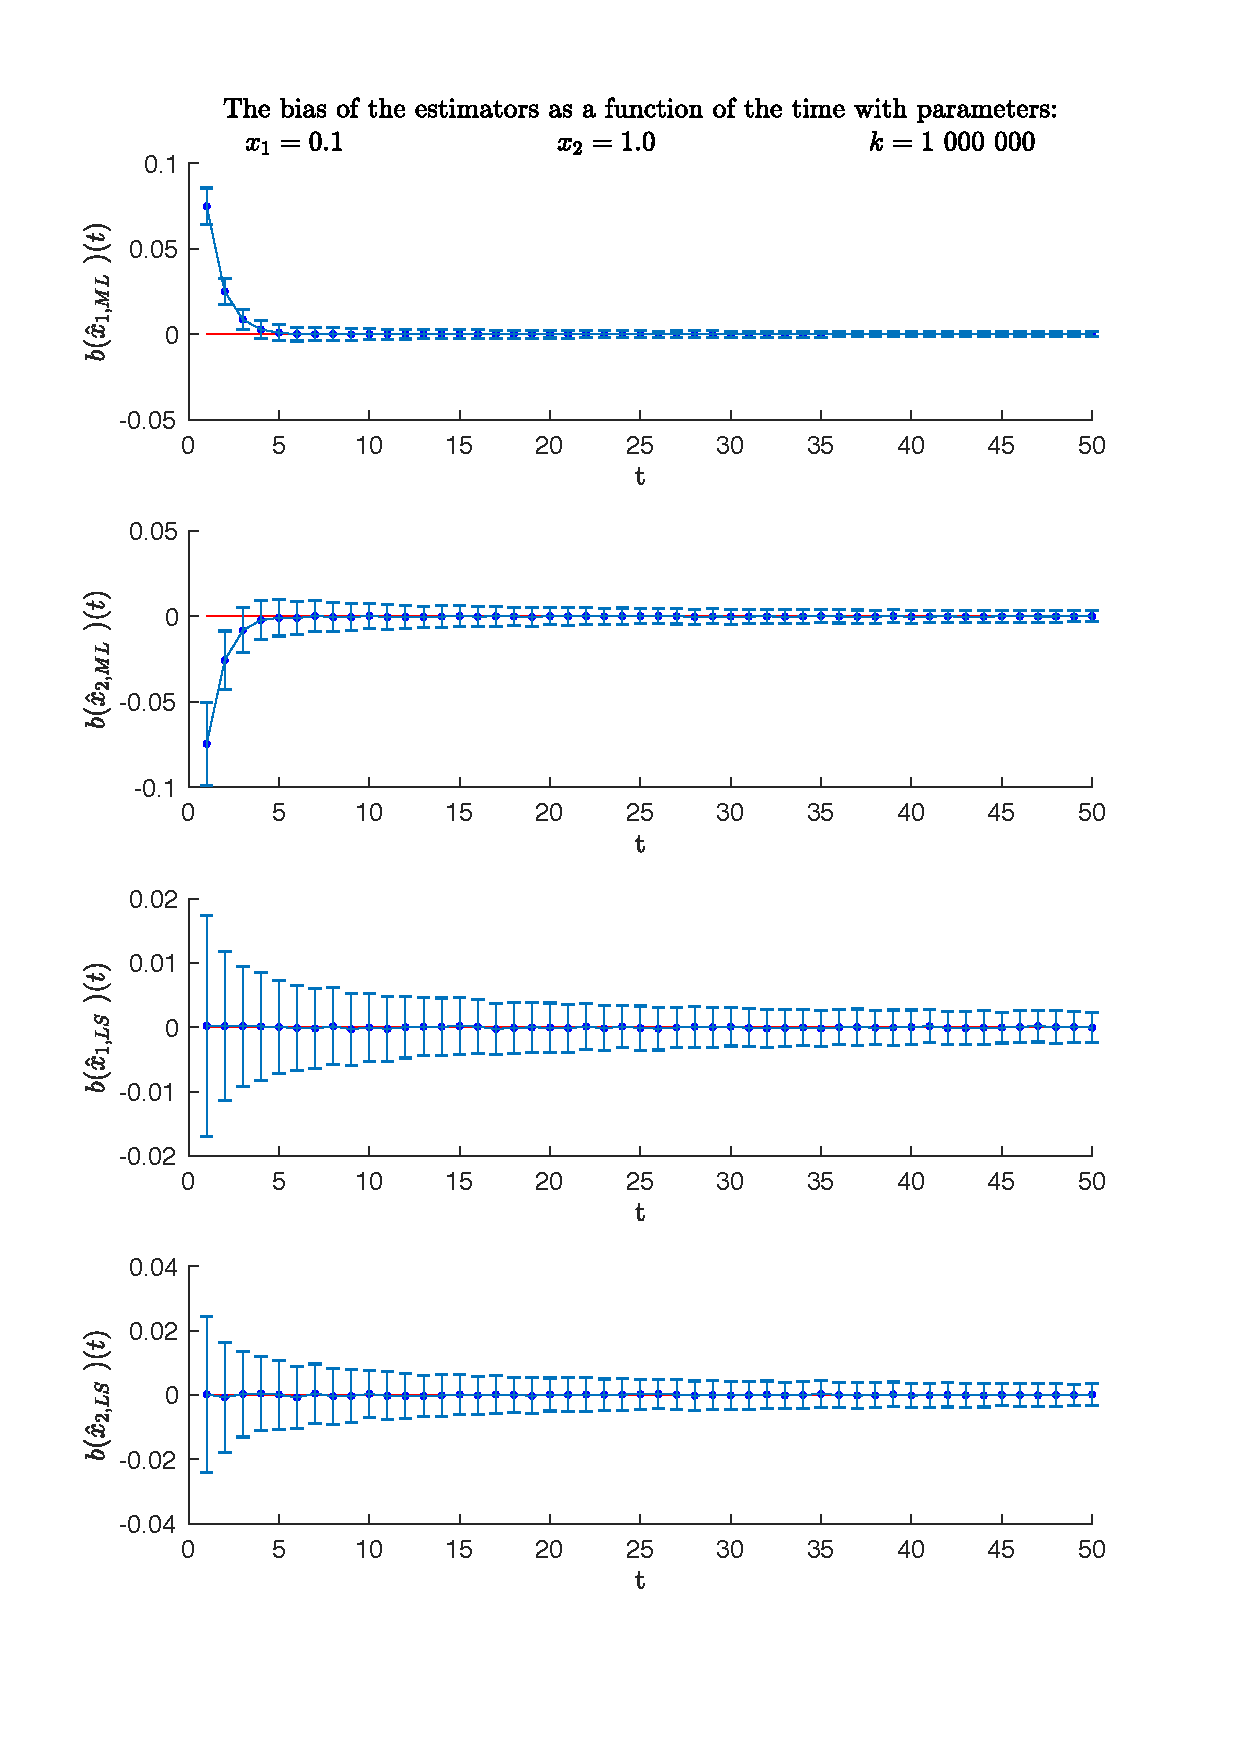
\includegraphics[width=\linewidth]{figures/BIasVsT}
	\caption{\emph{The bias of respectively the ML estimators $\hat x_{1,ml}$ and $\hat x_{2,ml}$, and the LS estimators $\hat x_{1,ls}$ and $\hat x_{2,ls}$. The error on the numerical estimation of all the biasses decreases as the time increases. As expected the ML estimators are biased for small values, but  asymptotically unbiased, while the LS estimators are always unbiased.}}
	\label{fig:biasToyProblem}
\end{figure}
\clearpage




%----------------------------------------------------------------------------
\subsection{Iterative reconstruction with MLEM}
The theory behind the MLEM iterative image reconstruction algorithm was studied in section \ref{sec:mlem}. Using the same simulated data as in the previous section, it is possible to test the MLEM algorithm. The MLEM algorithm is implemented in Matlab as
\begin{align}
	\hat x_{j}^{next} &= \frac{\hat x_{j}^{current}}{\sum_{i}a_{ij}}
	\sum_{i}a_{ij}
	\frac{y_{i}}{\sum_{k}a_{ik}\hat x_{k}^{current}}
\end{align}

The algorithm takes as parameters an initial guess for the image, the data, the system matrix and the desired number of iterations. It is then possible to run and test the algorithm.\\




\subsubsection*{Exact data}
The algorithm is first tested with a single simulation of exact data, which converges to an exact result and needs  only a few iterations before reaching a reasonable approximation. With $x_1 = 0.1,\ x_2 = 1$ and $t = 1$, the exact data is $y_1 = 0.1,\ y_2 = 1,\ y_3 = 1.1$, and the system matrix is the same as in the previous sections. Having no a priori information on the problem the initial guess is chosen to be $\hat x_1 = 1$ and $\hat x_2 = 1$. The iterative reconstruction using MLEM produces a rapidly converging series of estimators.\newline

\setlength\intextsep{0pt}
\begin{wraptable}{r}{5.5cm}
	\begin{tabular}{|r| l| l|}
		\hline
    	{Iteration nr.}	&${\hat x_1}$	&${\hat x_2}$\\
    	\hline
1 & 0.32500 & 0.77500\\ 
5 & 0.11406 & 0.98594\\ 
10 & 0.10044 & 0.99956\\ 
20 & 0.10000 & 1.00000\\ 
30 & 0.10000 & 1.00000\\ 
    	\hline
	\end{tabular}
	\caption{\emph{The convergence of the MLEM algorithm with a single exact data simulation. $x_1 = 0.1,\ x_2 = 1,\ t=1$.}}
    \label{tab:mlemExact}
\end{wraptable} 
\intextsep\skip32

It is clear that MLEM converges rapidly to the exact parameter values with exact data. In about 10 iterations a rather precise result is obtained, starting from a poor initial guess and convergence is achieved in less than 20 iterations.\\

The values of the ML estimators can be determined with eq. \ref{eq:toyMLComplete}. MLEM converges to these ML estimators. The ML estimators are for this setup
\begin{align} 
	\hat x_{1, ml} = \frac{y_1(y_1 + y_2 + y_3)}{2t(y_1 + y_2)} = 0.10000
	\nonumber\\
	%
	\hat x_{2, ml} = \frac{y_2(y_1 + y_2 + y_3)}{2t(y_1 + y_{2})} =1.00000  
	\nonumber
\end{align}

which combined with the results from table \ref{tab:mlemExact} confirms that MLEM converges to the ML estimators in this case. The convergence is represented graphically in figure \ref{fig:mlemconvergenceexact}.\\
\begin{figure}[H]
\begin{minipage}[c]{0.499\linewidth}
    \begin{figure}[H]
	\centering
	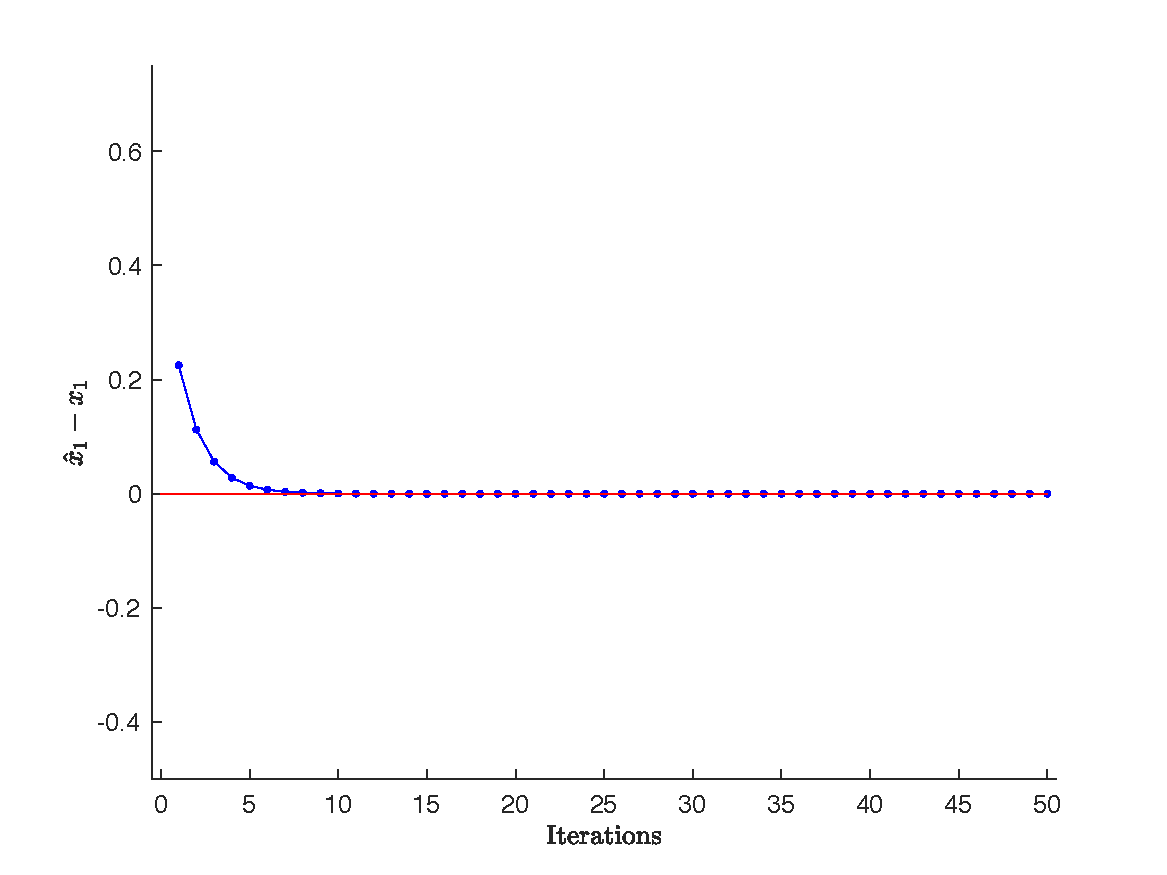
\includegraphics[width=\linewidth]{figures/MLEMConvergenceExact1}
	\end{figure}
\end{minipage}
\hfill
\begin{minipage}[c]{0.499\linewidth}
    \begin{figure}[H]
	\centering
	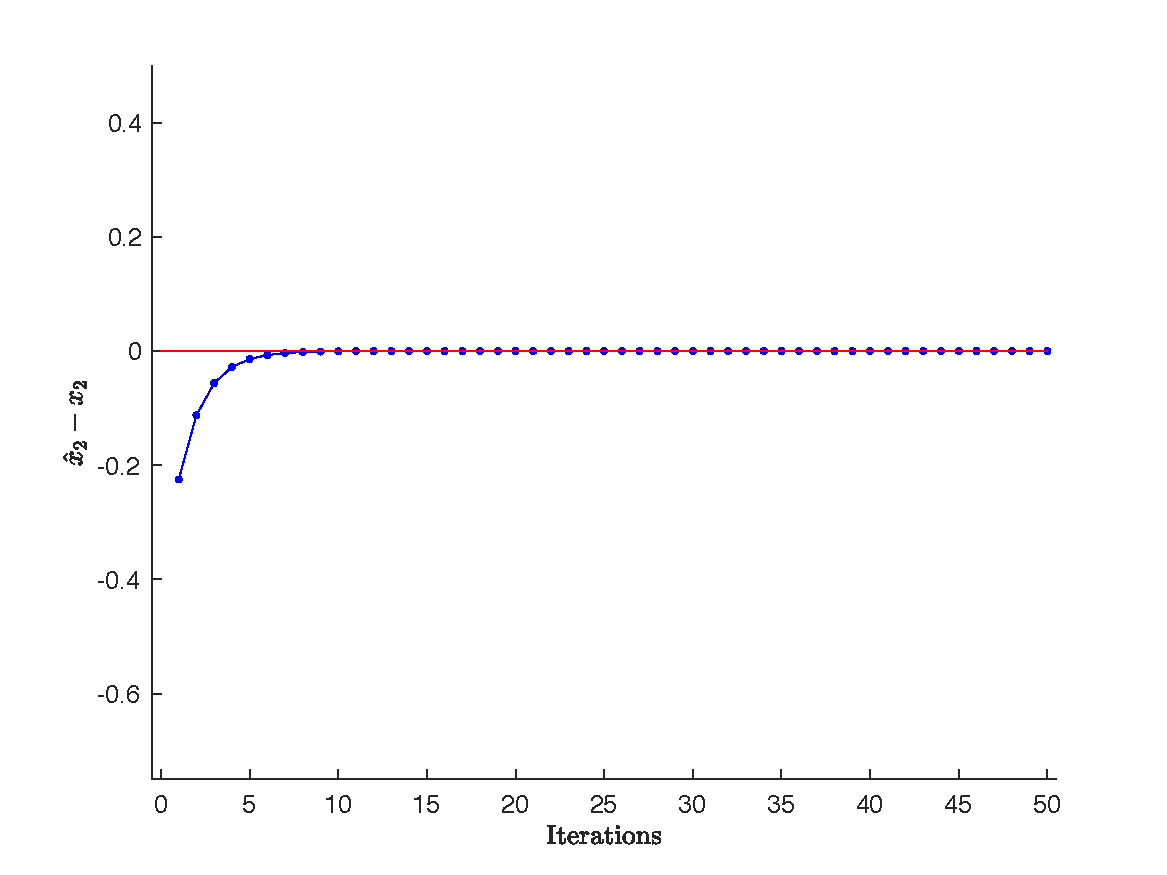
\includegraphics[width=\linewidth]{figures/MLEMConvergenceExact2}
\end{figure}
\end{minipage}
	\caption{\emph{The convergence of MLEM with a single simulation of exact data: $x_1 = 0.1,\ x_2 = 1,\ t = 1$. The value $\hat{x}_j - x_j$ is plotted to reflect simultaneously the convergence and the bias.}}
	\label{fig:mlemconvergenceexact}
\end{figure}




\subsubsection*{Noisy data} 
\begin{wraptable}{r}{6cm}
	\begin{tabular}{|r| l| l|}
		\hline
    	{Iteration nr.}	&${\hat x_1}$	&${\hat x_2}$\\
    	\hline
1 & 0.25000 & 1.25000\\ 
5 & 0.00309 & 1.49691\\ 
10 & 0.00001 & 1.49999\\ 
20 & 0.00000 & 1.50000\\ 
30 & 0.00000 & 1.50000\\ 
    	\hline
	\end{tabular}
	\caption{\emph{The convergence of MLEM with a single simulation of low count, Poisson distributed data. $x_1 = 0.1,\ x_2 = 1,\ t = 1$}}
    \label{tab:mlemNoisy}
\end{wraptable}
In a real world application, the data is always noisy. So if the data is assumed to be Poisson distributed around its true value, the MLEM algorithm behaves differently. Using again for the true value of the image $x_1 = 0.1,\ x_2 = 1$ and $t=1$, the data are Poisson random variables with $E[y_1] = 0.1,\ E[y_2] = 1,\ E[y_3] = 1.1$, and the system matrix is still the same as in the previous sections. The initial guess is again $\hat x_1 = \hat x_2 = 1$.

For this particular data simulation, the data is $y_1 = 0$, $y_2 = 1$ and $y_3 = 2$. Once again the algorithm converges rapidly though no longer to the exact parameter value. The ML estimators are for this particular data simulation
\begin{align} 
	\hat x_{1, ml} = \frac{y_1(y_1 + y_2 + y_3)}{2t(y_1 + y_2)} = 0.00000
	\nonumber\\
	%
	\hat x_{2, ml} = \frac{y_2(y_1 + y_2 + y_3)}{2t(y_1 + y_{2})} =1.50000  
	\nonumber
\end{align}

which shows again that MLEM converges as expected to the ML estimators. The convergence is represented graphically in figure \ref{fig:mlemconvergencenoisylowdata}.\\
\begin{figure}[H]
\begin{minipage}[c]{0.499\linewidth}
    \begin{figure}[H]
	\centering
	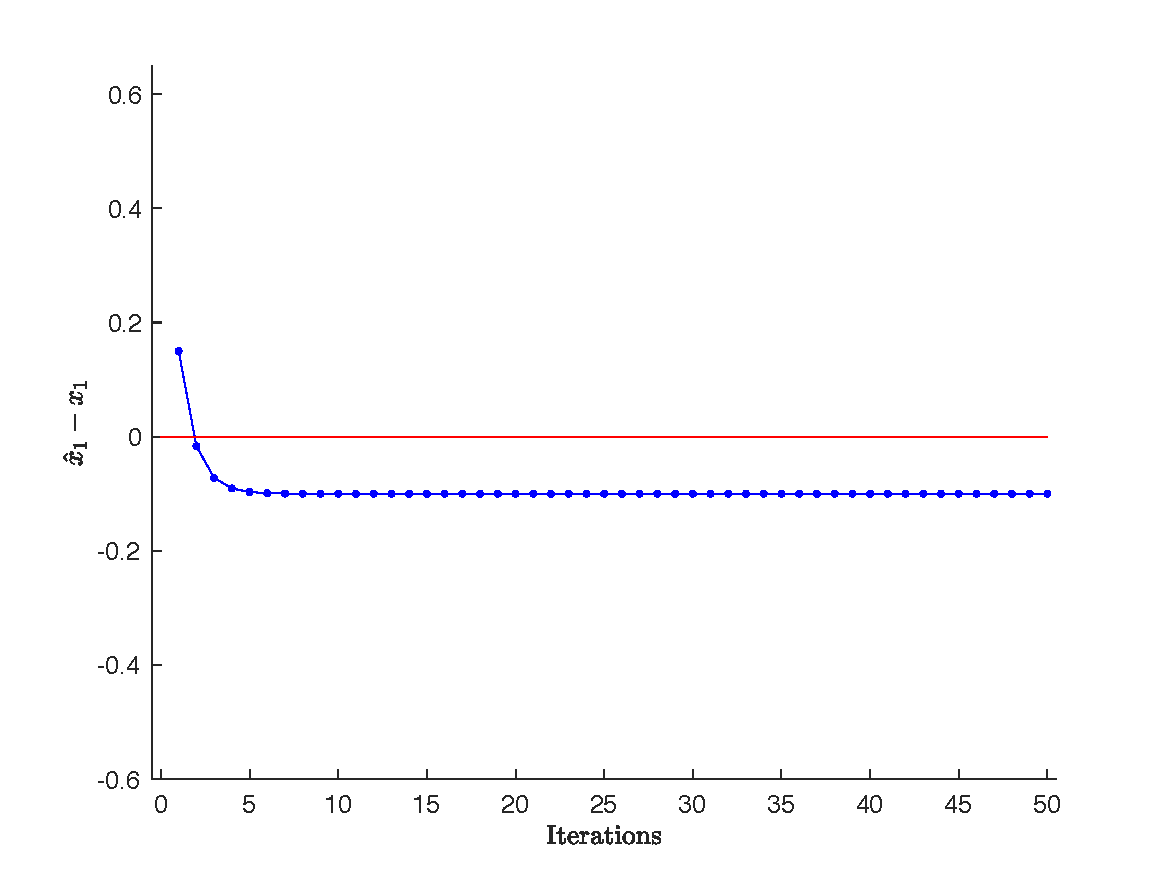
\includegraphics[width=\linewidth]{figures/MLEMConvergenceLow1}
	\end{figure}
\end{minipage}
\hfill
\begin{minipage}[c]{0.499\linewidth}
    \begin{figure}[H]
	\centering
	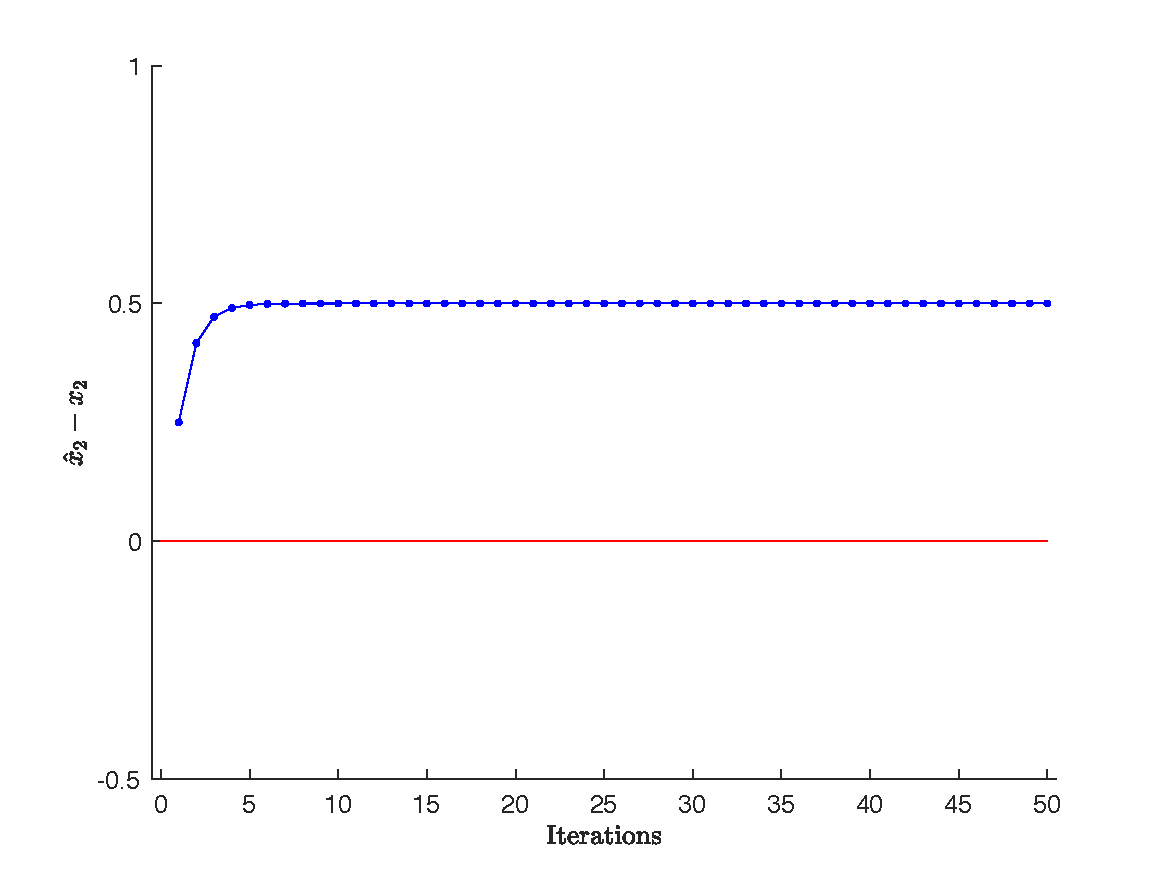
\includegraphics[width=\linewidth]{figures/MLEMConvergenceLow2}
\end{figure}
\end{minipage}
	\caption{\emph{The convergence of MLEM with a single simulation of low count, Poisson distributed data. $x_1 = 0.1, x_2 = 1, t = 1$. With noisy, low count data MLEM produces a biassed estimate.\\}}
	\label{fig:mlemconvergencenoisylowdata}
\end{figure}



The previous figures \ref{fig:mlemconvergenceexact} and \ref{fig:mlemconvergencenoisylowdata} were obtained with low data counts. In this limit ML estimators are known to be biassed. ML estimators are also known to be asymptotically unbiassed.\\

 To verify the asymptotic behaviour, a simulation can be performed with high data counts. This can be achieved by increasing the activities in the image pixels or by increasing the measurement time. With the same setup as before ($x_1 = 0.1,\ x_2 = 1$) but increasing the measurement time $t = 1$ to $t = 50$ produces a better estimation. This estimation's convergence is represented graphically in figure \ref{fig:mlemconvergencenoisyhighdata}\\
\begin{figure}[H]
\begin{minipage}[c]{0.499\linewidth}
    \begin{figure}[H]
	\centering
	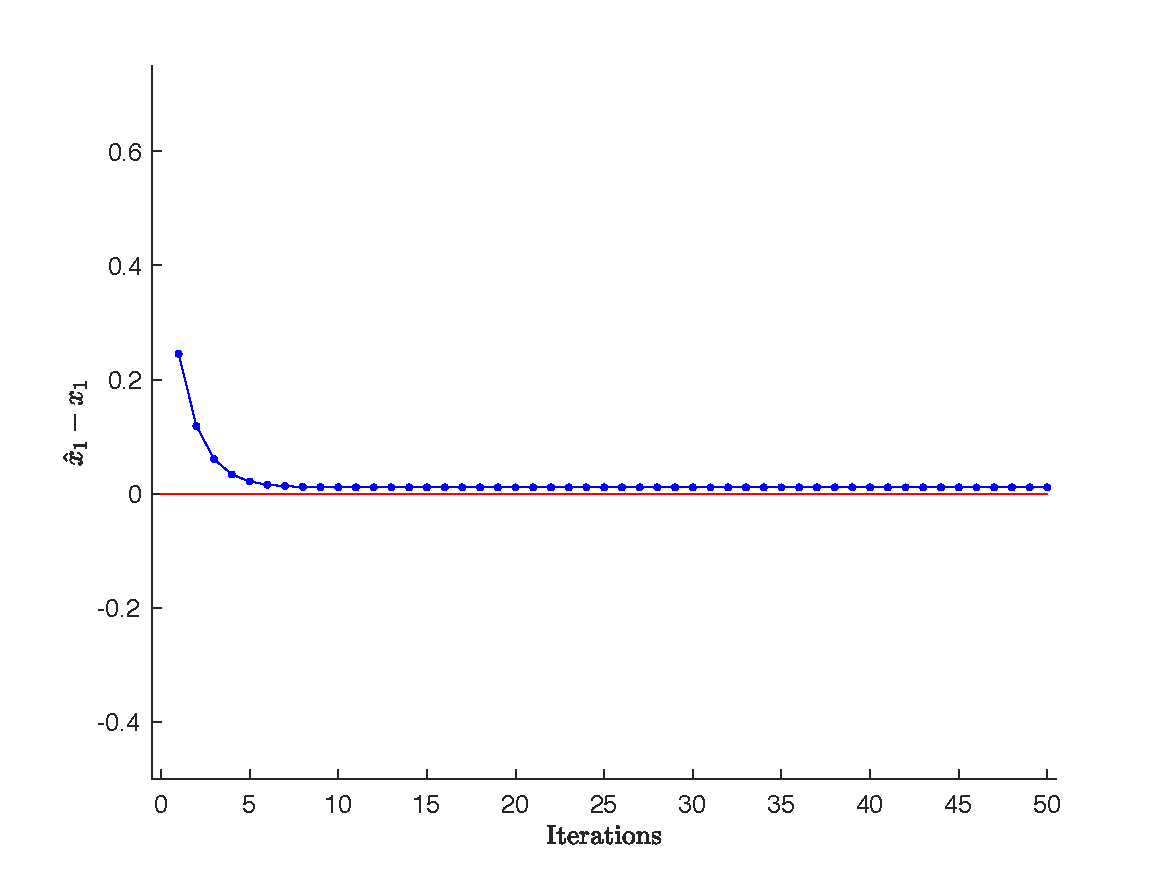
\includegraphics[width=\linewidth]{figures/MLEMConvergenceHigh1}
	\end{figure}
\end{minipage}
\hfill
\begin{minipage}[c]{0.499\linewidth}
    \begin{figure}[H]
	\centering
	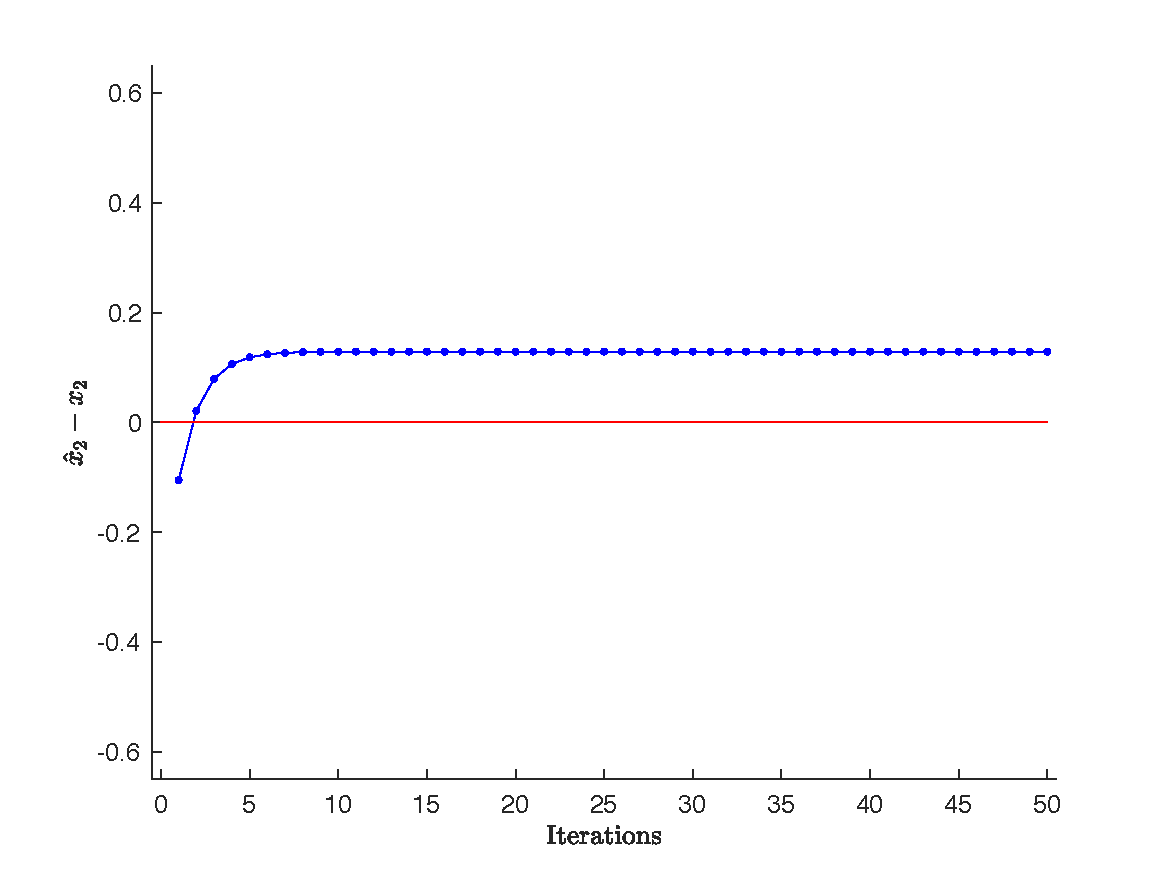
\includegraphics[width=\linewidth]{figures/MLEMConvergenceHigh2}
\end{figure}
\end{minipage}
	\caption{\emph{The convergence of MLEM with a single simulation of high count, Poisson distributed data. $x_1 = 0.1, x_2 = 1, t = 50$. With high count data MLEM produces estimators with a smaller bias, compared to low count data.}}
	\label{fig:mlemconvergencenoisyhighdata}
\end{figure}












%----------------------------------------------------------------------------
\subsection{Iterative reconstruction with ISRA}
\setlength\intextsep{0pt}
\begin{wraptable}{r}{6cm}
	\begin{tabular}{|r| l| l|}
		\hline
    	{Iteration nr.}	&${\hat x_1}$	&${\hat x_2}$\\
    	\hline
1 & 0.40000 & 0.70000\\ 
5 & 0.19817 & 0.93475\\ 
10 & 0.13710 & 0.97761\\ 
25 & 0.10430 & 0.99753\\ 
50 & 0.10017 & 0.99990\\ 
100 & 0.10000 & 1.00000\\ 
    	\hline
	\end{tabular}
	\caption{\emph{The convergence of ISRA with a single simulation of exact data. $x_1 = 0.1,\ x_2 = 1,\ t=1$.}}
    \label{tab:israExact}
\end{wraptable}
Using ISRA to iteratively reconstruct the image is yet another possible method for estimating the image. The ISRA algorithm was studied in section \ref{sec:isra}. It takes as parameters an initial guess for the image, the data, the system matrix and the desired number of iterations. It is then possible to run and test the algorithm. ISRA is implemented in Matlab as\\ \\
\begin{align}
	\hat x_j^{next} = \hat x_j^{current}\frac
	{\sum_{i} a_{ij}y_i}
	{\sum_{k} \sum_{l} a_{kj}a_{kl}x_l^{current}}\ \  i = 1,\ ...\ ,n
\end{align}






\subsubsection*{Exact data}
The first test uses a single exact data simulation. The parameters are $x_1 = 0.1$, $x_2 = 1.0$, $t = 1$ and exact data is $y_1 = 0.1$, $y_2 = 1.0$ and $y_3 = 1.1$. The initial guess is again $\hat x_1 = \hat x_2 = 1$. Table \ref{tab:israExact} shows that ISRA converges to the exact parameter values, but needs significantly more iterations than MLEM to converge.\\

ISRA is expected to converge to constrained non-negative LS estimators. The unconstrained LS estimators are given by \ref{eq:lsestiators} and are for this simulation
\begin{align}
	\hat x_{1, ls} = \frac{(2 y_1 - y_2 + y_3)}{3t} = 0.10000\nonumber\\
	\hat x_{2, ls } = \frac{(2 y_2 - y_1 + y_3)}{3t} = 1.00000\nonumber
\end{align}

which shows that in this noiseless case ISRA converges to the exact parameter values which are equal to the LS estimators. The convergence is represented graphically in figure \ref{fig:israconvergenceexactdata}\\
\begin{figure}[H]
\begin{minipage}[c]{0.499\linewidth}
    \begin{figure}[H]
	\centering
	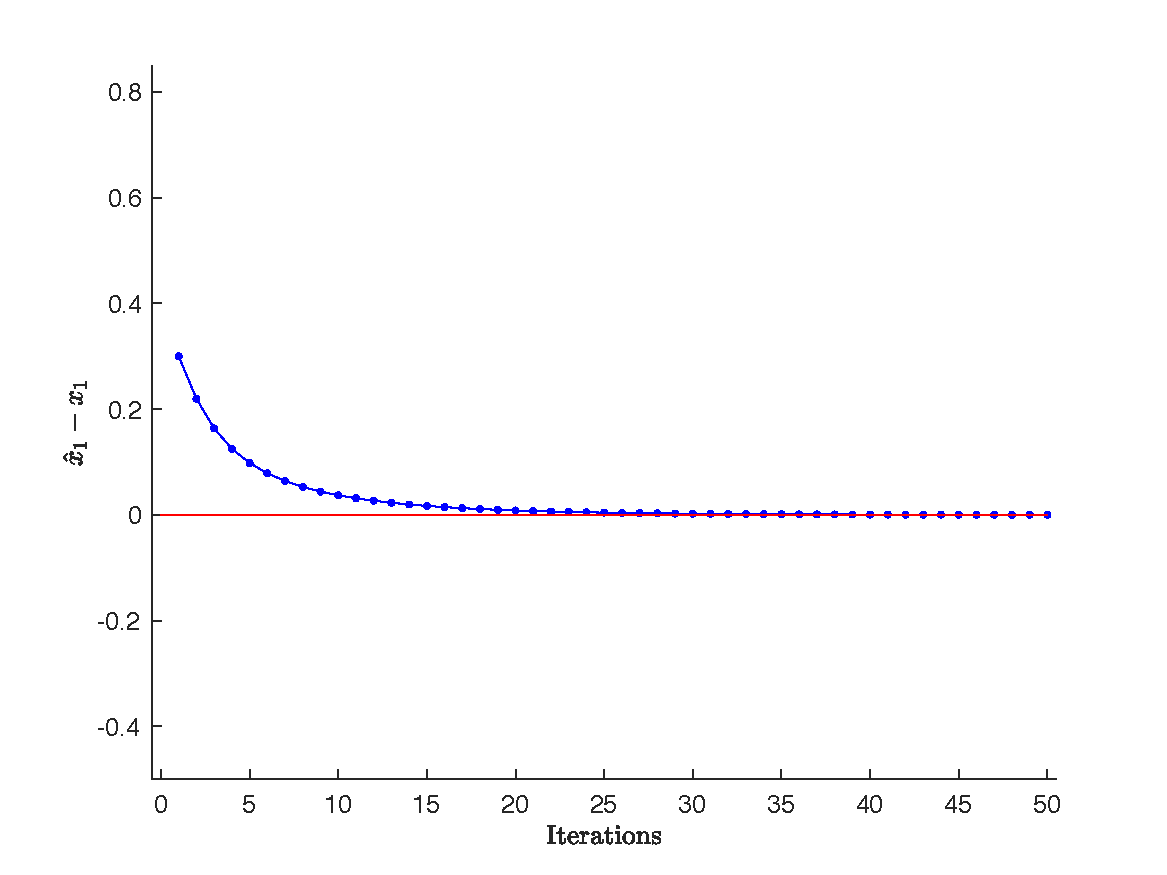
\includegraphics[width=\linewidth]{figures/ISRAConvergenceExact1}
	\end{figure}
\end{minipage}
\hfill
\begin{minipage}[c]{0.499\linewidth}
    \begin{figure}[H]
	\centering
	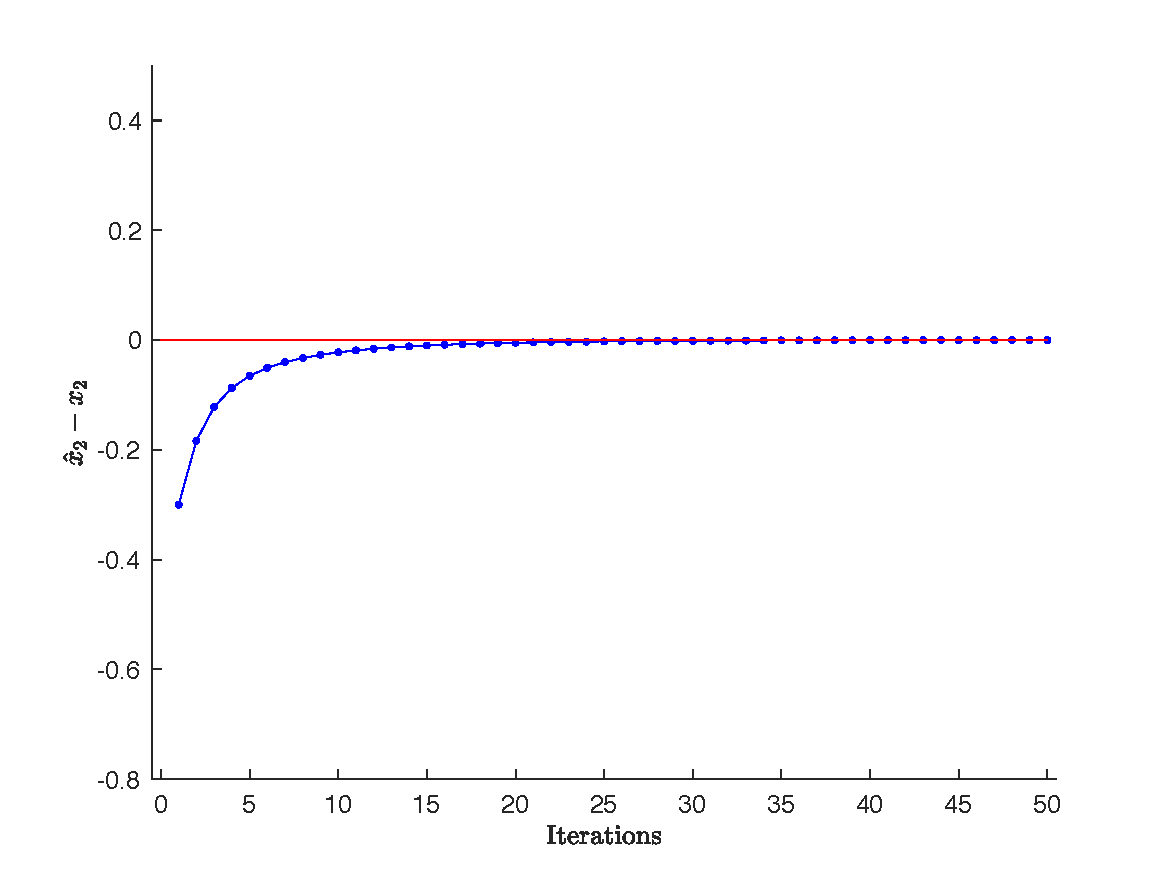
\includegraphics[width=\linewidth]{figures/ISRAConvergenceExact2}
\end{figure}
\end{minipage}
    \caption{\emph{The convergence of ISRA with a single simulation of exact data. $x_1 = 0.1,\ x_2 = 1,\ t = 1$.}}
    \label{fig:israconvergenceexactdata}
\end{figure}








\subsubsection*{Noisy data}
\setlength\intextsep{0pt}
\begin{wraptable}{r}{6cm}
	\begin{tabular}{|r| l| l|}
		\hline
    	{Iteration nr.}	&${\hat x_1}$	&${\hat x_2}$\\
    	\hline
1 & 0.66667 & 1.00000\\ 
5 & 0.42467 & 1.26632\\ 
10 & 0.35608 & 1.31782\\ 
25 & 0.33383 & 1.33300\\ 
50 & 0.33333 & 1.33333\\
    	\hline
	\end{tabular}
		\caption{\emph{The convergence of ISRA with a single simulation of low count, Poisson distributed data. $x_1 = 0.1$, $x_2 = 1.0$, $t = 1$}}
    \label{tab:isranoisy1}
   \end{wraptable}
ISRA is also tested on noisy data. The setup is $x_1 = 0.1$, $x_2 = 1.0$ and $t = 1$. The data are then Poisson random variables with $E[y_1] = 0.1, E[y_2] = 1.0$ and $E[y_3] = 1.1$. The initial guess is again $\hat x_1 = \hat x_2 = 1$.\\

Data is simulated 2 times. The data produced for the first simulation is $y_1=0$, $y_2=1$, $y_3=2$.\\ 

Applying ISRA on this noisy data produces the series of estimators in table \ref{tab:isranoisy1}. As expected ISRA converges rapidly, but not to the exact parameter values. The unconstrained LS estimators are for this simulation
    \begin{align}
    	\hat x_{1,ls} & = \frac{(2 y_1 - y_2 + y_3)}{3t} = 0.33333...\nonumber\\
    	\hat x_{2,ls} & = \frac{(2 y_2 - y_1 + y_3)}{3t} = 1.33333...\nonumber
    \end{align}

which shows that in this case ISRA converges to the unconstrained LS estimators.\\

A second simulation is performed with the same parameters, but a different noise realisation to see whether ISRA always converges to the unconstrained LS estimators. The data produced for the second simulation is $y_1=0$, $y_2=4$, $y_3=2$. The LS estimators are then
\begin{align}
	\hat x_{1,ls} &= -0.66666...\nonumber\\
	\hat x_{2,ls} &= 3.33333...\nonumber
\end{align}

\setlength\intextsep{0pt}
\begin{wraptable}{r}{6cm}
    	\begin{tabular}{|r| l| l|}
		\hline
    	{Iteration nr.}	&${\hat x_1}$	&${\hat x_2}$\\
    	\hline
1 & 0.66667 & 2.00000\\ 
5 & 0.09194 & 2.92594\\ 
10 & 0.01104 & 2.99165\\ 
25 & 0.00002 & 2.99998\\ 
50 & 0.00000 & 3.00000\\ 
    	\hline
	\end{tabular}
	\caption{\emph{The convergence of ISRA with a different simulation of low count, Poisson distributed data. $x_1 = 0.1$, $x_2 = 1.0$, $t = 1$}}
    \label{tab:isranoisy2}
\end{wraptable}
In general LS estimators can be negative but ISRA has a positivity constraint and can only generate non-negative images (assuming a non-negative initial guess). It is therefore to be expected that ISRA does converge to the constrained non-negative LS estimators but not to the unconstrained estimators. This is confirmed by comparing the LS estimators with the series of estimators produced by ISRA for this particular noise simulation found in table \ref{tab:isranoisy2}.\\

The convergence of ISRA with noisy data is also  represented graphically in figure \ref{fig:israconvergencelownoise}. Again the effect of adding more data by increasing the measurement time can be made apparent by simulating with $t = 50$ instead of $t=1$. This effect is represented in figure \ref{fig:israconvergencehighnoise}.
\setlength\intextsep{\savedintextsep}
\begin{figure}[H]
	\begin{minipage}[c]{0.499\linewidth}
    \begin{figure}[H]
	\centering
	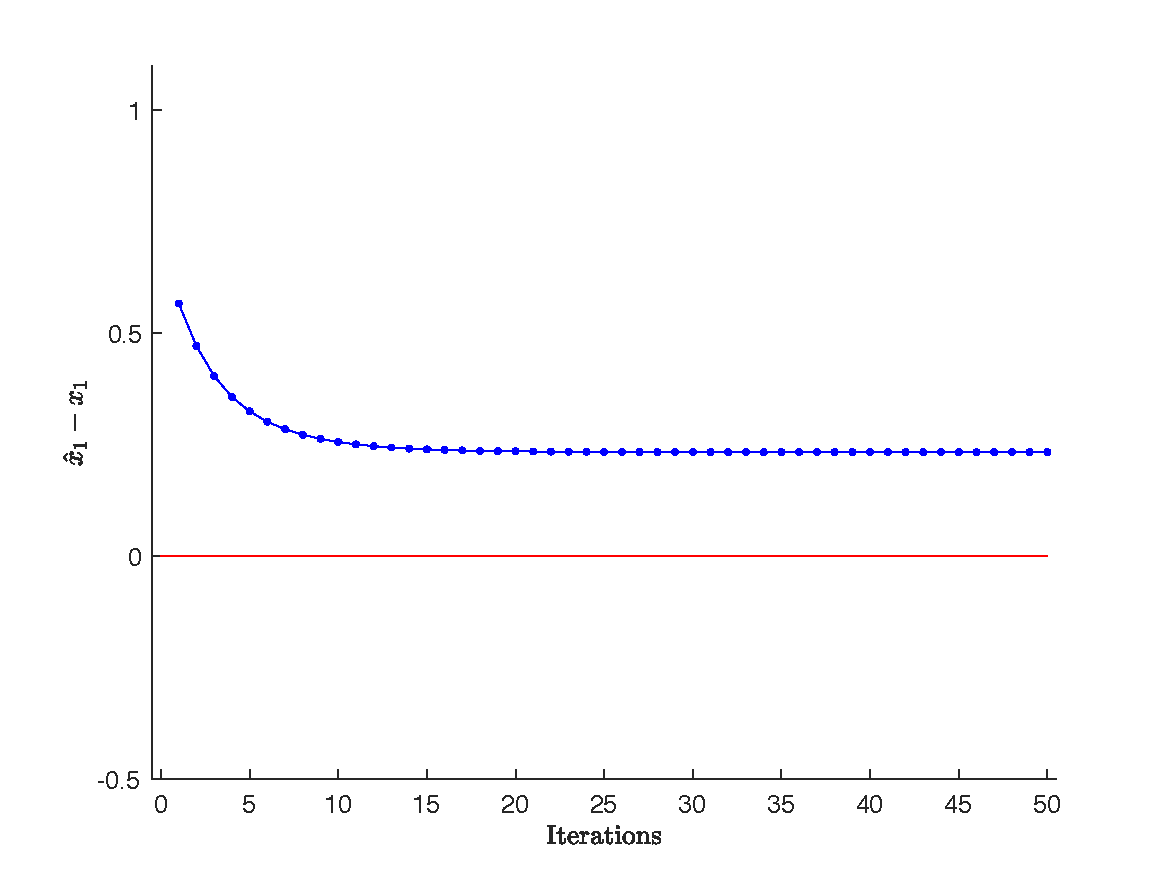
\includegraphics[width=\linewidth]{figures/ISRAConvergenceLow1}
	\end{figure}
\end{minipage}
\hfill
\begin{minipage}[c]{0.499\linewidth}
    \begin{figure}[H]
	\centering
	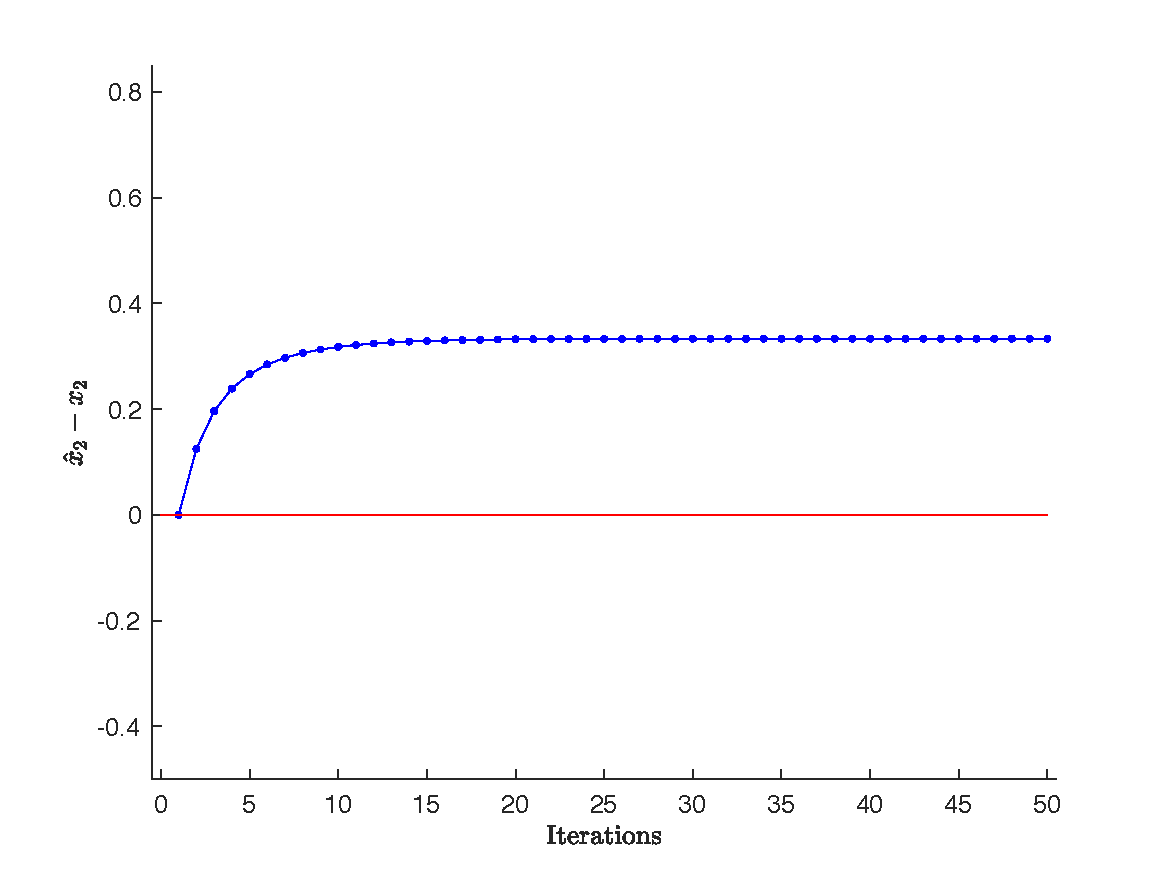
\includegraphics[width=\linewidth]{figures/ISRAConvergenceLow2}
\end{figure}
\end{minipage}
    \caption{\emph{The convergence of ISRA with a single simulation of low count, Poisson distributed data. $x_1 = 0.1, x_2 = 1, t = 1$}}
    \label{fig:israconvergencelownoise}
\end{figure}

\begin{figure}[H]
	\begin{minipage}[c]{0.499\linewidth}
    \begin{figure}[H]
	\centering
	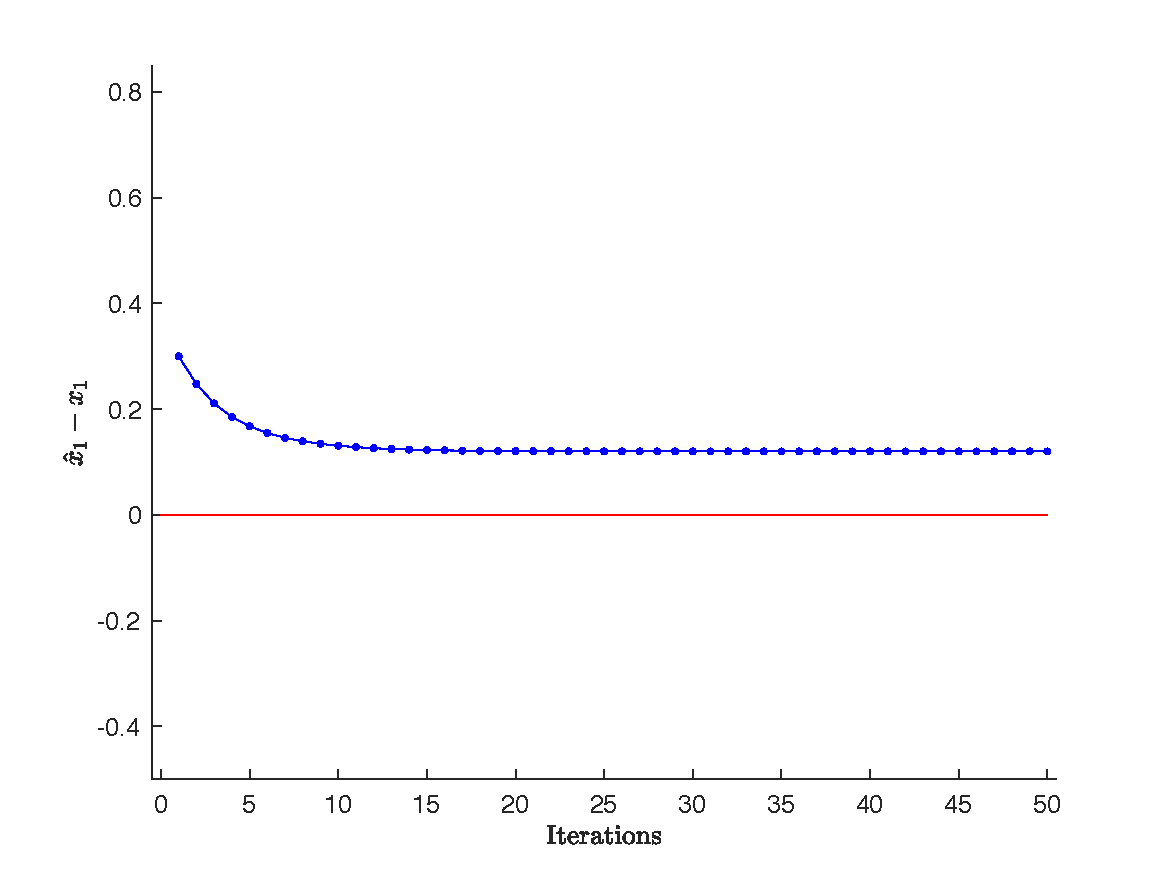
\includegraphics[width=\linewidth]{figures/ISRAConvergenceHigh1}
	\end{figure}
\end{minipage}
\hfill
\begin{minipage}[c]{0.499\linewidth}
    \begin{figure}[H]
	\centering
	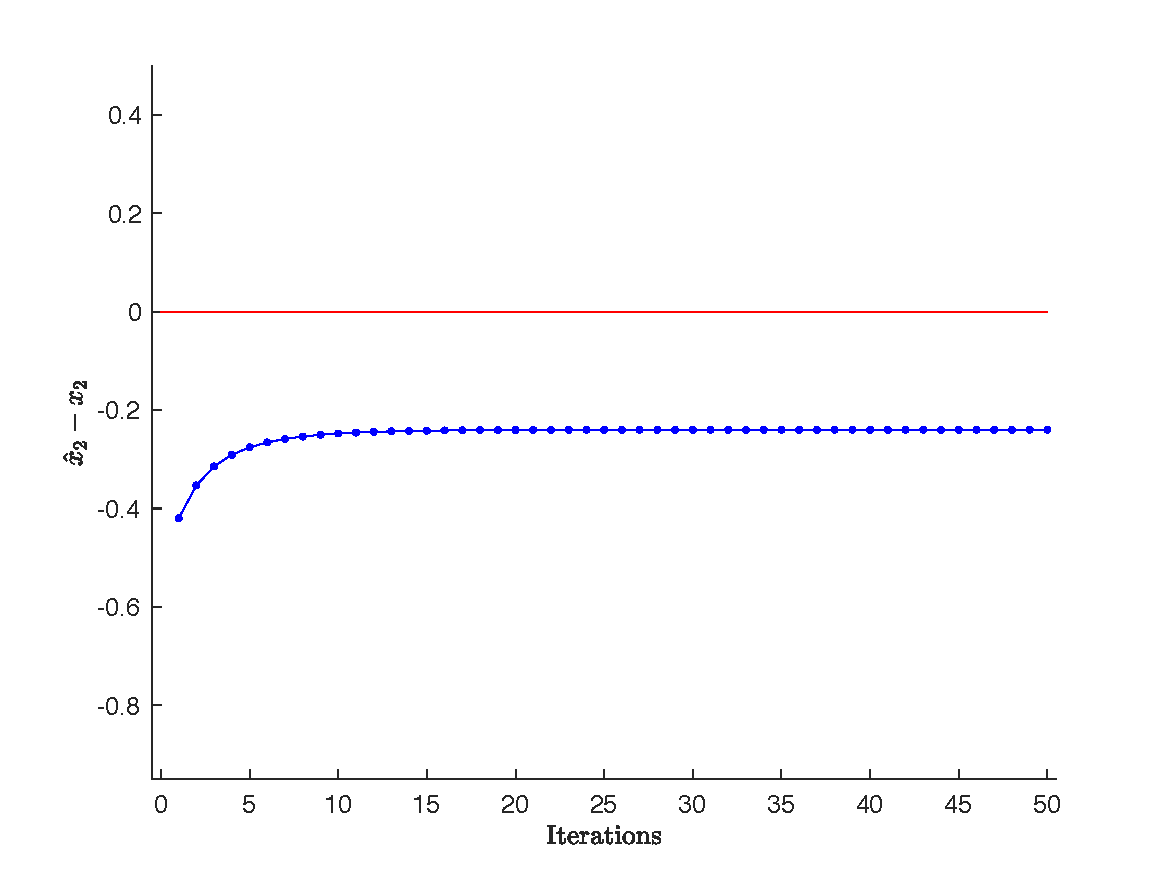
\includegraphics[width=\linewidth]{figures/ISRAConvergenceHigh2}
\end{figure}
\end{minipage}
    \caption{\emph{The convergence of ISRA with a single simulation of high count, Poisson distributed data. $x_1 = 0.1, x_2 = 1, t = 50$}}
    \label{fig:israconvergencehighnoise}
\end{figure}

The previous discussions based every time on a single data simulation gave some feeling of the behaviour of ISRA. The fundamental questions that remain to be answered are whether ISRA systematically converges to the unconstrained LS estimators when enough data is available and how the bias of ISRA behaves as a function of the time $t$ and therefore as a function of the amount of data.\\

To verify that ISRA systematically converges to the unconstrained LS estimators when enough data is available, ISRA is used to reconstruct 100 000 toy problem simulations with parameters $x_1 = 0.1, x_2 = 1$ and $t = 1000$. For each reconstruction, the LS estimators and the ISRA estimators after 100 iterations were equal up to at least 5 digits after the decimal point. The conclusion is that ISRA used on high count data converges to the unconstrained, unbiassed LS estimators. This can also be seen asymptotically in figure \ref{fig:israbias}.\\

The other question is how ISRA's estimators' biasses behave. The biasses of the LS estimators were already studied in figure \ref{fig:biasToyProblem}. Because ISRA converges to the constrained non-negative LS estimators, the bias is expected to behave differently, and especially in the low count case. Figure \ref{fig:israbias} shows that ISRA produces biassed estimators which converge asymptotically to the unconstrained, unbiassed LS estimators if the amount of data is large enough. At each time $t$, 10000 data simulations are performed which allow determining the expected value and the bias of the ISRA estimators and the LS estimators.\\

There are several important conclusions for the iterative reconstruction algorithms MLEM and ISRA:
\begin{itemize}
	\item MLEM converges to unconstrained ML estimators.
	
	\item MLEM produces asymptotically unbiassed estimators because the ML estimators are asymptotically unbiassed.
	
	\item ISRA converges to constrained non-negative LS estimators.
	
	\item ISRA produces asymptotically unbiassed estimators because ISRA converges asymptotically to unconstrained LS estimators, which are unbiassed.
	
	\item MLEM converges faster than ISRA for the toy problem.
	
	\item The 'quality  of reconstruction' can be improved by increasing the amount of data. This can be done by increasing the activity in the pixels or by increasing the measurement time. Biologically increasing the measurement time is the more sensible method for increasing the quality.
\end{itemize}
\begin{figure}[H]
	\begin{minipage}[c]{.499\linewidth}
    \begin{figure}[H]
	\centering
	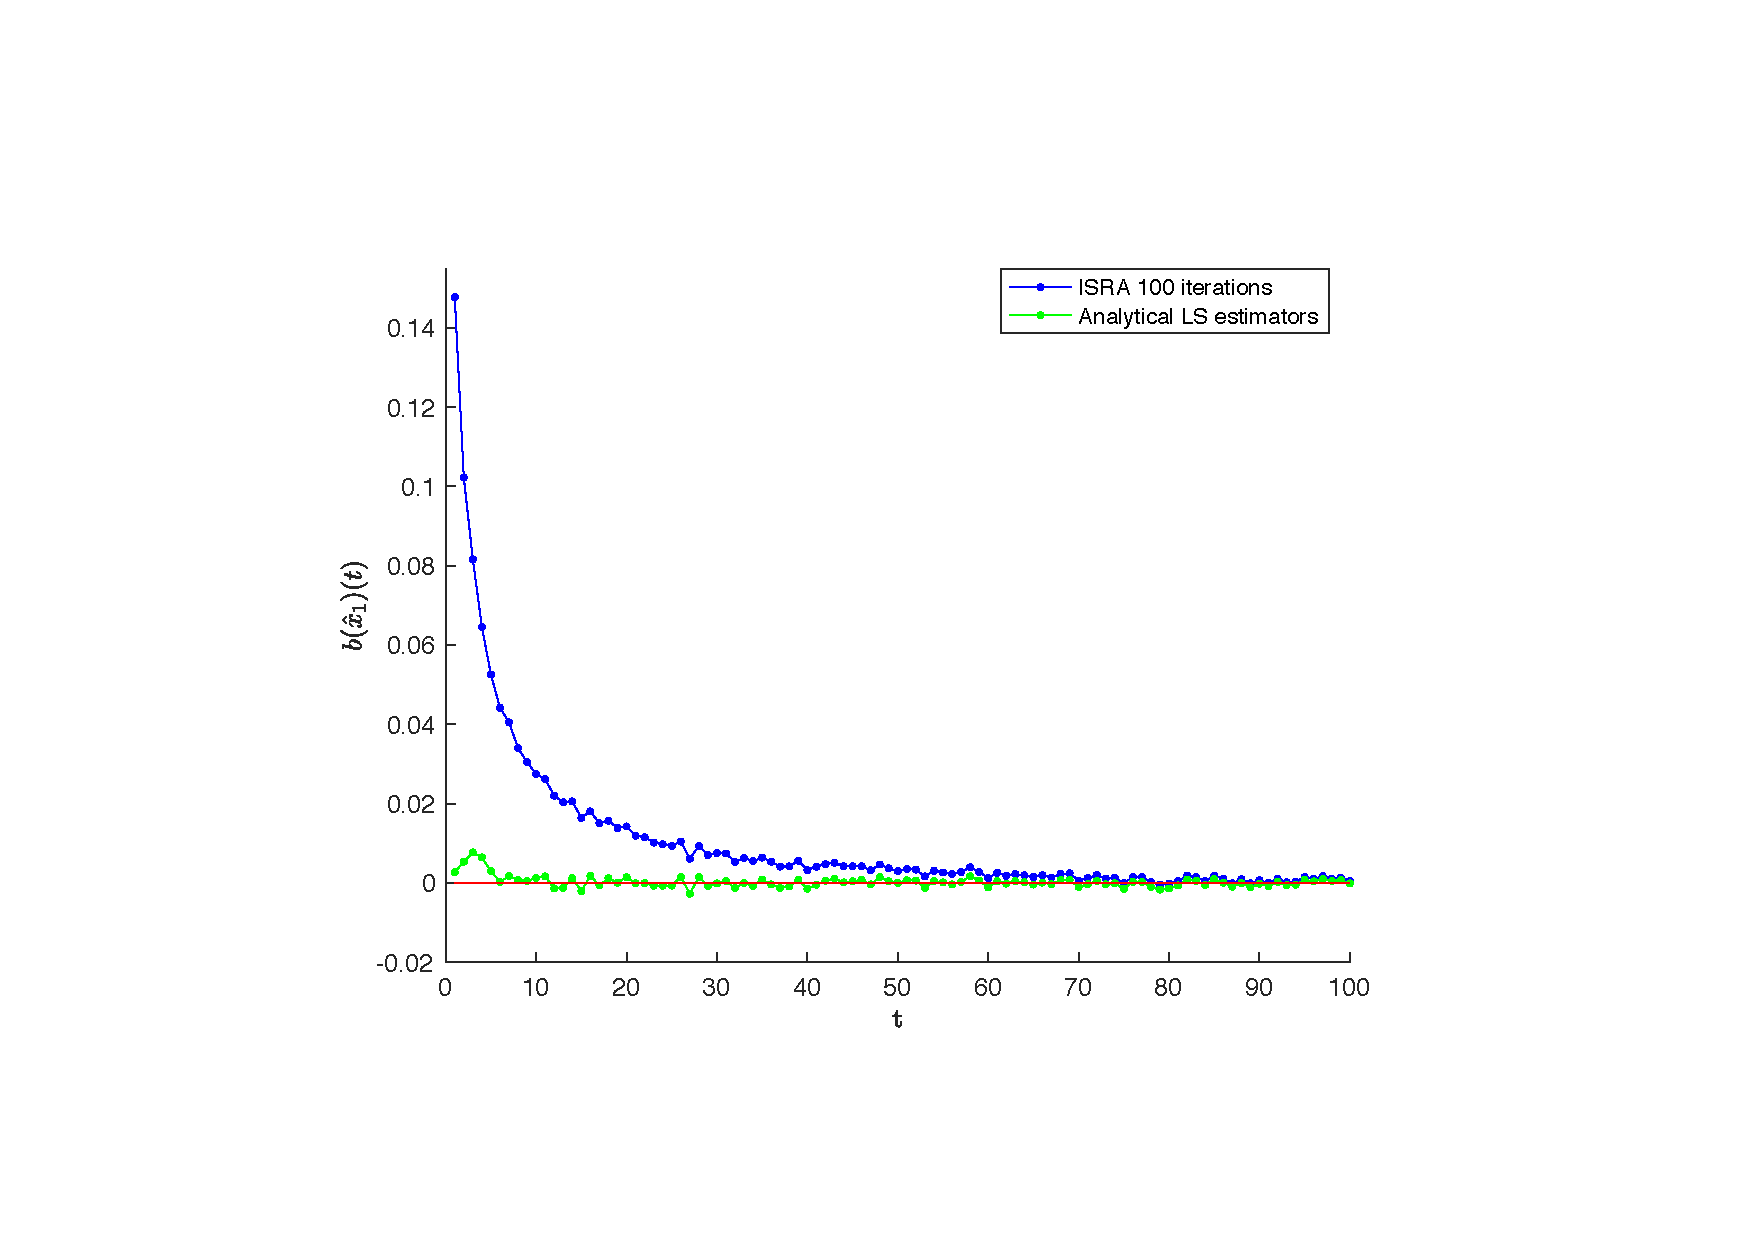
\includegraphics[width=\linewidth]{figures/ISRABiasVsT1}
	\end{figure}
\end{minipage}
\hfill
\begin{minipage}[c]{.499\linewidth}
    \begin{figure}[H]
	\centering
	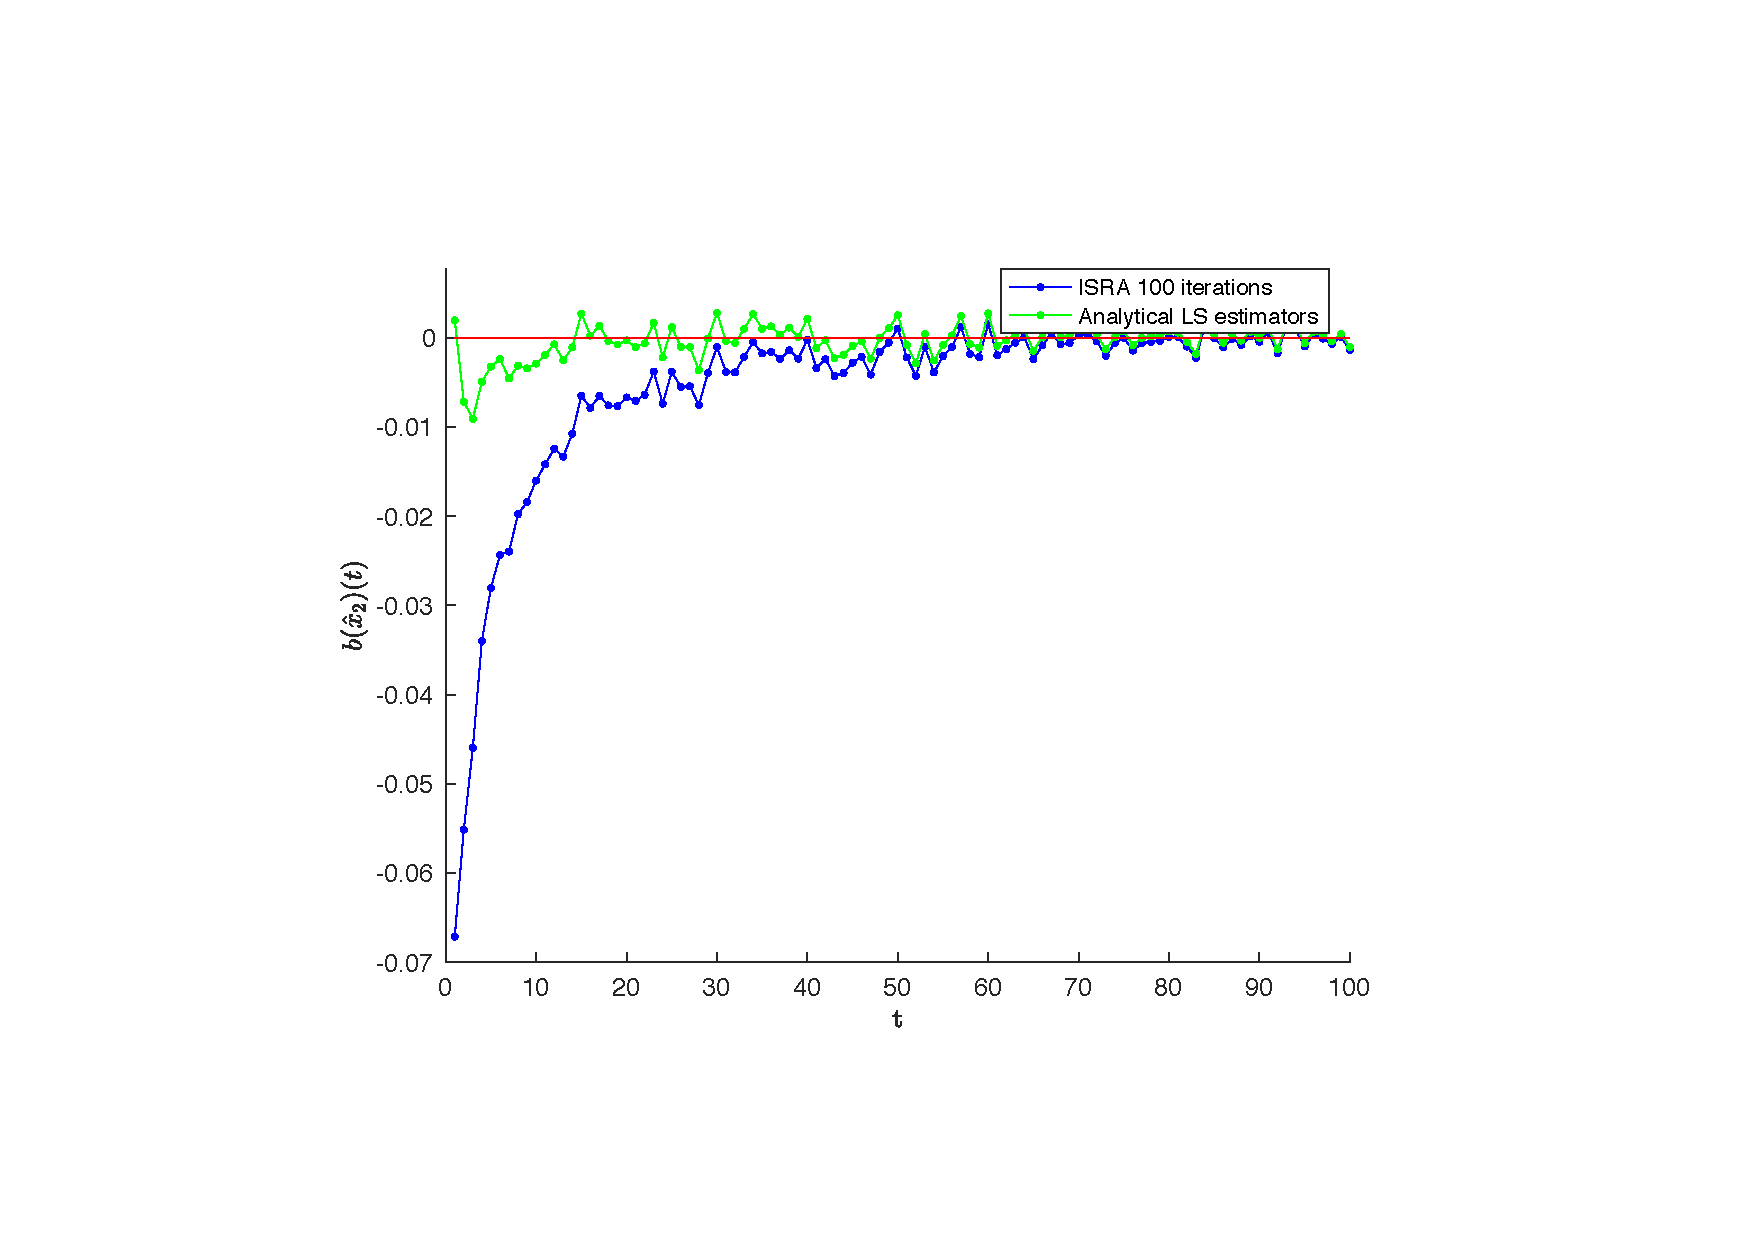
\includegraphics[width=\linewidth]{figures/ISRABiasVsT2}
\end{figure}
\end{minipage}
	\caption{\emph{The bias of the estimators produced by ISRA after $100$ iterations with parameters $x_1 = 0.1, x_2 = 1.0, t = 1 \rightarrow 100$ is compared to the corresponding bias on the unconstrained LS estimators.}}
	\label{fig:israbias}
\end{figure}


%----------------------------------------------------------------------------
%Chapter 3: MLEM-vs-ISRA
%----------------------------------------------------------------------------
\chapter{Study of PET reconstruction methods: MLEM vs. ISRA}\label{chpt:PETRecMethods}
\chaptermark{Study of PET reconstruction methods}
Different analytical and statistical methods to reconstruct an image from PET-data have been derived and studied. These methods were tested on a small problem to have some feeling for their behaviour and to allow the derivation of exact closed form expressions. This chapter will further study the iterative reconstruction algorithms MLEM and ISRA, and study and compare their properties on realistic data.\\

Historically ISRA was developed to be used in 3D volume PET reconstruction problems. In a true 3D reconstruction, the amount of LORs increases dramatically since cross-slice LORs are also used. This leads to an enormous, but sparsely populated data array. It is computationally not easy to reconstruct this data using MLEM due to excessive memory requirements or frequent and slow disk read/write operations. By backprojecting the data first to the 3D volume image as in ISRA, the memory requirements are significantly reduced. An additional benefit of backprojecting the data only once is that the amount of work to be done at each iteration is reduced, producing a faster algorithm.\\

The PET-data and the true image are generated by a PET-simulator. The image consists of several objects (cylinders, ellipsoids, Gaussians, cones or elliptical cylinders) where each object has a certain value for the activity in that object.

The image that will be discussed in detail is a Jaszczak 
phantom\footnote{A Jaszczak phantom is device that is used to test and calibrate PET-scanners. It consists of several containers that can be filled with either a tracer liquid or inert water, thus creating different regions with possibly different activities. All dimensions and activity values of the phantom are known and it can therefore be used for calibration.} \cite{Jaszczak} with 25 hot regions of varying size with activity = 2, 23 cold regions of varying size with no activity and a constant background with activity = 1. The image is 512 pixels wide and 512 pixels high. Each pixel has sides of 0.1 mm.\\

The MLEM and ISRA algorithm are implemented and are used to reconstruct the image. The aim of this chapter is to compare their different properties and in particular the bias and the variance.
\begin{figure}[H]
\begin{minipage}[c]{0.499\linewidth}
    \begin{figure}[H]
	\centering
	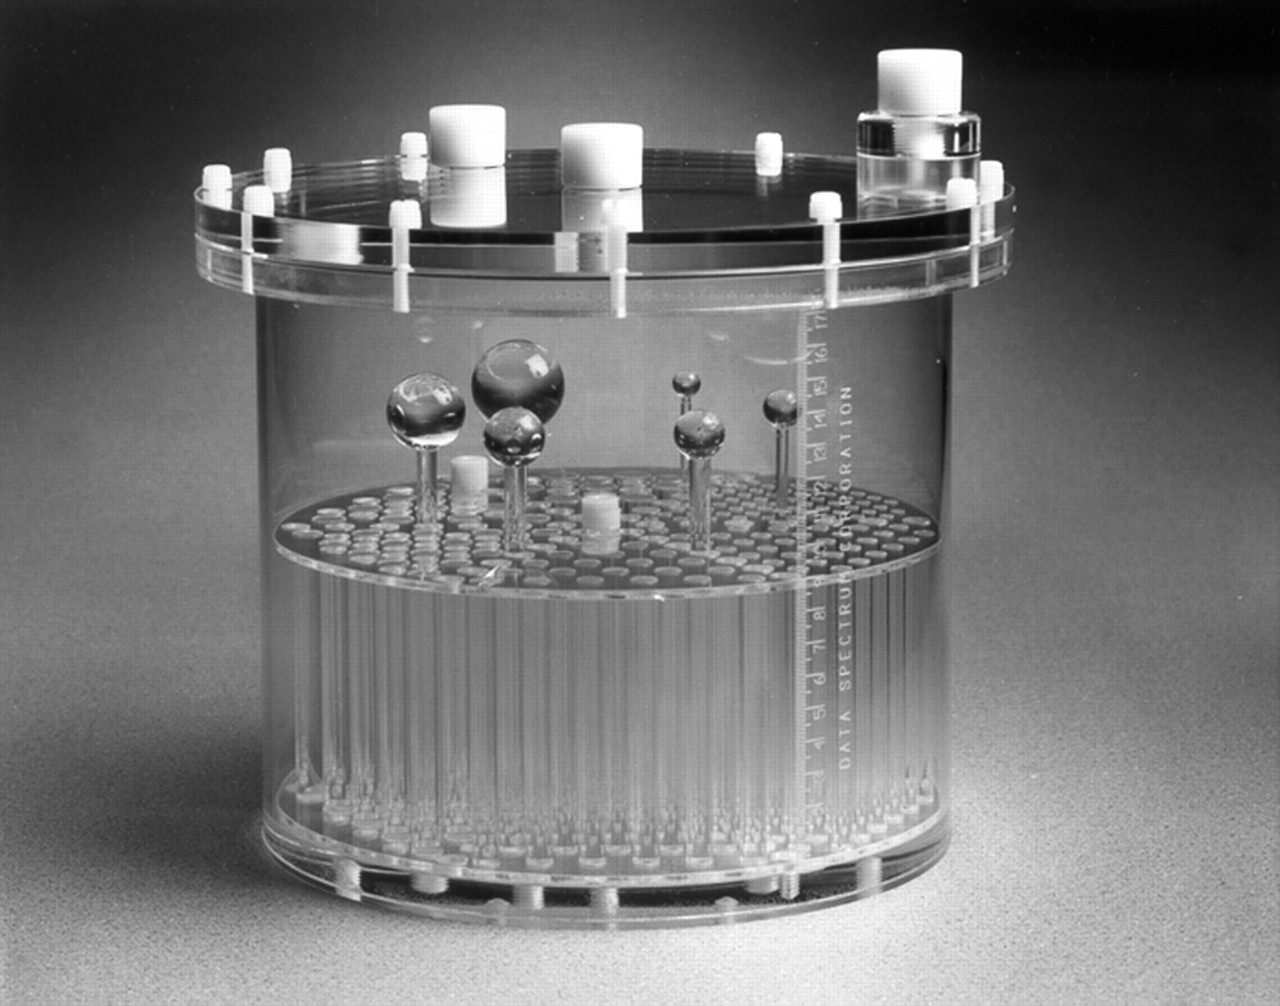
\includegraphics[width=\linewidth]{figures/Jaszczak}
	\end{figure}
\end{minipage}
\hfill
\begin{minipage}[c]{0.499\linewidth}
    \begin{figure}[H]
	\centering
	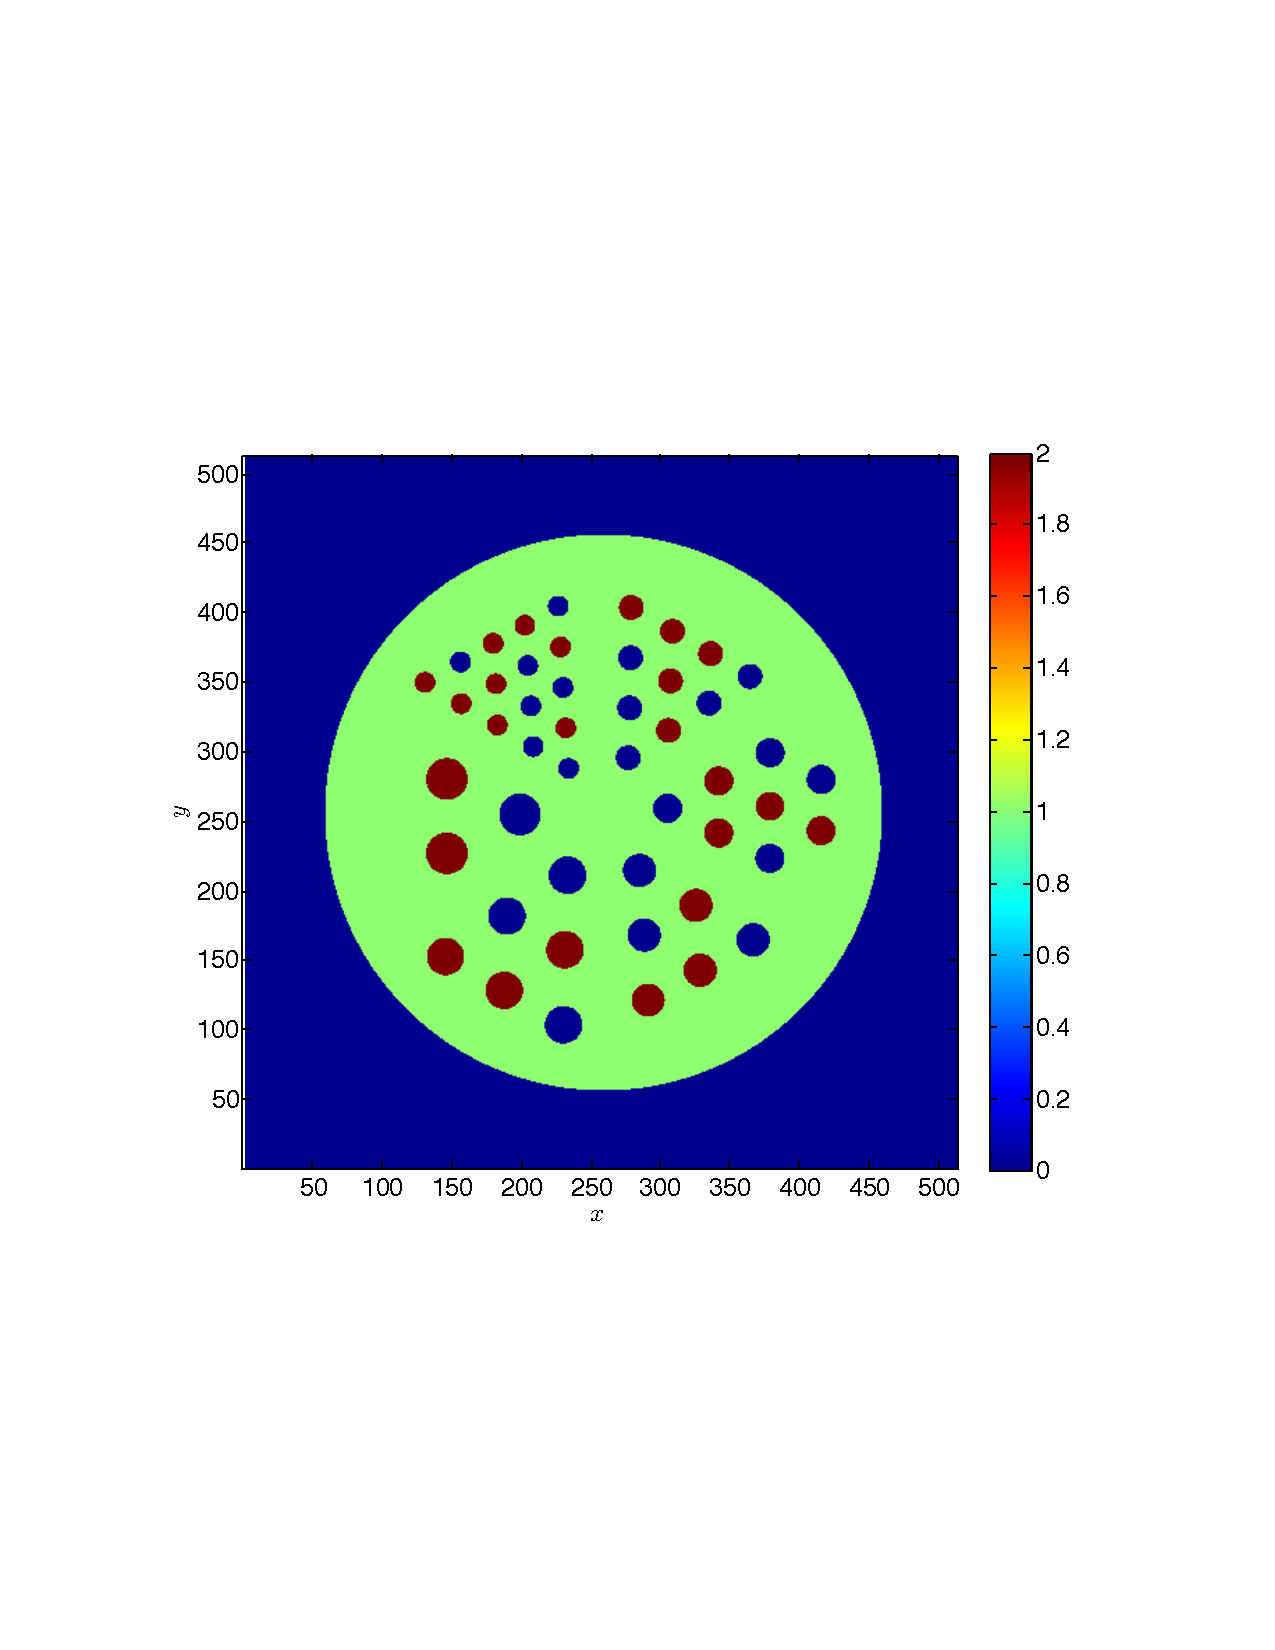
\includegraphics[width=.95\linewidth]{figures/JaszczakPhantom}
\end{figure}
\end{minipage}
	\caption[]{\emph{Left: the Jaszczak phantom device used for PET-scanner testing and calibration. A tracer liquid or inert water can be injected in each cylinder or sphere,  and in the phantom's main cylinder ( =  background).\\ \\
	Right ($\rightarrow$ \ref{fig:a1})\footnotemark: The true 2D image of the Jaszczak phantom that will be used in this chapter. Remark the uniform background of the cylinder in green (activity = 1), the hot regions in red (activity = 2) and the cold regions in blue (activity = 0).}}
	\label{fig:jaszczak}
\end{figure}

\footnotetext{Some images in this chapter have been included in a larger format in appendix A.}

This quantitative comparison of the MLEM and ISRA algorithms with realistic data obtained from analytic simulations will try to compare both algorithms based on the rate of convergence, the speed of reconstruction, and the bias and variance of the reconstructed image after a certain number of iterations. 




\section{Rate of convergence}
\setlength\intextsep{0pt}
\begin{wrapfigure}{r}{0.4\textwidth}
	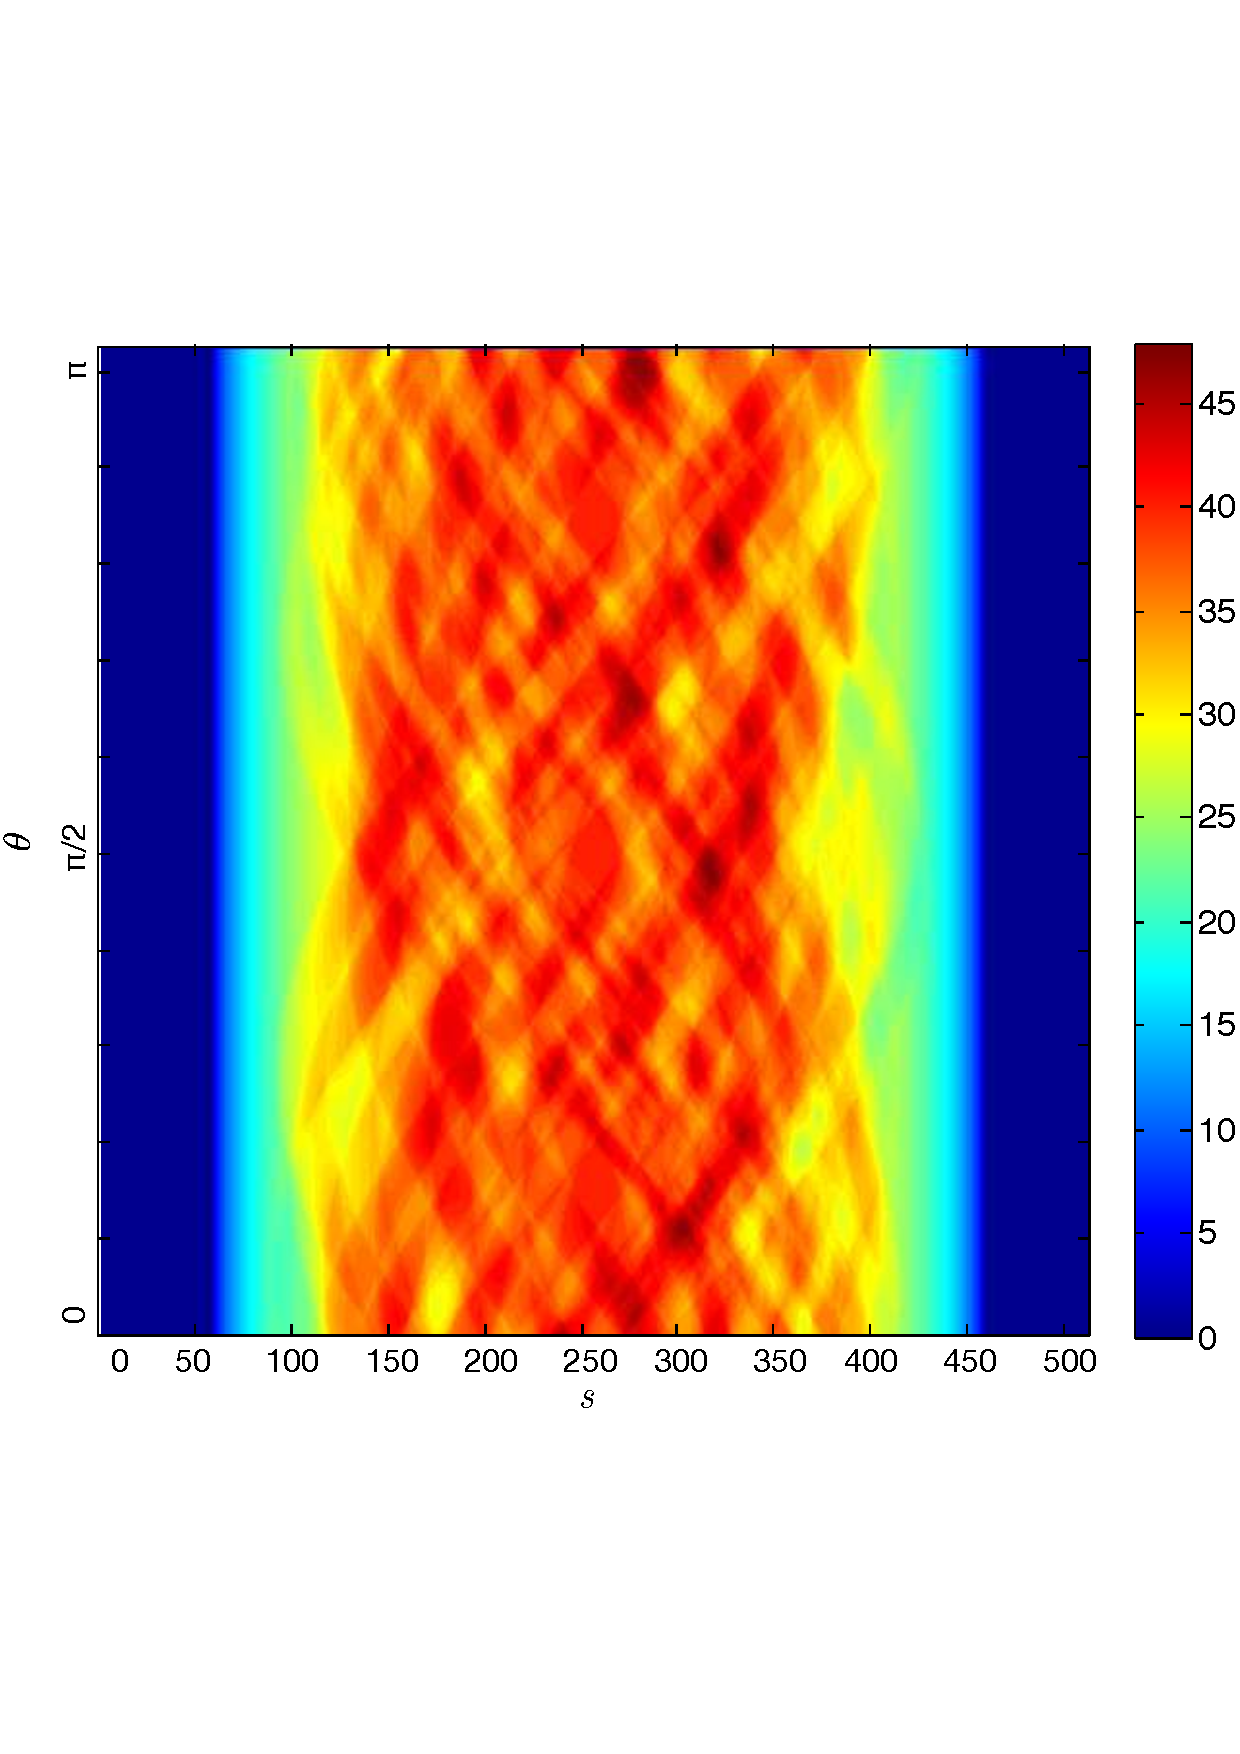
\includegraphics[width=\linewidth]{figures/sinogram}
	\caption{\emph{($\rightarrow$ \ref{fig:a2}): The noiseless sinogram of the Jaszczak phantom.}}
	\label{fig:sinogram}
\end{wrapfigure}
\intextsep\skip32
The first property of interest is the rate of convergence of the algorithms. Both MLEM and ISRA are known to converge to the exact image if the data is noiseless and if the likelihood is strictly concave. To study the rate of convergence as a function of the number of iterations, the image will be reconstructed from noiseless data and an objective criterium to quantify the rate of convergence will be introduced.\\ 
\hfill\\


The noiseless data is represented as a sinogram in figure \ref{fig:sinogram}. The sinogram has 512 radial pixels and 512 views from $\uptheta$ = 0 to $\uppi$. The images reconstructed with MLEM and ISRA are in figures  \ref{fig:NoiselessReconstructionMLEM} and \ref{fig:NoiselessReconstructionISRA}. These figures are normalised in the sense that for each iteration, the minimum and maximum of the colour maps have the same values. This allows quick visual comparison between MLEM and ISRA.
\intextsep\savedintextsep
\begin{figure}[H]
	\begin{minipage}[t]{\textwidth}
		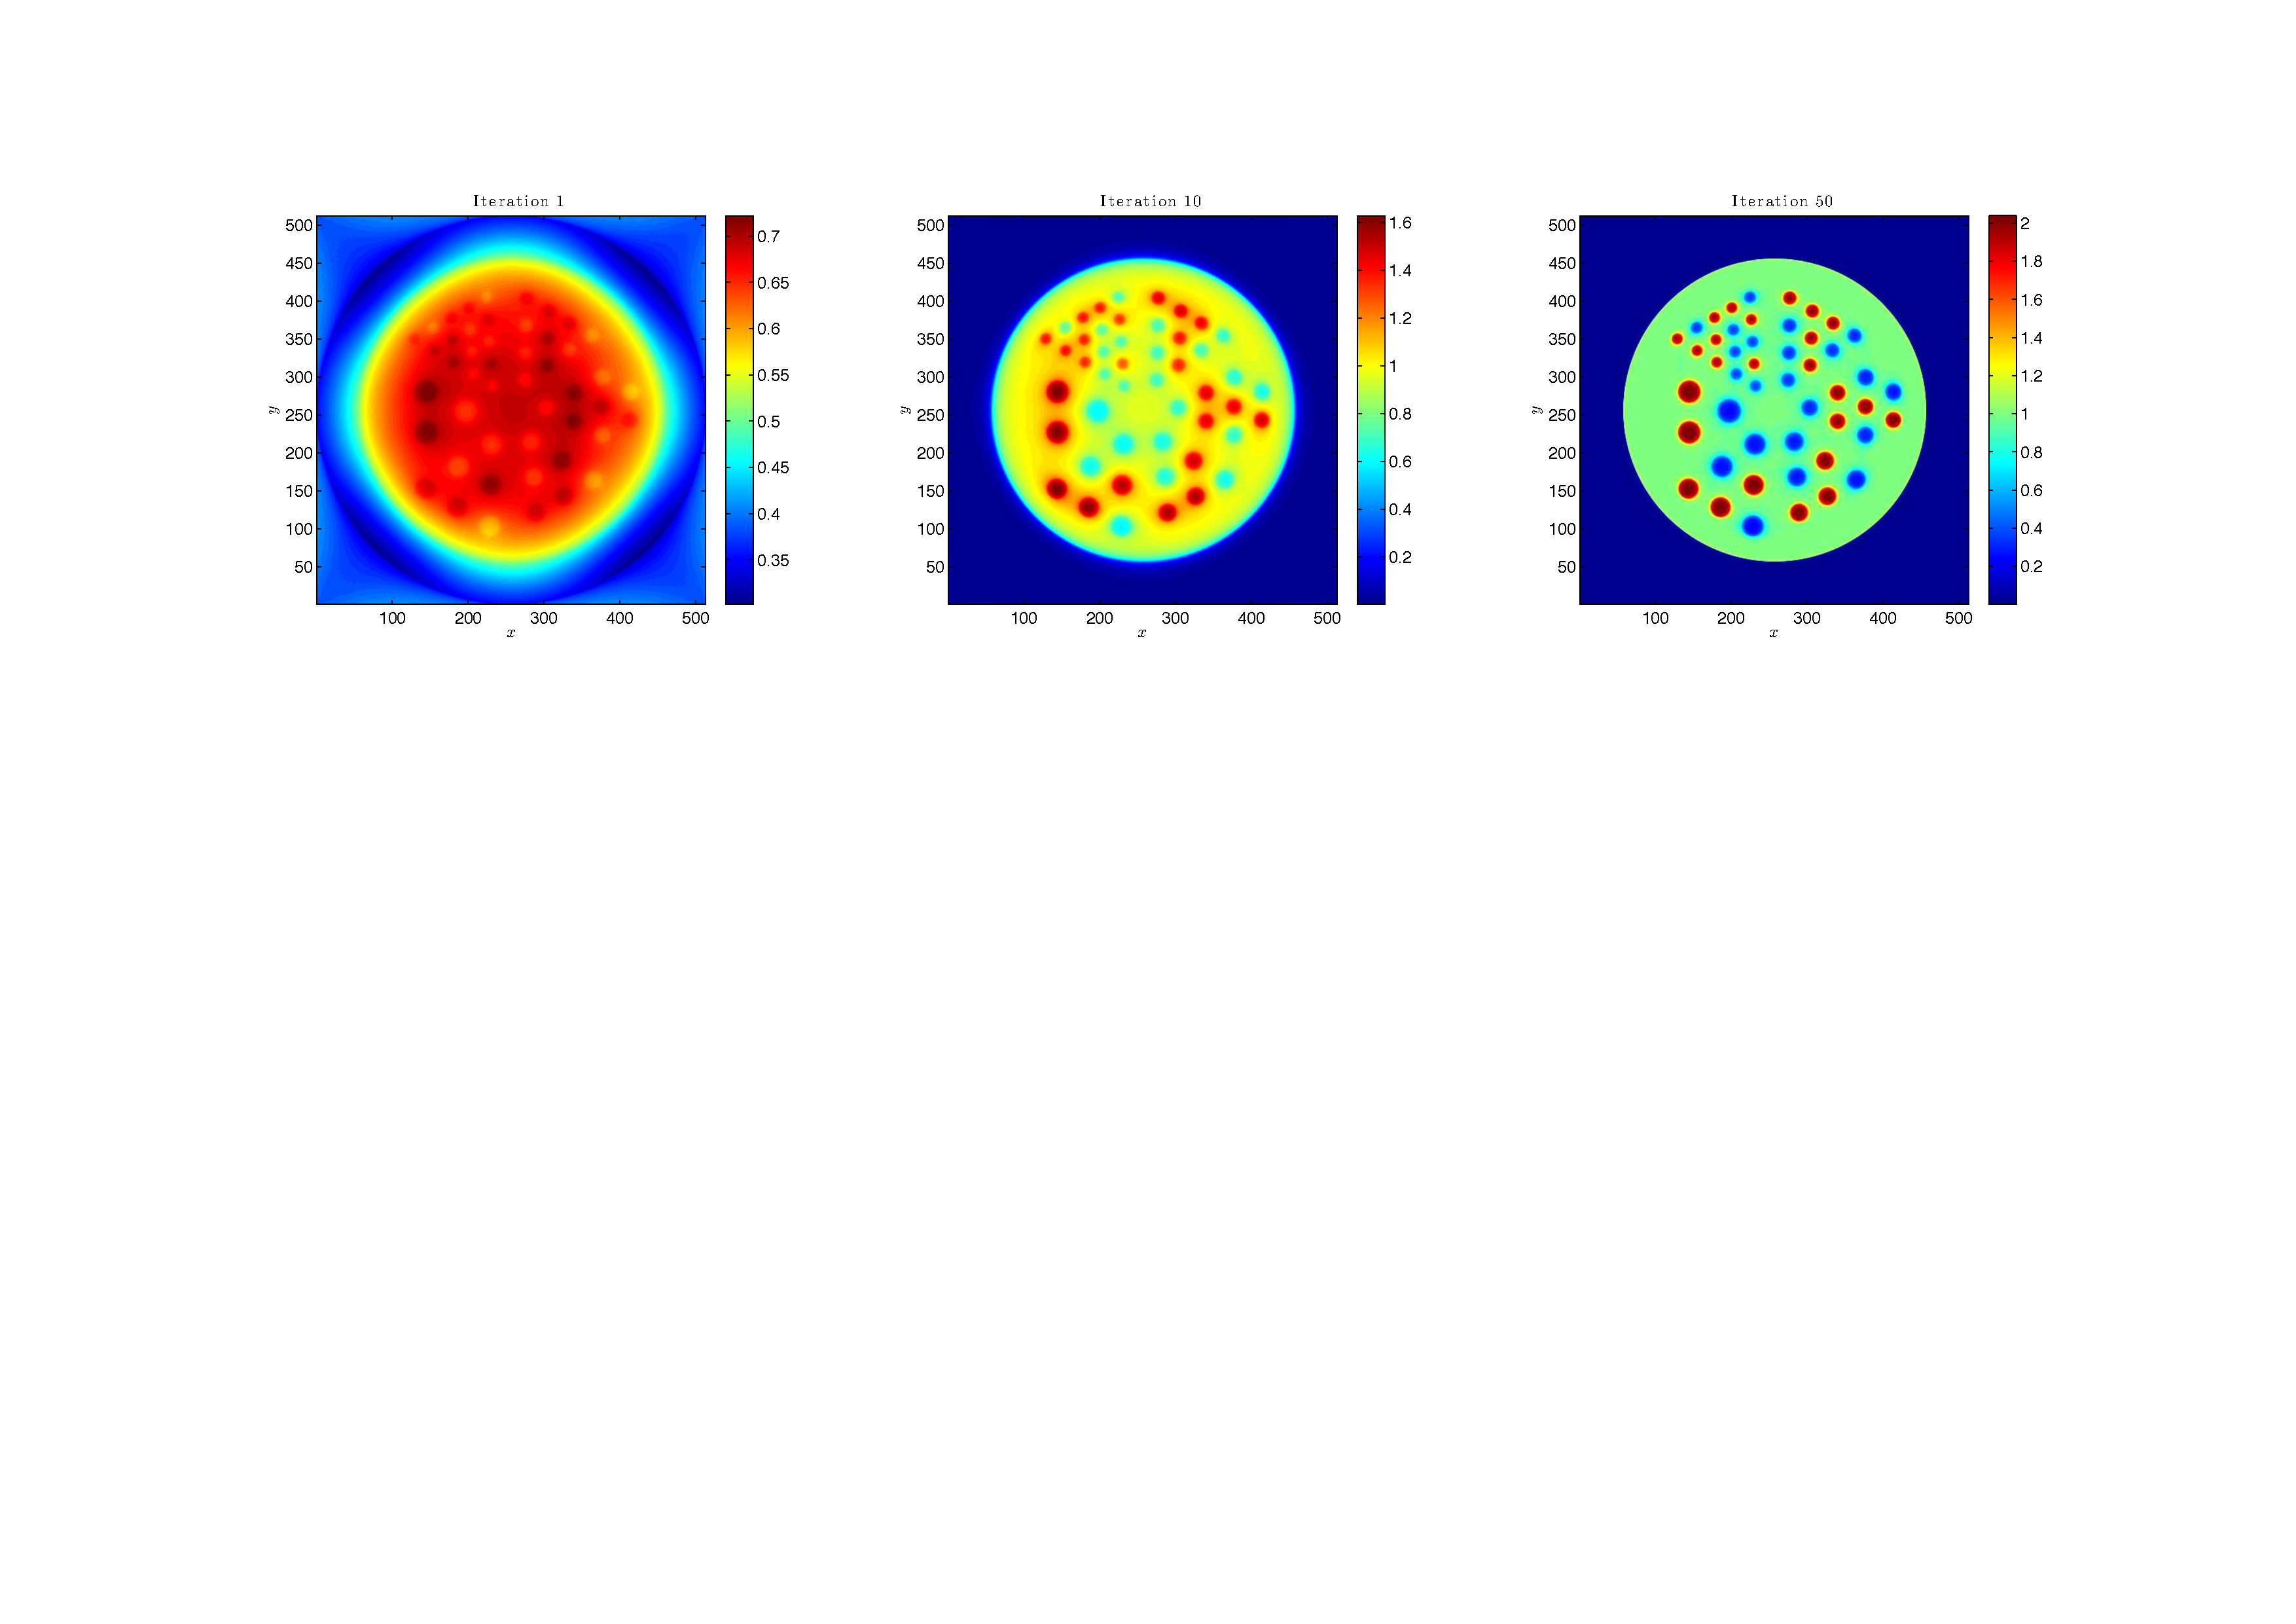
\includegraphics[width=\linewidth]{figures/MLEMNoiselessConvergence1}
  	\end{minipage}\hfill
  	\begin{minipage}[t]{\textwidth}
		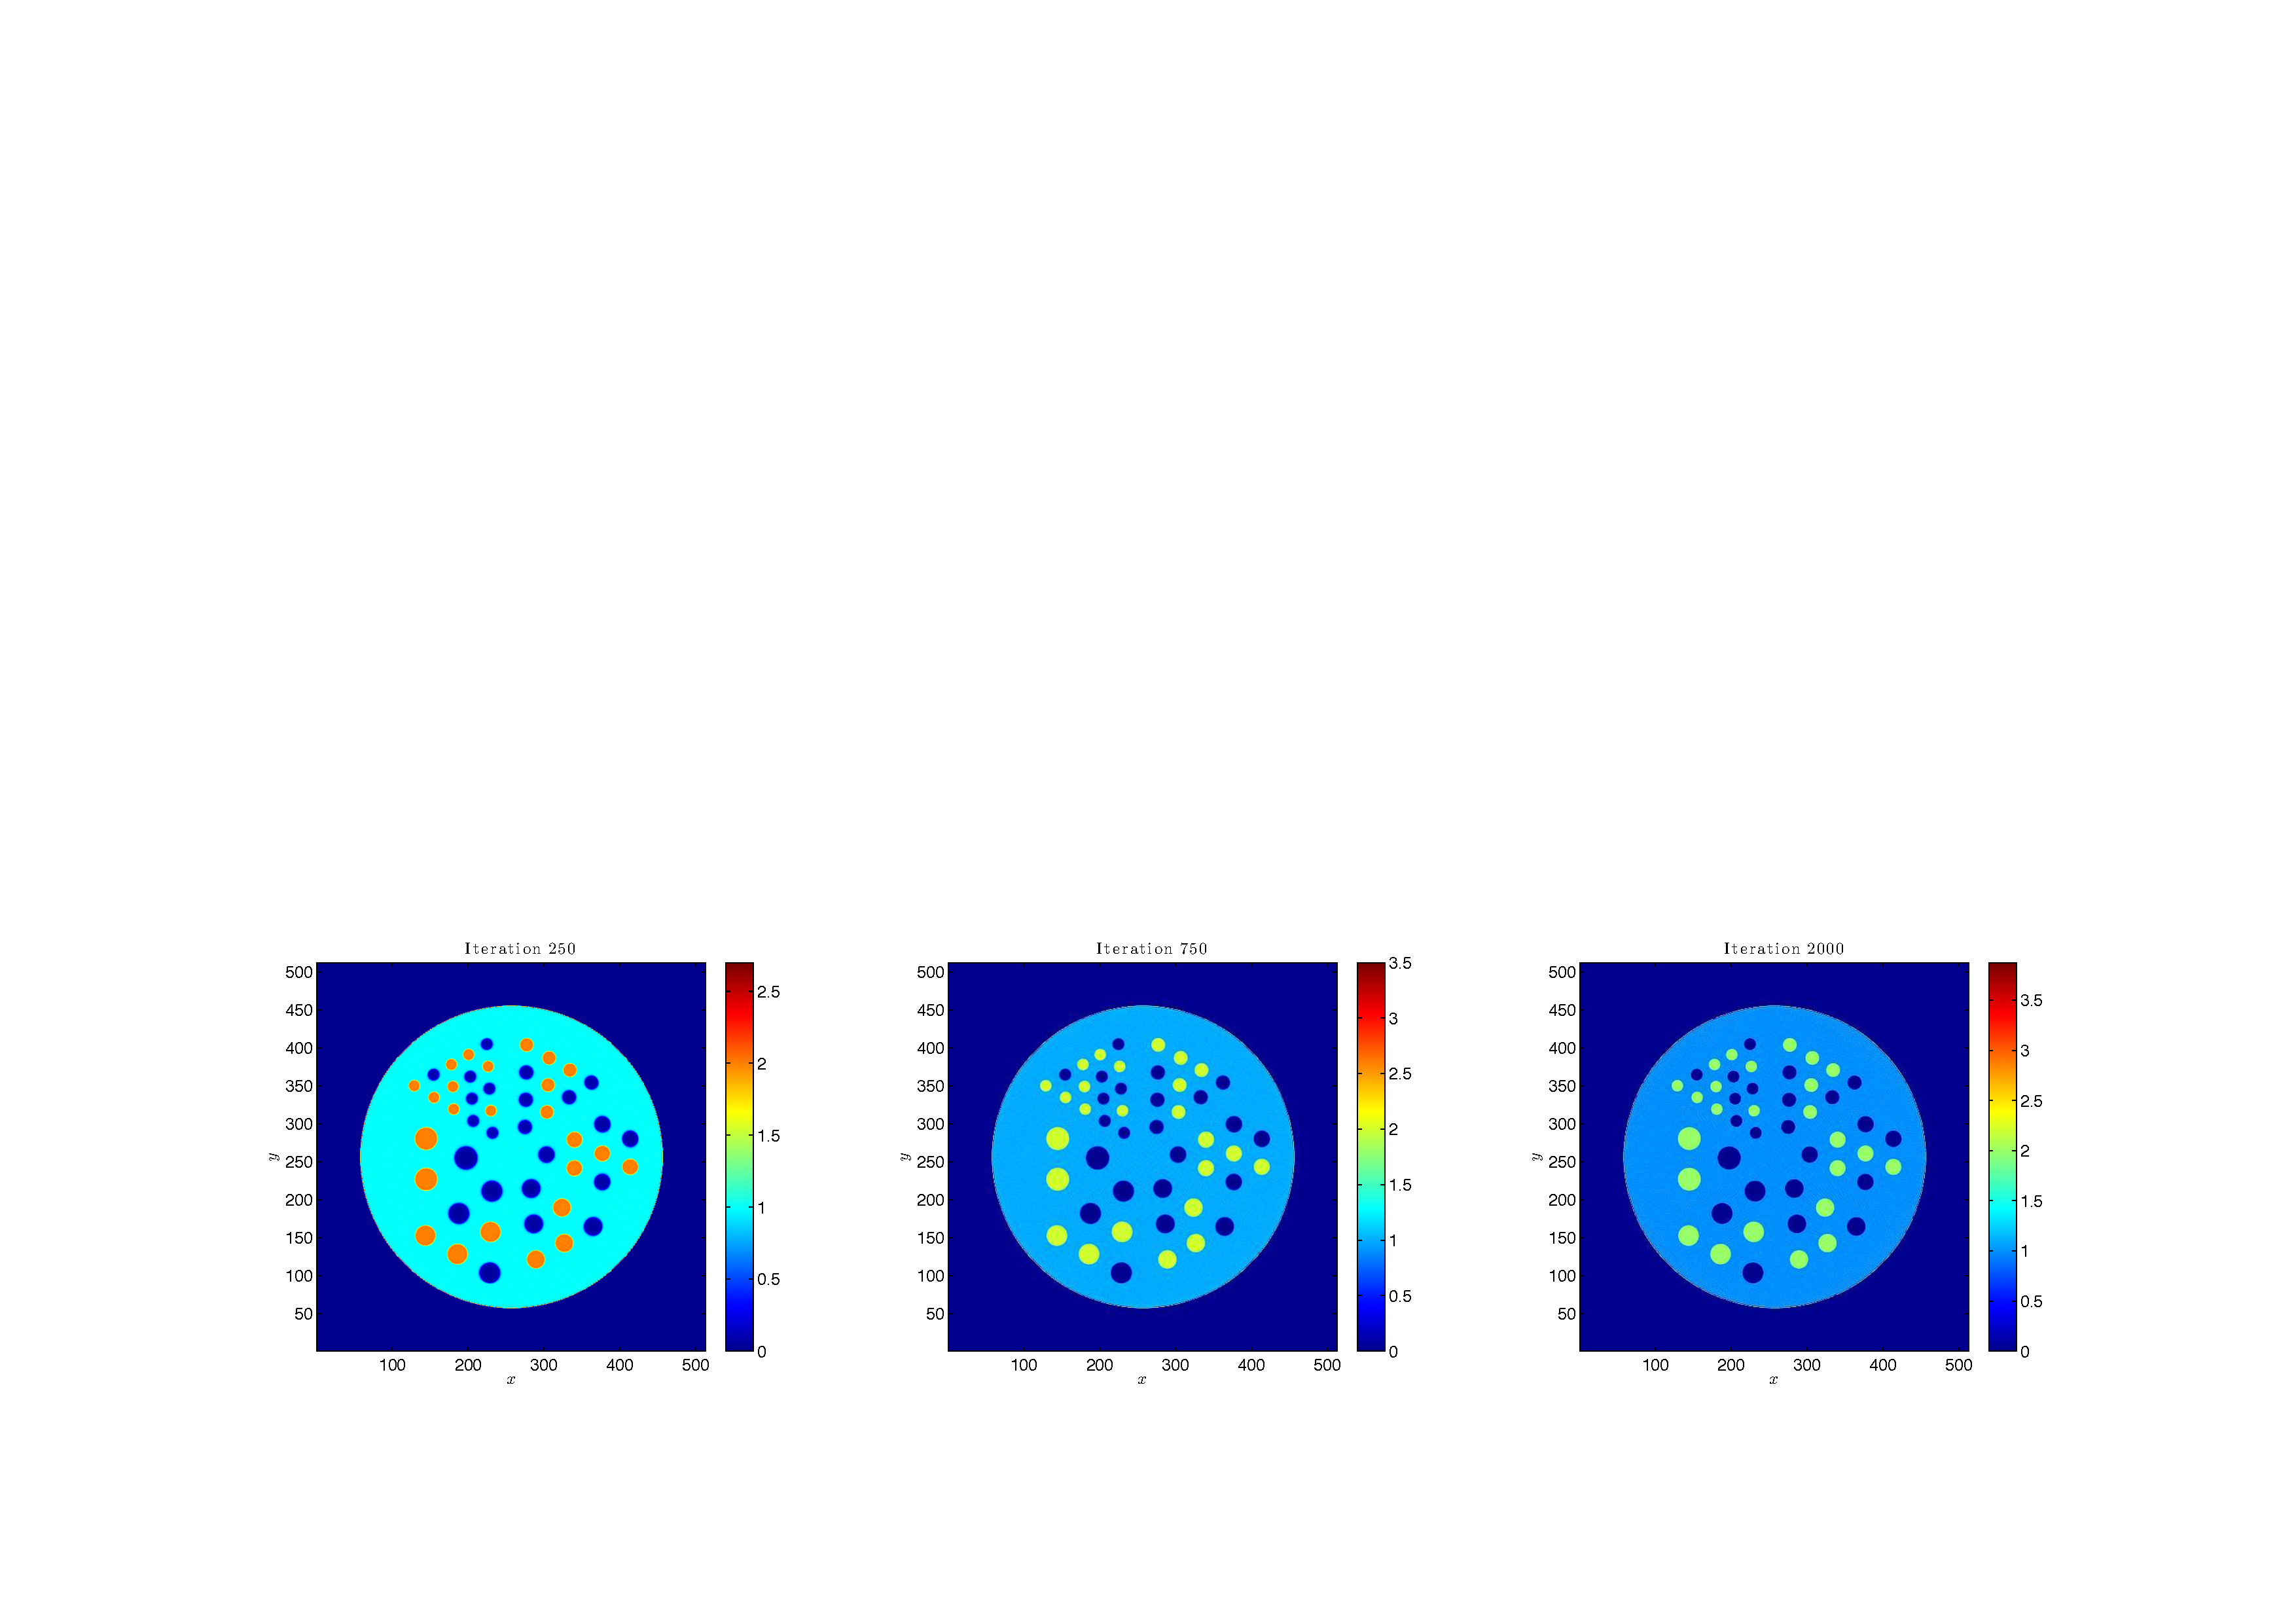
\includegraphics[width=\linewidth]{figures/MLEMNoiselessConvergence2}
  	\end{minipage}
	\caption{\emph{($\rightarrow$ \ref{fig:a3}): The iterative image reconstruction of the Jaszczak phantom with MLEM starting from the exact sinogram in figure \ref{fig:sinogram}.}}
	\label{fig:NoiselessReconstructionMLEM}
\end{figure}
\intextsep\savedintextsep
\begin{figure}[H]
	\begin{minipage}[t]{\textwidth}
		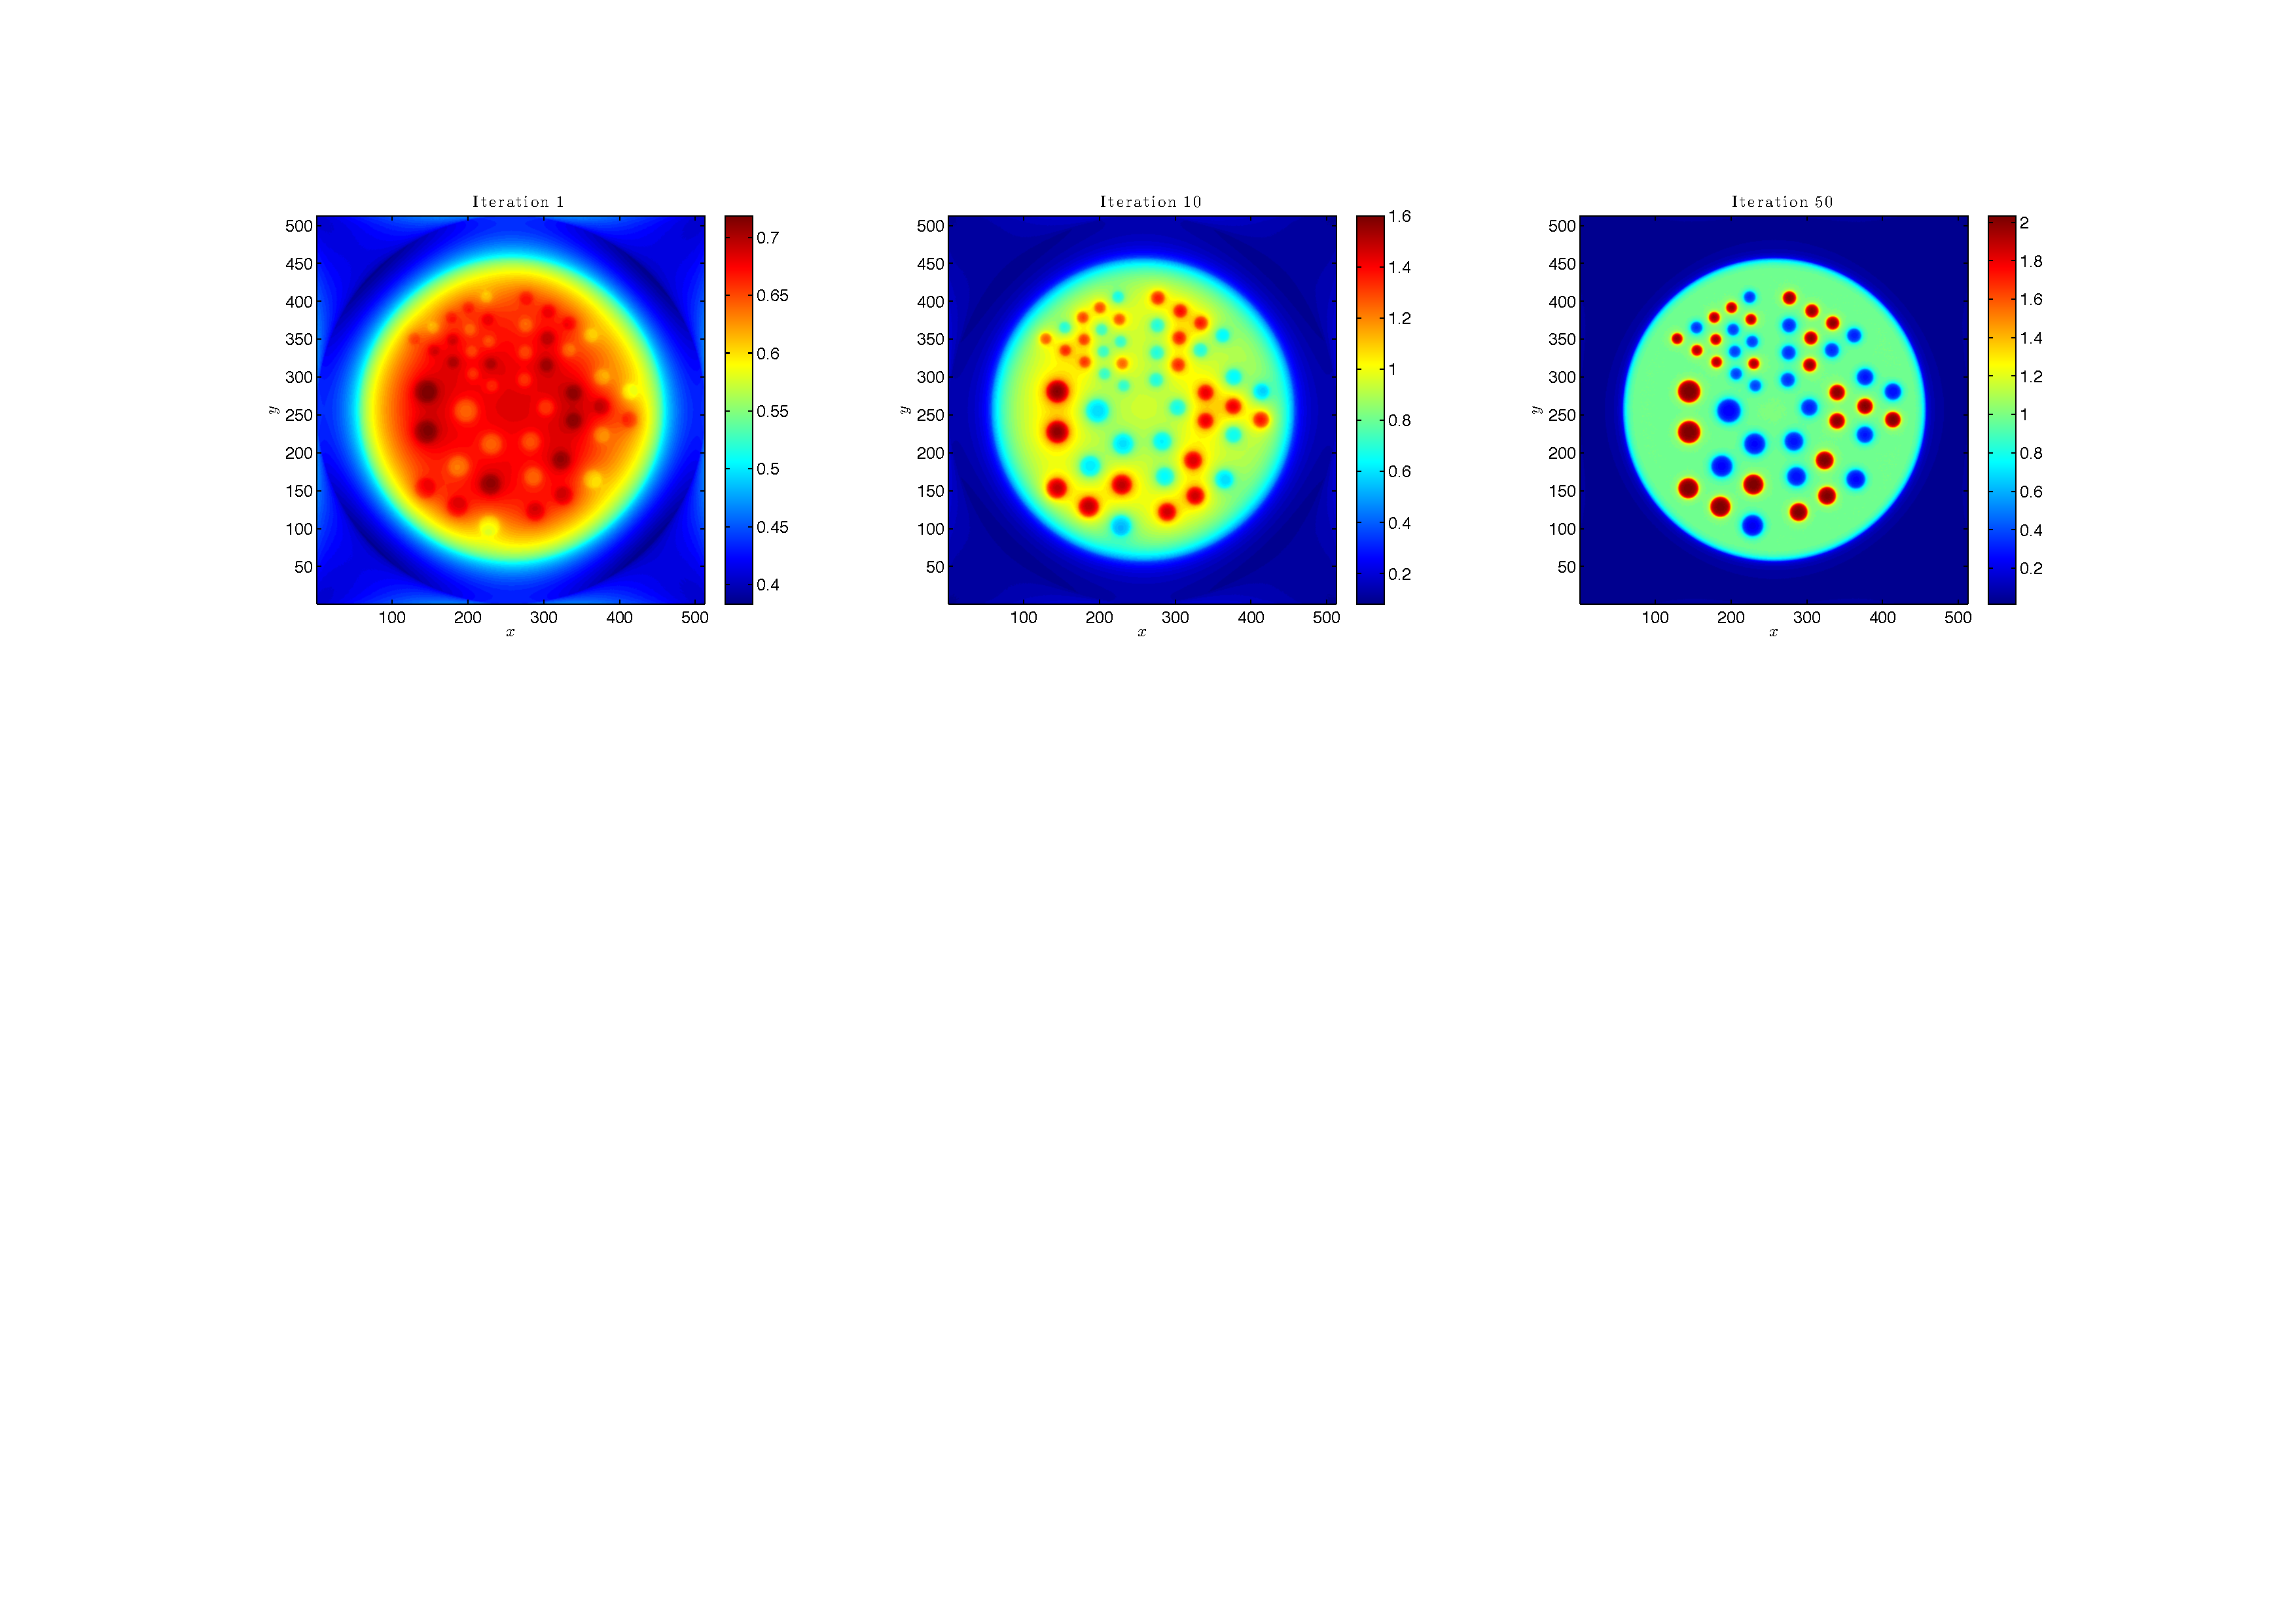
\includegraphics[width=\linewidth]{figures/ISRANoiselessConvergence1}
  	\end{minipage}\hfill
  	\begin{minipage}[t]{\textwidth}
		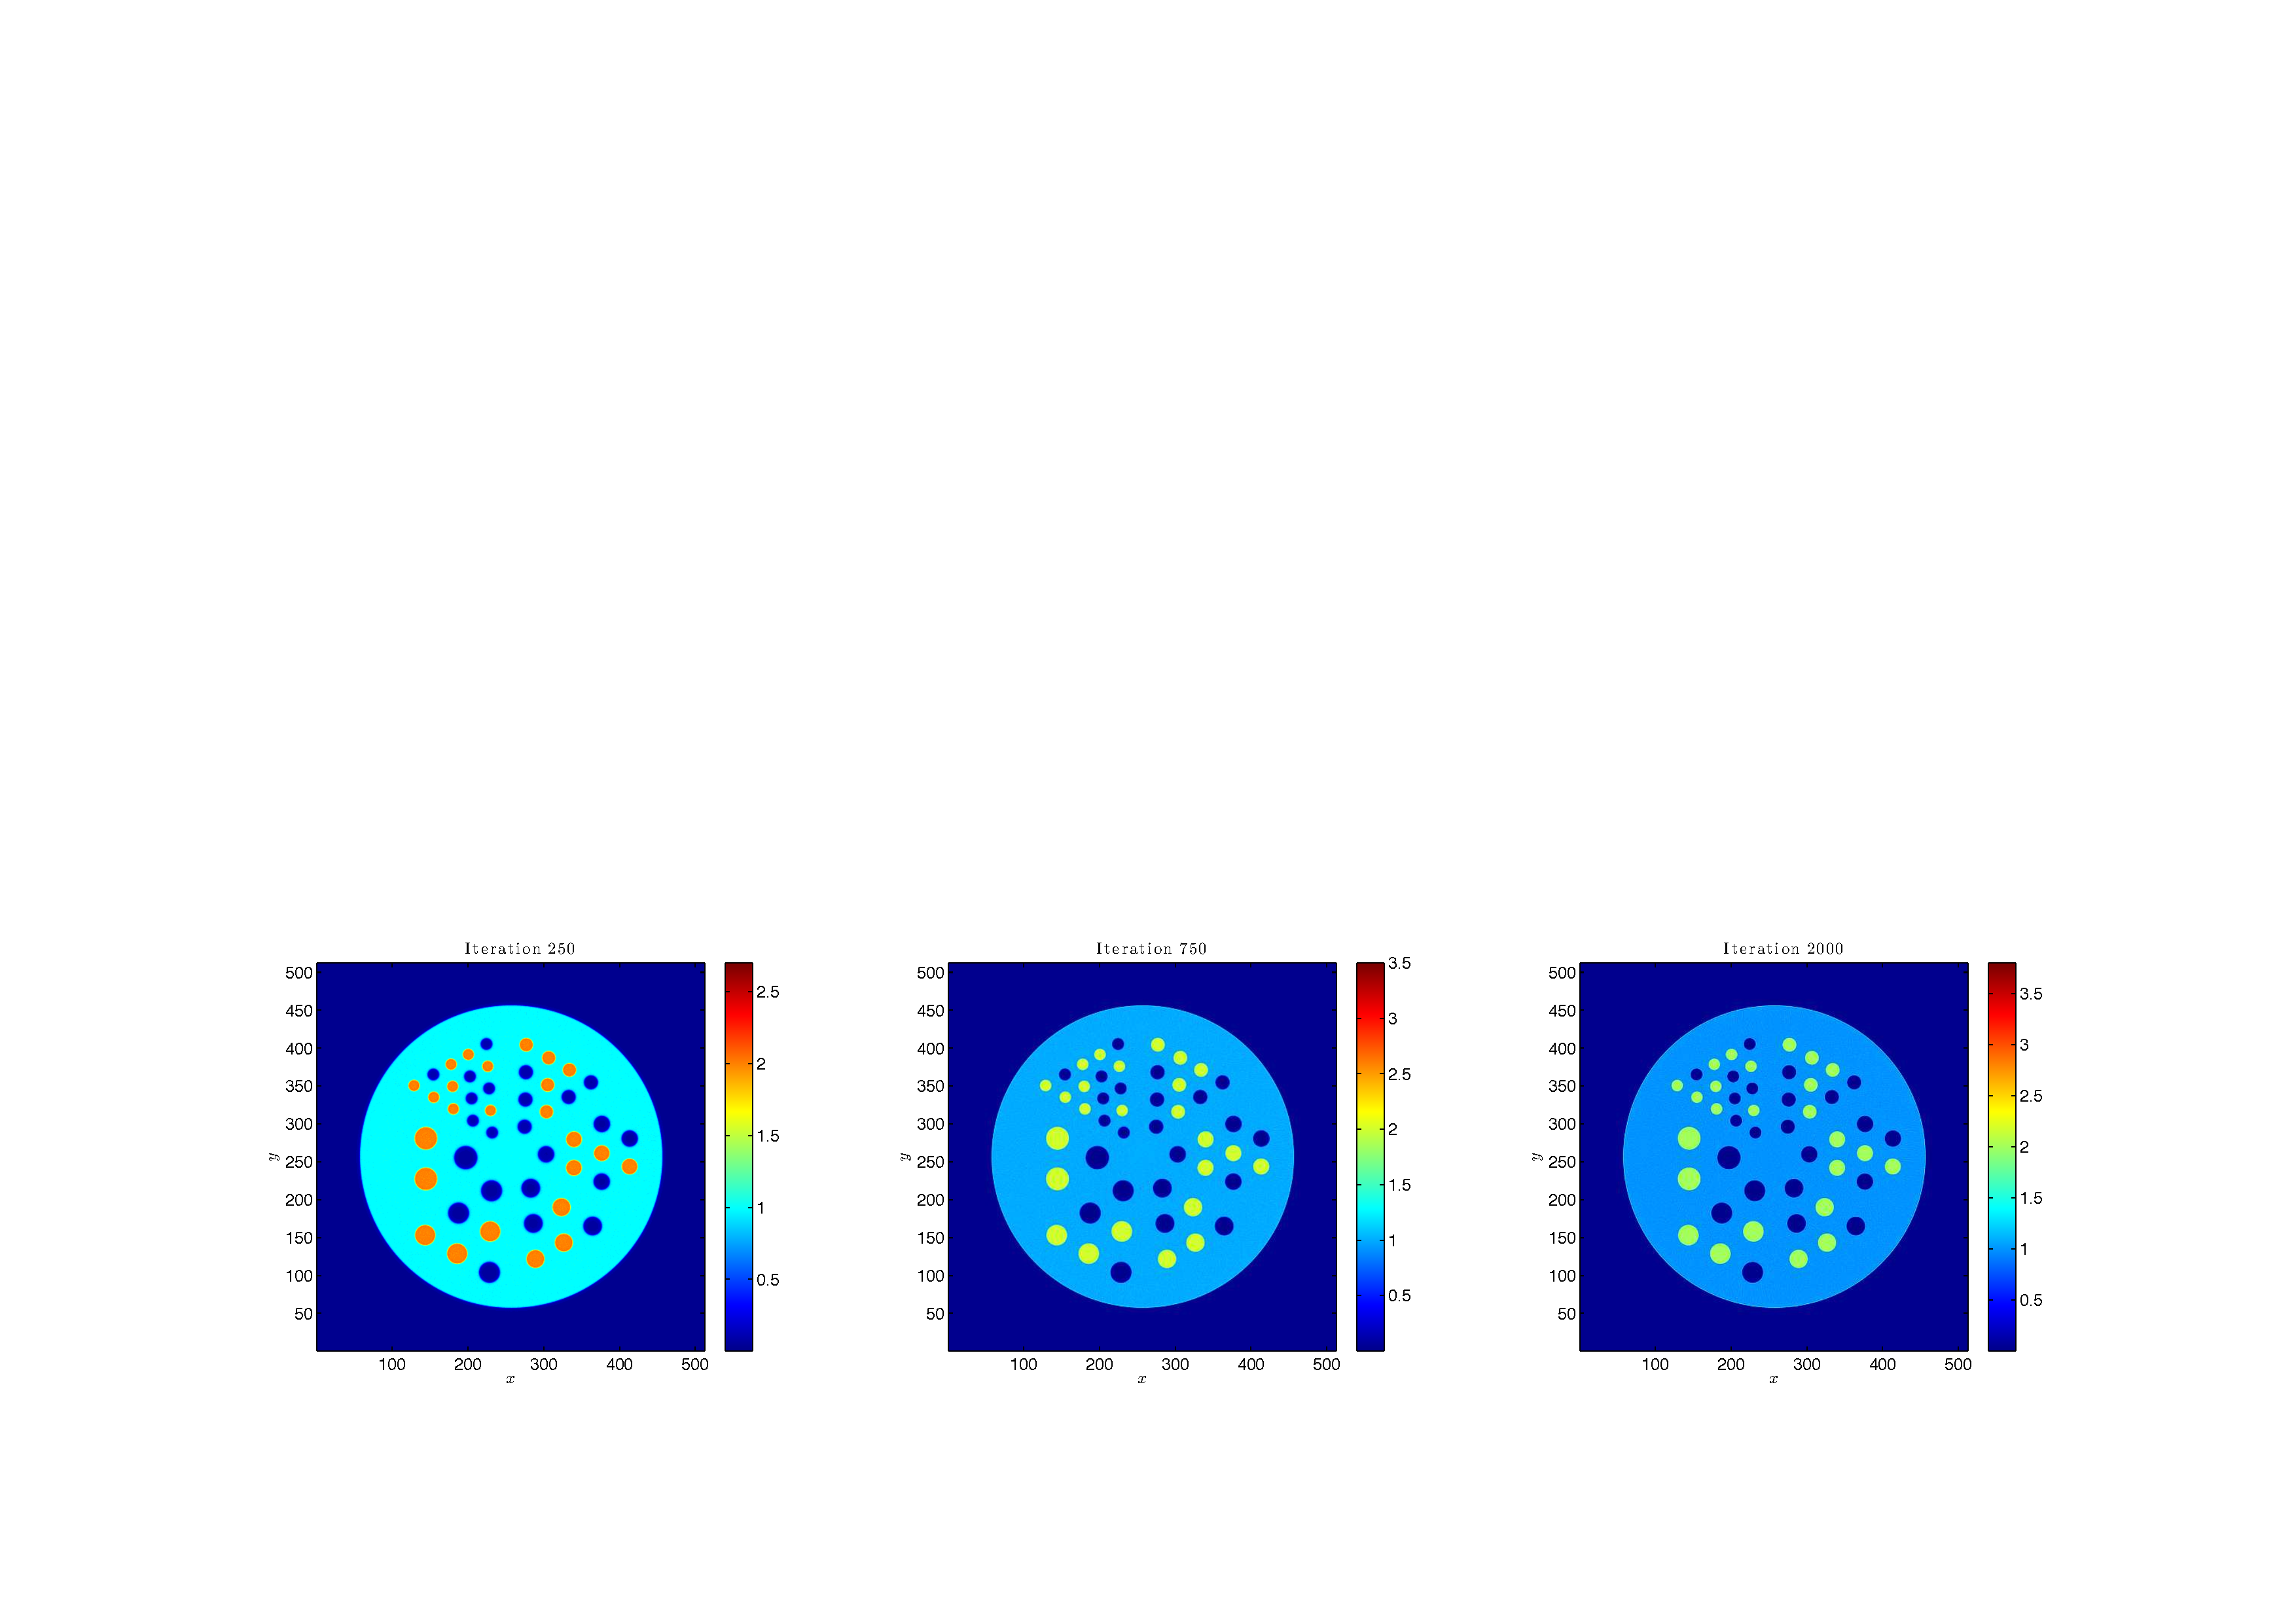
\includegraphics[width=\linewidth]{figures/ISRANoiselessConvergence2}
  	\end{minipage}
	\caption{\emph{($\rightarrow$ \ref{fig:a4}): The iterative image reconstruction of the Jaszczak phantom with ISRA starting from the exact sinogram in figure \ref{fig:sinogram}.}}
	\label{fig:NoiselessReconstructionISRA}
\end{figure}




Visually it looks like the convergence of MLEM and ISRA is similar and reaches comparable image qualities in about the same number of iterations. This statement can be quantified by measuring the difference in total value of the image at iteration $n$ and iteration $n+1$. Once the algorithm has converged, the difference between iteration $n$ and iteration $n+1$ is 0. So a criterium for convergence could be 
\begin{align}
	\Delta(I_n, I_{n+1}) = \sum_i \mid p_x(i,n) - p_x(i,n+1) \mid< \varepsilon,\ \ \ \ \  \varepsilon > 0\footnotemark
\end{align}
\footnotetext{Theoretically $\varepsilon$ can become arbitrarily small depending on how close the algorithm is to convergence, though in practice the computer's finite precision must be considered.}
where $I_{n(+1)}$ is the image at iteration $n(+1)$, $\Delta$ measures the total difference between two images, the summation is over all pixels of the image, and $p_x(i,n(+1))$ is the value of pixel $i$ at iteration $n(+1)$. The absolute value ensures that if from one iteration to the next some pixels decrease in value and others increase in value, the differences do not compensate.\\

The evolution of $\Delta$ is plotted for MLEM and ISRA in figure \ref{fig:RateOfConvergence}. The convergence rate of both algorithms is quite comparable. For the 400 first iterations MLEM converges a bit more rapidly, but afterwards ISRA is a bit faster.\\

It is also possible to make a $\Delta$-image to see which regions of the image undergo the biggest changes. For MLEM and ISRA at iteration 1999 and 2000, the $\Delta$-images are in figure \ref{fig:AlgorithmConvergenceTest} with $\Delta_{MLEM} = 2.43$ and $\Delta_{ISRA} = 1.48$. The difference are more pronounced on the borders between hot and cold regions. The largest differences do not exceed 0.000278 for MLEM and 0.000147 for ISRA.\\

These results show that MLEM and ISRA reach a certain quality of reconstruction in a number of iterations that is in the same order of magnitude. 
\setlength\intextsep{\savedintextsep}
\begin{figure}[H]
	\centering
	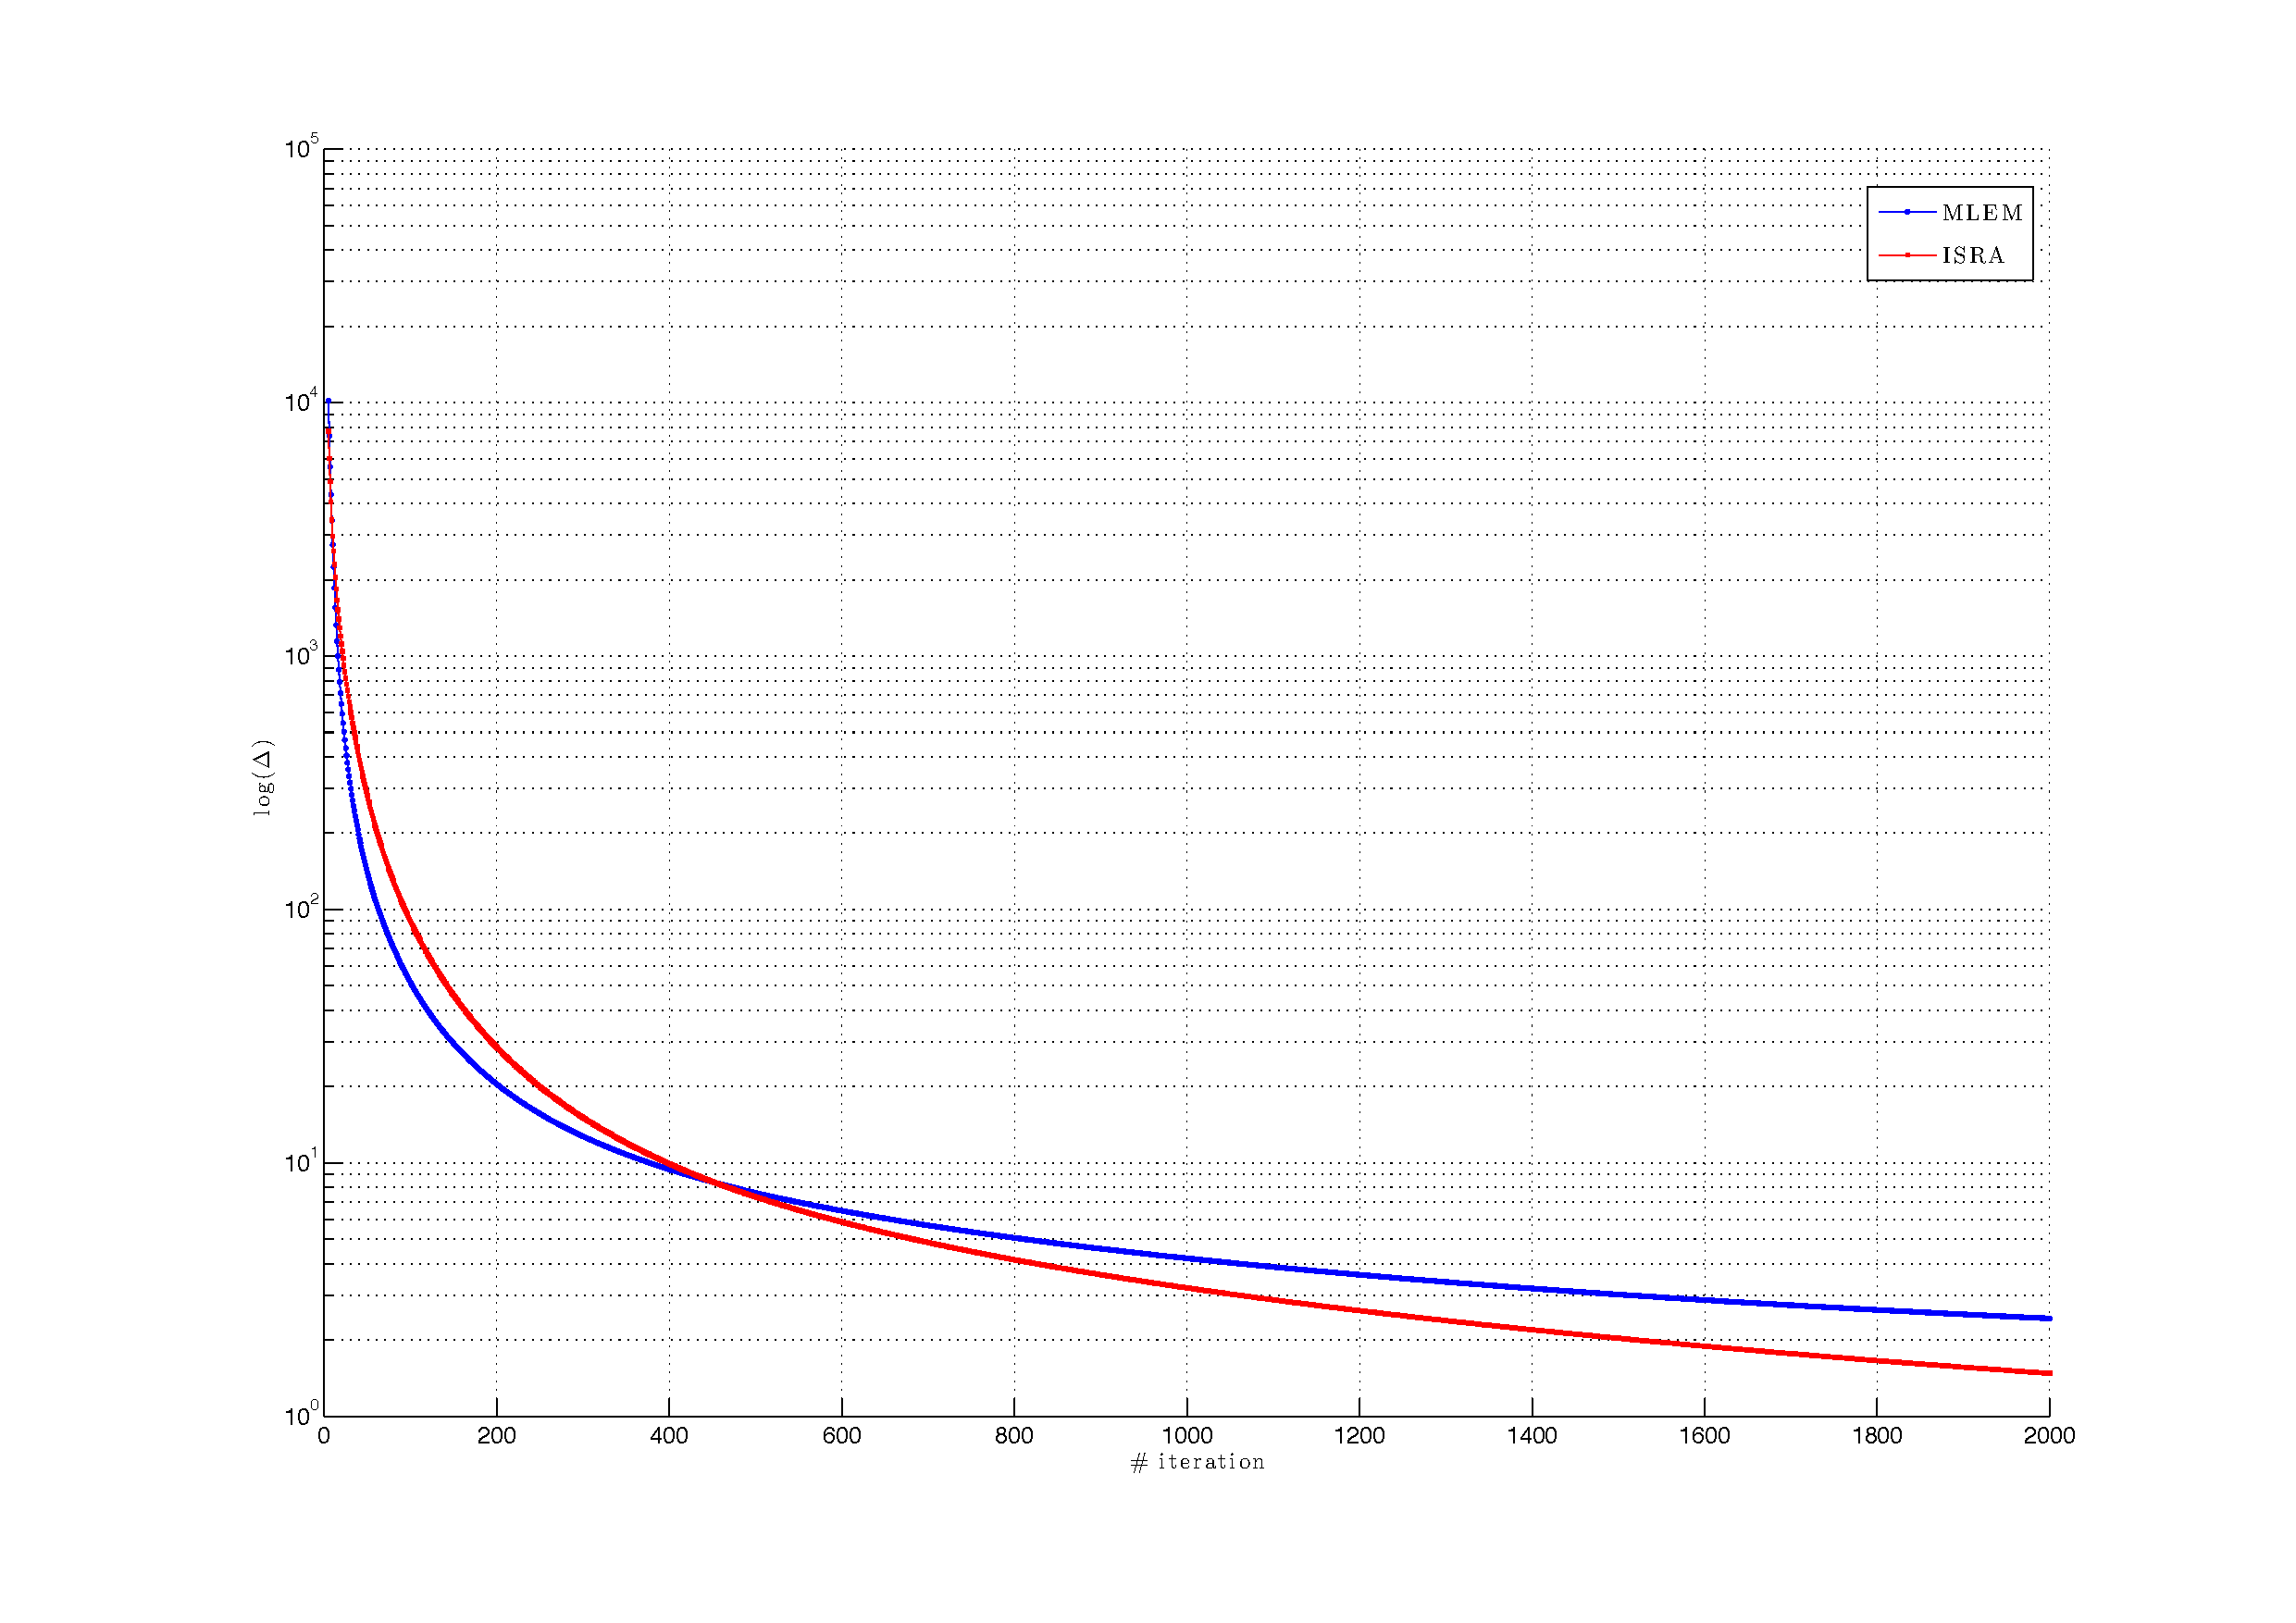
\includegraphics[width=.65\linewidth]{figures/RateOfConvergence.pdf}
	\caption{\emph{($\rightarrow$ \ref{fig:a45}): The rate of convergence for MLEM (blue) and ISRA (red).}}
	\label{fig:RateOfConvergence}
\end{figure}

\setlength\intextsep{\savedintextsep}
\begin{figure}[H]
\centering
	\begin{minipage}[t]{0.5\textwidth}
	\centering
		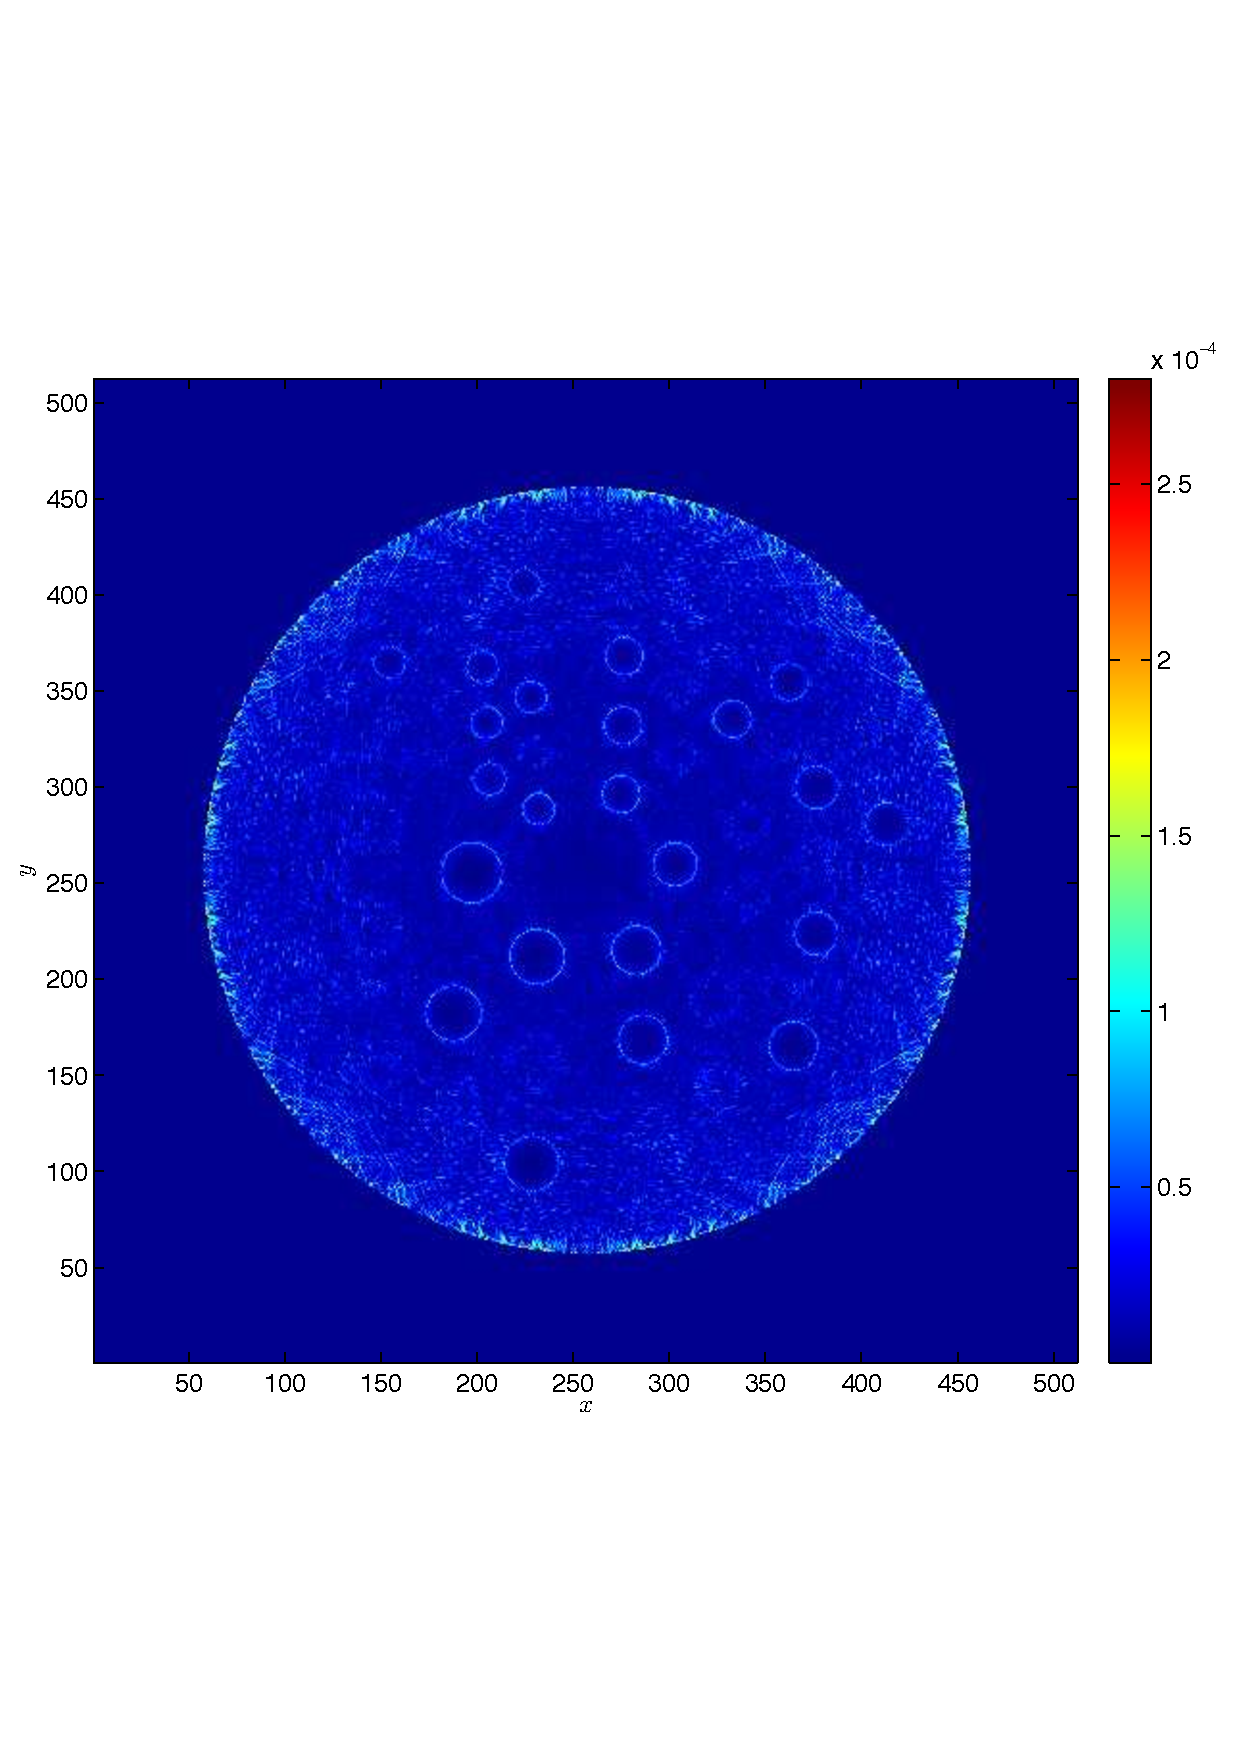
\includegraphics[width=0.8\linewidth]{figures/osemDelta6}
  	\end{minipage}\hfill
  	\begin{minipage}[t]{0.5\textwidth}
	\centering
		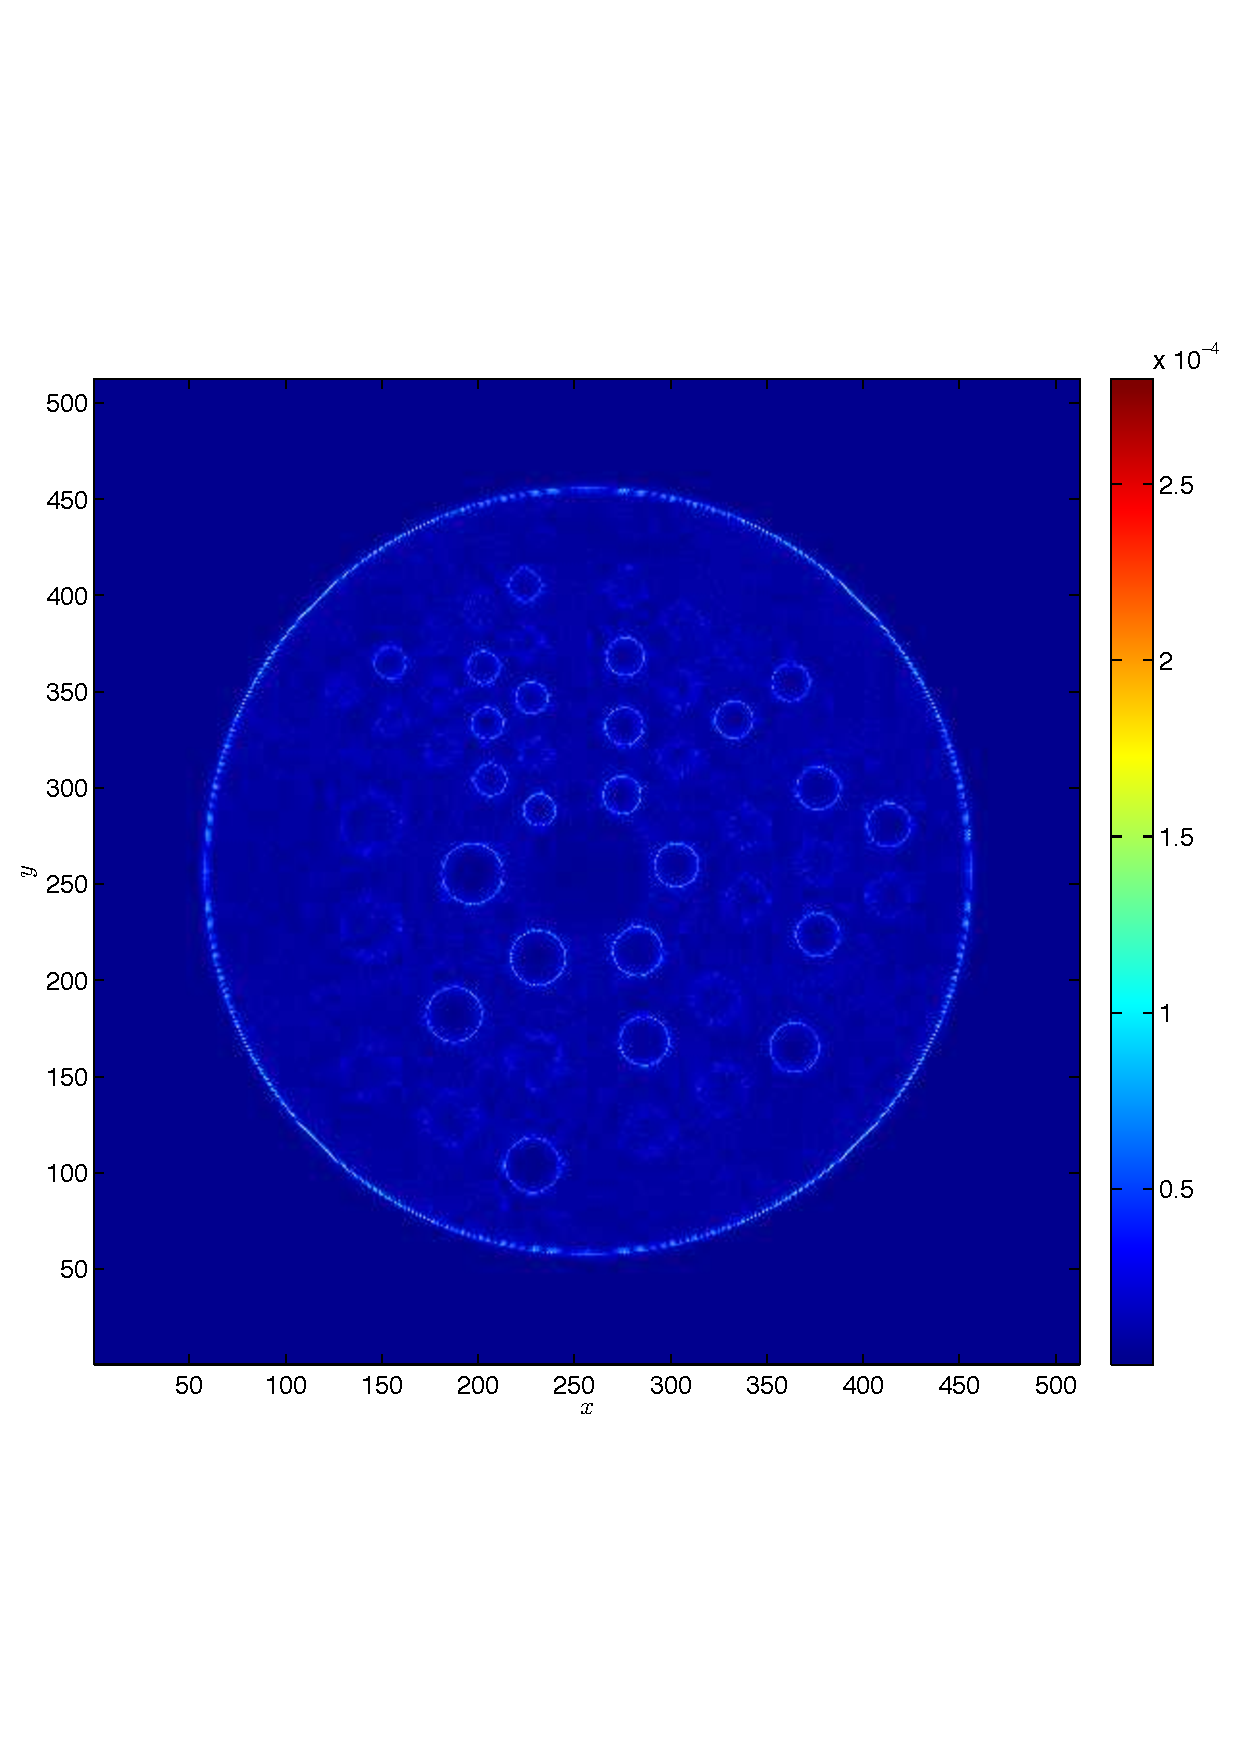
\includegraphics[width=0.8\linewidth]{figures/israDelta6}
  	\end{minipage}
	\caption{\emph{($\rightarrow$ \ref{fig:a5}): The difference between iteration 1999 and 2000 for MLEM (left) and ISRA (right).}}
	\label{fig:AlgorithmConvergenceTest}
\end{figure}




\section{Speed of reconstruction}
Not only the number of iterations after which a certain quality of reconstruction is achieved is important, but the computational time required to perform one iteration is important as well. The computational time required depends on the available hardware, but the results below allow to compare both algorithms qualitatively if not quantitatively.
\setlength\intextsep{\savedintextsep}
\begin{table}[H]
\centering
\begin{tabular}{lllllll}
\cline{1-3} \cline{5-7}
\multicolumn{3}{|l|}{\begin{tabular}[c]{@{}l@{}}2.2 GHz Intel dual-core i5\\ Number of iterations: 100\end{tabular}} & \multicolumn{1}{l|}{\multirow{3}{*}{}} & \multicolumn{3}{l|}{\begin{tabular}[c]{@{}l@{}}2.8 GHz Intel quad-core i7\\ Number of iterations: 250\end{tabular}} \\ \cline{1-3} \cline{5-7} 
\multicolumn{3}{l}{}                                                                                                              & \multicolumn{1}{l|}{}                  & \multicolumn{3}{l}{}                                                                                                             \\ \cline{1-3} \cline{5-7} 
\multicolumn{1}{|l|}{MLEM}        & \multicolumn{1}{l|}{239 s}        & \multicolumn{1}{l|}{2.39 s / iteration}        & \multicolumn{1}{l|}{}                  & \multicolumn{1}{l|}{MLEM}        & \multicolumn{1}{l|}{326 s}        & \multicolumn{1}{l|}{1.30 s / iteration}        \\ \cline{1-3} \cline{5-7} 
\multicolumn{1}{|l|}{ISRA}        & \multicolumn{1}{l|}{170 s}        & \multicolumn{1}{l|}{1.70 s / iteration}        & \multicolumn{1}{l|}{}                  & \multicolumn{1}{l|}{ISRA}        & \multicolumn{1}{l|}{311 s}        & \multicolumn{1}{l|}{1.24 s / iteration}        \\ \cline{1-3} \cline{5-7} 
\end{tabular}
	\caption{\emph{Iteration time on different machines.}}
	\label{tab:ReconstructionSpeed}
\end{table}

This table shows that execution times depend on the specific hardware, but it also shows that MLEM and ISRA can be expected to iterate in times that are of the same order of magnitude. This similarity in time per iteration can be explained by comparing the algorithms' conceptual expressions. MLEM is conceptually (eq. \ref{eq:MLEMConceptually})
\begin{align}
	\hat{\vec{x}}^{next} = \hat{\vec{x}}^{current} \frac{Backproject\left( \frac{\vec{y}}{Project\left( \hat{\vec{x}}^{current} \right)} \right)}{Backproject\left(\vec 1\right)}
\end{align} 

Remark that the $Backproject(\vec 1)$ operation only has to be performed once, and not for each individual iteration.\\

ISRA is conceptually (eq. \ref{eq:ISRAConceptual})
\begin{align}
	\hat{\vec{x}}^{next} = \hat{\vec{x}}^{current} \frac{Backproject(\vec y)}{Backproject(\ Project(\hat{\vec{x}}^{current}))}
\end{align}

For ISRA the $Backproject(\vec y)$ operation only has to be performed once. Both algorithms can be decomposed and represented in pseudo-code.\\
\setlength\intextsep{\savedintextsep}
        	\begin{minipage}[t]{.499\linewidth}
        	\centering
        	\textbf{MLEM}
        		\begin{align}
        			&\mathbf{ \begingroup\color{red}1.\endgroup}\ Backproject(\vec 1)\rightarrow X\nonumber\\
        			&\mathbf{\begingroup\color{orange}2.\endgroup}\ for(iterations):\nonumber\\
        			&\ \ \ \ \ \mathbf{\begingroup\color{green}2.1\endgroup}\ Project( \hat{\vec{x}}^{current}) \rightarrow A\nonumber\\
        			&\ \ \ \ \ \mathbf{\begingroup\color{black}2.2\endgroup}\ \vec{y} / A  \rightarrow B\nonumber\\
        			&\ \ \ \ \ \mathbf{\begingroup\color{yellow}2.3\endgroup}\ Backproject( B ) \rightarrow C\nonumber\\
        			&\ \ \ \ \ \mathbf{\begingroup\color{black}2.4\endgroup}\ \hat{\vec{x}}^{current} * C \rightarrow D\nonumber\\
        			&\ \ \ \ \ \mathbf{\begingroup\color{blue}2.5\endgroup}\ D * X \rightarrow \hat{\vec{x}}^{current}\nonumber
        		\end{align}
        	\end{minipage}
        	\begin{minipage}[t]{.499\linewidth}
        	\centering
        	\textbf{ISRA}
        		\begin{align}
        			&\mathbf{ \begingroup\color{red}1.\endgroup}\ Backproject(\vec y) \rightarrow X\nonumber\\
        			&\mathbf{ \begingroup\color{orange}2.\endgroup}\ for(iterations):\nonumber\\
        			&\ \ \ \ \ \mathbf{ \begingroup\color{green}2.1\endgroup}\ Project(\hat{\vec{x}}^{current})) \rightarrow A\nonumber\\
        			&\ \ \ \ \ \mathbf{ \begingroup\color{yellow}2.2\endgroup}\ Backproject(A)  \rightarrow B\nonumber\\
        			&\ \ \ \ \ \mathbf{ \begingroup\color{black}2.3\endgroup}\ \hat{\vec{x}}^{current} / B \rightarrow C\nonumber\\
        			&\ \ \ \ \ \mathbf{ \begingroup\color{blue}2.4\endgroup}\ X * C \rightarrow \hat{\vec{x}}^{current}\nonumber
        		\end{align}
        	\end{minipage}\\

Remark that MLEM operations 1, 2, 2.1, 2.3 and 2.5 are computationally equal to respectively ISRA operations 1, 2, 2.1, 2.2 and 2.4, as highlighted in the pseudo-code. The only remaining operations are 2.2 and 2.4 for MLEM and 2.3 for ISRA. It seems reasonable to assume that the 2 remaining MLEM operations may need a bit more time to execute than the remaining ISRA operation, and it also seems reasonable to expect both algorithms to execute in similar time.



\section{Expected value, bias and variance}
The most important properties of the image reconstruction algorithms are their expected value, bias and variance. This thesis aims to do a quantitative comparison of MLEM and ISRA, and in particular their bias and variance. There properties will be discussed in detail in this section.\\

To compare MLEM and ISRA on a realistic image, 40 sinograms of the Jaszczak phantom in image \ref{fig:jaszczak} are simulated and random noise is added to each sinogram. From each sinogram, the image is estimated using MLEM and ISRA where the algorithms run once for 200 iteration (to compare the estimated image qualities after a realistic number of iterations) and once for 2000 iterations (to compare the image qualities sufficiently close to convergence). A set of 40 image estimations is then obtained: $\{\hat X_1, \hat X_2, ... \hat X_{40}\}$ where each $X$ is a 512 x 512 matrix of pixels. With this set of estimators, the expected image, the bias image and the variance image can be computed..\\

The expected image $\hat X$ is a 512 x 512 matrix of pixels given by
\begin{align}	
	E[\hat X] =  
	\left[ 
		{\begin{array}{ccc}
   			E[\text{pixel}_{1,1}] 		& \cdots 	&E[\text{pixel}_{1,512}]\\
   			\vdots				&\ddots	&\vdots\\
			E[\text{pixel}_{512,1}]	&\cdots	&E[\text{pixel}_{512,512}]
  		\end{array} } 
	\right]
\end{align}

where the expected value of each pixel is trivially given by
\begin{align}
	E[\text{pixel}_{a,b}] = \frac{1}{40}\sum_{i=1}^{40} \widehat{\text{value}}_i(\text{pixel}_{a,b}) = \frac{1}{40}\sum_i(\hat{x}_{a,b})_i
\end{align}

This can conceptually be summarised as
\begin{align}
	E[\hat X] = \frac{1}{40}\sum_i \hat X_i
\end{align}

The bias image is, with the same conceptual notation where all operations are performed on individual pixels
\begin{align}
	b(\hat X) = E[\hat X] - X
\end{align}

where $X$ is the true image \ref{fig:jaszczak}. The variance image is
\begin{align}
	 var(\hat X) = \frac{1}{(40-1)}\sum_i \left( \hat{X}_i - E[\hat X] \right)^2
\end{align}

With these simple expression the required images can be computed. These will first be examined after 200 iterations and then after 2000 iterations.




\subsection{200 iterations}
Using 200 iterations is a realistic number of iterations because the image reaches an acceptable quality in a reasonable amount of time. The results after 200 iterations are therefore relevant for realistic situations. The expected images, the bias images and the variance images for MLEM and ISRA based on 40 reconstructions are in figure \ref{fig:ResultsExpBiasVar200}. Related images employ identical colour maps.
\setlength\intextsep{\savedintextsep}
\begin{figure}[H]
\makebox[\textwidth][c]{
\begin{tabular}{ccc}
\subfloat{\includegraphics[trim = 40mm 20mm 38mm 15mm, clip, 
width=.43\linewidth]{figures/ExpMLEM}} &
\subfloat{\includegraphics[trim = 40mm 20mm 38mm 15mm, clip, 
width=.43\linewidth]{figures/BiasMLEM}} &
\subfloat{\includegraphics[trim = 40mm 20mm 38mm 15mm, clip, 
width=.43\linewidth]{figures/VarMLEM}} \\
\subfloat{\includegraphics[trim = 40mm 20mm 38mm 15mm, clip, 
width=.43\linewidth]{figures/ExpISRA}} &
\subfloat{\includegraphics[trim = 40mm 20mm 38mm 15mm, clip, 
width=.43\linewidth]{figures/BiasISRA}} &
\subfloat{\includegraphics[trim = 40mm 20mm 38mm 15mm, clip, 
width=.43\linewidth]{figures/VarISRA}} \\
\end{tabular}}
\caption{\emph{($\rightarrow$ \ref{fig:a6}): Results obtained after reconstruction with MLEM (top) and ISRA (bottom) with 200 iterations, based on 40 different noise realisations.}}
	\label{fig:ResultsExpBiasVar200}
\end{figure}

Remark that the expected images in figure \ref{fig:ResultsExpBiasVar200} are rather clear and closely resemble the original image in figure \ref{fig:jaszczak}, but from figure \ref{fig:ResultsExpBiasVar200} it is also clear that there is significant variance, both for MLEM and for ISRA. While the expected image may closely resemble the original, one might expect individual images to differ significantly from the original. An example of a single image reconstruction with MLEM and ISRA is shown in figure \ref{fig:singleReconstruction}. This shows that individual images may be less clear than the expected images.\\
\begin{figure}
	\centering
	\begin{minipage}[b]{.43\linewidth}
 		\centering
		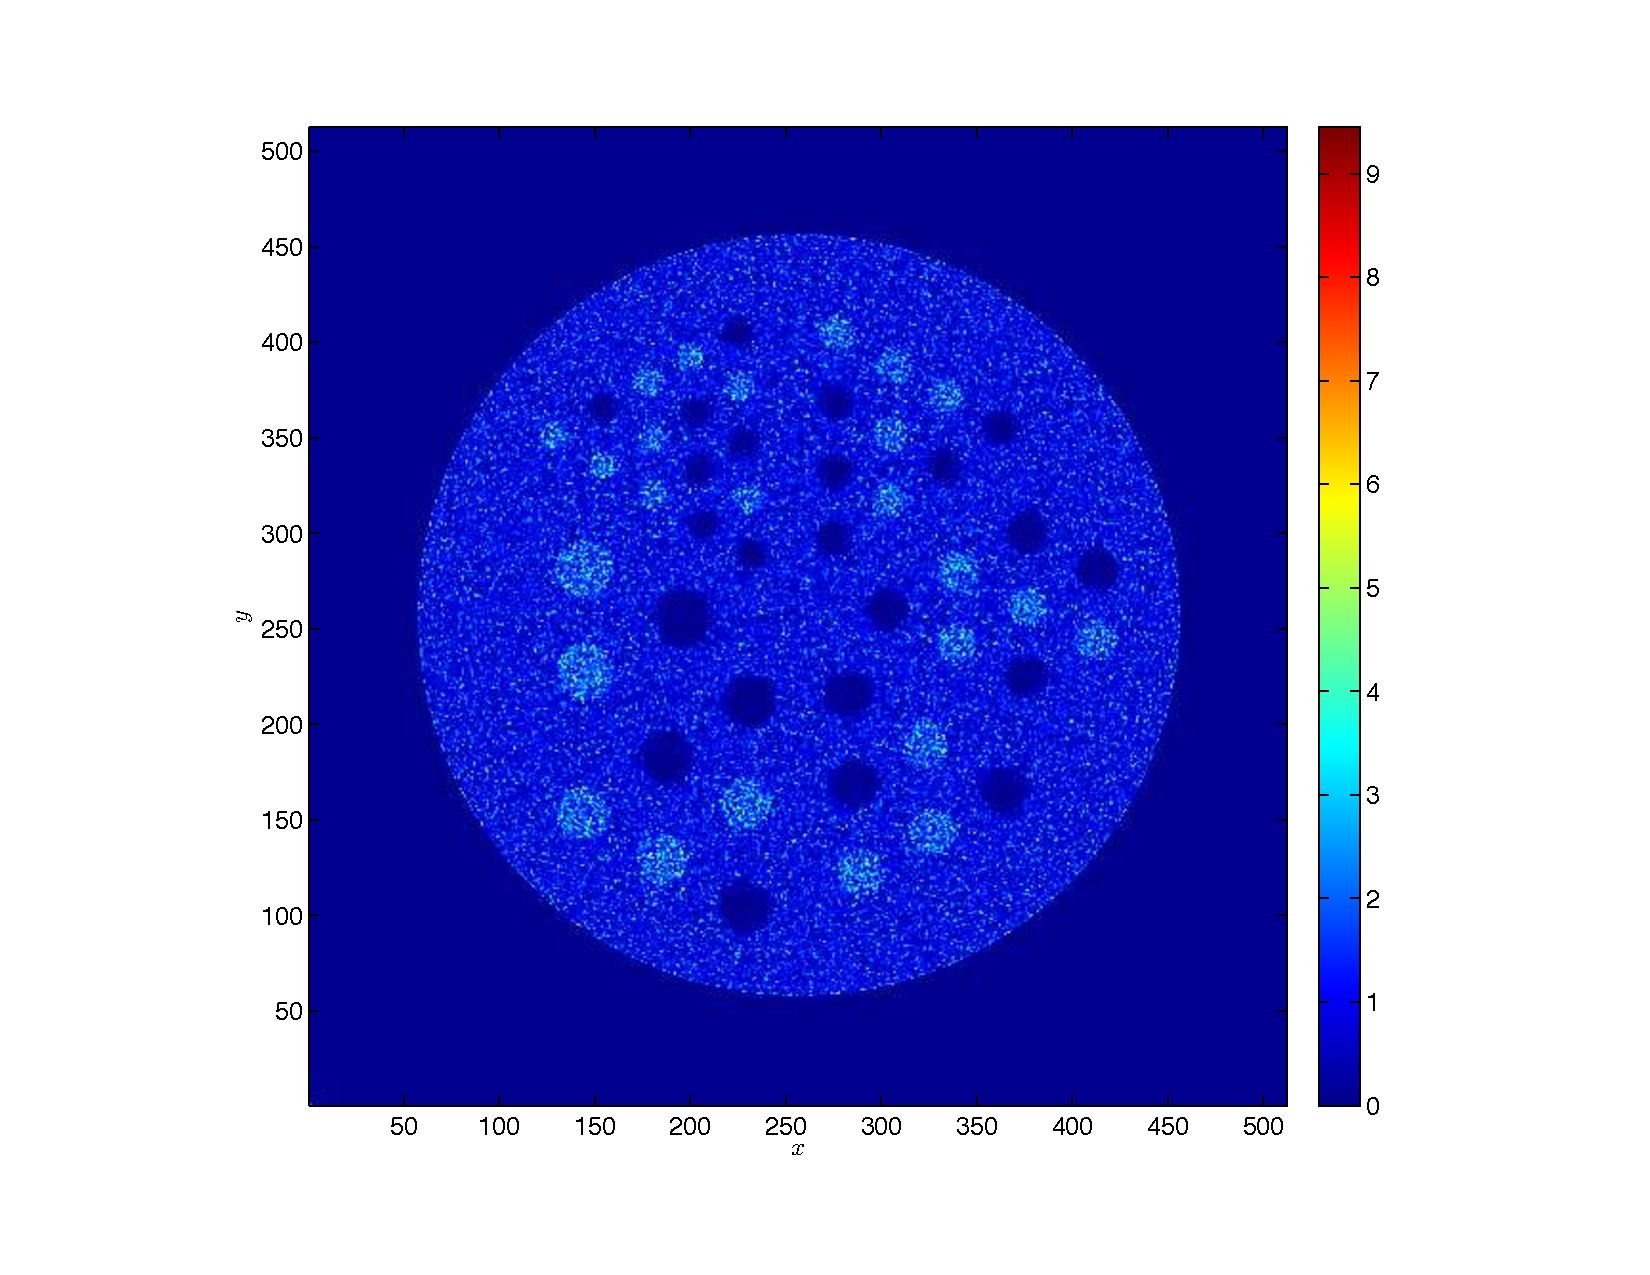
\includegraphics[width=\textwidth]{figures/OneSampleMLEM}
	\end{minipage}
	\begin{minipage}[b]{.43\linewidth}
 	  	\centering
 	  	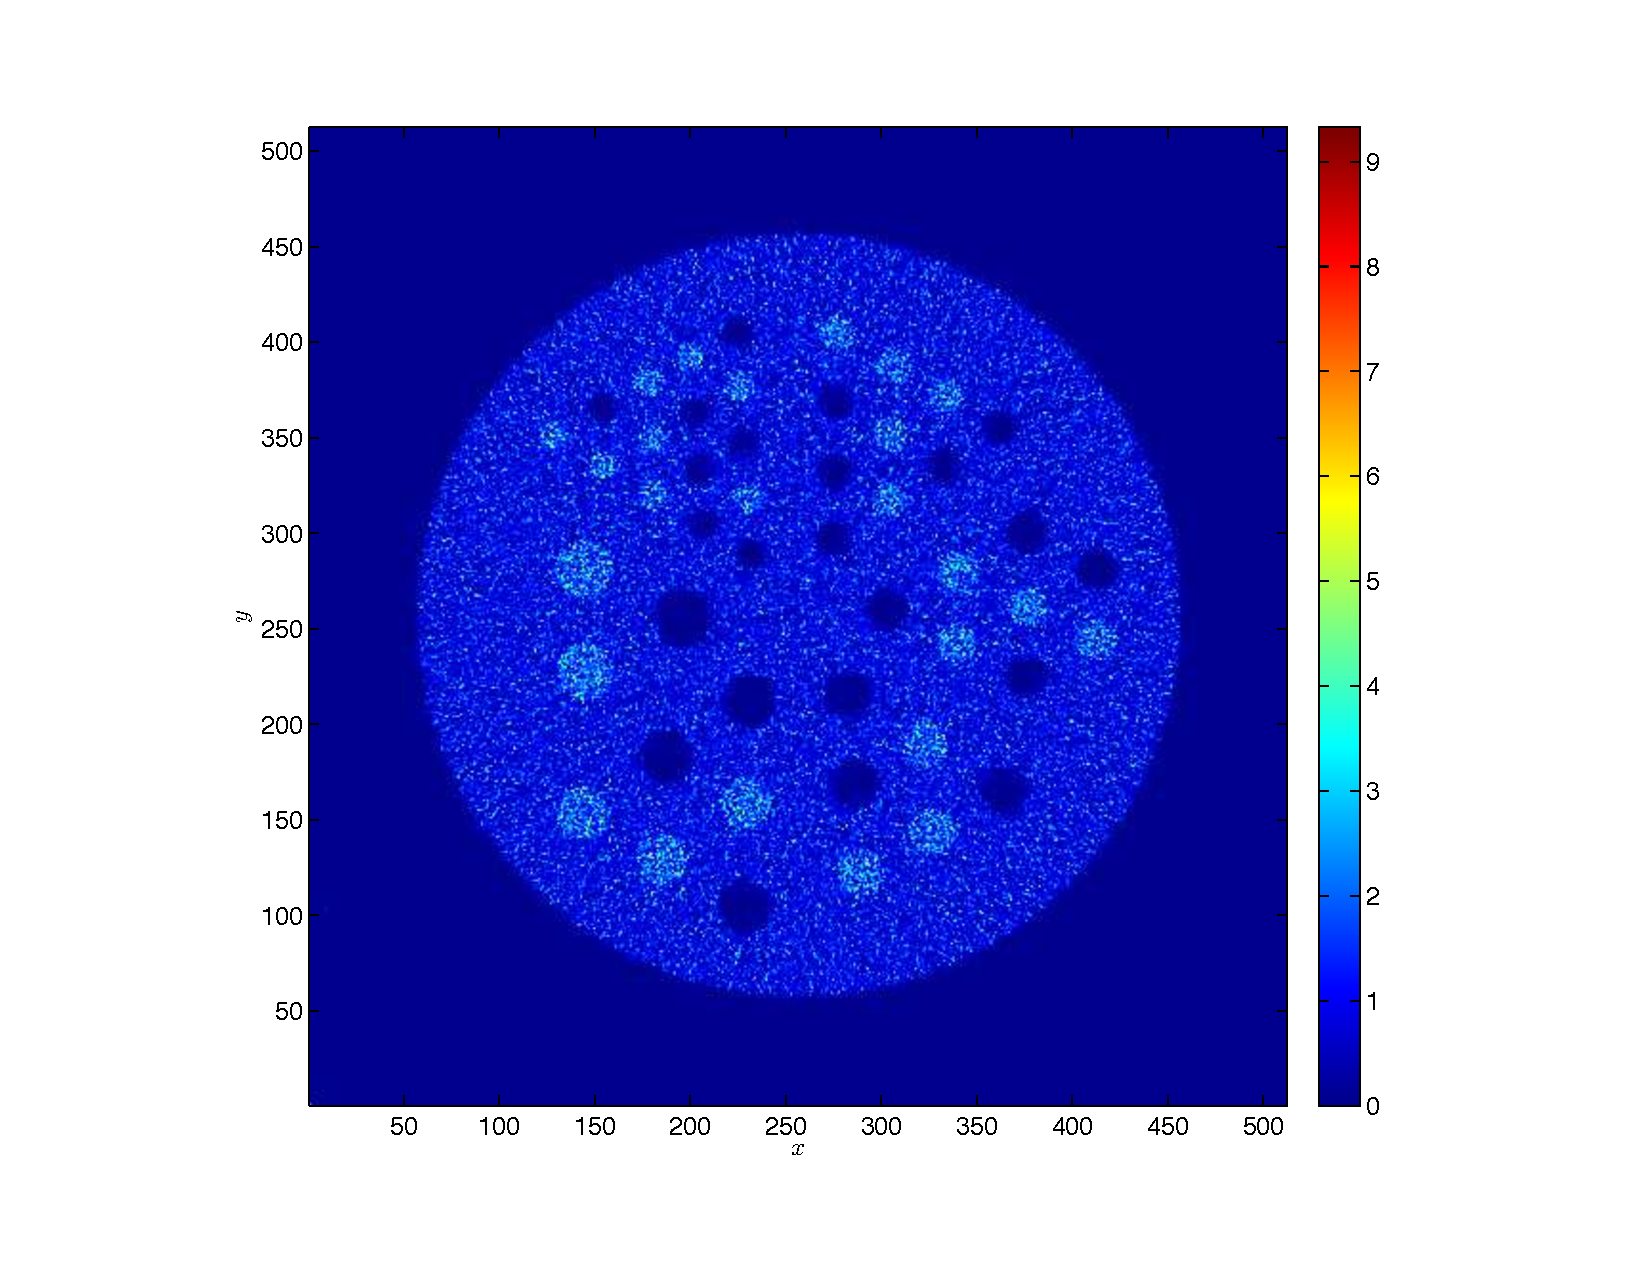
\includegraphics[width=\textwidth]{figures/OneSampleISRA}
	\end{minipage}
	\caption{\emph{($\rightarrow$ \ref{fig:a7}): The reconstruction of a single image with MLEM (left) and ISRA (right). As expected, the reconstructed images are less sharp than the expected images in figure \ref{fig:ResultsExpBiasVar200}.}}
	\label{fig:singleReconstruction}
\end{figure}


Visual comparison of the different images does not reveal any major differences between MLEM and ISRA. The expected value images, bias images and variance images are nearly identical. Their resolutions are comparable and their values in the different hot, cold and background regions of interest\footnote{Regions of interest = ROI, defined in figure \ref{fig:roi}} are similar. The only slightly notable difference is that the outer edge reconstructed by ISRA is a little fuzzier than with MLEM. This is notable as a ring around the phantom in the ISRA expected image and can also be noted as a region with a slight bias in the ISRA bias image. The edge of the ISRA variance image is also less clear cut than for the MLEM image. Remark also that the variance image closely ressembles the original image: hot regions have larger variances than cold regions.\\

\setlength\intextsep{0pt}
\begin{wrapfigure}{r}{0.42\textwidth}
	\centering 
	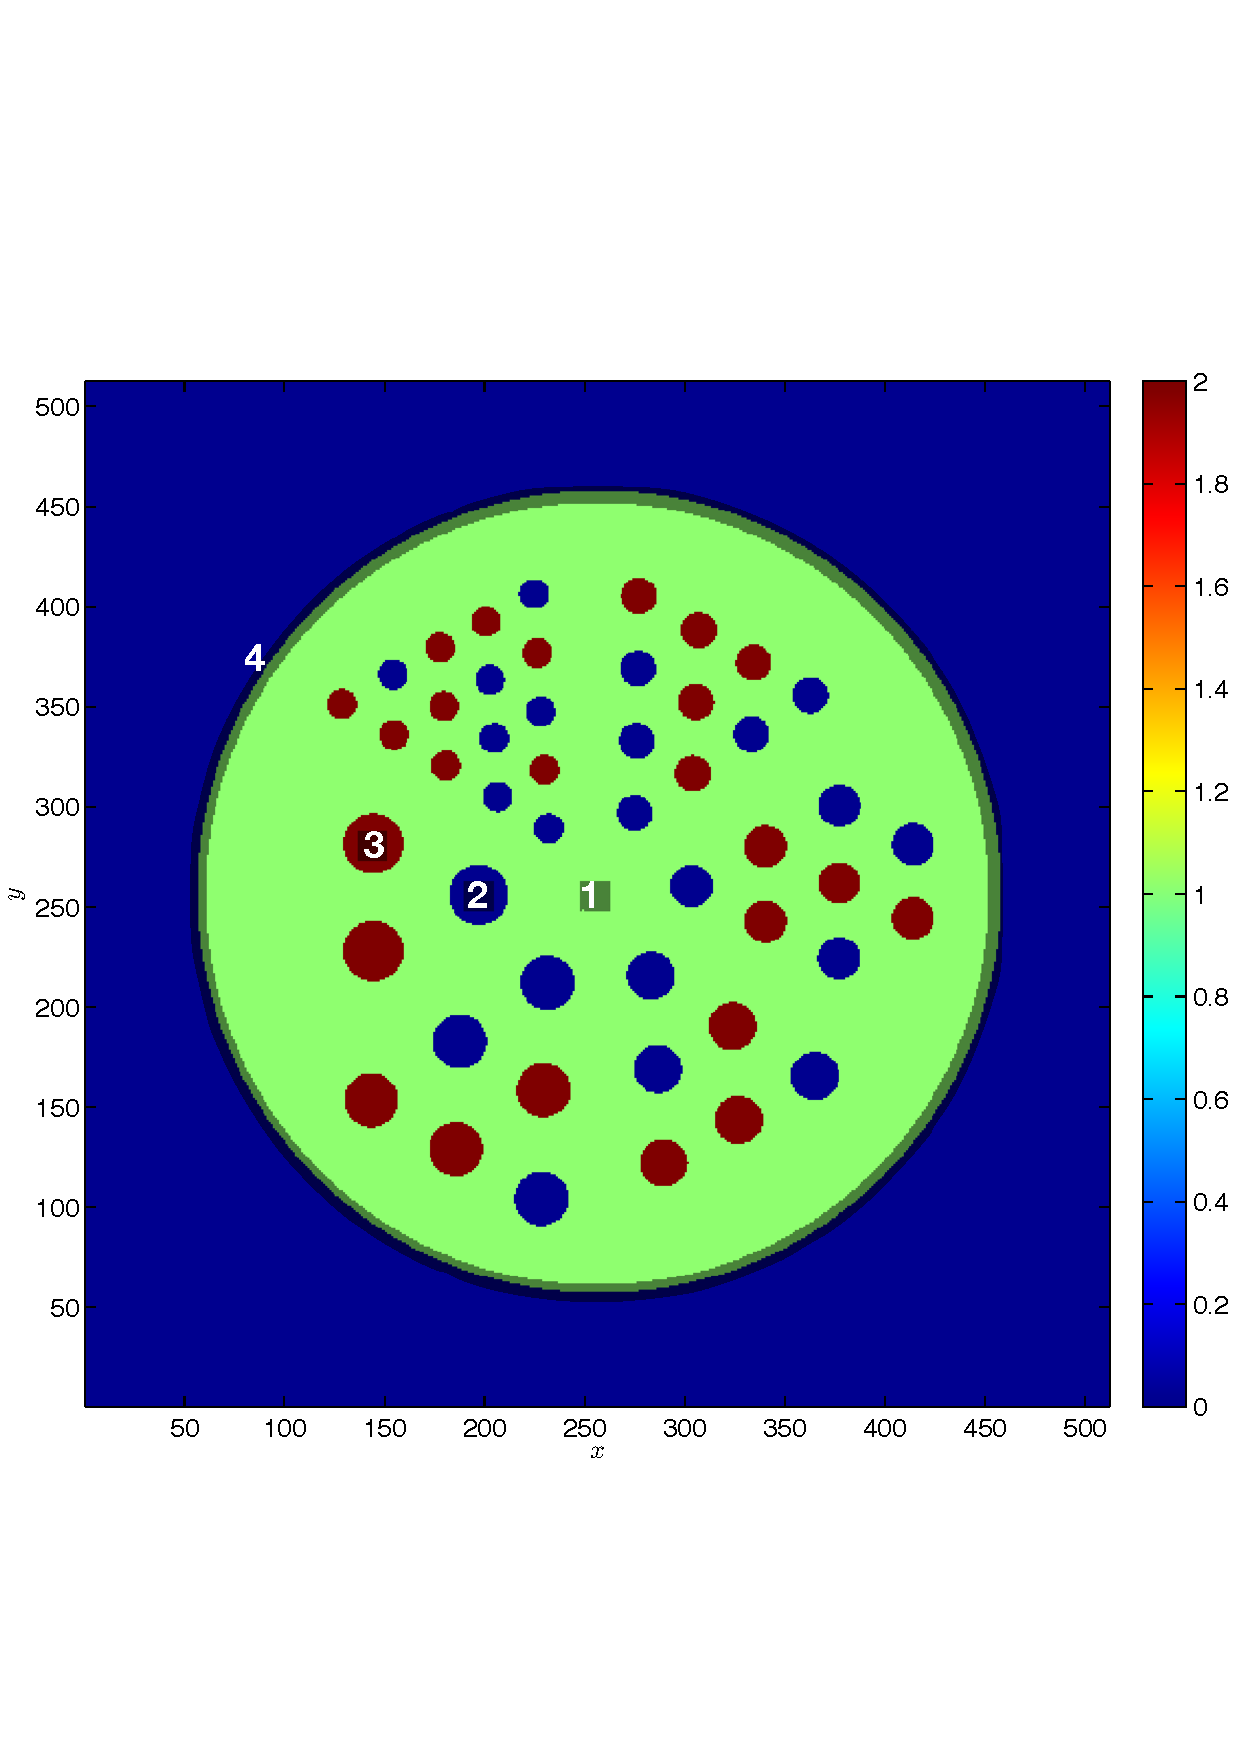
\includegraphics[width=.45\textwidth]{figures/DefRoi}
	\caption{\emph{($\rightarrow$ \ref{fig:a8}): Some specific regions of interest to be examined.}}
	\label{fig:roi}
\end{wrapfigure}
\intextsep\skip32
To get a more quantitative comparison of both algorithms, the expected value, bias and variance can be examined in some specific ROIs. The regions of interest that are examined are indicated as shaded regions in figure \ref{fig:roi}. ROI 1 is a sample of the background region, ROI 2 is the center of a cold region, ROI 3 is the center of a hot region and ROI 4 is a circular band containing the outer edge of the image which is overlapping into and outside of the image. All examined quantities are averaged over the ROIs number of pixels. The expected value is examined, and the trade-off between variance and bias.\bigbreak

The expected value, averaged over a ROI is computed as
\begin{align}
	<\hat x>_{roi} = \frac{1}{n}\left( \sum_{j=1}^{n} \hat x_j \right),\ \ \ \ \ \forall \hat x_j \in ROI
\end{align}

The evolution of the expected value as a function of the number of iterations is represented graphically in figure \ref{fig:ResultExpectedValue200}. It should be noted that:
\begin{itemize}
	\item MLEM and ISRA have nearly identical behaviour in the background, cold and hot regions.
	
	\item MLEM and ISRA converge slower in the cold regions than in the hot regions.
	
	\item ISRA performs less good than MLEM on the edge, though the difference gets smaller as the number of iterations increases.
	
	\item The expected values converge to their true values in the non-zero regions.
\end{itemize}

Figure \ref{fig:ResultsExpBiasVar200} and \ref{fig:ResultExpectedValue200} show that MLEM and ISRA exhibit slightly different behaviour though the differences are not significant enough to favor one algorithm over the other.\\
\setlength\intextsep{\savedintextsep}


The bias and the variance in each ROI can be examined simultaneously by plotting the average variance on the x-axis and the average bias on the y-axis for each iteration. This yields a plot where the variance and bias can be compared and the trade-off between both can be analysed. Results closer to (0,0) are better as they correspond to results with both a small variance and bias.\\

As could be expected from the previous results in figures \ref{fig:NoiselessReconstructionMLEM}, \ref{fig:NoiselessReconstructionISRA} and \ref{fig:ResultsExpBiasVar200}, the bias vs. variance plots are quite similar for MLEM and ISRA in the background, cold and hot regions. On the outer edge MLEM and ISRA exhibit significantly different behaviour: initially the bias increases rapidly for both MLEM and ISRA. This is because both algorithms start from a uniform guess of 1 everywhere. After a few iterations, the bias stabilises and starts to decrease, but it does so much faster for MLEM than for ISRA. On the other hand, the variance of both algorithms increases as the number of iterations increases, but the increase is faster for MLEM than for ISRA. For a variance of about 0.05 ISRA's bias is approximatively 4 times larger that MLEM's bias and for a variance of about 0.19 ISRA's bias is still approximatively 4 times larger that MLEM's bias. This leads to the conclusion that on the outer edge MLEM performs better than ISRA.\\
\setlength\intextsep{\savedintextsep}
\begin{figure}[H]
	\centering
	\makebox[\linewidth][c]{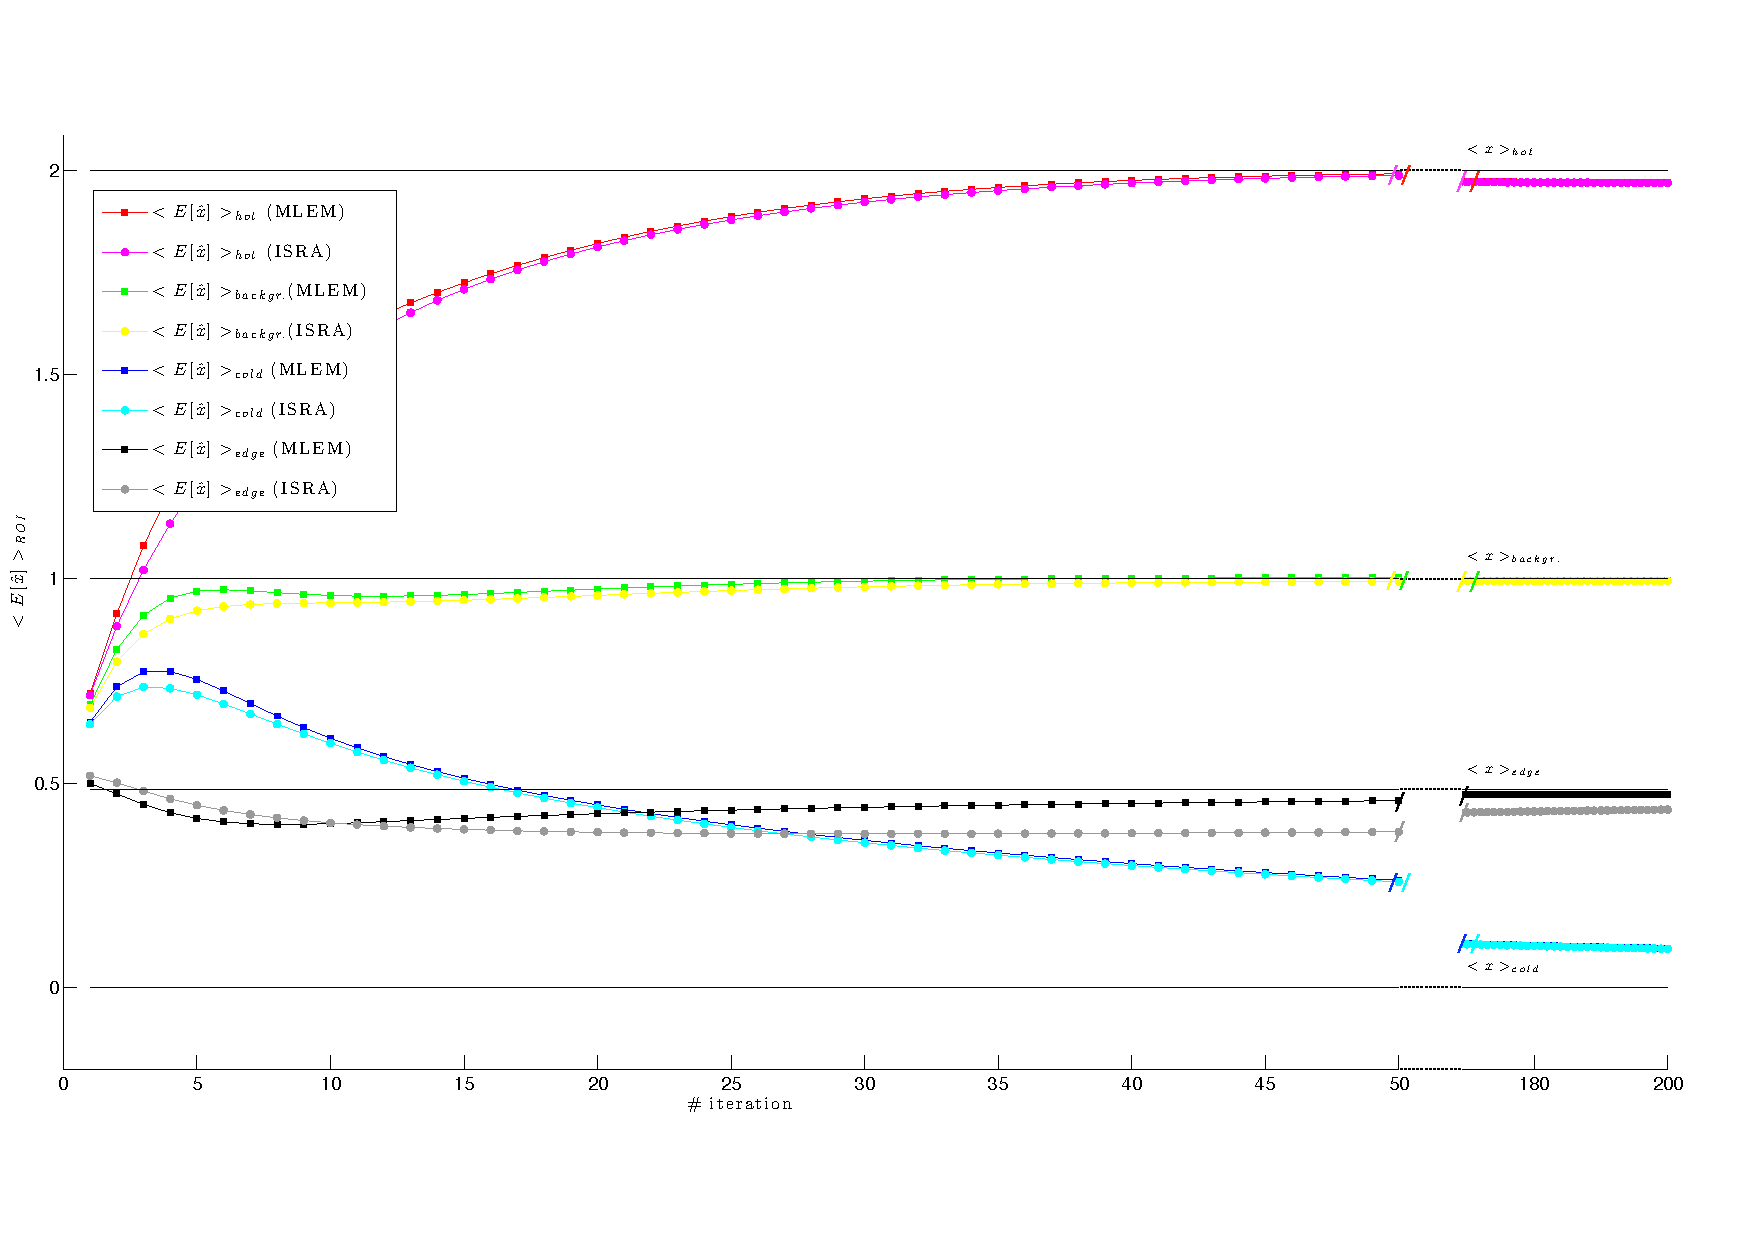
\includegraphics[width=1\linewidth]{figures/TheExpInRois.pdf}}
	\caption{\emph{The evolution of the expected value in each ROI as a function of the number of iterations. The black lines indicate the true value to which the different expected values should converge.}}
	\label{fig:ResultExpectedValue200}
\end{figure}

\begin{figure}[H]
	\centering
	\begin{minipage}[b]{\linewidth}
 		\centering
		\includegraphics[trim = 42mm 26mm 46mm 26mm, clip, 
width=\textwidth]{figures/BVsVBack.pdf}
	\end{minipage}	\hfill\newline
	\begin{minipage}[b]{\linewidth}
 	  	\centering
 	  	\includegraphics[trim = 42mm 26mm 46mm 26mm, clip, 
width=\textwidth]{figures/BVsVCold.pdf}
	\end{minipage}
\end{figure}
\begin{figure}[H]
	\centering
	\begin{minipage}[b]{\linewidth}
 		\centering
 		\includegraphics[trim = 42mm 26mm 46mm 26mm, clip, 
width=\textwidth]{figures/BVsVHot.pdf} 
	\end{minipage}	\hfill\newline
	\begin{minipage}[b]{\linewidth}
		\centering
		\includegraphics[trim = 42mm 26mm 46mm 26mm, clip, 
width=\textwidth]{figures/BVsVEdge.pdf} 
	\end{minipage}
	\caption{\emph{The bias vs. the variance in different ROIs.}}
\end{figure}




\subsection{2000 iterations}
The results in the previous section can be extended to 2000 iterations to study the algorithms' properties close to convergence. Due to computational limits and the huge amount of data and computational time required, it was not possible to store all intermediate iterations. Only the results at iteration 2000 are available. The expected images, bias images and variance images can be found in figure \ref{fig:ResultsExpBiasVar200} and the values of the average expected values, average biasses and average variances in each ROI can be found in table \ref{tab:Results2000It}.
\setlength\intextsep{\savedintextsep}
\begin{figure}[H]
\makebox[\textwidth][c]{
\begin{tabular}{ccc}
\subfloat{\includegraphics[trim = 40mm 20mm 40mm 15mm, clip, 
width=.43\textwidth]{figures/ExpMLEM2000}} &
\subfloat{\includegraphics[trim = 40mm 20mm 40mm 15mm, clip, 
width=.43\textwidth]{figures/BiasMLEM2000}} &
\subfloat{\includegraphics[trim = 40mm 20mm 40mm 15mm, clip, 
width=.43\textwidth]{figures/VarMLEM2000}} \\
\subfloat{\includegraphics[trim = 40mm 20mm 40mm 15mm, clip, 
width=.43\textwidth]{figures/ExpISRA2000}} &
\subfloat{\includegraphics[trim = 40mm 20mm 40mm 15mm, clip, 
width=.43\textwidth]{figures/BiasISRA2000}} &
\subfloat{\includegraphics[trim = 40mm 20mm 40mm 15mm, clip, 
width=.43\textwidth]{figures/VarISRA2000}} \\
\end{tabular}}
\caption{\emph{($\rightarrow$ \ref{fig:a9}): Results obtained after reconstruction with MLEM (top) and ISRA (bottom) with 2000 iterations, based on 40 different noise realisations.}}
	\label{fig:ResultsExpBiasVar2000}
\end{figure}

Again a visual comparison does not reveal any major differences between MLEM and ISRA.\\

A quantitative comparison between MLEM and ISRA can be performed by analysing different statistical properties of the reconstructed images. All the analysed properties are averaged over the different ROIs. The ROI averaged true value is
\begin{align}
	<x_{true}>_{roi}\ = \frac{1}{n}\left( \sum_{j=1}^{n} x_j\right),\ \ \ \ \ \forall x_j \in ROI
\end{align}

The ROI averaged expected value is
\begin{align}
	<E[\hat x]>_{roi}\ 
	&= \frac{1}{n} \left( \sum_{j=1}^{n} E[\hat x_j]\right)
	\nonumber\\
	&= \frac{1}{n} \left( \sum_{j=1}^{n} \left( \frac{1}{40}\sum_{i=1}^{40}(\hat x_j)_i \right)\right),\ \ \ \ \ \forall x_j \in ROI
\end{align}

where $(\hat x_j)_i$ is the $i$'th estimation of pixel $x_j$. The remaining examined properties are the bias, the variance, the standard deviation and the mean squared error. These are all computed in the same way as the ROI averaged expected value: the relevant property is first determined for each pixel individually and is then averaged over the ROI. This procedure allows a quantitative analysis of each property over the different ROIs.\\



As can be seen from the results in table \ref{tab:Results2000It}, all of the expected values are close to their true value and well within 1 standard deviation of that true value. Furthermore the expected values for MLEM and ISRA are nearly identical in the hot, cold and background regions. On the outer edge a difference of 6.5\% can be observed between MLEM and ISRA.\\

Small biasses can be observed in all regions, but only on the edge is there a significant difference between MLEM and ISRA. The bias for MLEM is almost 4 times smaller than ISRA's bias, but (opposed to the results after only 200 iterations) the variances are nearly identical for MLEM and ISRA. So after 2000 iterations MLEM preforms better that ISRA, though the differences are not that large.\\

Conclusions after 2000 iterations:
\begin{itemize}
	\item The expected values are almost equal to their true values.
	
	\item The results for MLEM and ISRA are nearly identical in the hot, cold and background regions.
	
	\item MLEM's bias is significantly smaller than ISRA's bias on the outer edge, but the variances are nearly identical.
\end{itemize}

These conclusions allow stating that MLEM yields a quantitatively slightly better image reconstruction than ISRA for this image after 2000 iterations and starting with a uniform initial guess.\\

\begin{table}[H]
\centering
\centerline{
\begin{tabular}{l|c|r|r|r|r|r|r|r|}
\cline{2-9}
\multirow{2}{*}{}& \multicolumn{8}{c|}{ROI}                                                                                                                                                                                                      \\ \cline{2-9} & \multicolumn{2}{c|}{Backgr.}& \multicolumn{2}{c|}{Cold}& \multicolumn{2}{c|}{Hot}& \multicolumn{2}{c|}{Edge}\\
\cline{2-9} & \multicolumn{1}{c:}{MLEM} & \multicolumn{1}{c|}{ISRA} & \multicolumn{1}{c:}{MLEM} & \multicolumn{1}{c|}{ISRA} & \multicolumn{1}{c:}{MLEM} & \multicolumn{1}{c|}{ISRA} & \multicolumn{1}{c:}{MLEM} & \multicolumn{1}{c|}{ISRA} \\ \hline
\multicolumn{1}{|l|}{$<x_{true}>_{ROI}$} & \multicolumn{1}{r:}{1.000}  & 1.000& \multicolumn{1}{r:}{0.000}& 0.000& \multicolumn{1}{r:}{2.000}& 2.000& \multicolumn{1}{r:}{0.483}& 0.483\\ \hline                   
\multicolumn{1}{|l|}{$<E[\hat x]>_{ROI}$} & \multicolumn{1}{r:}{0.991}  & 0.990& \multicolumn{1}{r:}{0.080}& 0.078& \multicolumn{1}{r:}{1.965}& 1.962& \multicolumn{1}{r:}{0.473}& 0.445\\ \hline
\multicolumn{1}{|l|}{$<b(\hat x)>_{ROI}$} & \multicolumn{1}{r:}{-0.009} & -0.010& \multicolumn{1}{r:}{0.078}& 0.078& \multicolumn{1}{r:}{-0.035}& -0.038& \multicolumn{1}{r:}{-0.010}& -0.038\\ \hline
\multicolumn{1}{|l|}{$<\sigma>_{ROI}$}  & \multicolumn{1}{r:}{1.554}  & 1.550& \multicolumn{1}{r:}{0.376}& 0.371& \multicolumn{1}{r:}{2.175}& 2.167& \multicolumn{1}{r:}{0.934}& 0.934\\ \hline
\multicolumn{1}{|l|}{$<var>_{ROI}$}  & \multicolumn{1}{r:}{2.415}  & 2.401& \multicolumn{1}{r:}{0.141}& 0.138& \multicolumn{1}{r:}{4.731}& 4.696& \multicolumn{1}{r:}{0.873}& 0.872\\ \hline
\multicolumn{1}{|l|}{$<MSE>_{ROI}$}  & \multicolumn{1}{r:}{2.415}  & 2.401& \multicolumn{1}{r:}{0.147}& 0.144& \multicolumn{1}{r:}{4.732}& 4.697& \multicolumn{1}{r:}{0.873}& 0.873\\ \hline
\end{tabular}}
\caption{\emph{The different relevant ROI averaged statistical properties after 2000 iterations.}}
\label{tab:Results2000It}
\end{table}




\subsubsection*{hypothesis test}
From table \ref{tab:Results2000It} it is clear that the expected values over the hot, cold and background ROIs are close to their true values over those ROIs. A hypothesis test is performed to determine whether these values are compatible. All tests are performed as a one sample t-test. The whole procedure is performed for the background region. Similar procedures are performed on the remaining ROIs.\\

Reminder: a region is defined as a set of pixels, see fig. \ref{fig:roi} and 40 images were reconstructed with each algorithm based on 40 sinograms with different noise realisations.\\ 




\subsubsection*{Individual pixel test}
The t-test is performed individually for each pixel of the ROI with $\upalpha$ = 1\%. The test is performed as follows: for each individual pixel $x_j$ in the ROI, a sample of 40 estimators $\hat x_j$ of $x_j$ is available from the 40 image reconstructions. For each $x_j$ in the ROI a null- and alternative hypothesis are stated\\

\textbf{H\subscript{0}} The estimated expected value of the activity in a pixel, $E[\hat x_{j}]$, is compatible with its true value $x_j$: $E[\hat x_{j}] = \overline{\hat x_{j}} = x_j = 1$.\\

\textbf{H\subscript{a}} The estimated expected value of the activity in a pixel, $E[\hat x_{j}]$, is \emph{not} compatible with its true value $x_j$: $E[\hat x_{j}] = \overline{\hat x_{j}} \neq x_j = 1$.\\


Based on the sample of 40 estimators for pixel $x_j$, the statistic $t(\hat x_{j}) = \frac{\overline{\hat x_{j}} - \mu_0}{s_{j} / \sqrt{n}}$ is determined with $\overline{\hat x_{j}}$ the sample mean, $\mu_0 = 1$ the population mean under the null-hypothesis, $s_j$ the sample standard deviation and $n = 40$ the number of observations. From the t-score, the p-value can be determined. A larger t-score leads to a smaller p-value. If the p-value is smaller than the significance level $\upalpha$, the null-hypothesis is rejected. 

To summarise the results over the ROI, the average p-value over the ROI is determined as $<p>_{ROI} = (1/n)\sum p(x_j)$. The test is performed and H\subscript{0} is accepted or rejected for each pixel individually. The whole ROI passes or fails the test if the average p-value over the ROI is larger than $\alpha$.
\setlength\intextsep{\savedintextsep}
\begin{table}[H]
\centerline{
\begin{tabular}{l|r|r|r|r|r|r|r|r|r|r|r|}
\cline{2-3} \cline{5-6} \cline{8-9} \cline{11-12}
                                                & \multicolumn{2}{c|}{Background}                       & \multicolumn{1}{c|}{} & \multicolumn{2}{c|}{Cold}                             & \multicolumn{1}{c|}{} & \multicolumn{2}{c|}{Hot}                              & \multicolumn{1}{c|}{} & \multicolumn{2}{c|}{Edge}                             \\ \cline{2-3} \cline{5-6} \cline{8-9} \cline{11-12} 
                                                & \multicolumn{1}{c|}{MLEM} & \multicolumn{1}{c|}{ISRA} & \multicolumn{1}{c|}{} & \multicolumn{1}{c|}{MLEM} & \multicolumn{1}{c|}{ISRA} & \multicolumn{1}{c|}{} & \multicolumn{1}{c|}{MLEM} & \multicolumn{1}{c|}{ISRA} & \multicolumn{1}{c|}{} & \multicolumn{1}{c|}{MLEM} & \multicolumn{1}{c|}{ISRA} \\ \cline{1-3} \cline{5-6} \cline{8-9} \cline{11-12} 
\multicolumn{1}{|l|}{\# pixels in ROI}          & 225                       & 225                       &                       & 225                       & 225                       &                       & 225                       & 225                       &                       & 6260                      & 6260                      \\ \cline{1-3} \cline{5-6} \cline{8-9} \cline{11-12} 
\multicolumn{1}{|l|}{\# pixels with p < $\upalpha$} & 11                        & 11                        &                       & 0                         & 0                         &                       & 3                         & 4                         &                       & 1487                      & 697                       \\ \cline{1-3} \cline{5-6} \cline{8-9} \cline{11-12} 
\multicolumn{1}{|l|}{\% of failure}             & 4.88\%                    & 4.88\%                    &                       & 0\%                       & 0\%                       &                       & 1.34\%                    & 1.78\%                    &                       & 23.75\%                   & 11.13\%                   \\ 
\cline{1-3} \cline{5-6} \cline{8-9} \cline{11-12} 
\multicolumn{1}{|l|}{alpha}               & 0.01                     & 0.01                     &                       & 0.01                     & 0.01                     &                       & 0.01                     & 0.01                     &                       & 0.01                     & 0.01                     \\ 
\multicolumn{1}{|l|}{ROI averaged p-value}               & 0.459                     & 0.456                     &                       & 0.134                     & 0.135                     &                       & 0.512                     & 0.514                     &                       & 0.311                     & 0.222                     \\ 
\cline{1-3} \cline{5-6} \cline{8-9} \cline{11-12} 
\multicolumn{1}{|l|}{H\subscript{0} accepted over ROI}                        & \multicolumn{1}{c|}{V}    & \multicolumn{1}{c|}{V}    & \multicolumn{1}{c|}{} & \multicolumn{1}{c|}{V}    & \multicolumn{1}{c|}{V}    & \multicolumn{1}{c|}{} & \multicolumn{1}{c|}{V}    & \multicolumn{1}{c|}{V}    & \multicolumn{1}{c|}{} & \multicolumn{1}{c|}{V}    & \multicolumn{1}{c|}{V}    \\ \cline{1-3} \cline{5-6} \cline{8-9} \cline{11-12} 
\end{tabular}}
\caption{\emph{The results of the individual pixel t-test on $E[\hat x_j] \overset{?}{=} \mu_0$} with $\upalpha$ = 1\%}
\label{tab:ttest}
\end{table}
\intextsep\skip32

When the hypothesis test is performed over each individual pixel before averaging, the null hypothesis - the expected values are compatible with their true values - is accepted over all ROIs.




\subsubsection*{ROI mean test}
Instead of performing a test on each individual pixel of the ROI and then averaging the p-value over the ROI, the order of operations can be inverted: a single test can be performed over the whole ROI by averaging the expected value of each individual pixel over the whole ROI and by then performing the t-test on the averaged expected value.\\

The null- and alternative hypothesis are\\

\textbf{H\subscript{0}} The average expected value of $\hat x_j$ over the background ROI is compatible with its true value: $\frac{1}{\#\ pixels}\sum E[\hat{x}_j] =\ <E[\hat x]>_{bckgr}\ = x_j = 1$.\\

\textbf{H\subscript{a}} The average expected value of $\hat x_j$ over the background ROI is \emph{not} compatible with its true value: $<E[\hat x]>_{bckgr}\ \neq x_j =1$.\\

For each reconstructed image, the average of the expected values of the estimators $\hat x_j$ is determined over the ROI. This produces a sample of 40 ROI means. From this sample, the statistic $t(E[\hat x]) = \frac{<E[\hat x]>_{bckgr} - \mu_0}{s / \sqrt{n}}$ is determined with $<E[\hat x]>_{bckgr}$ the sample mean, $\mu_0 = 1$ the population mean under the null-hypothesis, $s$ the sample standard deviation and $n = 40$ the number of observations.
\setlength\intextsep{\savedintextsep}
\begin{table}[H]
	\centerline{
	\begin{tabular}{l|r|r|r|r|r|r|r|r|r|r|r|}
\cline{2-3} \cline{5-6} \cline{8-9} \cline{11-12}
                                         & \multicolumn{2}{c|}{Background}                               & \multicolumn{1}{c|}{} & \multicolumn{2}{c|}{Cold}                                     & \multicolumn{1}{c|}{} & \multicolumn{2}{c|}{Hot}                                      & \multicolumn{1}{c|}{} & \multicolumn{2}{c|}{Edge}                                     \\ \cline{2-3} \cline{5-6} \cline{8-9} \cline{11-12} 
                                         & \multicolumn{1}{c|}{MLEM}     & \multicolumn{1}{c|}{ISRA}     & \multicolumn{1}{c|}{} & \multicolumn{1}{c|}{MLEM}     & \multicolumn{1}{c|}{ISRA}     & \multicolumn{1}{c|}{} & \multicolumn{1}{c|}{MLEM}     & \multicolumn{1}{c|}{ISRA}     & \multicolumn{1}{c|}{} & \multicolumn{1}{c|}{MLEM}     & \multicolumn{1}{c|}{ISRA}     \\ \cline{1-3} \cline{5-6} \cline{8-9} \cline{11-12} 
\multicolumn{1}{|l|}{$\upmu_0$}   & 1                             & 1                             &                       & 0                             & 0                             &                       & 2                             & 2                             &                       & 0.4831                        & 0.4831                        \\ \cline{1-3} \cline{5-6} \cline{8-9} \cline{11-12} 
\multicolumn{1}{|l|}{$\upalpha$}           & 0.01                          & 0.01                          &                       & 0.01                          & 0.01                          &                       & 0.01                          & 0.01                          &                       & 0.01                          & 0.01                          \\
\multicolumn{1}{|l|}{p-value}            & 0.382                         & 0.301                         &                       & 8.8e-25                       & 1.3e-24                       &                       & 0.00127                       & 0.00068                       &                       & 4.8e-20                       & 8.1e-40                       \\ \cline{1-3} \cline{5-6} \cline{8-9} \cline{11-12} 
\multicolumn{1}{|l|}{H\subscript{0} accepted}   & \multicolumn{1}{c|}{V} & \multicolumn{1}{c|}{V} & \multicolumn{1}{c|}{} & \multicolumn{1}{c|}{X} & \multicolumn{1}{c|}{X} & \multicolumn{1}{c|}{} & \multicolumn{1}{c|}{X} & \multicolumn{1}{c|}{X} & \multicolumn{1}{c|}{} & \multicolumn{1}{c|}{X} & \multicolumn{1}{c|}{X} \\ \cline{1-3} \cline{5-6} \cline{8-9} \cline{11-12} 
\end{tabular}}
\caption{\emph{The results of the ROI mean t-test on $<E[\hat x]>_{ROI}  \overset{?}{=} \mu_0$ with $\alpha = 1\%$.}}
\label{tab:ttest2}
\end{table}

The results in table \ref{tab:ttest} and in table \ref{tab:ttest2} lead to several conclusions:
\begin{itemize}
	\item The null hypothesis is accepted in all regions on the individual pixel level, but is rejected in the cold, hot and edge regions when averaged over the ROI. This counter-intuitive conclusion can be explained by considering the sample variances $s_j$ for the individual pixel test and $s$ for the ROI mean test.\newline
	For the individual pixel test the sample variance $s_j$ is the variance of the sample of 40 estimators $\hat x_j$ of pixel $x_j$. For a single pixel the variance is expected to be large.\newline
	For the ROI mean test the sample variance $s$ is the variance of the sample of 40 expected values averaged over the ROI. Because they are averaged, the variance is expected to be smaller.\newline
	A smaller variance leads to a larger t-score and a larger t-score leads to a smaller p-value. This explains why the null-hypothesis can not be rejected on the individual pixel level but can be when averaging over the ROI. Intuitively this is because the t-test favorises the null-hypothesis as long as no strong evidence is found against it. Because for the individual test the information passed to the t-test is not very precise (large variance), the evidence against the null-hypothesis is not very strong so it is accepted by default. When averaged over the ROI, the information passed to the t-test is much more precise (smaller variance) which yields stronger evidence against the null-hypothesis which explains why it can be rejected.
	
	\item The expected values over the ROIs are only compatible with their true values in the background ROI, both for MLEM and for ISRA. 
\end{itemize}


\chapter{Conclusion}
PET-scans are useful tools in medicine that allow probing the interior of a patient in a non-invasive way. PET is based on the emission of positrons through radioactive $\upbeta$\superscript{+} decay of properly chosen tracers or radio-pharmaceuticals. The emitted positrons react with nearby electrons and form $\upgamma\upgamma$ pairs, which can be detected by dedicated scintillation detectors. These scintillation detectors provide the raw data from which the PET image must be reconstructed.\\

The emission of positrons is known to be a Poisson process so it is reasonable to assume that the data collected by the detectors follows a Poisson distribution as well. Different methods to reconstruct the image based on the assumption of Poisson distributed data were discussed.

One important iterative image reconstruction algorithm is MLEM. Historically MLEM and variants such as OSEM have been used extensively in PET with good results. However, when performing full 3D scans, the number of LORs increases dramatically due to the possibility of cross-slice LORs. In such a situation MLEM can be computationally expensive because the memory requirements increase dramatically as well. An alternative iterative reconstruction algorithm - ISRA - was proposed to optimise the full 3D image reconstruction problem. The fundamental difference between MLEM and ISRA is that ISRA is based on the assumption of a Gaussian data distribution. One of the main points of this thesis was to determine whether assuming a Gaussian data distribution has a significant impact on the reconstruction process and quality.\\

Various analytical and statistical methods were discussed to reconstruct an image from PET data. The analytical method discussed was filtered backprojection. The statistical reconstruction methods discussed were based on a maximum likelihood method or based on a least squares method. 

The maximum likelihood method required some assumption on the distribution of the data. The obvious choices were Poisson or Gaussian data distributions. Maximum likelihood estimators assuming Poisson data (indicated by the subscript or abbreviation 'ML' when needed) were shown to exist and be derivable for some problems. Furthermore maximum likelihood estimators assuming Gaussian data (indicated 'LS') were also shown to exist and be derivable. These maximum likelihood estimators assuming a Gaussian data distribution were shown to always be equivalent to estimators derived through a least squares (LS) method. 2 iterative  algorithms were derived: MLEM, which assumes a Poisson data distribution and converges to ML estimators, and ISRA, which assumes a Gaussian data distribution and converges to constrained, non-negative LS estimators.\\

To verify that it is possible to reconstruct a simple image with ML and LS estimators derived with the maximal likelihood method assuming Poisson respectively Gaussian data, and to verify that the iterative reconstruction methods MLEM and ISRA do as expected converge to ML estimators, respectively constrained, non-negative LS estimators, a small problem consisting of only 2 pixels and 3 detectors along specific LORs was studied. The study of this toy problem revealed that it is possible to reconstruct a PET image using a maximum likelihood method assuming Poisson or Gaussian data, that it is possible to derive closed form expressions for the expected value, bias and variance of the reconstructed images and that MLEM converges as expected to ML estimators, and that ISRA converges as expected to constrained, non-negative LS estimators.\\

Finally a quantitative and qualitative comparison between MLEM and ISRA was performed on realistic data. The main point was to determine whether assuming a Gaussian data distribution had a significant impact on the reconstruction process and quality. 

One particular image of a Jaszczak phantom that can be considered to be representative of a generic PET problem was chosen to perform this analysis. The differences of reconstruction quality between MLEM and ISRA were minimal, but noticeable. In particular ISRA suffered from a decreased reconstruction quality on the outer edge of the image. MLEM and ISRA achieved comparable variances on the outer edge, but MLEM's bias was smaller. In the other regions that were studied, the differences between MLEM and ISRA were negligible.\\

One might wonder whether these small, but statistically noticeable differences really matter. Because PET-scan images are used in medicine to observe a patient' interior, one might be inclined to conclude that MLEM and ISRA  yield statistically different results, but that these results are barely, if at all, noticeable when visually examining the reconstructed images and that therefore for all practical purposes, MLEM and ISRA can be considered to achieve equal reconstruction qualities in comparable time and iteration number in 2D image reconstruction problems.




\subsubsection*{Further work}
Further work is needed to compare MLEM and ISRA in more detail. In particular the quantitative comparison between MLEM and ISRA should be extended to multiple different phantom images. It should also be performed on a larger data set consisting of more reconstructed images. In this case, only 40 images were used. Finally the reconstruction comparisons should also be performed on images with less and more data counts, and with less and more noise to determine whether the results found in this comparison are valid in general.

A similar analysis should also be performed on 3D reconstruction problems.




%----------------------------------------------------------------------------
%Appendix
%----------------------------------------------------------------------------

\appendix
\chapter{Large figures}
This appendix presents some important figures from chapter \ref{chpt:PETRecMethods} in a larger and more readable format to highlight some details which may not be clear on the smaller images.


\newpage
\begin{landscape}


\begin{figure}
\begin{minipage}[b]{.85\linewidth}
	\centering
	\centerline{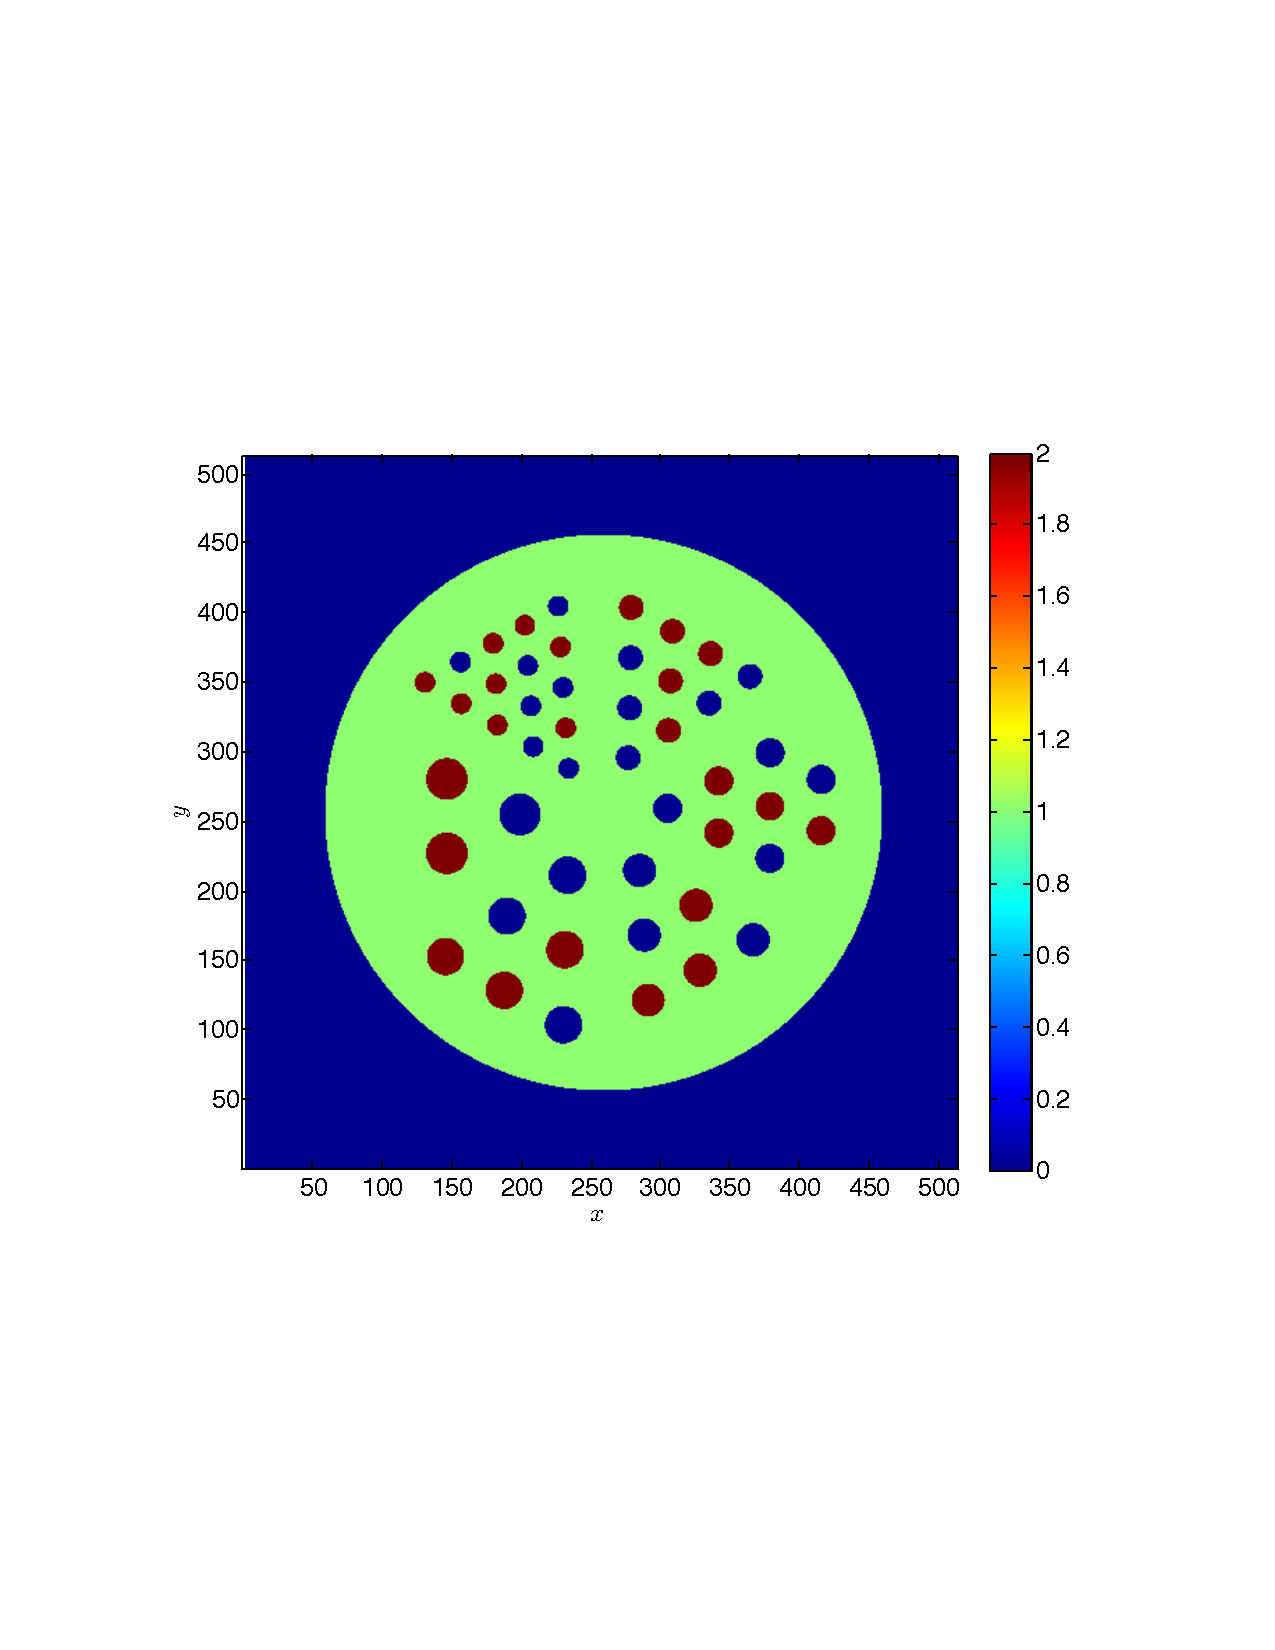
\includegraphics[width=\linewidth]{figures/JaszczakPhantom}}
	\caption{Large version of figure \ref{fig:jaszczak} right.\\
	The true 2D image of the Jaszczak phantom that will be used in this chapter. Remark the uniform background of the cylinder in green (activity = 1), the hot regions in red (activity = 2) and the cold regions in blue (activity = 0).}
	\label{fig:a1}
	\end{minipage}
\end{figure}
\bigbreak
\clearpage
\newpage




\begin{figure}
\begin{minipage}[b]{.85\linewidth}
	\centering
	\centerline{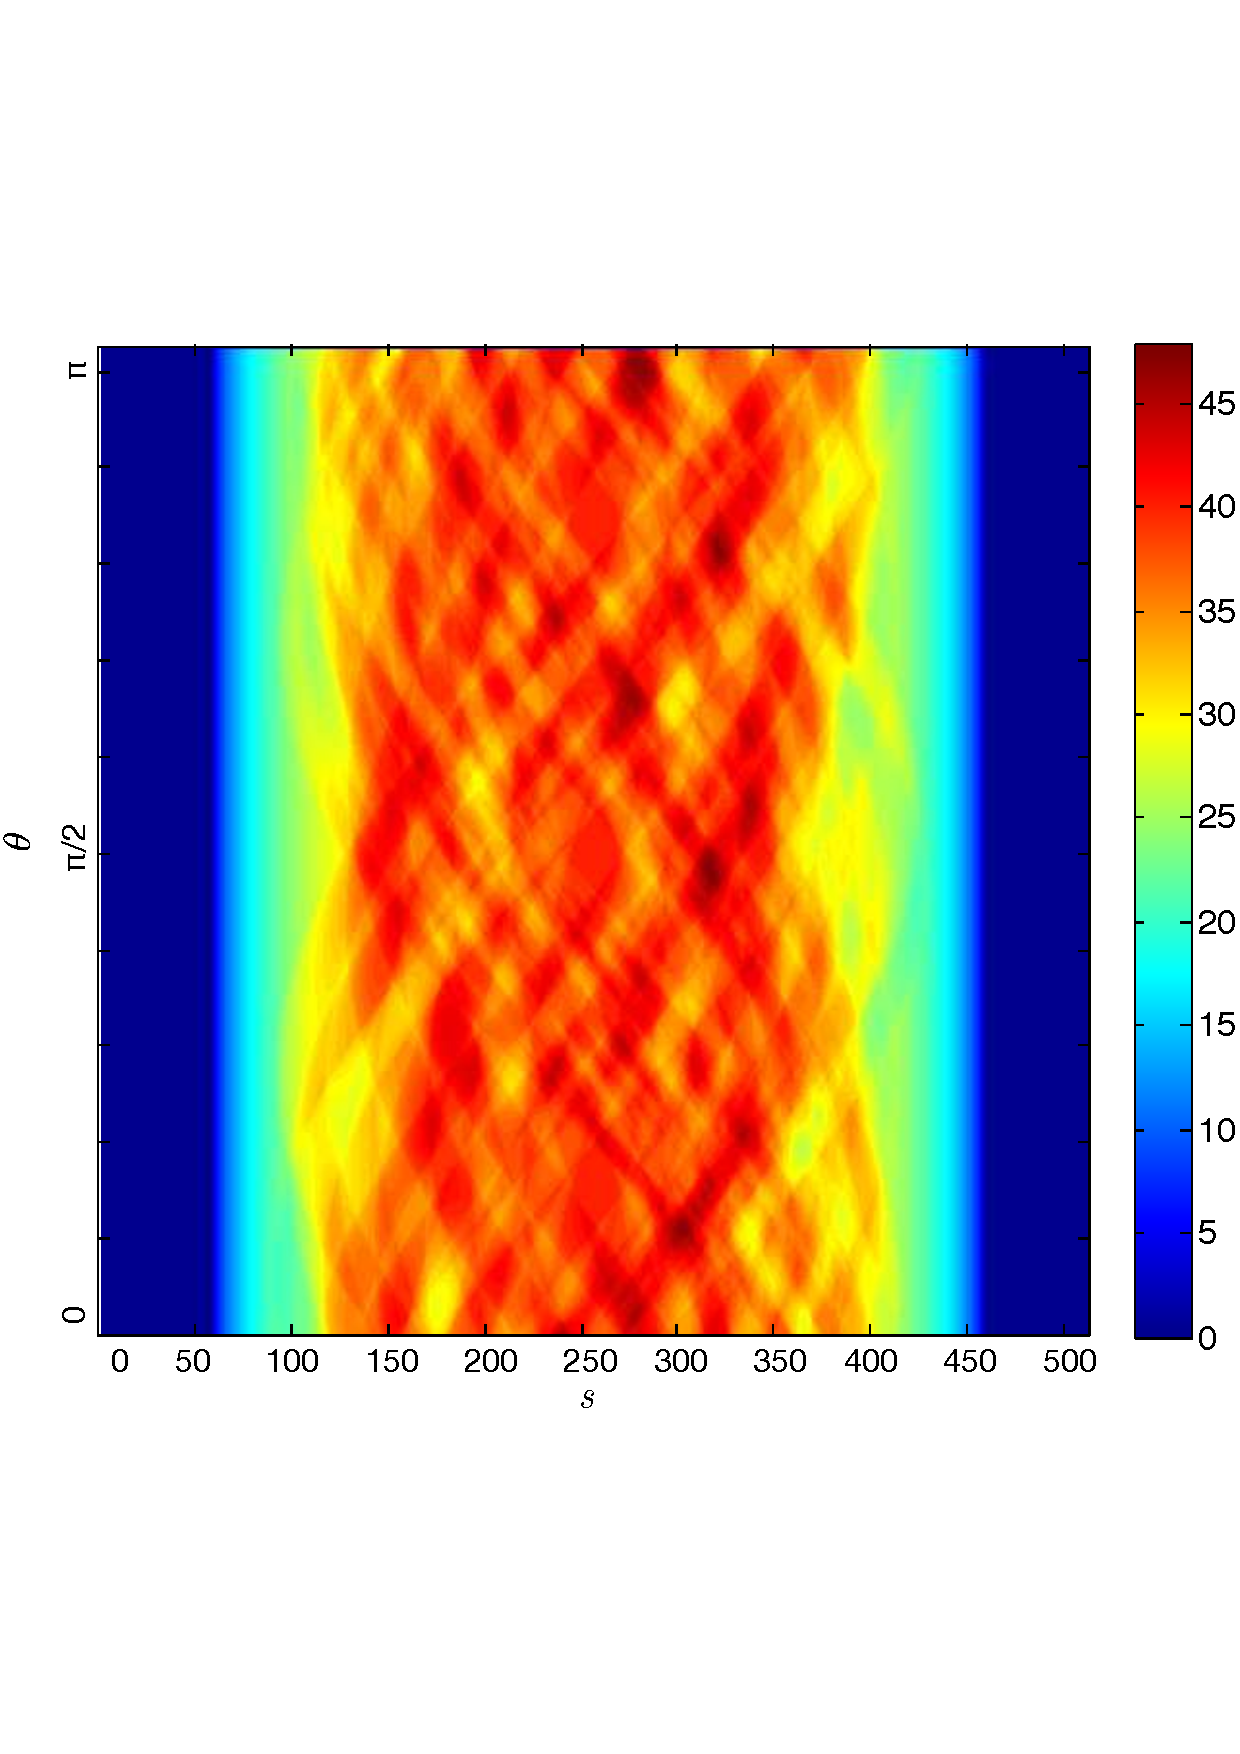
\includegraphics[width=\linewidth]{figures/sinogram}}	
	\caption{Large version of figure \ref{fig:sinogram}\\
	The noiseless sinogram of the Jaszczak phantom.}
	\label{fig:a2}
	\end{minipage}
\end{figure}
\bigbreak
\clearpage
\newpage




\begin{figure}[h]
		\centerline{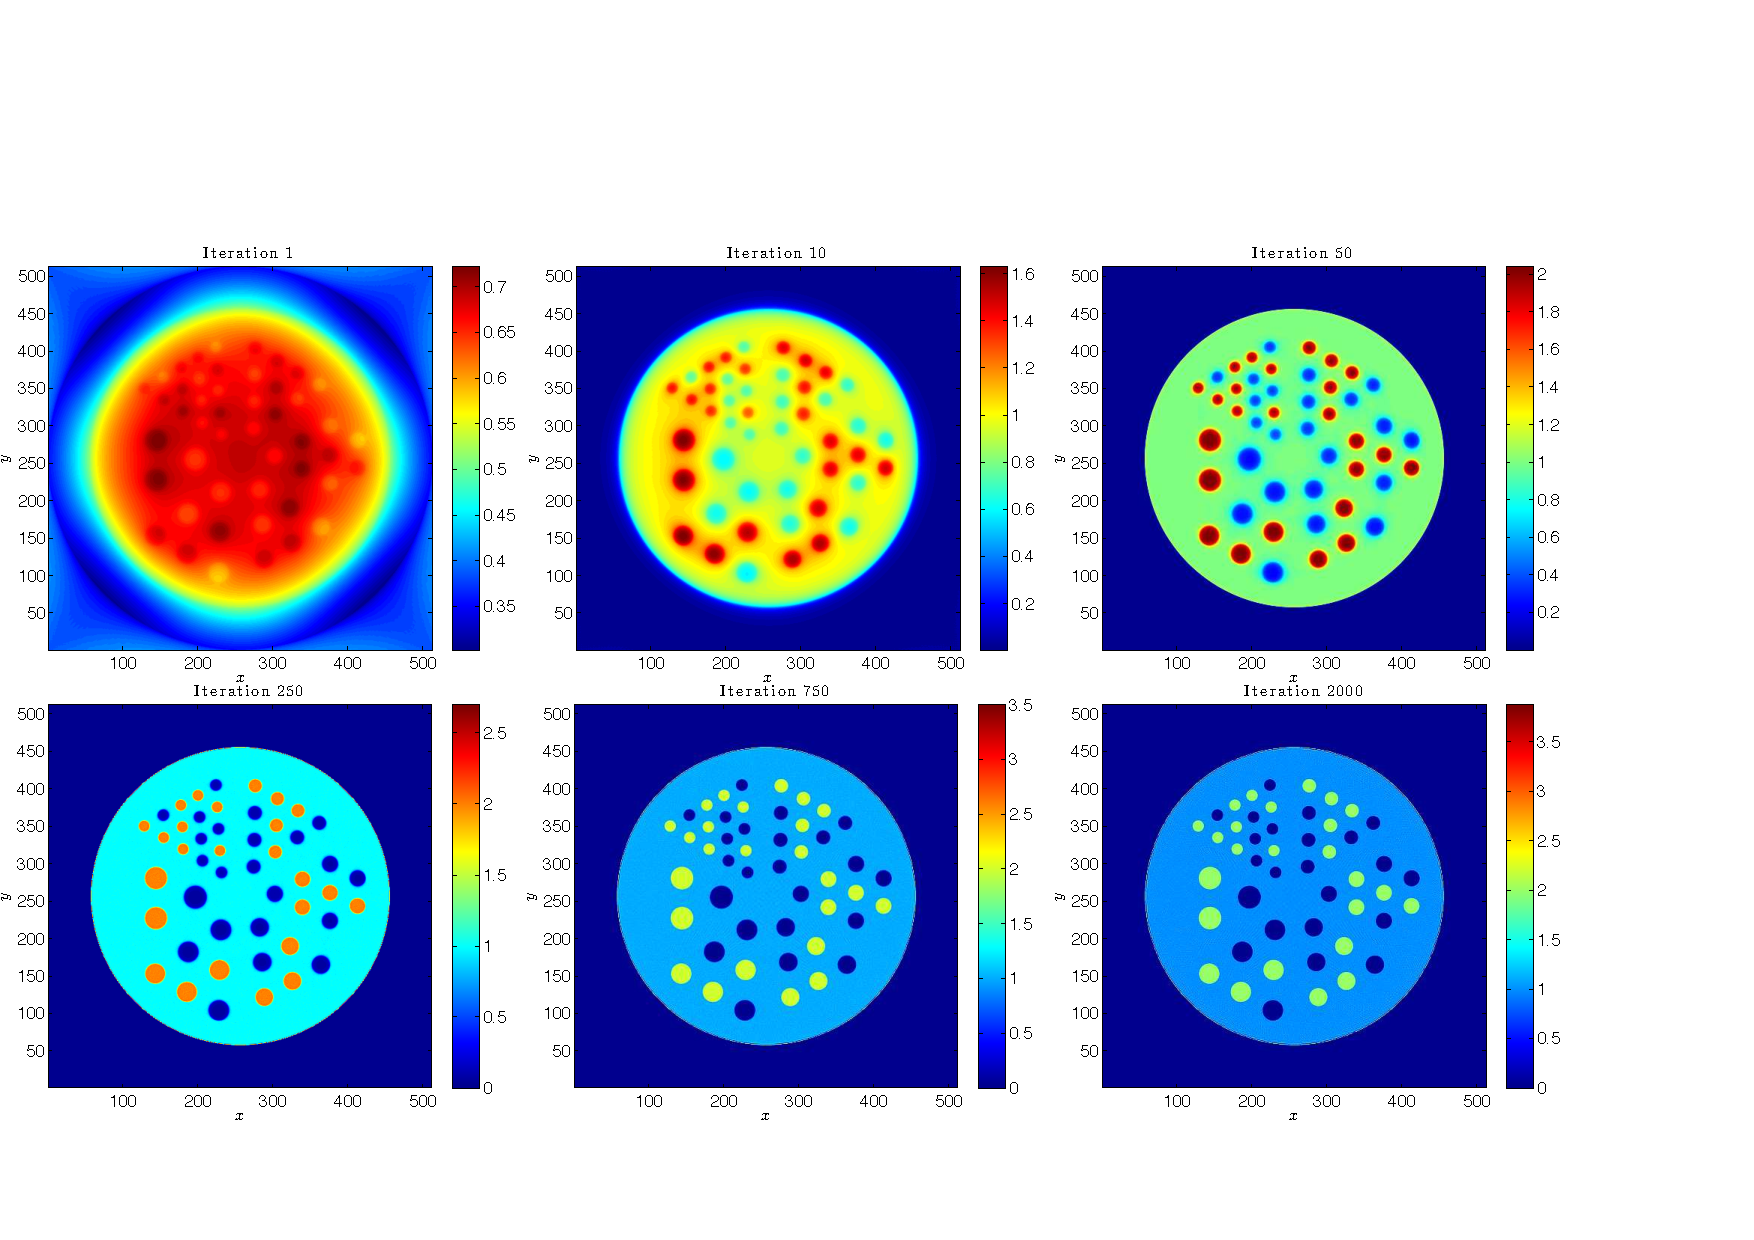
\includegraphics[width=1.08\linewidth]{figures/Appendix3}}
		\caption{Large version of figure \ref{fig:NoiselessReconstructionMLEM}\\
	The iterative image reconstruction of the Jaszczak phantom with MLEM starting from the exact sinogram in figure \ref{fig:sinogram}.}
		\label{fig:a3}
\end{figure}
\bigbreak
\clearpage
\newpage




\begin{figure}[h]
	\centerline{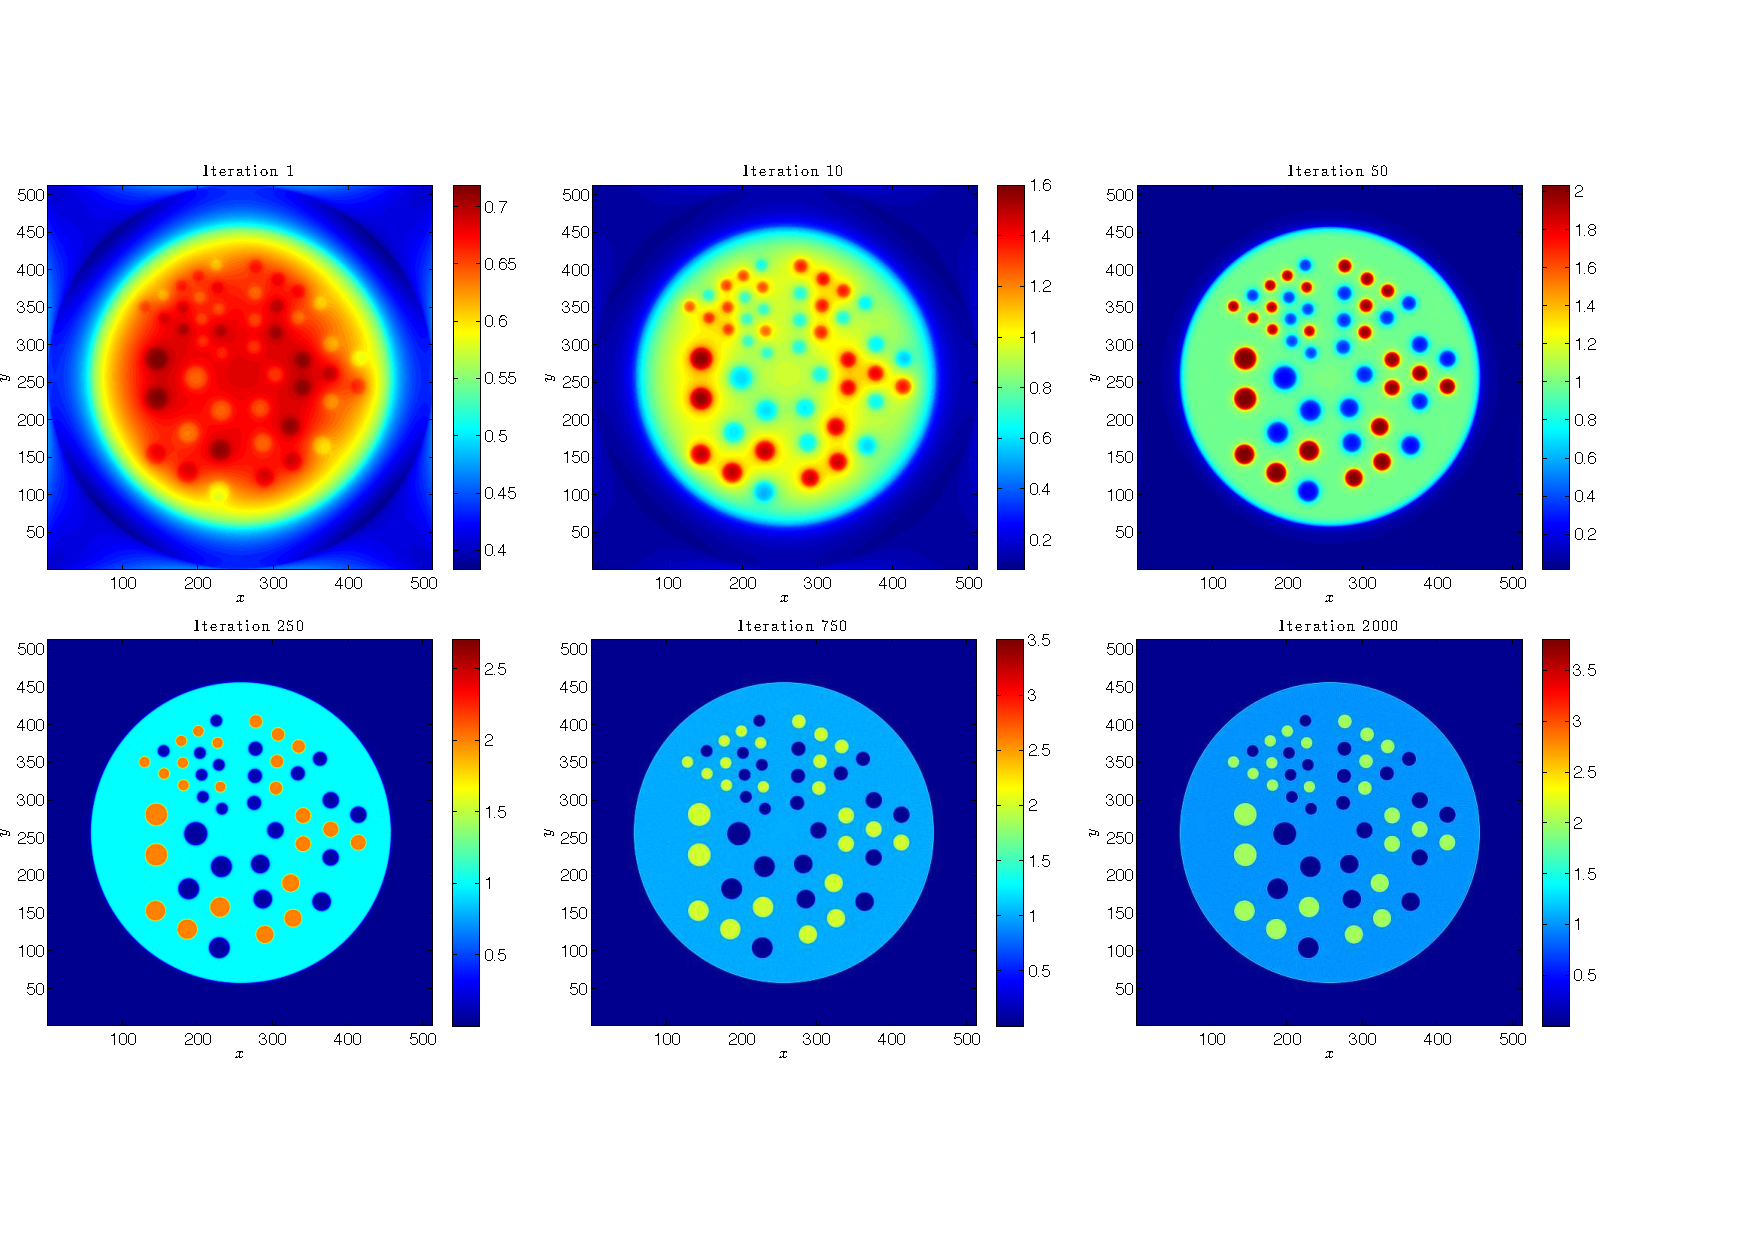
\includegraphics[width=1.08\linewidth]{figures/Appendix4}}
	\caption{Large version of figure \ref{fig:NoiselessReconstructionISRA}\\
	The iterative image reconstruction of the Jaszczak phantom with ISRA starting from the exact sinogram in figure \ref{fig:sinogram}.}
	\label{fig:a4}
\end{figure}
\bigbreak
\clearpage
\newpage




\begin{figure}
\begin{minipage}[b]{.85\linewidth}
	\centering
	\centerline{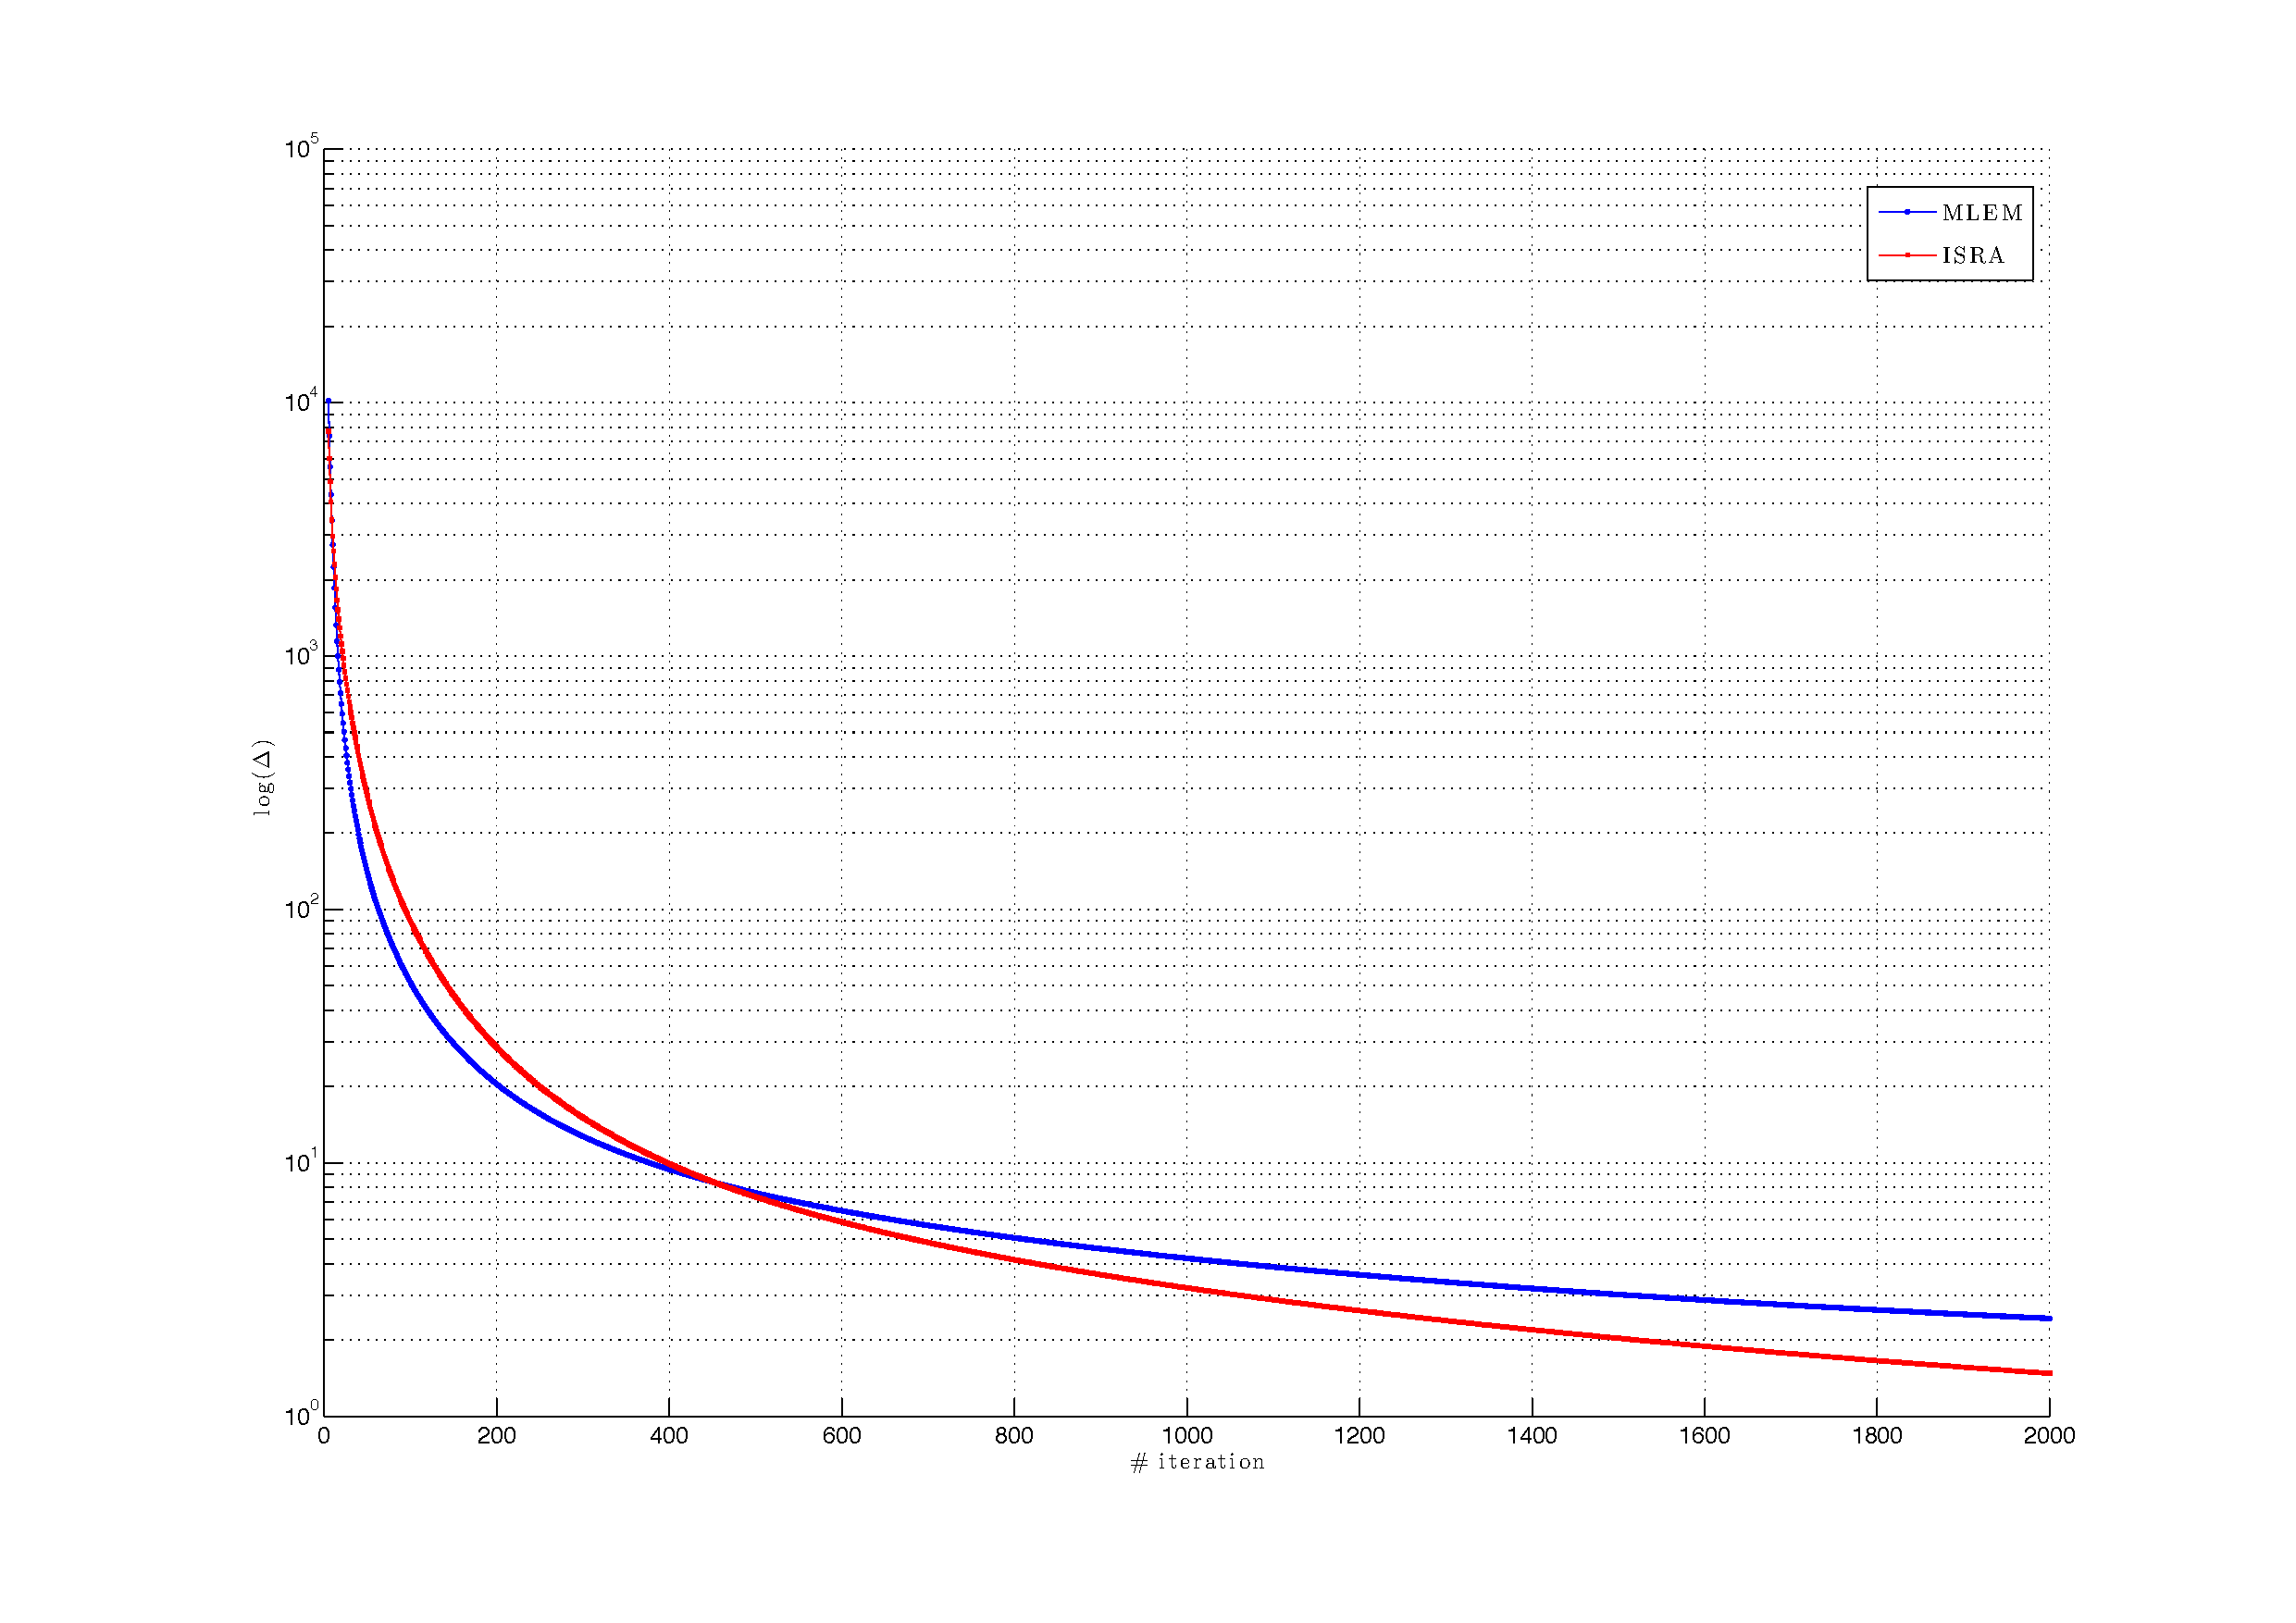
\includegraphics[width=\linewidth]{figures/RateOfConvergence.pdf}}
	\caption{Large version of figure \ref{fig:RateOfConvergence} right.\\
	The rate of convergence for MLEM (blue) and ISRA (red).}
	\label{fig:a45}
	\end{minipage}
\end{figure}
\bigbreak
\clearpage
\newpage





\begin{figure}[h]
\centering
	\centerline{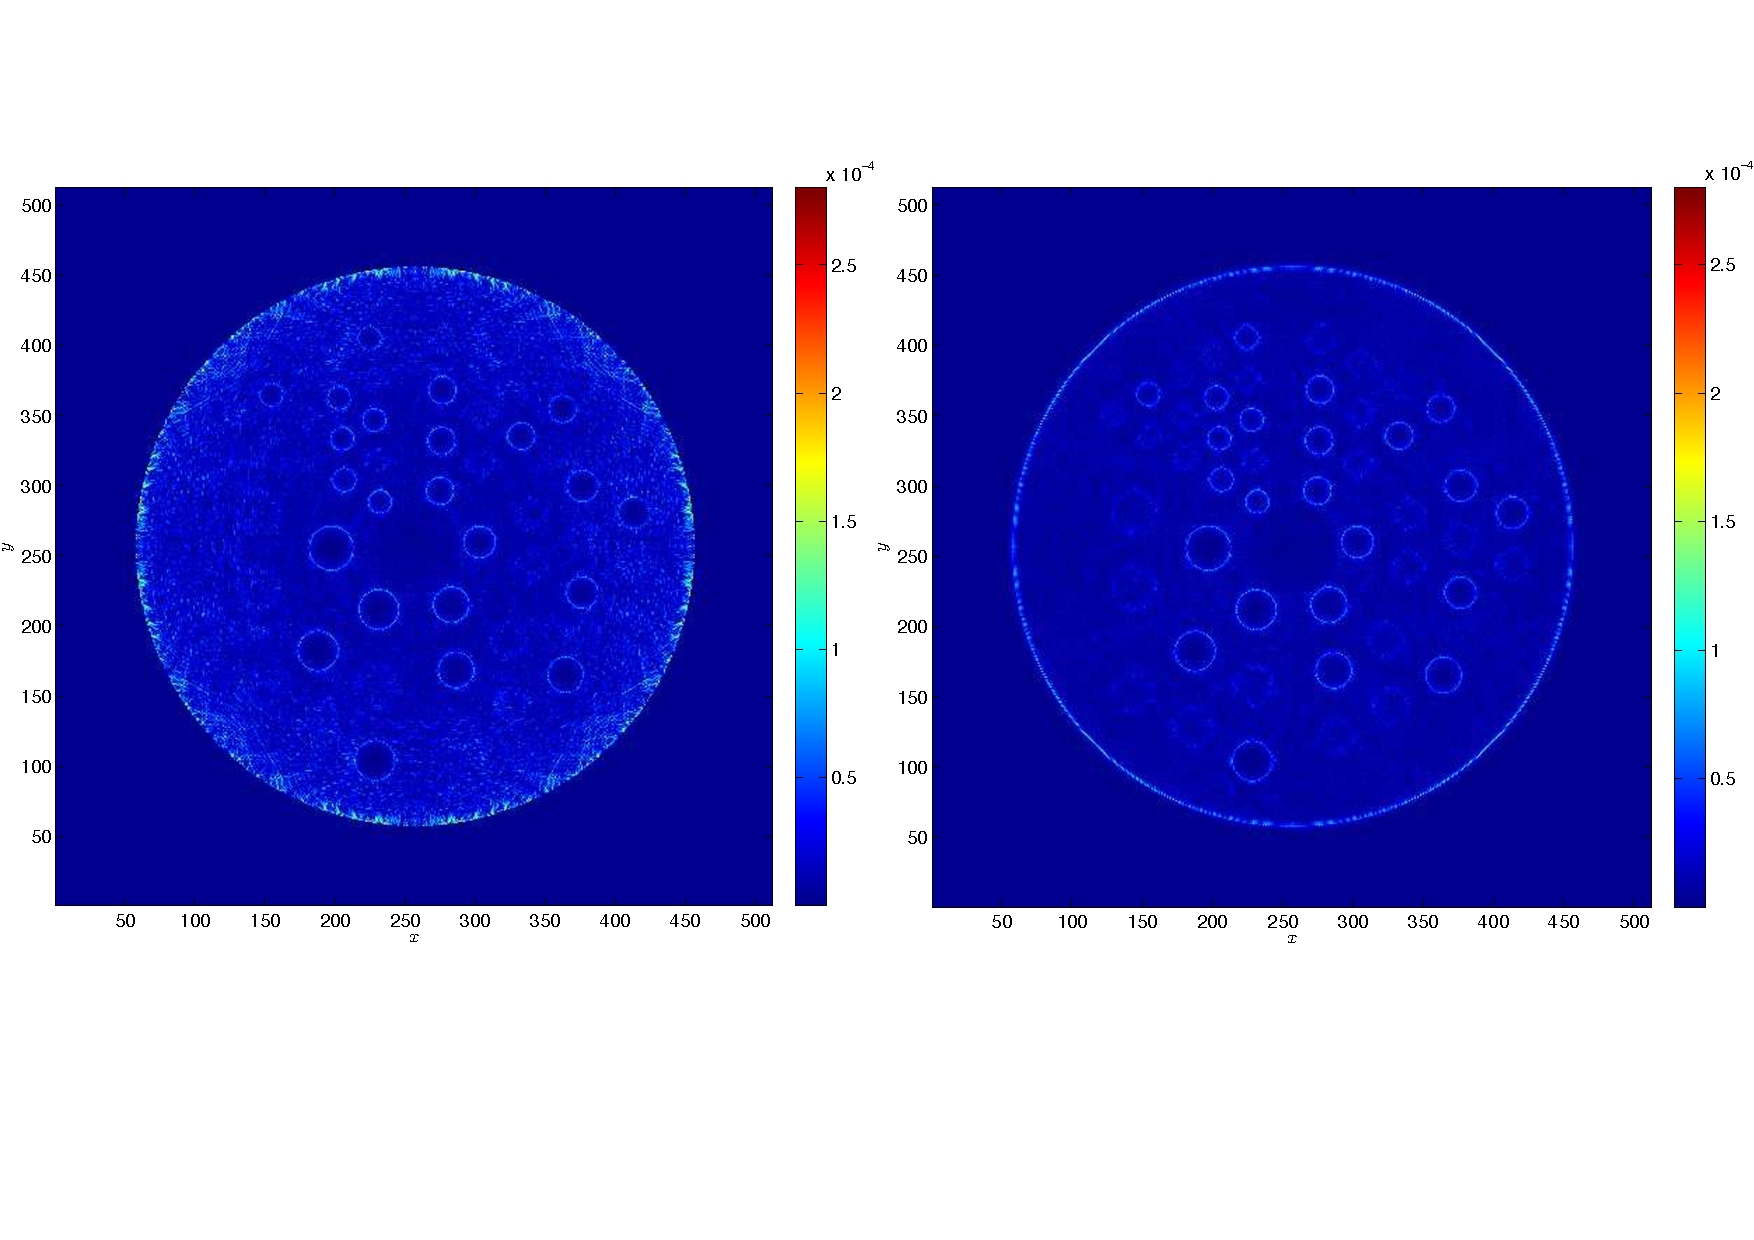
\includegraphics[width=1.01\linewidth]{figures/Appendix5}}
	\caption{Large version of figure \ref{fig:AlgorithmConvergenceTest}\\
	The difference between iteration 1999 and 2000 for MLEM (left) and ISRA (right).}
	\label{fig:a5}
\end{figure}
\bigbreak
\clearpage
\newpage




\begin{figure}[h]
	\centerline{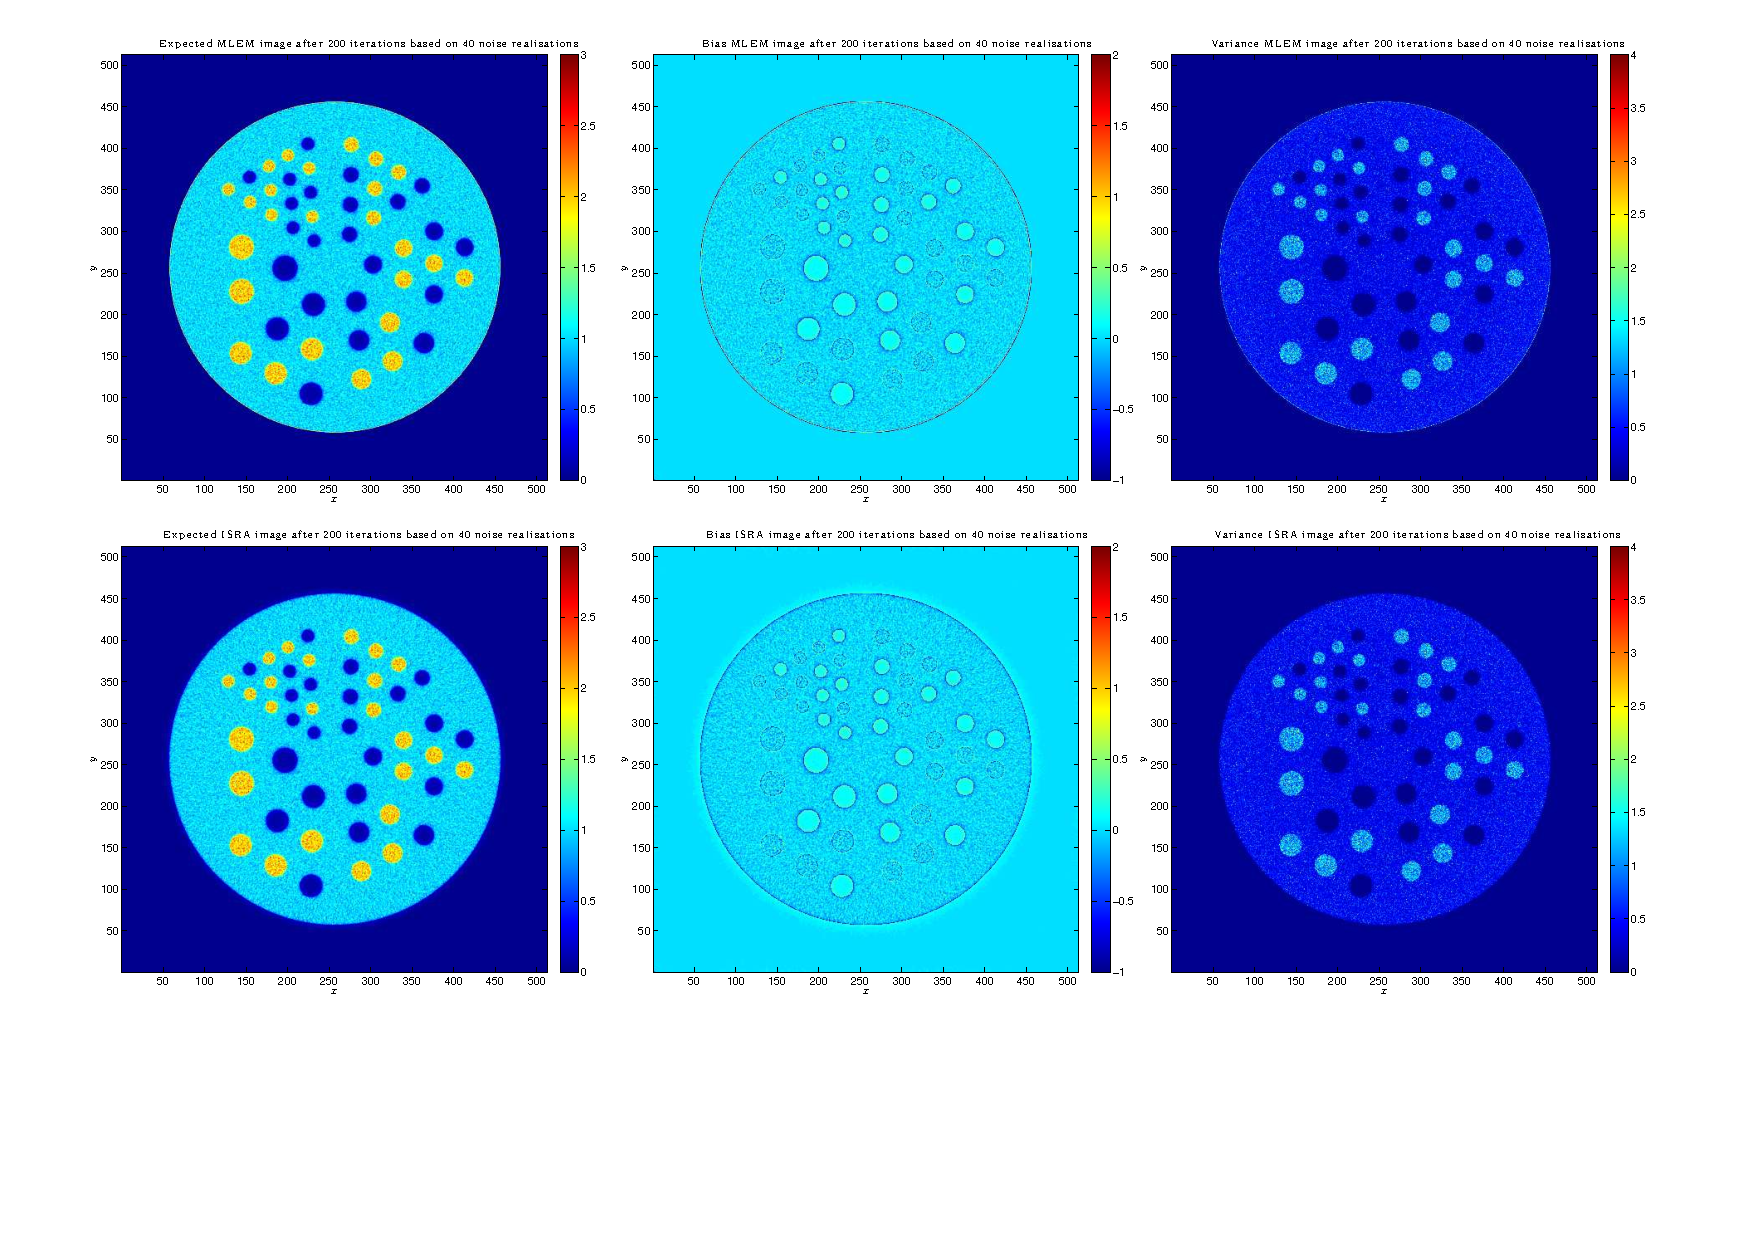
\includegraphics[width=1.08\linewidth]{figures/Appendix6}}
	\caption{Large version of figure \ref{fig:ResultsExpBiasVar200}\\
	Results obtained after reconstruction with MLEM (top) and ISRA (bottom) with 200 iterations, based on 40 different noise realisations.}
	\label{fig:a6}
\end{figure}
\bigbreak
\clearpage
\newpage




\begin{figure}[h]
\centering
	\centerline{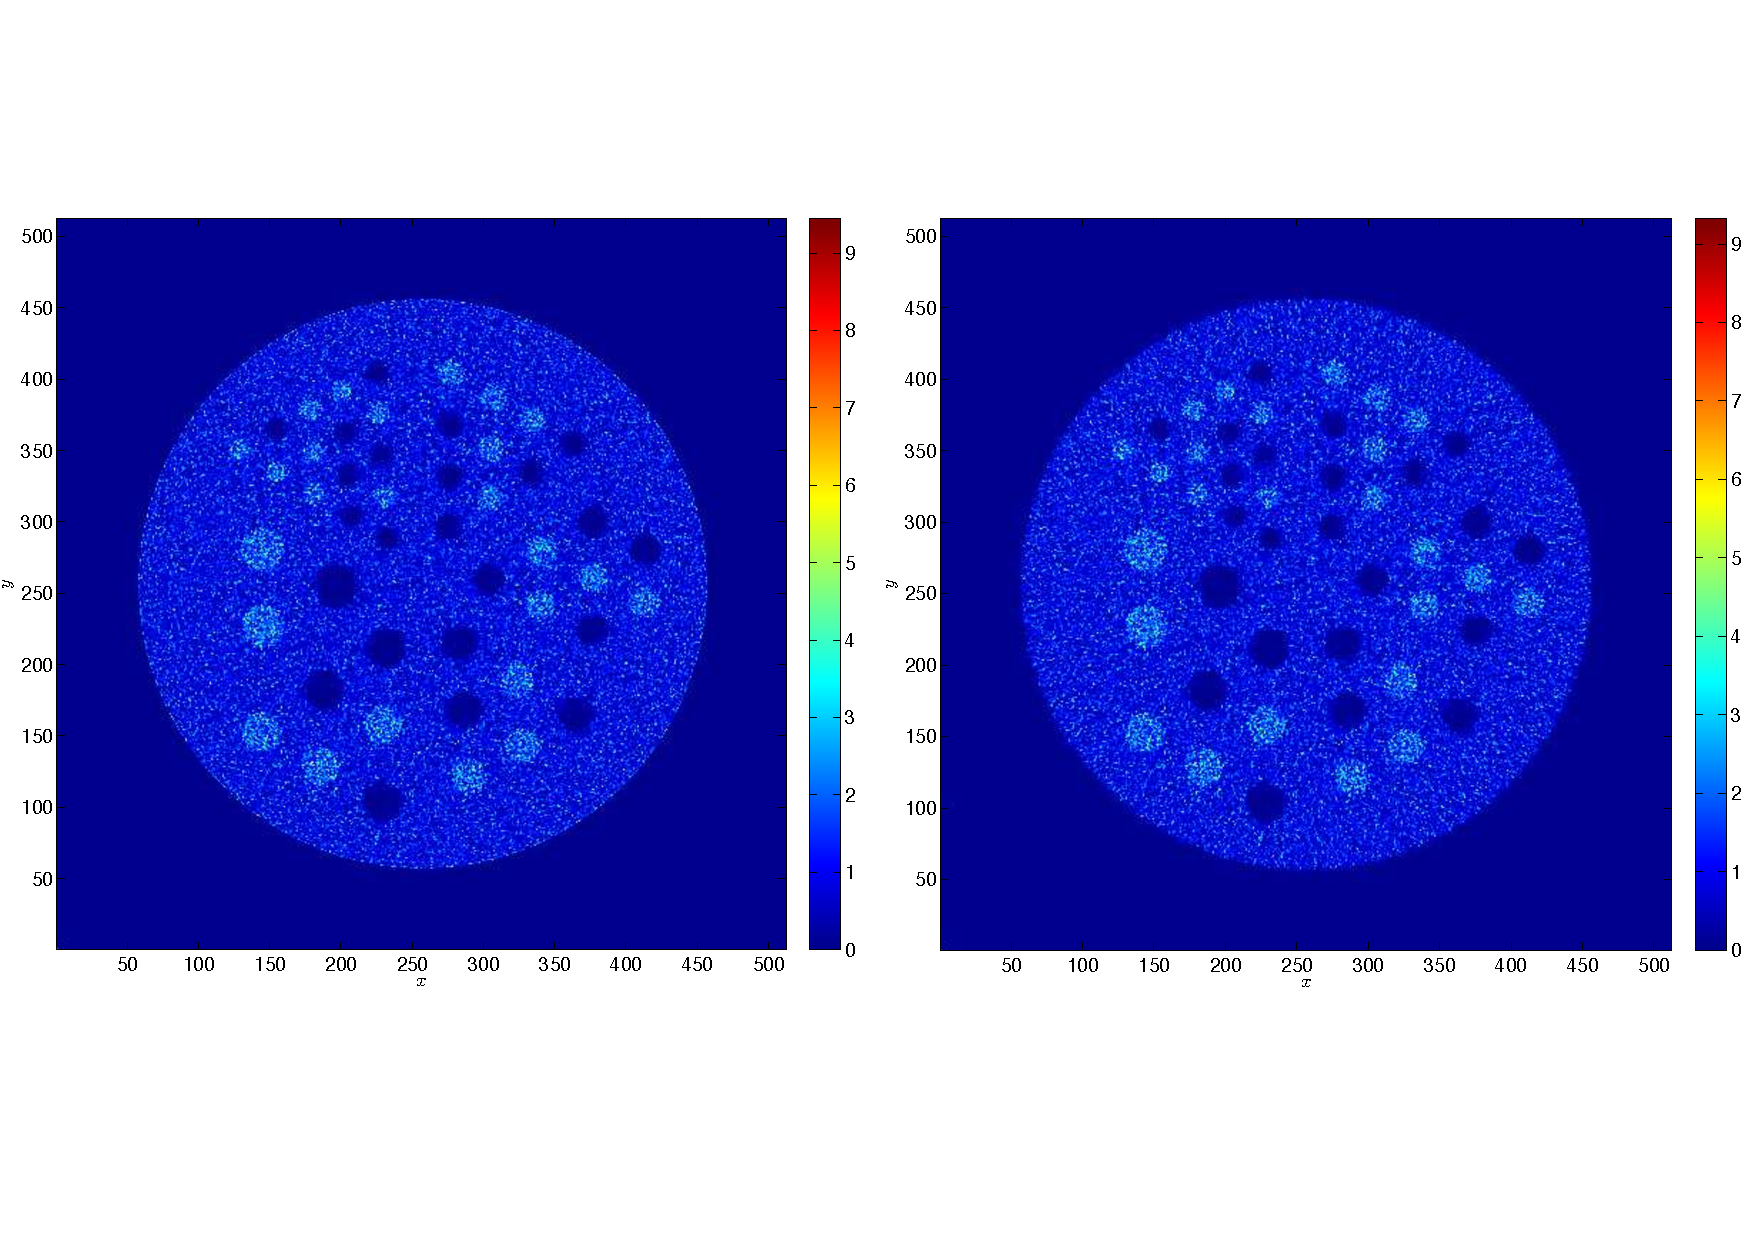
\includegraphics[width=1.01\linewidth]{figures/Appendix7}}
	\caption{Large version of figure \ref{fig:singleReconstruction}\\
	The reconstruction of a single image with MLEM (left) and ISRA (right). As expected, the reconstructed images are less sharp than the expected images in figure \ref{fig:ResultsExpBiasVar200}.}
	\label{fig:a7}
\end{figure}
\bigbreak
\clearpage
\newpage




\begin{figure}
\begin{minipage}[b]{.85\linewidth}
	\centering
	\centerline{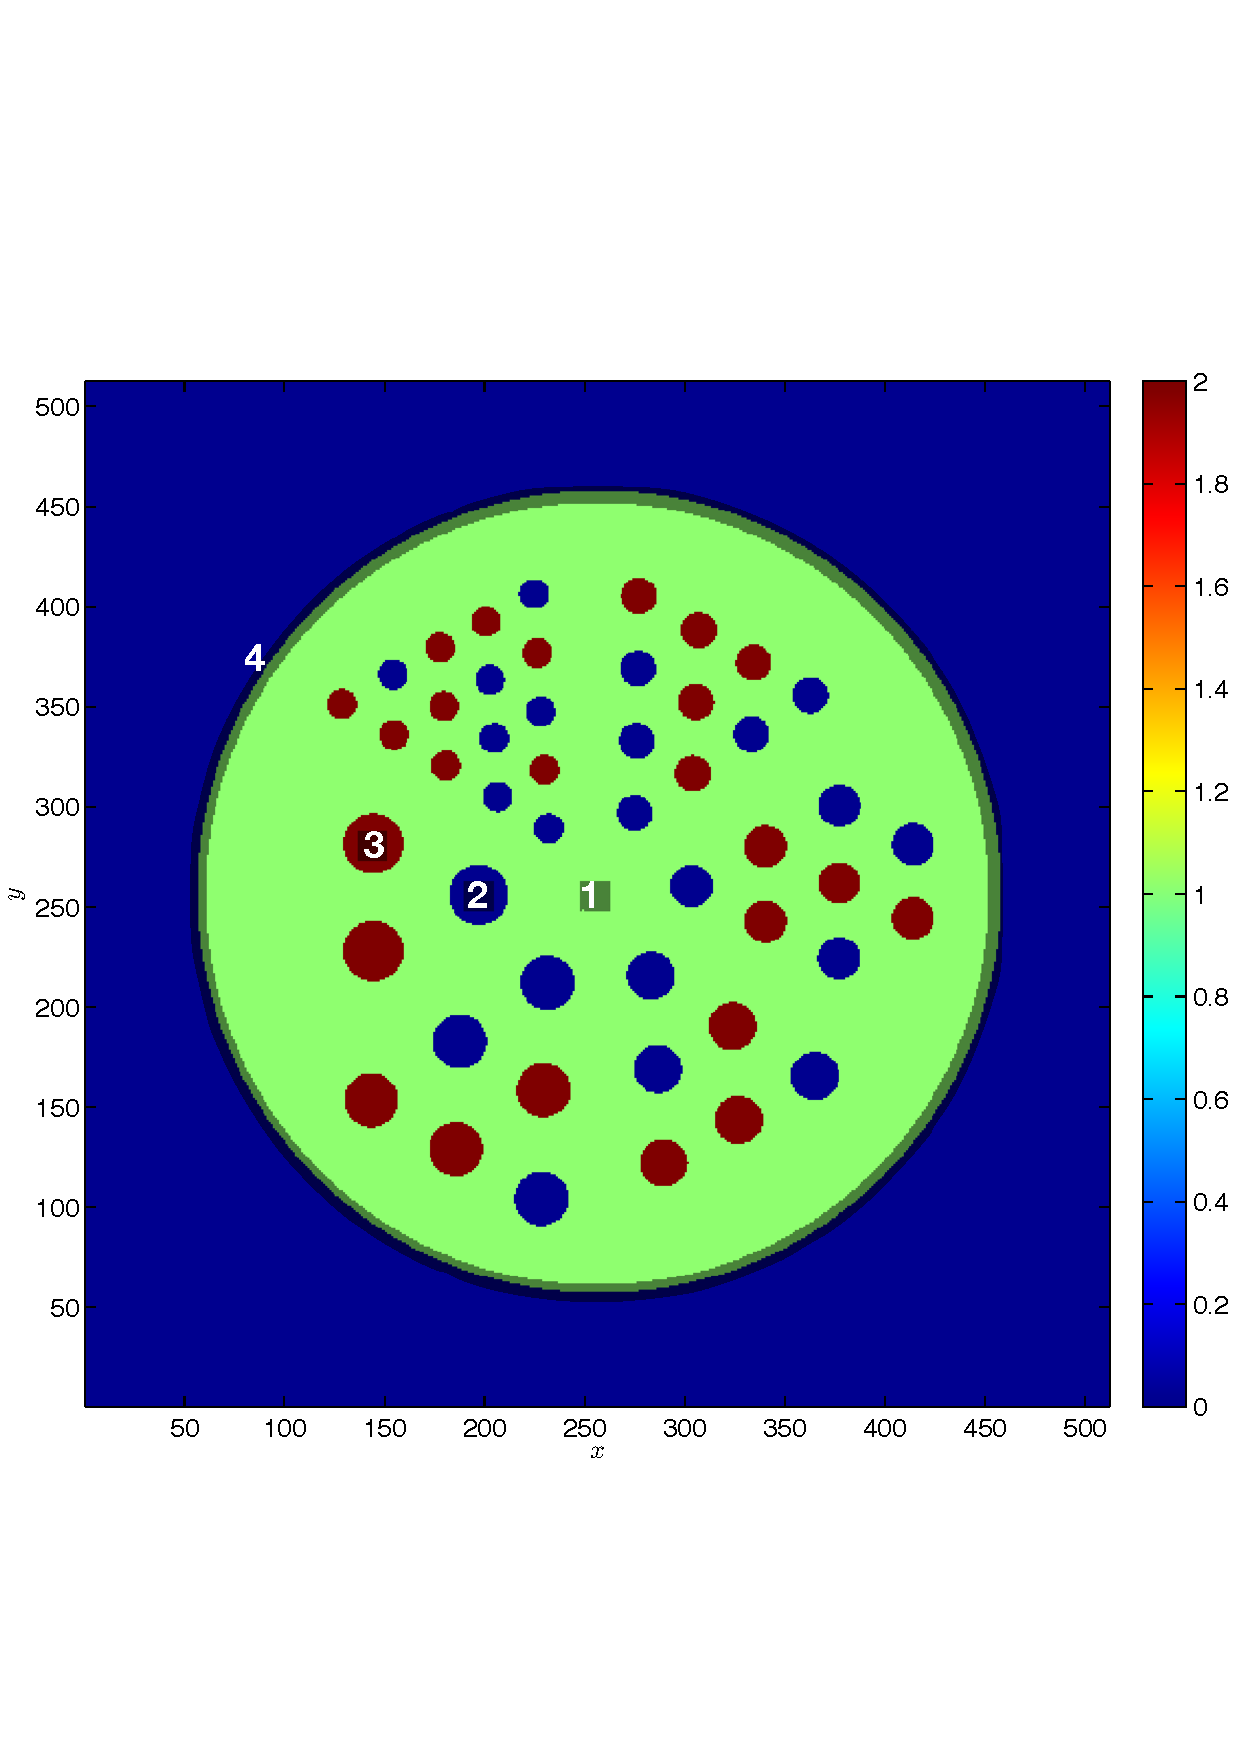
\includegraphics[width=.9\linewidth]{figures/DefRoi}}
	\caption{Large version of figure \ref{fig:roi}\\
	Some specific regions of interest to be examined.}
	\label{fig:a8}
	\end{minipage}
\end{figure}
\bigbreak
\clearpage
\newpage




\begin{figure}[h]
	\centerline{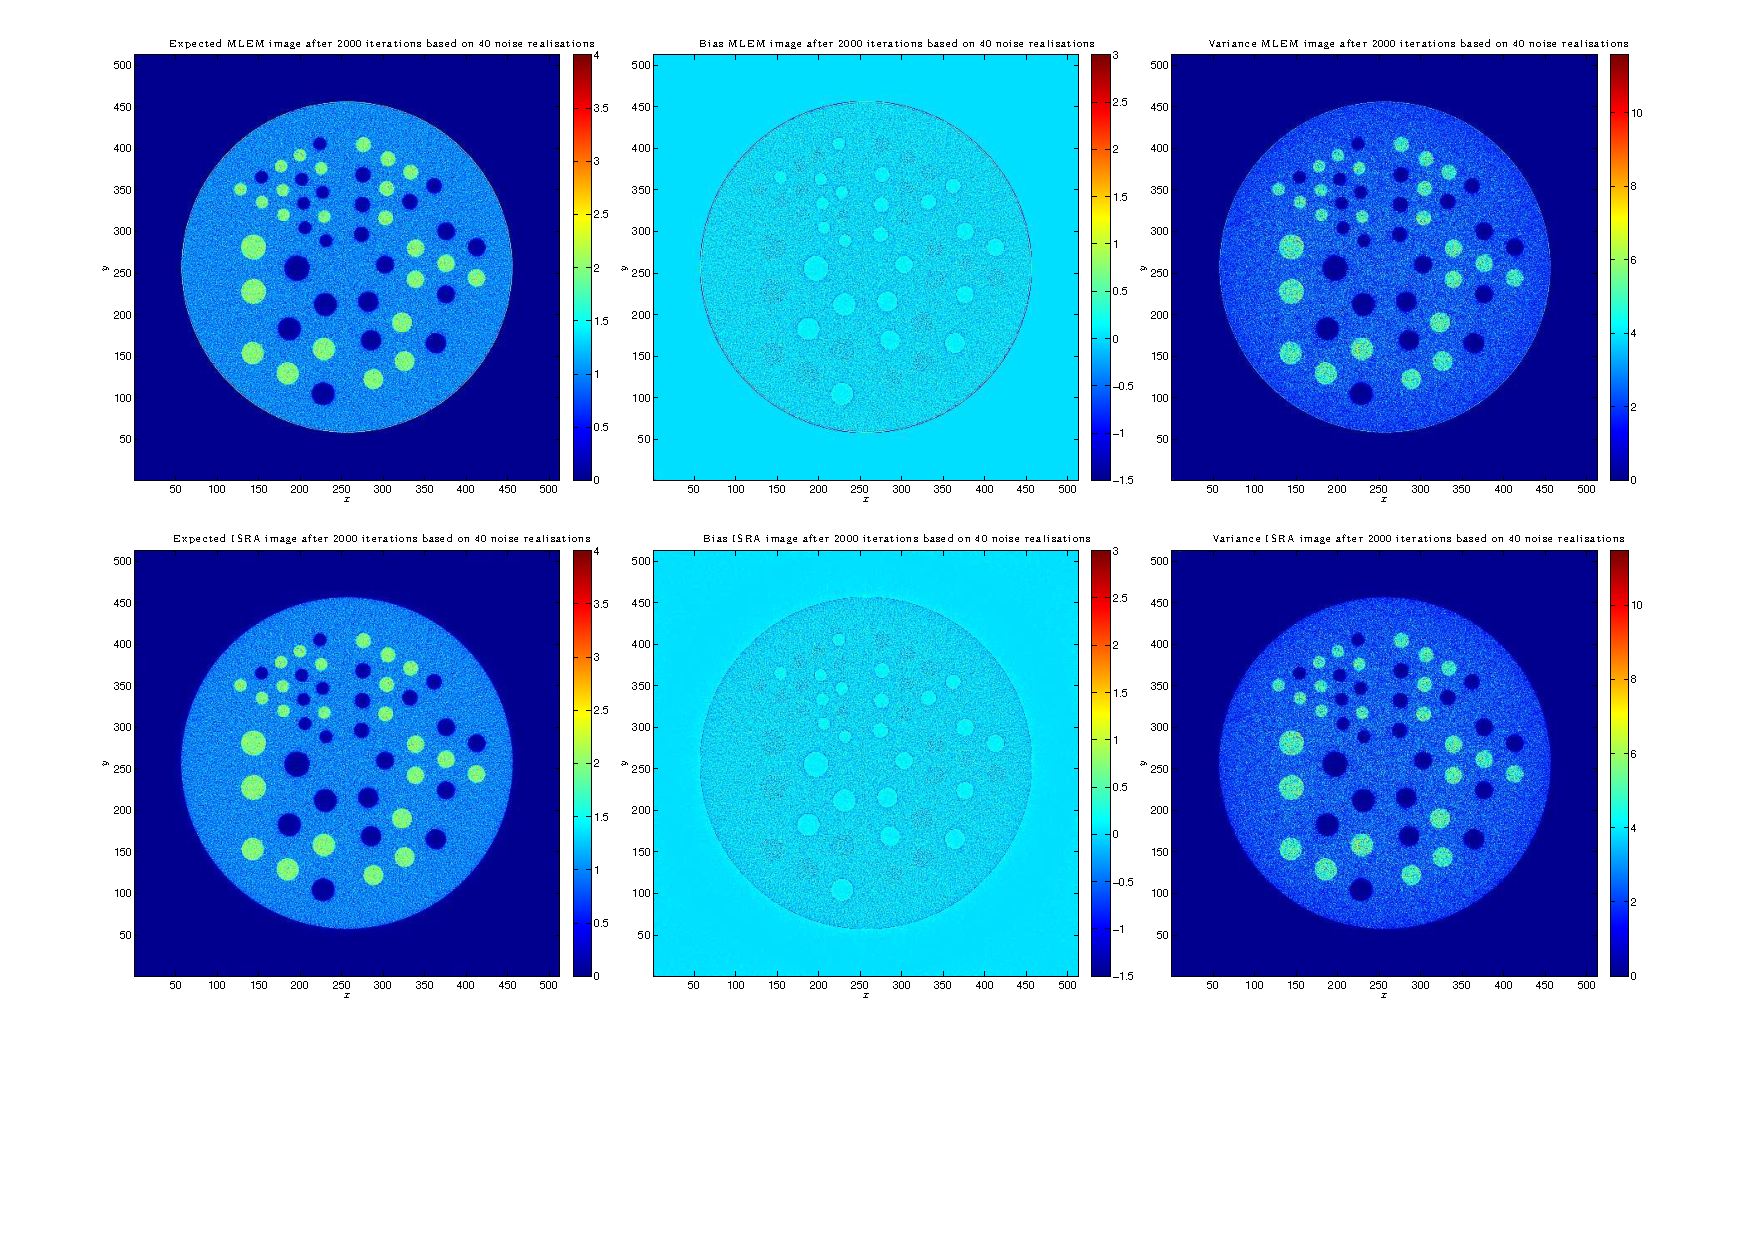
\includegraphics[width=1.08\linewidth]{figures/Appendix9}}
	\caption{Large version of figure \ref{fig:ResultsExpBiasVar2000}\\
	Results obtained after reconstruction with MLEM (top) and ISRA (bottom) with 2000 iterations, based on 40 different noise realisations.}
	\label{fig:a9}
\end{figure}
\bigbreak
\clearpage
\newpage


\end{landscape}

%----------------------------------------------------------------------------
%Bibliografie
%----------------------------------------------------------------------------
\clearpage
\addtocontents{toc}{\vspace{\normalbaselineskip}}
\addcontentsline{toc}{section}{\textbf{References}}
\renewcommand\bibname{References}
\begin{thebibliography}{99}

\bibitem{stat1} A. Abebe, J. Daniels, J.W. McKean, \emph{Statistics and data analysis}, (2000), Western Michingan University.
\\ \url{http://www.stat.wmich.edu/s160/hcopy/book.pdf}

	
\bibitem{stat2} J. D'Hondt, \emph{Statistiche Verwerking van Experimentele Gegevens}, (2012), Vrije Universiteit Brussel.

	
\bibitem{stat3} \emph{Computationele Fysica}, (2015), Vrije Universiteit Brussel.


\bibitem{Watkins} J. Watkins, \emph{Introduction to the science of statistics}, University of Arizona, Topic 14: Unbiassed Estimation
	\\ \url{http://math.arizona.edu/~jwatkins/N_unbiased.pdf}
	
	
\bibitem{cramerRaoMultiDim} \emph{Introduction to the Cramer-Rao bound}, 2017


\bibitem{petscanners} A.M.J. Paans, \emph{Positron emission tomography}, University Medical Center Groningen
\\ \url{https://cds.cern.ch/record/1005065/files/p363.pdf}

	
\bibitem{leastsquare} G. L. Zeng, \emph{Medical image reconstruction: a conceptual tutorial}, Higher education press, 2009.
	
	
\bibitem{proof of ml equal ls} Wikipedia, \emph{Proofs involving ordinary least squares}, last modified on 23 February 2017.
	\\ \url{https://en.wikipedia.org/wiki/Proofs_involving_ordinary_least_squares#Maximum_likelihood_approach}
	
\bibitem{dempster} A.P. Dempster, N.M. Laird, D.B. Rubin, \emph{Maximum Likelihood from Incomplete Data via the EM Algorithm}, (1977), Journal of the Royal Statistical Society. Series B (Methodological), Vol. 39, No. 1 (1977), pp. 1-38
\\ \url{http://www.jstor.org/stable/2984875}
	
	
\bibitem{1982 shepp} Shepp L.A., Vardi Y., \emph{Maximum likelihood estimation for emission tomography }, (1982), IEEE Trans Med Imaging 1: 113 - 121
\\ \url{http://ieeexplore.ieee.org/document/4307558/}
	
	
\bibitem{daube-wither}Daube-Witherspoon M.E., Muehllehner G., \emph{An Iterative Image Space Reconstruction Algorithm Suitable for Volume ECT}, (1986), IEEE Trans Med Imaging vol. mi-5, no. 2: 61 - 66

	
\bibitem{de pierro} De Pierro A.R., \emph{On the Relation Between the ISRA and the EM Algorithm for Positron Emission Tomography}, (1993), IEEE Trans Med Imaging vol. 12, no. 2: pp. 328 - 333 


\bibitem{de pierro 2} De Pierro A.R., \emph{On the convergence of the iterative image space reconstruction algorithm for volume ECT}, (1987), IEEE Trans. Med. Imaging, vol. MI-6, pp. 174-175
 
 
 \bibitem{eggermont} Eggermont P.P.B., \emph{Multiplicative iterative algorithms for convex programming}, (1990), Linear Algebra Appl., vol. 130, pp. 25-42
 
 
 \bibitem{titterington}Titterington D.M., \emph{On the iterative image space reconstruction algorithm for ECT}, (1987), IEEE Trans. Med. Imaging, vol. MI-6, pp. 52-56
 
 
 \bibitem{OSEM} Hudson H. M., Larkin R. S., \emph{Accelerated Image Reconstruction Using Ordered Subsets of Projection Data}, (1994), IEEE Trans. Med. Imaging, vol. 13, no. 4: pp. 601-609
 
 
 \bibitem{china} Fan Xin et al., \emph{PET image reconstruction with system matrix containing point spread function derived from single photon incidence response}, Chinese Academy of Sciences, Beijing Engineering Research Center of Radiographic Techniques and Equipment, University of Chinese Academy of Sciences
\\ \url{https://arxiv.org/pdf/1405.0659.pdf} 
 
 
\bibitem{system matrix errors} L. Fin, P. Bailly, J. Daouk, M.-E. Meyer, \emph{A practical way to improve contrast-to-noise ratio and quantitation for statistical-based iterative reconstruction in whole-body PET imaging}, (2009), Medical Physics 36 (7), 3072 - 3079
\\ \url{https://www.researchgate.net/publication/26734700_A_practical_way_to_improve_contrast-to-noise_ratio_and_quantitation_for_statistical-based_iterative_reconstruction_in_whole-body_PET_imaging}


\bibitem{MLEM and OSEM Deviate} C. Cloquet et al., \emph{MLEM and OSEM Deviate From the Cramer-Rao
Bound at Low Counts}, IEEE transactions on nuclear science, vol. 60, no. 1, February 2013.


\bibitem{Jaszczak} International Atomic Energy Agency, \emph{IAEA human health series, No. 6: Quality Assurance for SPECT Systems}, Vienna : International Atomic Energy Agency, 2009, ISBN:978-92-0-103709-1
	\\ \url{http://www-pub.iaea.org/MTCD/Publications/PDF/Pub1394_web.pdf}
	
	
%\bibitem{radioactivedecay} S.L. Campbell, J.M.G. Duarte, \emph{Poisson Statistics of Radioactive Decay}, (2008), MIT Department of Physics
%\\ \url{http://jacob9.dk/Fysik/Fysikkens\%20Felter/Kernefysik/Diverse/Poisson\%20og\%20Radioaktivitet/radioaktivity\%20poisson\%20paper\%20041012.pdf}
%	
%	
%	\bibitem{Zygouras} N. Zygouras, \emph{Statistics for finance}, 2010, University of Warwick, Lecture 3: Estimation and likelihood
%	\\ \url{https://www2.warwick.ac.uk/fac/sci/statistics/staff/academic-research/zygouras/teaching/lecture3.pdf}
%
%
%	\bibitem{Greene} W.H. Greene, \emph{Econometric analysis}, Pearson, 2010
%	\\ \url{http://people.stern.nyu.edu/wgreene/MathStat/GreeneChapter4.pdf}
 \end{thebibliography} 
\end{document}









































